\documentclass{Class/project_report}
\setTHSarabunFont
\geometry{a4paper,top=1.5in,bottom=1in,left=1.5in,right=1in}
\pagestyle{plain} % ตั้งค่า pagestyle เริ่มต้น
\newcolumntype{L}{>{\RaggedRight\arraybackslash}X} 
\usepackage[smartEllipses]{markdown}
\begin{document}

    % Setup for Figures (centered label and text)
    \captionsetup[figure]{
      font={normalsize},
      labelfont={bold16pt},
      labelsep=quad,
      justification=centering,
      singlelinecheck=false,
      name={ภาพที่} % Add this line
    }
    % Setup for Tables (raggedright label and text)
    \captionsetup[table]{
      font={normalsize},
      labelfont={bold16pt},
      labelsep=quad,
      justification=raggedright,
      singlelinecheck=false,
      skip=8pt,
      indention=0.9in,
      name={ตารางที่} % Add this line
    }
    %*************************************
% ปกนอก
%*************************************
\newpage
\thispagestyle{empty}
\begin{center}

\vspace*{-0.8in}


\includegraphics[width=5.08cm]{Image/Logo_KMUTNB_Thai.png}
\vspace{2mm}

{\bf
    แพลตฟอร์มคลัสเตอร์เพื่อสนับสนุนการเรียนการสอน \\
    และงานวิชาการภาควิชาเทคโนโลยีสารสนเทศ %ชื่อโปรเจ็คภาษาไทย
}

\vspace{0.3in}

% กรณีทำโปรเจ็คคนเดียว 
\vspace{60mm}
{\bf
   นายฐิติพงษ์ ตะเพียนทอง %ชื่อผู้จัดทำ
}
\vspace{64mm}   

% \vspace{0.4in}


% กรณีมีเพื่อนร่วมทำโปรเจ็ค
% \vspace{56mm}
% {\bf
%     % นางสาวสุพาภรณ์ ซิ้มเจริญ    %ชื่อผู้จัดทำ1
%     \\
%     % นางสาวสิวาลัย จินเจือ       %ชื่อผู้จัดทำ2
% }
% \vspace{60mm}  




{\bf 
    %----------------------------------------------------
    % กรณีเป็นนักศึกษาหลักสูตร IT
    % ปริญญานิพนธ์นี้เป็นส่วนหนึ่งของการศึกษาตามหลักสูตรวิทยาศาสตรบัณฑิต\\
    % สาขาวิชาเทคโนโลยีสารสนเทศ ภาควิชาเทคโนโลยีสารสนเทศ\\
    
    % กรณีเป็นนักศึกษาหลักสูตร ITI
    %ปริญญานิพนธ์นี้เป็นส่วนหนึ่งของการศึกษาตามหลักสูตรอุตสาหกรรมศาสตรบัณฑิต\\
    %สาขาวิชาเทคโนโลยีสารสนเทศ (ต่อเนื่อง) ภาควิชาเทคโนโลยีสารสนเทศ\\
    
    % กรณีเป็นนักศึกษาหลักสูตร INE และ INET
    ปริญญานิพนธ์นี้เป็นส่วนหนึ่งของการศึกษาตามหลักสูตรวิศวกรรมศาสตรบัณฑิต\\
    สาขาวิชาวิศวกรรมสารสนเทศและเครือข่าย ภาควิชาเทคโนโลยีสารสนเทศ\\
    
    %----------------------------------------------------
    คณะเทคโนโลยีและการจัดการอุตสาหกรรม มหาวิทยาลัยเทคโนโลยีพระจอมเกล้าพระนครเหนือ    \\
    ปีการศึกษา 2568\\
    ลิขสิทธิ์ของมหาวิทยาลัยเทคโนโลยีพระจอมเกล้าพระนครเหนือ
}

\end{center}

%*************************************
% ปกในภาษาไทย
%*************************************
\newpage
\thispagestyle{empty}
\begin{center}

\vspace*{-0.5in}

แพลตฟอร์มคลัสเตอร์เพื่อสนับสนุนการเรียนการสอนและงานวิชาการภาควิชาเทคโนโลยีสารสนเทศ     %ชื่อโปรเจ็คภาษาไทย

\vspace{0.1in}
%----------------------------------------------------

% กรณีทำโปรเจ็คคนเดียว 
\vspace{90mm}
นายฐิติพงษ์ ตะเพียนทอง %ชื่อผู้จัดทำ
\vspace{94mm}   

\vspace{0.1in}

% กรณีมีเพื่อนร่วมทำโปรเจ็ค
%\vspace{86mm}
%นางสาวสุพาภรณ์ ซิ้มเจริญ    %ชื่อผู้จัดทำ1
%\\
%นางสาวสิวาลัย จินเจือ       %ชื่อผู้จัดทำ2
%\vspace{90mm}  

%----------------------------------------------------
% กรณีเป็นนักศึกษาหลักสูตร IT
% ปริญญานิพนธ์นี้เป็นส่วนหนึ่งของการศึกษาตามหลักสูตรวิทยาศาสตรบัณฑิต\\
% สาขาวิชาเทคโนโลยีสารสนเทศ ภาควิชาเทคโนโลยีสารสนเทศ\\

% กรณีเป็นนักศึกษาหลักสูตร ITI
%ปริญญานิพนธ์นี้เป็นส่วนหนึ่งของการศึกษาตามหลักสูตรอุตสาหกรรมศาสตรบัณฑิต\\
%สาขาวิชาเทคโนโลยีสารสนเทศ (ต่อเนื่อง) ภาควิชาเทคโนโลยีสารสนเทศ\\

% กรณีเป็นนักศึกษาหลักสูตร INE และ INET
ปริญญานิพนธ์นี้เป็นส่วนหนึ่งของการศึกษาตามหลักสูตรวิศวกรรมศาสตรบัณฑิต\\
สาขาวิชาวิศวกรรมสารสนเทศและเครือข่าย ภาควิชาเทคโนโลยีสารสนเทศ\\

%----------------------------------------------------
คณะเทคโนโลยีและการจัดการอุตสาหกรรม มหาวิทยาลัยเทคโนโลยีพระจอมเกล้าพระนครเหนือ\\
ปีการศึกษา 2568\\
ลิขสิทธิ์ของมหาวิทยาลัยเทคโนโลยีพระจอมเกล้าพระนครเหนือ

\end{center}


%*************************************
% ปกในภาษาอังกฤษ
%*************************************
\newpage
\thispagestyle{empty}
\begin{center}

\vspace*{-0.5in}

CLUSTER-BASED PLATFORM FOR SUPPORTING TEACHING AND ACADEMIC ACTIVITIES \\
IN THE DEPARTMENT OF INFORMATION TECHNOLOGY %ชื่อโปรเจ็คภาษาอังกฤษ

\vspace{0.2in}

% กรณีทำโปรเจ็คคนเดียว 
\vspace{80mm}
MR.THITIPONG TAPIANTHONG      %ชื่อผู้จัดทำ
\vspace{76.5mm}   


% กรณีมีเพื่อนร่วมทำโปรเจ็ค
%\vspace{76mm}
%MS.SUPAPORN SIMCHAROEN       %ชื่อผู้จัดทำ1
%\\
%MS.SIWALAI CHINCHUA          %ชื่อผู้จัดทำ2
%\vspace{80mm}  

\vspace{0.2in}

ROJECT REPORT SUBMITTED IN PARTIAL FULFILLMENT OF THE REQUIREMENTS \\
%----------------------------------------------------

% กรณีเป็นนักศึกษาหลักสูตร IT
% FOR THE BACHELOR’S DEGREE OF SCIENCE\\
% PROGRAM IN INFORMATION TECHNOLOGY\\

% กรณีเป็นนักศึกษาหลักสูตร ITI
%FOR THE BACHELOR’S DEGREE OF INDUSTRIAL TECHNOLOGY\\ 
%PROGRAM IN INFORMATION TECHNOLOGY (CONTINUING PROGRAM)\\

% กรณีเป็นนักศึกษาหลักสูตร INE และ INET
FOR THE BACHELOR’S DEGREE OF ENGINEERING\\
PROGRAM IN INFORMATION AND NETWORK ENGINEERING\\

%----------------------------------------------------
DEPARTMENT OF INFORMATION TECHNOLOGY\\
FACULTY OF INDUSTRIAL TECHNOLOGY AND MANAGEMENT\\
KING MONGKUT’S UNIVERSITY OF TECHNOLOGY NORTH BANGKOK\\
ACADEMIC YEAR 2025\\
COPYRIGHT OF KING MONGKUT’S UNIVERSITY OF TECHNOLOGY NORTH BANGKOK

\end{center}

    
    %**************************************************************************************
% ใบรับรองโครงงาน กรณี ไม่มี ที่ปรึกษาร่วม
%**************************************************************************************
\newpage
\thispagestyle{empty}
\setstretch{1.25}
\setlength{\parindent}{0pt}

\vspace*{-0.5in}

\begin{tcolorbox}[colframe=black, colback=white, width=\textwidth, boxrule=0.8pt, arc=1mm, auto outer arc, left=10pt, right=10pt, top=10pt, bottom=10pt, enhanced jigsaw]

\begin{center}
\vspace{3mm}

\includegraphics[width=3.18cm]{Image/Logo_KMUTNB_Thai.png}

{\bf {\fontTwentyFour
    ใบรับรองปริญญานิพนธ์
    \\
}{\fontEighteen
    คณะเทคโนโลยีและการจัดการอุตสาหกรรม
    \\
    มหาวิทยาลัยเทคโนโลยีพระจอมเกล้าพระนครเหนือ
}}
\end{center}
\vspace{1em}
\fontSixTeen{
\begin{tabbing}
    เรื่อง  \= แพลตฟอร์มคลัสเตอร์เพื่อสนับสนุนการเรียนการสอนและงานวิชาการ
    \\   \> ภาควิชาเทคโนโลยีสารสนเทศ       %ชื่อโปรเจ็คภาษาไทย
    \\
    โดย  \> นายฐิติพงษ์ ตะเพียนทอง     %ชื่อผู้จัดทำ1 
    %\\     %เว้นบรรทัด เมื่อมีเพื่อนร่วมโปรเจ็ค
        %\> นางสาวสิวาลัย จินเจือ       %ชื่อผู้จัดทำ2
    \\
    \\
         \> ได้รับอนุมัติให้นับเป็นส่วนหนึ่งของการศึกษาตาม 
    \\
         % \> หลักสูตรวิทยาศาสตรบัณฑิต  สาขาวิชาเทคโนโลยีสารสนเทศ % กรณีเป็นนักศึกษาหลักสูตร IT
         %\> หลักสูตรอุตสาหกรรมศาสตรบัณฑิต  สาขาวิชาเทคโนโลยีสารสนเทศ (ต่อเนื่อง) % กรณีเป็นนักศึกษาหลักสูตร ITI
         \> หลักสูตรวิศวกรรมศาสตรบัณฑิต  สาขาวิชาวิศวกรรมสารสนเทศและเครือข่าย % กรณีเป็นนักศึกษาหลักสูตร INE และ INET
      
\end{tabbing}

\vspace{1.5em}

\begin{flushright}
\makebox[8cm][l]{\rule{7cm}{0.4pt} คณบดี} \\
\makebox[8cm][l]{(ผู้ช่วยศาสตราจารย์ ดร.กฤษฎากร  บุดดาจันทร์)}
\end{flushright}


\vspace{14mm}  %กรณีทำโปรเจ็คคนเดียว
%\vspace{8mm}  %กรณีมีเพื่อนร่วมโปรเจ็ค


\vspace{0.2in}

คณะกรรมการสอบปริญญานิพนธ์

\vspace{1.5em}
\begin{flushleft}
\makebox[7cm][l]{\rule{7cm}{0.4pt} ประธานกรรมการ} \\
\makebox[7cm][c]{(ผู้ช่วยศาสตราจารย์ ดร.ศรายุทธ ธเนศสกุลวัฒนา)}       %ระบุชื่อประธานกรรมการ
\end{flushleft}

\vspace{1.5em}
\begin{flushleft}
\makebox[7cm][l]{\rule{7cm}{0.4pt} กรรมการ} \\
\makebox[7cm][c]{(อาจารย์ ดร.วัชรชัย คงศิริวัฒนา)}            %ระบุชื่อกรรมการ
\end{flushleft}

\vspace{1.5em}
\begin{flushleft}
\makebox[7cm][l]{\rule{7cm}{0.4pt} กรรมการ} \\
\makebox[7cm][c]{(ผู้ช่วยศาสตราจารย์ ดร.ขนิษฐา นามี)}       %ระบุชื่ออาจารย์ที่ปรึกษาโปรเจ็ค
\end{flushleft}

} %end fontSixTeen
\end{tcolorbox}
 %กรณี ไม่มี ที่ปรึกษาร่วม
    %\input{Project_001_Certificate2} %กรณี มี ที่ปรึกษาร่วม

    
    \newpage
    \thaiPageStyle
    \setcounter{page}{2}
    \fontSixTeen
    \justifying
    %**************************************************************************************
% บทคัดย่อภาษาไทย
%**************************************************************************************
\phantomsection
\addcontentsline{toc}{chapter}{บทคัดย่อภาษาไทย}
\vspace*{-0.5in}

\begin{tabularx}{\textwidth}{lX}
ชื่อ                           & : นายฐิติพงษ์ ตะเพียนทอง         %ชื่อผู้จัดทำ1 
%\\     %เว้นบรรทัด เมื่อมีเพื่อนร่วมโปรเจ็ค
%                             & : นางสาวสิวาลัย จินเจือ            %ชื่อผู้จัดทำ2 
\\
ชื่อปริญญานิพนธ์                  & : \hangindent=0.5em          % มีไว้สำหรับตอนชื่อโปรเจ็คเกิน 1 บรรทัด
                                แพลตฟอร์มคลัสเตอร์เพื่อสนับสนุนการเรียนการสอนและงานวิชาการภาควิชาเทคโนโลยีสารสนเทศ  %ระบุชื่อโปรเจ็คภาษาไทย
\\
% สาขาวิชา                       & : เทคโนโลยีสารสนเทศ % กรณีเป็นนักศึกษาหลักสูตร IT
%สาขาวิชา                       & : เทคโนโลยีสารสนเทศ (ต่อเนื่อง) % กรณีเป็นนักศึกษาหลักสูตร ITI
สาขาวิชา                       & : วิศวกรรมสารสนเทศและเครือข่าย % กรณีเป็นนักศึกษาหลักสูตร INE และ INET
\\
                             & : มหาวิทยาลัยเทคโนโลยีพระจอมเกล้าพระนครเหนือ
\\
อาจารย์ที่ปรึกษาปริญญานิพนธ์        & : ผู้ช่วยศาสตราจารย์ ดร.ขนิษฐา นามี    %ระบุชื่ออาจารย์ที่ปรึกษา
%\\      %เว้นบรรทัด เมื่อมีที่ปรึกษาร่วม
%ที่ปรึกษาร่วม                    & : ผู้ช่วยศาสตาจารย์ ดร.นิติการ นาคเจือทอง    %ระบุชื่อที่ปรึกษาร่วม (ถ้ามี)
\\
ปีการศึกษา                     & : 2568     %ระบุปีการศึกษา
\end{tabularx}

\vspace{5mm}
\phantomsection
\begin{center}\textbf{บทคัดย่อ}\end{center}
\hspace*{1.5em} %ย่อหน้า
ปริญญานิพนธ์ "แพลตฟอร์มคลัสเตอร์เพื่อสนับสนุนการเรียนการสอนและงานวิชาการภาควิชาเทคโนโลยีสารสนเทศ" ฉบับนี้ มีวัตถุประสงค์เพื่อพัฒนาแพลตฟอร์มคลัสเตอร์เสมือนที่สามารถสร้างและจัดการเครื่องเสมือนลีนุกซ์ได้อย่างรวดเร็วและมีประสิทธิภาพ เพื่อสนับสนุนการเรียนการสอนและการทำโครงงานในภาควิชาเทคโนโลยีสารสนเทศ และพัฒนาเว็บแอปพลิเคชันแบบ Role-Based Access Control (RBAC) ที่รองรับการใช้งานของทั้งนักศึกษาและอาจารย์ โดยคำนึงถึงความง่ายในการใช้งาน เสถียรภาพของระบบ และความปลอดภัยในการเข้าถึง ระบบประกอบด้วยสามส่วนหลัก ได้แก่ ส่วนติดต่อผู้ใช้งาน บริการ API สำหรับจัดการการยืนยันตัวตน การจัดการผู้ใช้ และเชื่อมต่อระหว่างส่วนติดต่อผู้ใช้และบริการจัดการเครื่องเสมือน และบริการจัดการเครื่องเสมือนที่เชื่อมต่อกับระบบ Hypervisor เพื่อสร้าง กำหนดค่า และจัดการเครื่องเสมือน ระบบสามารถลดความซับซ้อนในการตั้งค่าสภาพแวดล้อมสำหรับการใช้งานระบบลีนุกซ์ เพิ่มประสิทธิภาพการใช้ทรัพยากรเซิร์ฟเวอร์ และสนับสนุนการเรียนการสอนที่เกี่ยวข้องกับระบบเซิร์ฟเวอร์ การพัฒนาแอปพลิเคชัน และการจัดการโครงสร้างพื้นฐานด้านไอทีได้อย่างมีประสิทธิภาพ

\begin{flushright}
(ปริญญานิพนธ์มีจำนวนทั้งสิ้น \pageref{LastPage} หน้า)

\vfill
\rule{10 cm}{0.4pt} อาจารย์ที่ปรึกษาปริญญานิพนธ์ 
%\\ \vspace{3mm}                        %เว้นกรณีมีที่ปรึกษาร่วม
%\rule{12.6 cm}{0.4pt} ที่ปรึกษาร่วม         % กรณีมีที่ปรึกษาร่วม

\end{flushright}





%**************************************************************************************
% บทคัดย่อภาษาอังกฤษ
%**************************************************************************************
\newpage
\phantomsection
\addcontentsline{toc}{chapter}{บทคัดย่อภาษาอังกฤษ}
\vspace*{-0.5in}

\begin{tabularx}{\textwidth}{lX}
Name                    & : Mr.Thitipong Tapianthong  %ชื่อผู้จัดทำ1
%\\      %เว้นบรรทัดเมื่อมีเพื่อนร่วมโปรเจ็ค
%                       & : Ms.Siwalai Chinchua      %ชื่อผู้จัดทำ2
\\
Project Title           & : \hangindent=0.5em % มีไว้สำหรับตอนชื่อโปรเจ็คเกิน 1 บรรทัด
                            Cluster-Based Platform for Supporting Teaching and
                            Academic Activities in the Department of Information Technology  %ระบุชื่อโปรเจ็คภาษาอังกฤษ
\\
% Major Field             & : Information Technology % กรณีเป็นนักศึกษาหลักสูตร IT
%Major Field             & : Information Technology (Continuing Program) % กรณีเป็นนักศึกษาหลักสูตร ITI
Major Field             & : Information and Network Engineering % กรณีเป็นนักศึกษาหลักสูตร INE และ INET
\\
                        & : King Mongkut’s University of Technology North Bangkok
\\
Project Advisor         & : Asst. Prof. Dr.Khanista Namee   %ระบุชื่ออาจารย์ที่ปรึกษา
%\\      %เว้นบรรทัด เมื่อมีที่ปรึกษาร่วม
%Co-Advisor              & : Asst. Prof. Dr.Nitigan Nakjuatong   %ระบุชื่อที่ปรึกษาร่วม (ถ้ามี)
\\
Academic Year           & : 2025    %ระบุปีการศึกษา
\end{tabularx}

\vspace{5mm}
\begin{center}\textbf{Abstract}\end{center}

\hspace*{1.5em} %ย่อหน้า
This project, "Cluster-Based Platform for Supporting Teaching and Academic Activities in the Department of Information Technology," aims to develop a virtual cluster platform capable of rapidly and efficiently creating and managing Linux virtual machines to support teaching and project work in the Department of Information Technology. The project also focuses on developing a Role-Based Access Control (RBAC) web application that supports both students and faculty, emphasizing ease of use, system stability, and access security. The system consists of three main components: a user interface, an API service for handling authentication and user management and communication between the frontend and VM operations service, and a VM management service that interfaces with the Hypervisor system to create, configure, and manage virtual machines. The system reduces the complexity of setting up Linux environments, improves server resource utilization efficiency, and effectively supports teaching related to server systems, application development, and IT infrastructure management.

\begin{flushright}
(Total \pageref{LastPage} pages)

\vfill

\rule{12 cm}{0.4pt} Project Advisor
%\\ \vspace{3mm}                          %เว้นกรณีมีที่ปรึกษาร่วม
%\rule{12.7 cm}{0.4pt} Co-Advisor         % กรณีมีที่ปรึกษาร่วม

\end{flushright}


%**************************************************************************************
% กิตติกรรมประกาศ
%**************************************************************************************
\newpage
\phantomsection
\addcontentsline{toc}{chapter}{กิตติกรรมประกาศ}
\vspace*{-0.5in}

\begin{center}\textbf{กิตติกรรมประกาศ}\end{center}

\hspace*{1.5em}  %ย่อหน้า
ปริญญานิพนธ์ "แพลตฟอร์มคลัสเตอร์เพื่อสนับสนุนการเรียนการสอนและงานวิชาการภาควิชาเทคโนโลยีสารสนเทศ" จะไม่สามารถสำเร็จลุล่วงไปได้ด้วยดีหากไม่ได้รับการช่วยเหลือและความอนุเคราะห์จากบุคคลหลายท่าน ทางผู้จัดทำขอขอบพระคุณ ผู้ช่วยศาสตราจารย์ ดร.ขนิษฐา นามี ซึ่งเป็นอาจารย์ที่ปรึกษา ที่ได้กรุณาให้คำปรึกษาแนะนำ และให้แนวทางในการพัฒนาแพลตฟอร์มคลัสเตอร์และการจัดทำปริญญานิพนธ์ รวมทั้งคณาจารย์ภาควิชาเทคโนโลยีสารสนเทศที่ได้ให้ความรู้ด้านเทคโนโลยีและการพัฒนาระบบให้กับผู้จัดทำเพื่อนำมาประยุกต์ในการพัฒนาโครงงานนี้ อีกทั้งขอขอบคุณภาควิชาเทคโนโลยีสารสนเทศที่ให้การสนับสนุนโครงสร้างพื้นฐานและทรัพยากรที่จำเป็นสำหรับการพัฒนาและทดสอบระบบ 
\\
\hspace*{1.5em}  %ย่อหน้า
ท้ายที่สุดนี้ ทางผู้จัดทำขอน้อมรำลึกพระคุณบิดา มารดา ผู้ซึ่งมีพระคุณอย่างสูงสุดที่ให้ความอุปการะผู้จัดทำมาโดยตลอด รวมทั้งผู้มีพระคุณทุกท่าน คณะผู้จัดทำรู้สึกซาบซึ้งเป็นอย่างยิ่ง จึงใคร่ขอขอบพระคุณเป็นอย่างสูงมา ณ โอกาสนี้ด้วย
\\
\begin{flushright}
\makebox[6cm][l]{{ฐิติพงษ์ ตะเพียนทอง}}      %ชื่อผู้จัดทำ1
%\\     %เว้นบรรทัด เมื่อมีเพื่อนร่วมโปรเจ็ค
%\makebox[6cm][l]{สิวาลัย จินเจือ}         %ชื่อผู้จัดทำ2

\end{flushright}
    \newgeometry{a4paper,top=1.5in,bottom=1in,left=1.5in,right=1in,includehead}
    \setTHSarabunFont
    \fontsize{16}{16}\selectfont
    \thaiPageStyle
    \customTOCthai
    \newpage
    \customLOFthai
    \newpage
    \customLOTthai
    \clearpage % ขึ้นหน้าใหม่หลังจากหน้าที่มีการปรับ margin
    \restoregeometry % คืนค่า geometry กลับเป็นค่าเริ่มต้น
    \fancyhf{} % ล้างการตั้งค่า fancyhdr ของหน้าที่ปรับ
    \setTHSarabunFont
    \fontsize{16}{16}\selectfont
    \thaiPageStyle
    
    \newpage
    \setlength{\headheight}{0cm}
    \setcounter{page}{1}
    \arabicPageTopRight % ตั้งค่าต่อไปใช้สไตล์อารบิกมุมขวาบน
    \customTOCarabic
    %*************************************
% บทที่ 1
%*************************************
\chapterTitle{1}{บทนำ}

%*******************************************
% ความเป็นมาและความสำคัญ
%*******************************************
\section{ความเป็นมาและความสำคัญ} 

%ระบุความเป็นมาและความสำคัญของโปรเจ็ค
\hspace*{1.3em} %ย่อหน้า
การเรียนการสอนในภาควิชาเทคโนโลยีสารสนเทศมีความจำเป็นต้องใช้ระบบปฏิบัติการลีนุกซ์ในหลายรายวิชา โดยเฉพาะในรายวิชาที่เกี่ยวข้องกับระบบเซิร์ฟเวอร์ การพัฒนาแอปพลิเคชัน และการจัดการโครงสร้างพื้นฐานด้านเทคโนโลยีสารสนเทศ อย่างไรก็ตาม การเตรียมสภาพแวดล้อมสำหรับการใช้งานระบบลีนุกซ์นั้นมักมีความยุ่งยากและใช้เวลานาน ทั้งในด้านการติดตั้ง การตั้งค่า และการจัดการทรัพยากร ส่งผลให้การเรียนการสอนไม่สามารถดำเนินไปได้อย่างเต็มประสิทธิภาพ

\hspace*{1.3em}
ที่ผ่านมา นักศึกษาและอาจารย์ต้องใช้วิธีการจำลองระบบลีนุกซ์ผ่านเครื่องเสมือน (Virtual Machine), ระบบย่อยของวินโดว์สำหรับลีนุกซ์ (WSL), หรือบริการคลาวด์จากภายนอก ซึ่งแต่ละวิธีมีข้อจำกัด เช่น ความยุ่งยากในการตั้งค่า ความไม่เสถียรของระบบ หรือค่าใช้จ่ายเพิ่มเติมในการใช้งานบริการจากผู้ให้บริการภายนอก โดยเฉพาะในการทำโครงงานที่ต้องใช้เซิร์ฟเวอร์ นักศึกษามักต้องจัดหาเครื่องคอมพิวเตอร์ส่วนตัวหรือเซิร์ฟเวอร์ด้วยตนเอง ซึ่งเป็นภาระทั้งด้านเวลาและงบประมาณ

\hspace*{1.3em}
เพื่อแก้ไขปัญหาดังกล่าวข้างต้น โครงงานนี้จึงมีแนวคิดในการพัฒนาแพลตฟอร์มคลัสเตอร์ภายในภาควิชา โดยใช้เทคโนโลยี Virtualization ร่วมกับระบบ cloud-Init เพื่อสร้างเครื่องจำลองลีนุกซ์ที่สามารถใช้งานได้อย่างรวดเร็วและง่ายดาย พร้อมทั้งมีระบบ Web Application สำหรับการจัดการและเข้าใช้งานเครื่องเสมือน ทั้งในส่วนของนักศึกษาและอาจารย์



%*******************************************
% วัตถุประสงค์ของโครงงาน
%*******************************************
\section{วัตถุประสงค์ของโครงงาน}

%ระบุวัตถุประสงค์ของโปรเจ็ค
\begin{mycustomenum}[label=1.2.\arabic*] %เพิ่มวัตถุประสงค์หลัง \item ถ้ามีหลายข้อ ก็เพิ่มบรรทัด \item ไปได้เรื่อย ๆ
    \item เพื่อออกแบบและพัฒนาแพลตฟอร์มคลัสเตอร์เสมือน (Virtual Cluster Platform) ที่สามารถสร้างและจัดการเครื่องเสมือนลีนุกซ์ได้อย่างรวดเร็วและมีประสิทธิภาพ สำหรับสนับสนุนการเรียนการสอนและการทำโครงงานในภาควิชาเทคโนโลยีสารสนเทศ
    \item เพื่อพัฒนา Web Application แบบ Role-Based Access Control (RBAC) ที่รองรับการใช้งานของทั้งนักศึกษาและอาจารย์ ในการร้องขอ จัดการ และเข้าถึงเครื่องเสมือน โดยคำนึงถึงความง่ายในการใช้งาน เสถียรภาพของระบบ และความปลอดภัยในการเข้าถึงแพลตฟอร์ม
    \newpage
    \item เพื่อเพิ่มประสิทธิภาพการใช้ทรัพยากรเซิร์ฟเวอร์ที่มีอยู่ภายในภาควิชา ผ่านการพัฒนาระบบคลัสเตอร์แบบรวมศูนย์ ที่สามารถติดตาม วิเคราะห์ และบริหารจัดการทรัพยากรได้อย่างเหมาะสม โดยมีระบบ Monitoring และ Cloud Storage ที่สามารถรองรับการใช้งานในลักษณะ multi-user environment
\end{mycustomenum}



%*******************************************
% ขอบเขตของการทําโครงงานพิเศษ
%*******************************************
\section{ขอบเขตของการทําโครงงาน} \label{sec1:scope}
\hspace*{1 cm}\textbf{ภาคการศึกษาที่ 1/2568}
%ระบุขอบเขตของโปรเจ็ค
\begin{mycustomenum2}
    \item จัดทำระบบการจัดการเครื่องคอมพิวเตอร์เซิร์ฟเวอร์
    \begin{mycustomenum2}
        \item จัดทำระบบ Hypervisor สำหรับการทำ Virtualization
        \item ระบบการจัดการเครื่องเสมือนที่อยู่ภายใต้ระบบ Hypervisor ด้วย API
        \begin{mycustomenum2}
            \item การสร้างเครื่องเสมือนบนระบบ Hypervisor
            \item การแก้ไขข้อมูลเครื่องเสมือนบนระบบ Hypervisor
            \item การลบเครื่องเสมือนบนระบบ Hypervisor
            \item การจัดการสถานะเครื่องเสมือนบนระบบ Hypervisor
        \end{mycustomenum2}
    \end{mycustomenum2}
    
    \item จัดทำระบบ Web Application สำหรับการเข้าใช้งานระบบ
    \begin{mycustomenum2}
        \item ระบบเข้าใช้งานสำหรับนักศึกษา
        \begin{mycustomenum2}
            \item ระบบการยืนยันตัวตนด้วย Google Account เพื่อเข้าใช้งานระบบด้วยโดเมน @email.kmutnb.ac.th และยืนยันภาควิชาที่นักศึกษาสังกัดด้วยรหัสนักศึกษาที่ปรากฎบนที่อยู่อีเมลล์
            \item ระบบยื่นคำร้องขอการใช้งานเครื่องเสมือนสำหรับการใช้งานในการเรียนปกติหรือสำหรับการทำโครงงานพิเศษ
            \item ระบบการจัดการเครื่องเสมือนและการเข้าใช้งานเครื่องเสมือนของนักศึกษาที่ยังมีสถานะปกติ
            \item ระบบยื่นคำร้องขอต่ออายุการใช้งานเครื่องเสมือนที่มีอยู่เพื่อขอใช้งานเครื่องเสมือนต่อในภาคการศึกษาถัดไป
        \end{mycustomenum2}            
        \item ระบบเข้าใช้งานสำหรับอาจารย์หรือผู้ดูแลระบบ
        \begin{mycustomenum2}
            \item ระบบการยืนยันตัวตนด้วย Google Account เพื่อเข้าใช้งานระบบด้วยโดเมน @itm.kmutnb.ac.th และจำกัดการเข้าใช้ระบบเฉพาะบุคลากรภายในภาควิชา
            \item ระบบจัดการคำร้องขอใช้งานเครื่องเสมือนและคำร้องขอต่ออายุการใช้งานเครื่องเสมือนของนักศึกษา
            \item ระบบการสร้างเครื่องเสมือนสำหรับการใช้งานของอาจารย์หรือผู้ดูแลระบบ
            \item ระบบการจัดการและเข้าใช้งานเครื่องเสมือนของอาจารย์หรือผู้ดูแลระบบ
            \item ระบบการจัดการเครื่องเสมือนของนักศึกษาในระบบ โดยสามารถเปลี่ยนแปลงสถานะของเครื่องเสมือนให้อยู่ในรูปแบบการจัดเก็บเครื่องเสมือนถาวรหรือการลบเครื่องเสมือนของนักศึกษา
            \item ระบบการกำหนดช่วงเวลาของภาคการศึกษา เพื่อให้ระบบสามารถจัดหมวดหมู่ของเครื่องเสมือนในภาคการศึกษานั้น ๆ ได้
            \item ระบบการจัดการรายชื่ออาจารย์หรือผู้ดูแลที่สังกัดภาควิชา
        \end{mycustomenum2}  
    \end{mycustomenum2}
\end{mycustomenum2}

\hspace*{1 cm}\textbf{ภาคการศึกษาที่ 2/2568}
%ระบุขอบเขตของโปรเจ็ค
\begin{mycustomenum2}
    \item จัดทำระบบ Reverse Proxy สำหรับการเข้าใช้งานพอร์ตต่าง ๆ ของเครื่องเสมือนจากระบบเครือข่ายภายสาธารณะได้
    \item จัดทำระบบ Cloud Storage สำหรับการจัดเก็บไฟล์สำหรับการใช้งานของอาจารย์หรือผู้ดูแลระบบภายในภาควิชา
    \item จัดทำระบบ Monitoring ที่จัดเก็บข้อมูล Trace, Metric และ Log โดยสามารถแสดงผลผ่าน Dashboard ได้
    \item จัดทำการระบบเพิ่มเติมบน Web Application
    \begin{mycustomenum2}
        \item ระบบการกำหนดค่า Port Forwarding บนระบบ Reverse Proxy เพื่อกำหนดพอร์ตที่ต้องการใช้งานจากระบบเครือข่ายภายนอก
        \item ระบบการเข้าใช้งาน Cloud Storage สำหรับอาจารย์หรือผู้ดูแลระบบ เพื่อใช้งานในการจัดเก็บไฟล์
    \end{mycustomenum2}
    \item ประเมินประสิทธิภาพของระบบ
    \begin{mycustomenum2}
        \item วัดค่า Provisioning Time วัดค่าเฉลี่ย (Mean) และ ค่ามัธยฐาน (Median) ของเวลาที่ใช้ในการสร้างเครื่องเสมือนใหม่ ตั้งแต่เริ่มต้นกระบวนการจนพร้อมใช้งานเปรียบเทียบกับวิธีการเดิม
        \item วัดค่า Concurrent User Performance ทดสอบความเร็วการตอบสนองของระบบเมื่อมีผู้ใช้งานพร้อมกันหลายราย วัดค่าการตอบสนองของระบบ (Response Time) เฉลี่ย (ms) และอัตราความล้มเหลว (Error Rate) (\%)
    \end{mycustomenum2}
\end{mycustomenum2}



%*******************************************
% ประโยชน์ที่คาดว่าจะได้รับ
%*******************************************
\section{ประโยชน์ที่คาดว่าจะได้รับ}

%ระบุประโยชน์ที่คาดว่าจะได้รับของโปรเจ็ค
\begin{mycustomenum}[label=1.4.\arabic*] %เพิ่มวัตถุประสงค์หลัง \item ถ้ามีหลายข้อ ก็เพิ่มบรรทัด \item ไปได้เรื่อย ๆ
    \item ได้ระบบแพลตฟอร์มคลัสเตอร์ที่สามารถใช้งานได้จริงภายในภาควิชาเทคโนโลยีสารสนเทศ เพื่อสนับสนุนการเรียนการสอนและการทำโครงงานของนักศึกษาและอาจารย์
    \item ได้ระบบเครื่องเสมือนลีนุกซ์ที่สามารถสร้างและจัดการได้อย่างรวดเร็วผ่าน Web Application โดยไม่ต้องติดตั้งระบบปฏิบัติการเพิ่มเติมบนเครื่องของผู้ใช้งาน
    \newpage
    \item ได้ใช้ประโยชน์จากเครื่องเซิร์ฟเวอร์ที่มีอยู่ในภาควิชาอย่างเต็มประสิทธิภาพ โดยนำมาให้บริการในรูปแบบคลัสเตอร์สำหรับการเรียนการสอน
    \item ได้โครงงานที่สามารถนำไปใช้งานจริงภายในภาควิชา และสามารถต่อยอดพัฒนาเพิ่มเติมในอนาคต
    \item ได้โครงงานอื่น ๆ ที่สามารถใช้งานได้จริงในภาควิชา โดยนำระบบที่นักศึกษาที่พัฒนาในโครงงานมาติดตั้งบนแพลตฟอร์มคลัสเตอร์
\end{mycustomenum}

    %*************************************
% บทที่ 2
%*************************************
\chapterTitle{2}{แนวคิด ทฤษฎี และงานวิจัยที่เกี่ยวข้อง}

%*******************************************
% แนวคิด ทฤษฎีต่าง ๆ
%*******************************************
\section{แนวคิดพื้นฐานเกี่ยวกับโครงงาน}

% 2.1.1
\subsection{ความสำคัญของการเรียนการสอนด้วยระบบปฏิบัติการลีนุกซ์ในการศึกษาด้านเทคโนโลยีสารสนเทศ}

\hspace*{1.3em} %ย่อหน้า
การเรียนการสอนในสาขาเทคโนโลยีสารสนเทศ โดยเฉพาะในระดับอุดมศึกษา มีความจำเป็นอย่างยิ่งที่จะต้องให้นักศึกษาได้ฝึกฝนการใช้งานระบบปฏิบัติการลีนุกซ์ เนื่องจากระบบปฏิบัติการดังกล่าวเป็นพื้นฐานสำคัญในการทำงานด้านเซิร์ฟเวอร์ การพัฒนาระบบ การจัดการโครงสร้างพื้นฐานด้านไอที และเทคโนโลยีคลาวด์ที่กำลังเป็นที่ต้องการของตลาดแรงงานในปัจจุบัน \parencite{anderson2008theory}

\hspace*{1.3em} %ย่อหน้า
การเรียนรู้และฝึกฝนการใช้งานระบบลีนุกซ์มีความสำคัญในหลายประการ ได้แก่
\begin{mycustomitem}
    \item \textbf{พัฒนาทักษะการจัดการระบบ} ช่วยให้นักศึกษาเข้าใจและสามารถจัดการระบบปฏิบัติการที่ใช้กันอย่างแพร่หลายในโลกธุรกิจ โดยเฉพาะในด้านเซิร์ฟเวอร์และระบบคลาวด์
    \item \textbf{เสริมสร้างความเข้าใจในการทำงานของระบบคอมพิวเตอร์} การใช้งานลีนุกซ์ผ่าน Command Line Interface ช่วยให้นักศึกษาเข้าใจการทำงานของระบบในระดับที่ลึกขึ้น
    \item \textbf{เตรียมความพร้อมสู่การทำงาน} ระบบลีนุกซ์เป็นมาตรฐานในอุตสาหกรรมเทคโนโลยี การฝึกฝนการใช้งานจะช่วยให้นักศึกษามีความพร้อมในการทำงานจริง
    \item \textbf{สนับสนุนการเรียนรู้เทคโนโลยีใหม่} หลายเทคโนโลยีสมัยใหม่ เช่น Docker, Kubernetes, และระบบ DevOps ต่าง ๆ ต้องอาศัยความรู้พื้นฐานเกี่ยวกับลีนุกซ์ \parencite{lee2021container}
\end{mycustomitem}

\hspace*{1.3em} %ย่อหน้า
อย่างไรก็ตาม การจัดเตรียมสภาพแวดล้อมสำหรับการเรียนการสอนด้วยระบบลีนุกซ์นั้นมักเผชิญกับความท้าทายหลายประการ ได้แก่
\begin{mycustomitem}
    \item \textbf{ความยุ่งยากในการติดตั้งและตั้งค่า} การติดตั้งระบบลีนุกซ์บนเครื่องคอมพิวเตอร์ส่วนบุคคลของนักศึกษามักต้องใช้เวลานานและมีความซับซ้อน โดยเฉพาะสำหรับผู้ที่ไม่มีประสบการณ์
    \item \textbf{ข้อจำกัดด้านฮาร์ดแวร์} เครื่องคอมพิวเตอร์ส่วนบุคคลของนักศึกษาอาจมีข้อจำกัดด้านหน่วยความจำหรือพื้นที่จัดเก็บข้อมูล ทำให้การใช้งานเครื่องเสมือนไม่เสถียร
    \item \textbf{ความไม่สม่ำเสมอของสภาพแวดล้อม} นักศึกษาแต่ละคนอาจมีการตั้งค่าและเวอร์ชันของซอฟต์แวร์ที่แตกต่างกัน ทำให้เกิดปัญหาในการเรียนการสอนแบบเดียวกัน
    \item \textbf{การบำรุงรักษาและแก้ไขปัญหา} เมื่อเกิดปัญหาทางเทคนิค อาจารย์และนักศึกษาต้องใช้เวลามากในการแก้ไขปัญหาแทนที่จะมุ่งเน้นไปที่การเรียนรู้เนื้อหาหลัก
    \item \textbf{ค่าใช้จ่ายในการใช้บริการภายนอก} การใช้บริการคลาวด์จากผู้ให้บริการภายนอกมักมีค่าใช้จ่ายที่สูง โดยเฉพาะเมื่อต้องใช้งานตลอดภาคการศึกษา
\end{mycustomitem}



% 2.1.2
\subsection{บทบาทของเทคโนโลยี Virtualization และ Cloud Computing ในการศึกษา}

\hspace*{1.3em} %ย่อหน้า
ในยุคที่เทคโนโลยีสารสนเทศพัฒนาอย่างรวดเร็ว การนำเทคโนโลยี Virtualization และ Cloud Computing มาประยุกต์ใช้ในการศึกษาได้กลายเป็นแนวทางที่สำคัญในการแก้ไขปัญหาและเพิ่มประสิทธิภาพการเรียนการสอน โดยเฉพาะอย่างยิ่งในสาขาเทคโนโลยีสารสนเทศที่ต้องการสภาพแวดล้อมที่หลากหลายและซับซ้อนสำหรับการฝึกปฏิบัติ \parencite{clark2016blended}

\hspace*{1.3em} %ย่อหน้า
เทคโนโลยี Virtualization และ Cloud Computing มีบทบาทสำคัญในการเพิ่มประสิทธิภาพการเรียนการสอนหลายประการ ได้แก่
\begin{mycustomitem}
    \item \textbf{ลดเวลาและความซับซ้อนในการตั้งค่าระบบ} เทคโนโลยีเครื่องเสมือนสามารถสร้างสภาพแวดล้อมที่พร้อมใช้งานได้อย่างรวดเร็ว โดยไม่ต้องให้นักศึกษาแต่ละคนติดตั้งและตั้งค่าระบบด้วยตนเอง
    \item \textbf{เพิ่มความยืดหยุ่นในการจัดการทรัพยากร} สามารถปรับเปลี่ยนขนาดและสเปกของเครื่องเสมือนตามความต้องการของแต่ละรายวิชาหรือโครงงาน โดยไม่ต้องลงทุนซื้อฮาร์ดแวร์เพิ่มเติม
    \item \textbf{รองรับการเรียนรู้แบบ Remote Learning} นักศึกษาสามารถเข้าถึงและใช้งานระบบได้จากที่ไหนก็ได้ ตราบใดที่มีการเชื่อมต่ออินเทอร์เน็ต ทำให้การเรียนการสอนไม่ถูกจำกัดด้วยสถานที่และเวลา
    \item \textbf{สร้างความสม่ำเสมอของสภาพแวดล้อม} ทุกคนจะได้ใช้งานระบบที่มีการตั้งค่าเหมือนกัน ลดปัญหาที่เกิดจากความแตกต่างของสภาพแวดล้อมในเครื่องของแต่ละคน
    \item \textbf{ประหยัดค่าใช้จ่าย} การใช้ทรัพยากรแบบรวมศูนย์ช่วยลดค่าใช้จ่ายในการซื้อและบำรุงรักษาฮาร์ดแวร์ รวมถึงลดค่าใช้จ่ายสำหรับนักศึกษาในการจัดหาเครื่องมือสำหรับการเรียน
\end{mycustomitem}

\hspace*{1.3em} %ย่อหน้า
แนวคิดของแพลตฟอร์มคลัสเตอร์สำหรับการศึกษาจึงเป็นการต่อยอดจากข้อดีของเทคโนโลยีเหล่านี้ โดยการสร้างระบบที่สามารถ
\begin{mycustomitem}
    \item \textbf{จัดการเครื่องเสมือนแบบรวมศูนย์} ผ่านระบบ Web Application ที่ใช้งานง่าย ทำให้อาจารย์และนักศึกษาสามารถร้องขอ สร้าง และจัดการเครื่องเสมือนได้โดยไม่ต้องมีความรู้ลึกด้านระบบ
    \item \textbf{ใช้ประโยชน์จากทรัพยากรที่มีอยู่อย่างเต็มที่} การรวมเครื่องเซิร์ฟเวอร์หลายเครื่องเข้าเป็นคลัสเตอร์เดียว ช่วยให้สามารถใช้งานทรัพยากรได้อย่างมีประสิทธิภาพสูงสุด
    \item \textbf{รองรับการใช้งานหลากหลายรูปแบบ} ทั้งการเรียนการสอนปกติ การทำโครงงาน การวิจัย และการพัฒนาระบบต่าง ๆ ภายในภาควิชา
    \item \textbf{มีระบบติดตามและบริหารจัดการ} ด้วยระบบ Monitoring ที่ช่วยในการติดตามการใช้งานและแก้ไขปัญหาได้อย่างรวดเร็ว
\end{mycustomitem}



%2.2
\section{แนวคิดและทฤษฎีที่เกี่ยวข้องกับแพลตฟอร์มคลัสเตอร์เสมือน}

%2.2.1
\subsection{เทคโนโลยี Virtualization}

\hspace*{1.3em} %ย่อหน้า
Virtualization Technology เป็นเทคนิคการจำลองซอฟต์แวร์หรือฮาร์ดแวร์บนซอฟต์แวร์อื่น โดยสภาพแวดล้อมจำลองนี้เรียกว่าเครื่องเสมือน (Virtual Machine) ซึ่งเป็นเทคโนโลยีพื้นฐานสำคัญที่ทำให้สามารถแบ่งทรัพยากรฮาร์ดแวร์เครื่องเดียวออกเป็นหลาย ๆ ระบบที่ทำงานได้อิสระจากกัน \parencite{garcia2023hypervisor}

\hspace*{1.3em} %ย่อหน้า
\textbf{Hypervisor และประเภทของ Virtualization}
\begin{mycustomitem}
    \item \textbf{Type 1 Hypervisor (Bare-metal)} เป็น Hypervisor ที่ทำงานโดยตรงบนฮาร์ดแวร์ โดยไม่ต้องผ่านระบบปฏิบัติการหลัก เช่น VMware vSphere, Microsoft Hyper-V, และ Proxmox VE ซึ่งมีประสิทธิภาพสูงและเหมาะสำหรับการใช้งานในระดับองค์กร
    \item \textbf{Type 2 Hypervisor (Hosted)} เป็น Hypervisor ที่ทำงานบนระบบปฏิบัติการหลัก เช่น VMware Workstation, VirtualBox ซึ่งง่ายต่อการใช้งานแต่มีประสิทธิภาพต่ำกว่า Type 1
    \item \textbf{Container-based Virtualization} เป็นรูปแบบของ Virtualization ที่แบ่งปันระบบปฏิบัติการเดียวกัน เช่น Docker, LXC ซึ่งมีความเร็วและประสิทธิภาพสูงกว่าแต่มีความแยกตัวน้อยกว่าเครื่องเสมือนแบบเต็มรูปแบบ
\end{mycustomitem}

\hspace*{1.3em} %ย่อหน้า
\textbf{ข้อดีของเทคโนโลยี Virtualization}
\begin{mycustomitem}
    \item \textbf{การใช้ทรัพยากรอย่างมีประสิทธิภาพ} สามารถใช้ทรัพยากรฮาร์ดแวร์ได้เต็มประสิทธิภาพ เนื่องจากสามารถรันหลายระบบพร้อมกันได้บนเครื่องเดียว
    \item \textbf{ความยืดหยุ่นในการจัดการ} สามารถสร้าง ลบ หรือปรับแต่งเครื่องเสมือนได้อย่างรวดเร็ว โดยไม่ต้องแตะต้องฮาร์ดแวร์จริง
    \item \textbf{การแยกตัวและความปลอดภัย} แต่ละเครื่องเสมือนทำงานแยกจากกัน หากเครื่องหนึ่งเกิดปัญหาจะไม่ส่งผลกระทบต่อเครื่องอื่น
    \item \textbf{ความสะดวกในการบำรุงรักษา} สามารถสำรองข้อมูล ย้าย หรือกู้คืนระบบได้ง่าย โดยไม่ต้องหยุดการทำงานของเครื่องอื่น
\end{mycustomitem}


%2.2.2
\subsection{Cloud Computing และ Container Orchestration}

\hspace*{1.3em} %ย่อหน้า
Cloud Computing เป็นแนวคิดการประมวลผลแบบคลาวด์ที่ช่วยให้สามารถเข้าถึงทรัพยากรการประมวลผลที่กำหนดค่าได้ตามต้องการ ซึ่งสามารถจัดเตรียมและปล่อยทรัพยากรได้อย่างรวดเร็วโดยใช้ความพยายามในการจัดการหรือการโต้ตอบระหว่างผู้ให้บริการน้อยที่สุด โดยมีรูปแบบการให้บริการหลัก ได้แก่

\hspace*{1.3em} %ย่อหน้า
\textbf{รูปแบบการให้บริการ Cloud Computing}
\begin{mycustomitem}
    \item \textbf{Infrastructure as a Service (IaaS)} การให้บริการโครงสร้างพื้นฐานด้านไอที เช่น เครื่องเสมือน พื้นที่จัดเก็บข้อมูล เครือข่าย โดยผู้ใช้สามารถควบคุมระบบปฏิบัติการและแอปพลิเคชันได้
    \item \textbf{Platform as a Service (PaaS)} การให้บริการแพลตฟอร์มสำหรับการพัฒนาและปรับใช้แอปพลิเคชัน โดยไม่ต้องจัดการโครงสร้างพื้นฐานด้านล่าง
    \item \textbf{Software as a Service (SaaS)} การให้บริการซอฟต์แวร์ที่พร้อมใช้งานผ่านอินเทอร์เน็ต โดยไม่ต้องติดตั้งหรือจัดการด้วยตนเอง
\end{mycustomitem}

\hspace*{1.3em} %ย่อหน้า
\textbf{Container และ Container Orchestration}

\hspace*{1.3em} %ย่อหน้า
Container คือการรวมแอปพลิเคชันและรหัสไบนารี ไลบรารี และการกำหนดค่าเข้าด้วยกันในขณะที่แบ่งปันอิมเมจระบบปฏิบัติการโฮสต์ ดังนั้นคอนเทนเนอร์จึงแบ่งปันทรัพยากรและดำเนินการไมโครเซอร์วิสขนาดเล็ก โปรแกรมซอฟต์แวร์ และแอปพลิเคชันที่ครอบคลุมยิ่งขึ้นได้อย่างมีประสิทธิภาพด้วยค่าใช้จ่ายด้านการจัดการน้อยกว่าเครื่องเสมือน

\begin{mycustomitem}
    \item \textbf{ข้อดีของ Container} มีขนาดเล็ก เริ่มต้นเร็ว ใช้ทรัพยากรน้อย และสามารถพกพาได้ง่าย เนื่องจากบรรจุทุกสิ่งที่จำเป็นสำหรับการทำงานของแอปพลิเคชัน
    \item \textbf{Docker} เป็นแพลตฟอร์ม Container ที่ได้รับความนิยมสูงสุด ช่วยให้การสร้าง จัดการ และปรับใช้ Container เป็นเรื่องง่าย
\end{mycustomitem}

\hspace*{1.3em} %ย่อหน้า
Container Orchestration คือการปรับใช้และจัดการแอปพลิเคชันที่เป็น Container ที่อยู่ในคลัสเตอร์ที่เชื่อมต่อถึงกัน โดยมีโหนดที่คอยควบคุมการทำงานที่เรียกว่าโหนดมาสเตอร์ (Master node) ซึ่งมีหน้าที่ดูแลคลัสเตอร์และจัดการการปรับใช้คอนเทนเนอร์บนโหนดเวิร์กเกอร์ (Worker node)

\begin{mycustomitem}
    \item \textbf{การจัดการทรัพยากรอัตโนมัติ} ระบบจะจัดสรรทรัพยากรให้กับ Container ตามความต้องการและสถานะของคลัสเตอร์
    \item \textbf{High Availability} สามารถกระจาย Container ไปยังหลายโหนดเพื่อป้องกันการหยุดทำงานเมื่อโหนดใดโหนดหนึ่งเกิดปัญหา
    \item \textbf{Auto Scaling} สามารถปรับขนาดของแอปพลิเคชันขึ้นลงอัตโนมัติตามปริมาณการใช้งาน
    \item \textbf{Service Discovery และ Load Balancing} ช่วยในการเชื่อมต่อ Container ต่าง ๆ และกระจายโหลดการทำงาน
\end{mycustomitem}
%2.2.3
\subsection{Web Application และเทคโนโลยีสนับสนุน}

\hspace*{1.3em} %ย่อหน้า
Web Application คือการพัฒนาระบบงานบนเว็บ ข้อมูลต่าง ๆ ในระบบสามารถเข้าถึงได้ทั้งเครือข่ายภายในหรือเครือข่ายสาธารณะ ซึ่งทำให้ใช้งานง่ายผ่านเว็บบราวเซอร์ โดยในการใช้งานนั้นไม่จำเป็นต้องติดตั้งโปรแกรมใด ๆ เพิ่มเติม ทำให้เหมาะสำหรับการใช้งานในสภาพแวดล้อมที่มีผู้ใช้งานหลากหลาย

\hspace*{1.3em} %ย่อหน้า
\textbf{คุณสมบัติสำคัญของ Web Application สำหรับการจัดการระบบคลัสเตอร์}
\begin{mycustomitem}
    \item \textbf{Cross-platform Compatibility} สามารถใช้งานได้บนระบบปฏิบัติการต่าง ๆ โดยไม่ต้องพัฒนาแยกสำหรับแต่ละแพลตฟอร์ม
    \item \textbf{Centralized Management} ช่วยให้สามารถจัดการระบบจากจุดเดียว ลดความซับซ้อนในการดูแลระบบหลายเครื่อง
    \item \textbf{Role-Based Access Control (RBAC)} สามารถกำหนดสิทธิ์การเข้าถึงตามบทบาทของผู้ใช้ เช่น นักศึกษา อาจารย์ และผู้ดูแลระบบ
    \item \textbf{Real-time Monitoring} สามารถแสดงสถานะของระบบแบบเรียลไทม์ ช่วยในการติดตามและแก้ไขปัญหาได้รวดเร็ว
\end{mycustomitem}

\hspace*{1.3em} %ย่อหน้า
\textbf{Cloud-Init และการตั้งค่าเครื่องเสมือนอัตโนมัติ}

\hspace*{1.3em} %ย่อหน้า
Cloud-Init คือการตั้งค่าที่ถูกเตรียมไว้ล่วงหน้าสำหรับการจัดเตรียมเครื่องจำลองใหม่โดยอัตโนมัติ ซึ่งรวมถึงการสร้างข้อมูลประจำตัวผู้ใช้และการตั้งค่าระบบขั้นพื้นฐาน ด้วยการสร้างไฟล์ cloud-config ที่ปรับให้เหมาะกับเครื่องเสมือนแต่ละเครื่องอย่างไดนามิก

\begin{mycustomitem}
    \item \textbf{การตั้งค่าผู้ใช้งานอัตโนมัติ} สามารถสร้างบัญชีผู้ใช้ กำหนดรหัสผ่าน และตั้งค่า SSH keys ได้โดยอัตโนมัติ
    \item \textbf{การติดตั้งซอฟต์แวร์เริ่มต้น} สามารถกำหนดให้ติดตั้งแพ็กเกจต่าง ๆ ที่จำเป็นสำหรับการใช้งานเบื้องต้น
    \item \textbf{การตั้งค่าเครือข่าย} สามารถกำหนดค่า IP Address, DNS, และการตั้งค่าเครือข่ายอื่น ๆ ได้
    \item \textbf{การรันสคริปต์เริ่มต้น} สามารถกำหนดให้รันคำสั่งหรือสคริปต์ต่าง ๆ หลังจากที่ระบบบูตขึ้นมาแล้ว
\end{mycustomitem}

\hspace*{1.3em} %ย่อหน้า
\textbf{Reverse Proxy และการจัดการการเข้าถึง}

\hspace*{1.3em} %ย่อหน้า
Reverse Proxy คือตัวกลางที่ส่งข้อมูลเครือข่ายที่แลกเปลี่ยนข้อมูลระหว่างไคลเอนต์และเซิร์ฟเวอร์ โดยจะรับคำขอจากไคลเอนต์บนเครือข่ายสาธารณะ (อินเทอร์เน็ต) ส่งต่อคำขอไปยังเซิร์ฟเวอร์ในเครือข่ายภายใน จากนั้นจึงส่งคำตอบที่สร้างโดยเซิร์ฟเวอร์ไปยังไคลเอนต์

\begin{mycustomitem}
    \item \textbf{Port Forwarding} ช่วยให้สามารถเข้าถึงบริการต่าง ๆ ในเครื่องเสมือนจากภายนอกได้โดยผ่านพอร์ตที่กำหนด
    \item \textbf{Load Balancing} สามารถกระจายโหลดไปยังเซิร์ฟเวอร์หลายตัวเพื่อเพิ่มประสิทธิภาพ
    \item \textbf{SSL Termination} สามารถจัดการการเข้ารหัส SSL/TLS ได้ที่ตัว Proxy โดยไม่ต้องตั้งค่าในแต่ละเซิร์ฟเวอร์
    \item \textbf{Security} ช่วยป้องกันการเข้าถึงโดยตรงไปยังเซิร์ฟเวอร์ภายใน และสามารถกำหนดกฎการเข้าถึงได้
\end{mycustomitem}

\hspace*{1.3em} %ย่อหน้า
สรุปได้ว่า การนำเทคโนโลยี Virtualization, Cloud Computing, Container Orchestration, Web Application และเทคโนโลยีสนับสนุนต่าง ๆ มาใช้ร่วมกันในการพัฒนาแพลตฟอร์มคลัสเตอร์สำหรับการศึกษา จะช่วยให้สามารถสร้างสภาพแวดล้อมการเรียนการสอนที่มีประสิทธิภาพ ยืดหยุ่น และตอบสนองความต้องการของผู้ใช้งานได้หลากหลายรูปแบบ โดยเฉพาะอย่างยิ่งในสาขาเทคโนโลยีสารสนเทศที่ต้องการการฝึกปฏิบัติในสภาพแวดล้อมที่เสมือนจริง


%*******************************************
% งานวิจัยที่เกี่ยวข้อง
%*******************************************
\section{รายงานการค้นคว้า การศึกษา หรืองานวิจัยที่เกี่ยวข้อง}

\subsection{การพัฒนาระบบ Virtualization สำหรับการศึกษา}
\hspace*{1.3em} %ย่อหน้า
การศึกษาวิจัยเรื่อง \textbf{"Guide to Security for Full Virtualization Technologies"} โดย Karen Scarfone, Murugiah Souppaya, และ Paul Hoffman ได้นำเสนอแนวทางและมาตรฐานด้านความปลอดภัยสำหรับเทคโนโลยี Virtualization แบบเต็มรูปแบบ \parencite{GuideToSecurityforFullVT}. งานวิจัยนี้มีความสำคัญต่อการพัฒนาแพลตฟอร์มคลัสเตอร์เนื่องจากให้ข้อมูลเกี่ยวกับการจำแนกประเภทของ Virtualization ตามชั้นสถาปัตยกรรมคอมพิวเตอร์ และแนวทางการรักษาความปลอดภัยที่จำเป็น ซึ่งเป็นองค์ความรู้พื้นฐานสำคัญในการออกแบบระบบที่ปลอดภัยและเหมาะสมสำหรับสภาพแวดล้อมการศึกษา

\subsection{การประยุกต์ใช้ Cloud Computing ในการศึกษา}
\hspace*{1.3em} %ย่อหน้า
Danairat T. ได้นำเสนอเอกสารเรื่อง \textbf{"Cloud Computing Technology The Architecture Overview"} ซึ่งให้ภาพรวมของสถาปัตยกรรม Cloud Computing และแนวคิดการประมวลผลแบบคลาวด์ที่ช่วยให้สามารถเข้าถึงทรัพยากรการประมวลผลที่กำหนดค่าได้ตามต้องการ \parencite{CloudComputingTechnologyTheArch}. งานศึกษานี้เป็นแนวทางสำคัญในการทำความเข้าใจรูปแบบการให้บริการ เช่น IaaS, PaaS, และ SaaS ซึ่งเป็นแนวคิดที่นำมาประยุกต์ใช้ในการพัฒนาแพลตฟอร์มคลัสเตอร์เพื่อให้บริการเครื่องเสมือนแก่ผู้ใช้งานในสถาบันการศึกษา

\subsection{การพัฒนาระบบติดตามความก้าวหน้าสำหรับเอกสารโครงงานพิเศษ}
\hspace*{1.3em} %ย่อหน้า
Rawiporn Suamsiri และ Kamonwan Janmanee ได้พัฒนาระบบ \textbf{"Progress Tracking System for Special Project Documents"} ซึ่งเป็นระบบ Web Application ที่ช่วยในการติดตามความก้าวหน้าของการจัดทำเอกสารโครงงานพิเศษ \parencite{suamsiri2024_progress_tracking}. งานวิจัยนี้แสดงให้เห็นถึงแนวทางการพัฒนา Web Application ที่ใช้งานง่ายผ่านเว็บบราวเซอร์โดยไม่จำเป็นต้องติดตั้งโปรแกรมเพิ่มเติม ซึ่งเป็นแนวคิดที่สอดคล้องกับการพัฒนาส่วนติดต่อผู้ใช้งานสำหรับแพลตฟอร์มคลัสเตอร์ในโครงงานนี้

\subsection{การใช้งาน Container Technologies ในสถาปัตยกรรมต่าง ๆ}
\hspace*{1.3em} %ย่อหน้า
งานวิจัยของ SHAHIDULLAH KAISER, MD.SADUNHAQ, ALI AMAN TOSUN, และ TURGAY KORKMAZ เรื่อง \textbf{"Container Technologies for ARM Architecture: A Comprehensive Survey of the State-of-the-Art"} นำเสนอการสำรวจเทคโนโลยี Container บนสถาปัตยกรรม ARM อย่างครอบคลุม \parencite{kaiser2022_container_arm}. แสดงให้เห็นถึงการพัฒนาและการใช้งาน Container ที่มีประสิทธิภาพสูง ใช้ทรัพยากรน้อย และสามารถดำเนินการไมโครเซอร์วิสได้อย่างมีประสิทธิภาพ ซึ่งเป็นข้อมูลสำคัญในการออกแบบระบบที่ใช้ Container เป็นส่วนหนึ่งของโครงสร้างพื้นฐาน

\subsection{Container Orchestration ในอุตสาหกรรมยานยนต์}
\hspace*{1.3em} %ย่อหน้า
Naresh Nayak, Dennis Grewe, และ Sebastian Schildt ได้นำเสนอการศึกษาเรื่อง \textbf{"Automotive Container Orchestration: Requirements, Challenges and Open Directions"} ซึ่งอธิบายแนวคิดของ Container Orchestration ในการปรับใช้และจัดการแอปพลิเคชันที่เป็น Container ในคลัสเตอร์ \parencite{nayak2023_automotive_orchestration}. งานวิจัยนี้ให้ความรู้เกี่ยวกับการทำงานของโหนดมาสเตอร์และโหนดเวิร์กเกอร์ รวมถึงคุณสมบัติสำคัญ เช่น High Availability, Auto Scaling, และ Load Balancing ซึ่งเป็นแนวคิดที่นำมาประยุกต์ใช้ในการพัฒนาระบบจัดการคลัสเตอร์ในโครงงานนี้

\subsection{การสร้างโครงสร้างพื้นฐานคลาวด์สำหรับการจัดตารางเครื่องเสมือน}
\hspace*{1.3em} %ย่อหน้า
Jonathan Chya และ Xunfei Jiang ได้นำเสนอการศึกษาเรื่อง \textbf{"Building a Cloud Infrastructure for Virtual Machine Scheduling in Datacenters"} ซึ่งเป็นการศึกษาเกี่ยวกับการสร้างโครงสร้างพื้นฐานคลาวด์สำหรับการจัดตารางเครื่องเสมือนในศูนย์ข้อมูล รวมถึงการใช้ Cloud-Init ในการจัดเตรียมเครื่องเสมือนใหม่โดยอัตโนมัติ \parencite{chya2024_vm_scheduling}. งานวิจัยนี้แสดงให้เห็นถึงการใช้ไฟล์ cloud-config ที่ปรับให้เหมาะกับเครื่องเสมือนแต่ละเครื่องอย่างไดนามิก ซึ่งช่วยเพิ่มประสิทธิภาพด้านพลังงาน ความเร็ว และการปรับแต่งกระบวนการจัดเตรียมเครื่องเสมือนได้อย่างมาก

\subsection{การพัฒนาสถาปัตยกรรม Reverse Proxy}
\hspace*{1.3em} %ย่อหน้า
Yu TAO และ Gang CHEN ได้เผยแพร่งานวิจัยเรื่อง \textbf{"An Extensible Universal Reverse Proxy Architecture"} ซึ่งนำเสนอสถาปัตยกรรม Reverse Proxy ที่มีความยืดหยุ่นและสามารถขยายได้ \parencite{tao2016_reverse_proxy}. งานวิจัยนี้อธิบายการทำงานของ Reverse Proxy ในการรับคำขอจากไคลเอนต์บนเครือข่ายสาธารณะและส่งต่อไปยังเซิร์ฟเวอร์ในเครือข่ายภายใน รวมถึงความสามารถในการแคชทรัพยากรเพื่อเพิ่มประสิทธิภาพ ซึ่งเป็นแนวคิดสำคัญที่นำมาใช้ในการพัฒนาระบบ Port Forwarding และการจัดการการเข้าถึงเครื่องเสมือนจากภายนอกในโครงงานนี้

    %*************************************
% บทที่ 3
%*************************************
\chapterTitle{3}{วิธีการดำเนินงานและการออกแบบระบบ}

\section{การออกแบบสถาปัตยกรรมระบบ}

\subsection{สถาปัตยกรรมระบบโดยรวม}

\hspace*{1.3em} %ย่อหน้า
ระบบแพลตฟอร์มคลัสเตอร์เสมือนในฉบับพัฒนาปัจจุบันยังคงยึดแนวคิด Microservices Architecture แต่เมื่อพิจารณาทั้งบริการหลักและบริการสนับสนุนที่ใช้ในการติดตั้งจริง สามารถแบ่งองค์ประกอบออกเป็น 5 บทบาทสำคัญ คือ
\begin{mycustomitem}
    \item \textbf{Frontend (Midori)} เว็บแอปพลิเคชันสำหรับผู้ใช้งาน พัฒนาด้วย Next.js และ React ทำหน้าที่เป็นส่วนติดต่อผู้ใช้สำหรับนักศึกษา อาจารย์ และผู้ดูแลระบบ
    \item \textbf{API Service (Momoi)} เซิร์ฟเวอร์หลักของระบบ พัฒนาด้วย Bun, Elysia.js และ Prisma รับผิดชอบโดเมนด้านข้อมูลวิชาการ คำร้องขอเครื่องเสมือน การจัดการเครื่องเสมือน พื้นที่จัดเก็บไฟล์ การยืนยันตัวตนผ่านเส้นทาง `/api/auth` และการเชื่อมต่อกับบริการภายนอก
    \item \textbf{Worker / VM Management (Yuzu)} เซอร์วิสประมวลผลงานเบื้องหลังสำหรับการสร้าง ลบ และเปลี่ยนสถานะเครื่องเสมือน โดยสื่อสารกับ Proxmox VE แบบ Asynchronous
    \item \textbf{Reverse Proxy and Access Automation (Satsuki)} บริการที่ติดตั้งบนเครื่อง Nginx ภายนอกซึ่งทำหน้าที่เป็น reverse proxy หน้าด่านของระบบ ใช้สร้างไฟล์ reverse proxy configuration และ `authorized\_keys` จากข้อมูลในฐานข้อมูล พร้อมติดตามการเปลี่ยนแปลงด้วย PostgreSQL LISTEN/NOTIFY และสั่ง reload บริการปลายทางเมื่อข้อมูลเปลี่ยน
    \item \textbf{Supporting Services and Deployment (Yuuka)} ชุดโครงสร้างพื้นฐานและไฟล์สำหรับการติดตั้งใช้งานจริง เช่น PostgreSQL, Redis, RustFS และระบบสังเกตการณ์การทำงานของแพลตฟอร์ม
\end{mycustomitem}

\hspace*{1.3em} %ย่อหน้า
ในสภาพแวดล้อมที่ติดตั้งใช้งานจริง เส้นทางการทำงานหลักของระบบสามารถสรุปได้เป็น Browser > Midori > Momoi สำหรับคำขอด้านข้อมูล ตรรกะทางธุรกิจ และการยืนยันตัวตนผ่าน `/api/auth` ส่วนงานที่ใช้เวลานาน เช่น การสร้าง ลบ หรือเปลี่ยนสถานะเครื่องเสมือน จะถูก Momoi ส่งเข้าสู่ Redis-backed BullMQ ก่อนที่ Yuzu จะรับงานไปดำเนินการกับ Proxmox VE ต่อไป และเมื่อข้อมูล reverse proxy หรือ SSH key เปลี่ยนแปลง Satsuki ซึ่งทำงานอยู่บนเครื่อง Nginx ภายนอกจะรับสัญญาณจากฐานข้อมูลเพื่อสร้างไฟล์กำหนดค่าที่เกี่ยวข้องใหม่และ reload reverse proxy หน้าด่านโดยอัตโนมัติ การแยกเส้นทางแบบนี้ทำให้ระบบส่วนติดต่อผู้ใช้และ API ตอบสนองได้รวดเร็ว แม้งานด้านโครงสร้างพื้นฐานจะมีระยะเวลาดำเนินการยาวนานกว่ามาก

\begin{figure}[H]
    \centering
    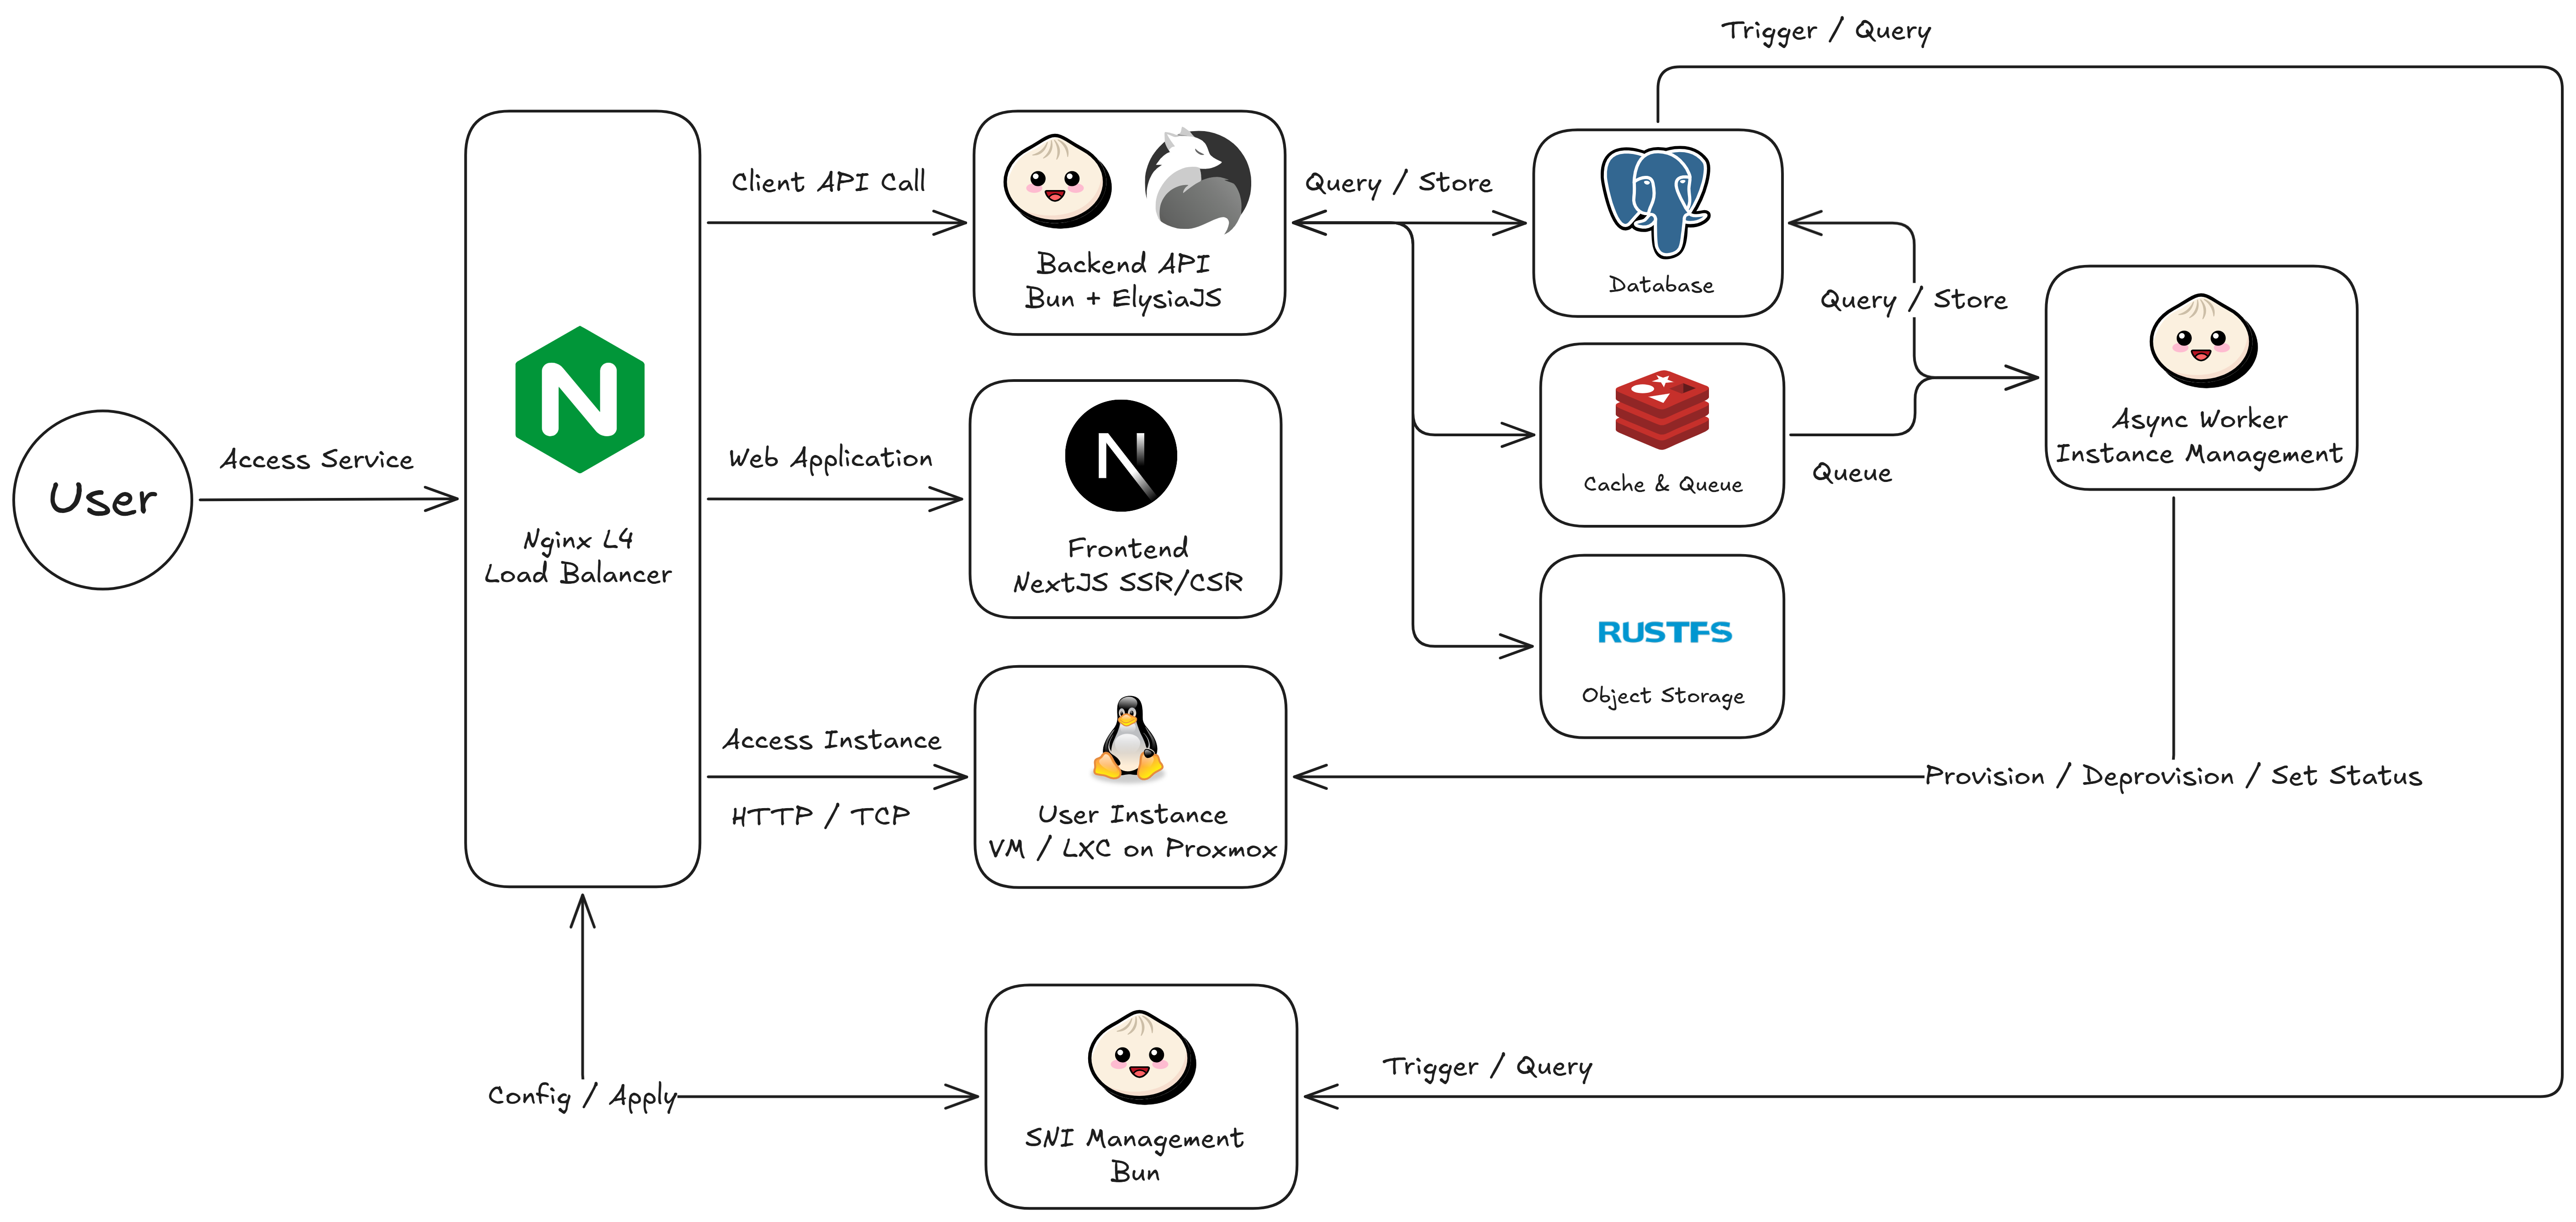
\includegraphics[width=1.0\linewidth]{Image/current_system_diagram.png}
    \caption{\fontSixTeen{แผนภาพการทํางานและลําดับขั้นตอนโดยรวมของโปรแกรม}}
    \label{fig3:system_overview_flow}
\end{figure}

\hspace*{1.3em} %ย่อหน้า
จากภาพที่ \ref{fig3:system_overview_flow} จะเห็นลำดับการทำงานหลักของแพลตฟอร์มอย่างเป็นขั้นตอน โดยผู้ใช้เริ่มต้นจากการเข้าใช้งานผ่าน Midori ซึ่งเป็นส่วนติดต่อผู้ใช้ จากนั้นคำขอจะถูกส่งต่อไปยัง Momoi เพื่อประมวลผลตรรกะทางธุรกิจ ตรวจสอบสิทธิ์ และบันทึกข้อมูลลงในฐานข้อมูล หากเป็นงานที่ต้องใช้เวลานานหรือเกี่ยวข้องกับการจัดสรรทรัพยากรเครื่องเสมือน Momoi จะส่งงานเข้าสู่คิวเพื่อให้ Yuzu รับไปดำเนินการกับ Proxmox VE แบบอะซิงโครนัส ขณะเดียวกันข้อมูลที่เกี่ยวข้องกับ reverse proxy และ SSH access จะถูก Satsuki ซึ่งติดตั้งอยู่บนเครื่อง Nginx ภายนอกนำไปสร้างไฟล์กำหนดค่าและ reload บริการหน้าด่านให้สอดคล้องกับสถานะล่าสุดของระบบ ภาพนี้จึงช่วยสรุปความสัมพันธ์ระหว่างบริการหลัก เส้นทางข้อมูล และจุดที่เกิดการประมวลผลเบื้องหลัง ก่อนจะลงรายละเอียดในแผนภาพบริบทและแผนภาพการไหลของข้อมูลระดับถัดไป

% แผนภาพนี้ควรรีเจนจากไฟล์ Mermaid: docs/diagram/chapter3-context-diagram.mmd
\begin{figure}[H]
    \centering
    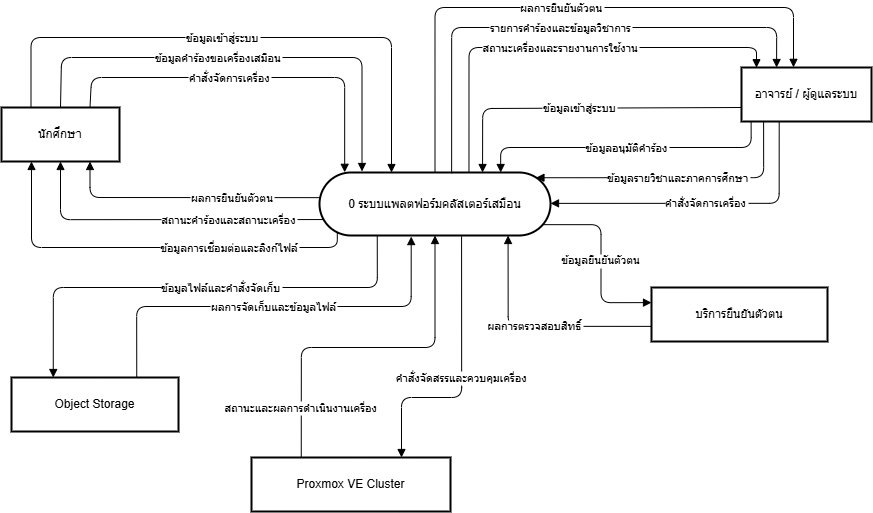
\includegraphics[width=1.0\linewidth]{Image/diagram/chapter3-context-diagram.png}
    \caption{\fontSixTeen{แผนภาพบริบทของระบบแพลตฟอร์มคลัสเตอร์เสมือน}}
    \label{fig3:context_diagram}
\end{figure}

\hspace*{1.3em} %ย่อหน้า
จากภาพที่ \ref{fig3:context_diagram} ระบบถูกมองเป็นกระบวนการเดียวในลักษณะ Black Box เพื่อแสดงเฉพาะความสัมพันธ์ระหว่างระบบกับเอนทิตีภายนอก ได้แก่ นักศึกษา อาจารย์หรือผู้ดูแลระบบ บริการยืนยันตัวตน Proxmox VE Cluster และ Object Storage โดยไม่มีการแสดงแหล่งเก็บข้อมูลภายในตามหลักของ Context Diagram จากนั้นในภาพที่ \ref{fig3:data_flow_level_0} ได้ทำการแตกกระบวนการหลักของระบบออกเป็น 5 กระบวนการ พร้อมเพิ่มแหล่งเก็บข้อมูลที่จำเป็น โดยแยกแสดงเป็น 3 มุมมองเพื่อความชัดเจน และในภาพที่ \ref{fig3:data_flow_level_1_auth} – \ref{fig3:data_flow_level_1_vm} ได้ขยายรายละเอียดทั้ง 5 กระบวนการหลัก เพื่อรักษาความสมดุลของกระแสข้อมูลระหว่างแต่ละระดับของ DFD ให้สอดคล้องกัน

% แผนภาพนี้ควรรีเจนจากไฟล์ Mermaid: docs/diagram/chapter3-dataflow-level0.mmd
\begin{figure}[H]
    \centering
    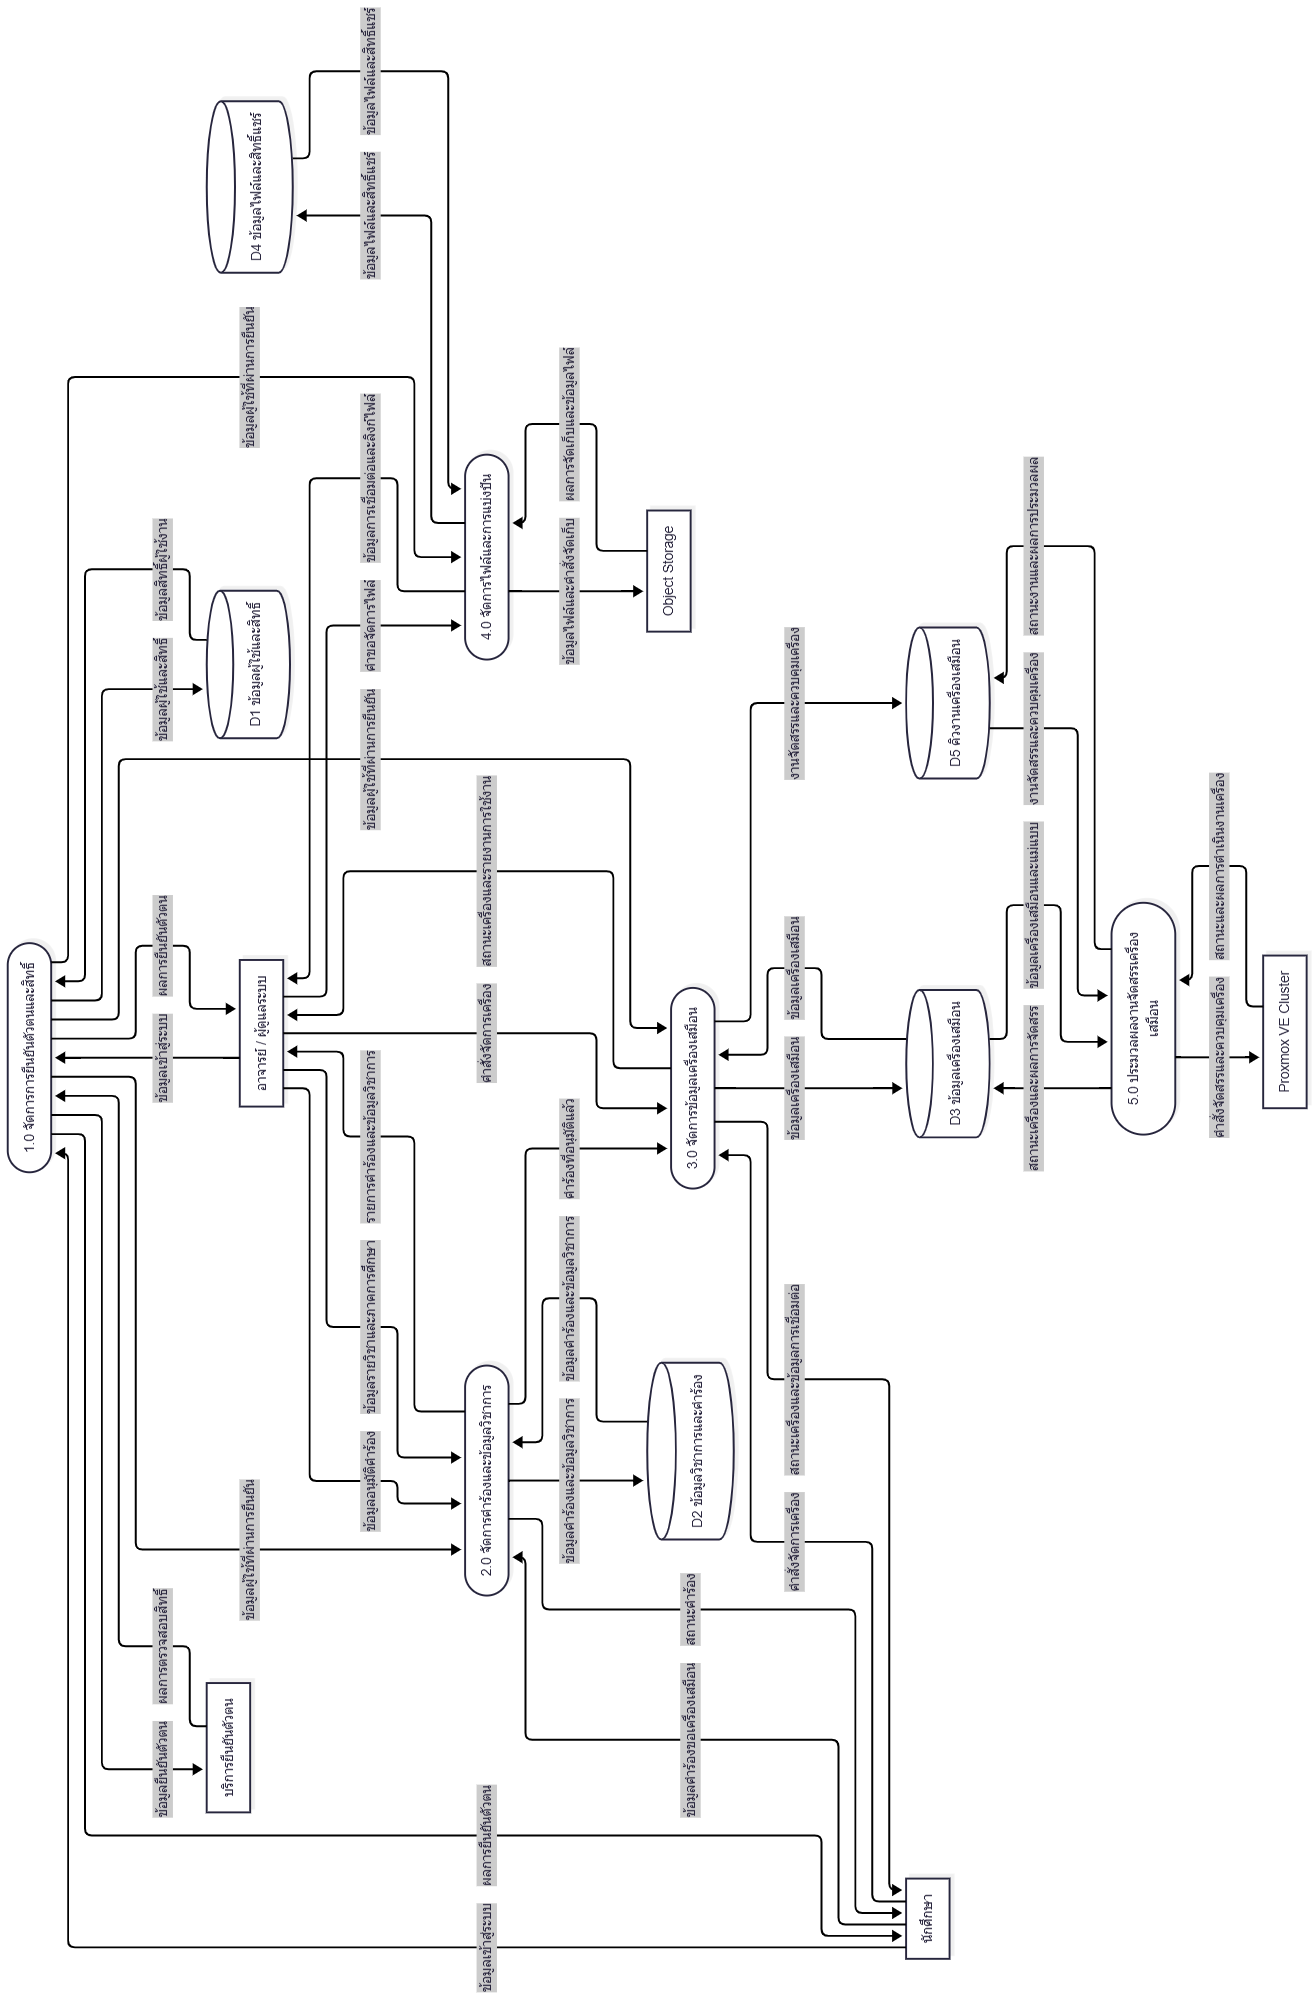
\includegraphics[width=1.0\textwidth]{Image/diagram/chapter3-dataflow-level0_90.png}
    \caption{\fontSixTeen{แผนภาพการไหลของข้อมูลระดับ 0: ภาพรวมทั้งระบบ}}
    \label{fig3:data_flow_level_0}
\end{figure}

% \begin{figure}[H]
%     \centering
%     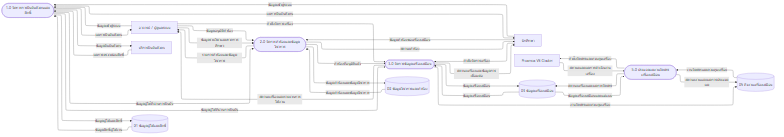
\includegraphics[width=1.0\textwidth]{Image/diagram/chapter3-dataflow-level0-vm-operations.png}
%     \caption{\fontSixTeen{แผนภาพการไหลของข้อมูลระดับ 0: กลุ่มกระบวนการจัดการคำร้องและเครื่องเสมือน}}
%     \label{fig3:data_flow_level_0_vm_operations}
% \end{figure}

% \begin{figure}[H]
%     \centering
%     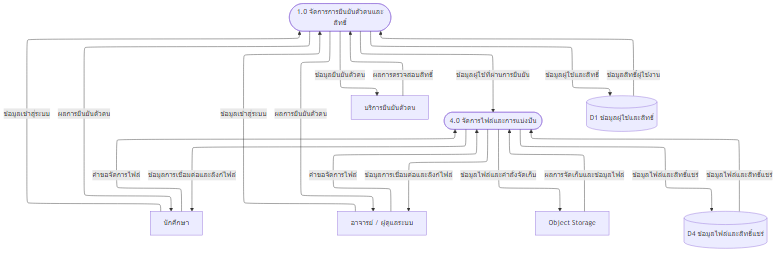
\includegraphics[width=1.0\textwidth]{Image/diagram/chapter3-dataflow-level0-storage.png}
%     \caption{\fontSixTeen{แผนภาพการไหลของข้อมูลระดับ 0: กลุ่มกระบวนการยืนยันตัวตนและจัดการไฟล์}}
%     \label{fig3:data_flow_level_0_storage}
% \end{figure}

\hspace*{1.3em} %ย่อหน้า
ในระดับแผนภาพการไหลของข้อมูลระดับที่ 1 (DFD Level 1) ตามภาพที่ \ref{fig3:data_flow_level_1_auth} – \ref{fig3:data_flow_level_1_vm} ได้ทำการขยายกระบวนการหลักจากระดับ 0 ให้เห็นรายละเอียดของกระแสข้อมูลภายในระบบมากขึ้น โดยยังคงรักษาหลัก \textit{Balancing} กล่าวคือ ข้อมูลเข้าและข้อมูลออกของแต่ละกระบวนการหลักต้องสอดคล้องกับสิ่งที่ปรากฏใน DFD ระดับ 0 และไม่สร้าง/ลบกระแสข้อมูลที่ไม่มีอยู่ในระดับก่อนหน้า ทั้งนี้สามารถสรุปแนวคิดสำคัญของกระบวนการระดับที่ 1 ได้ดังนี้

\begin{figure}[H]
    \centering
    % แผนภาพนี้ควรรีเจนจากไฟล์ Mermaid: docs/diagram/chapter3-dataflow-level1-process1.mmd
    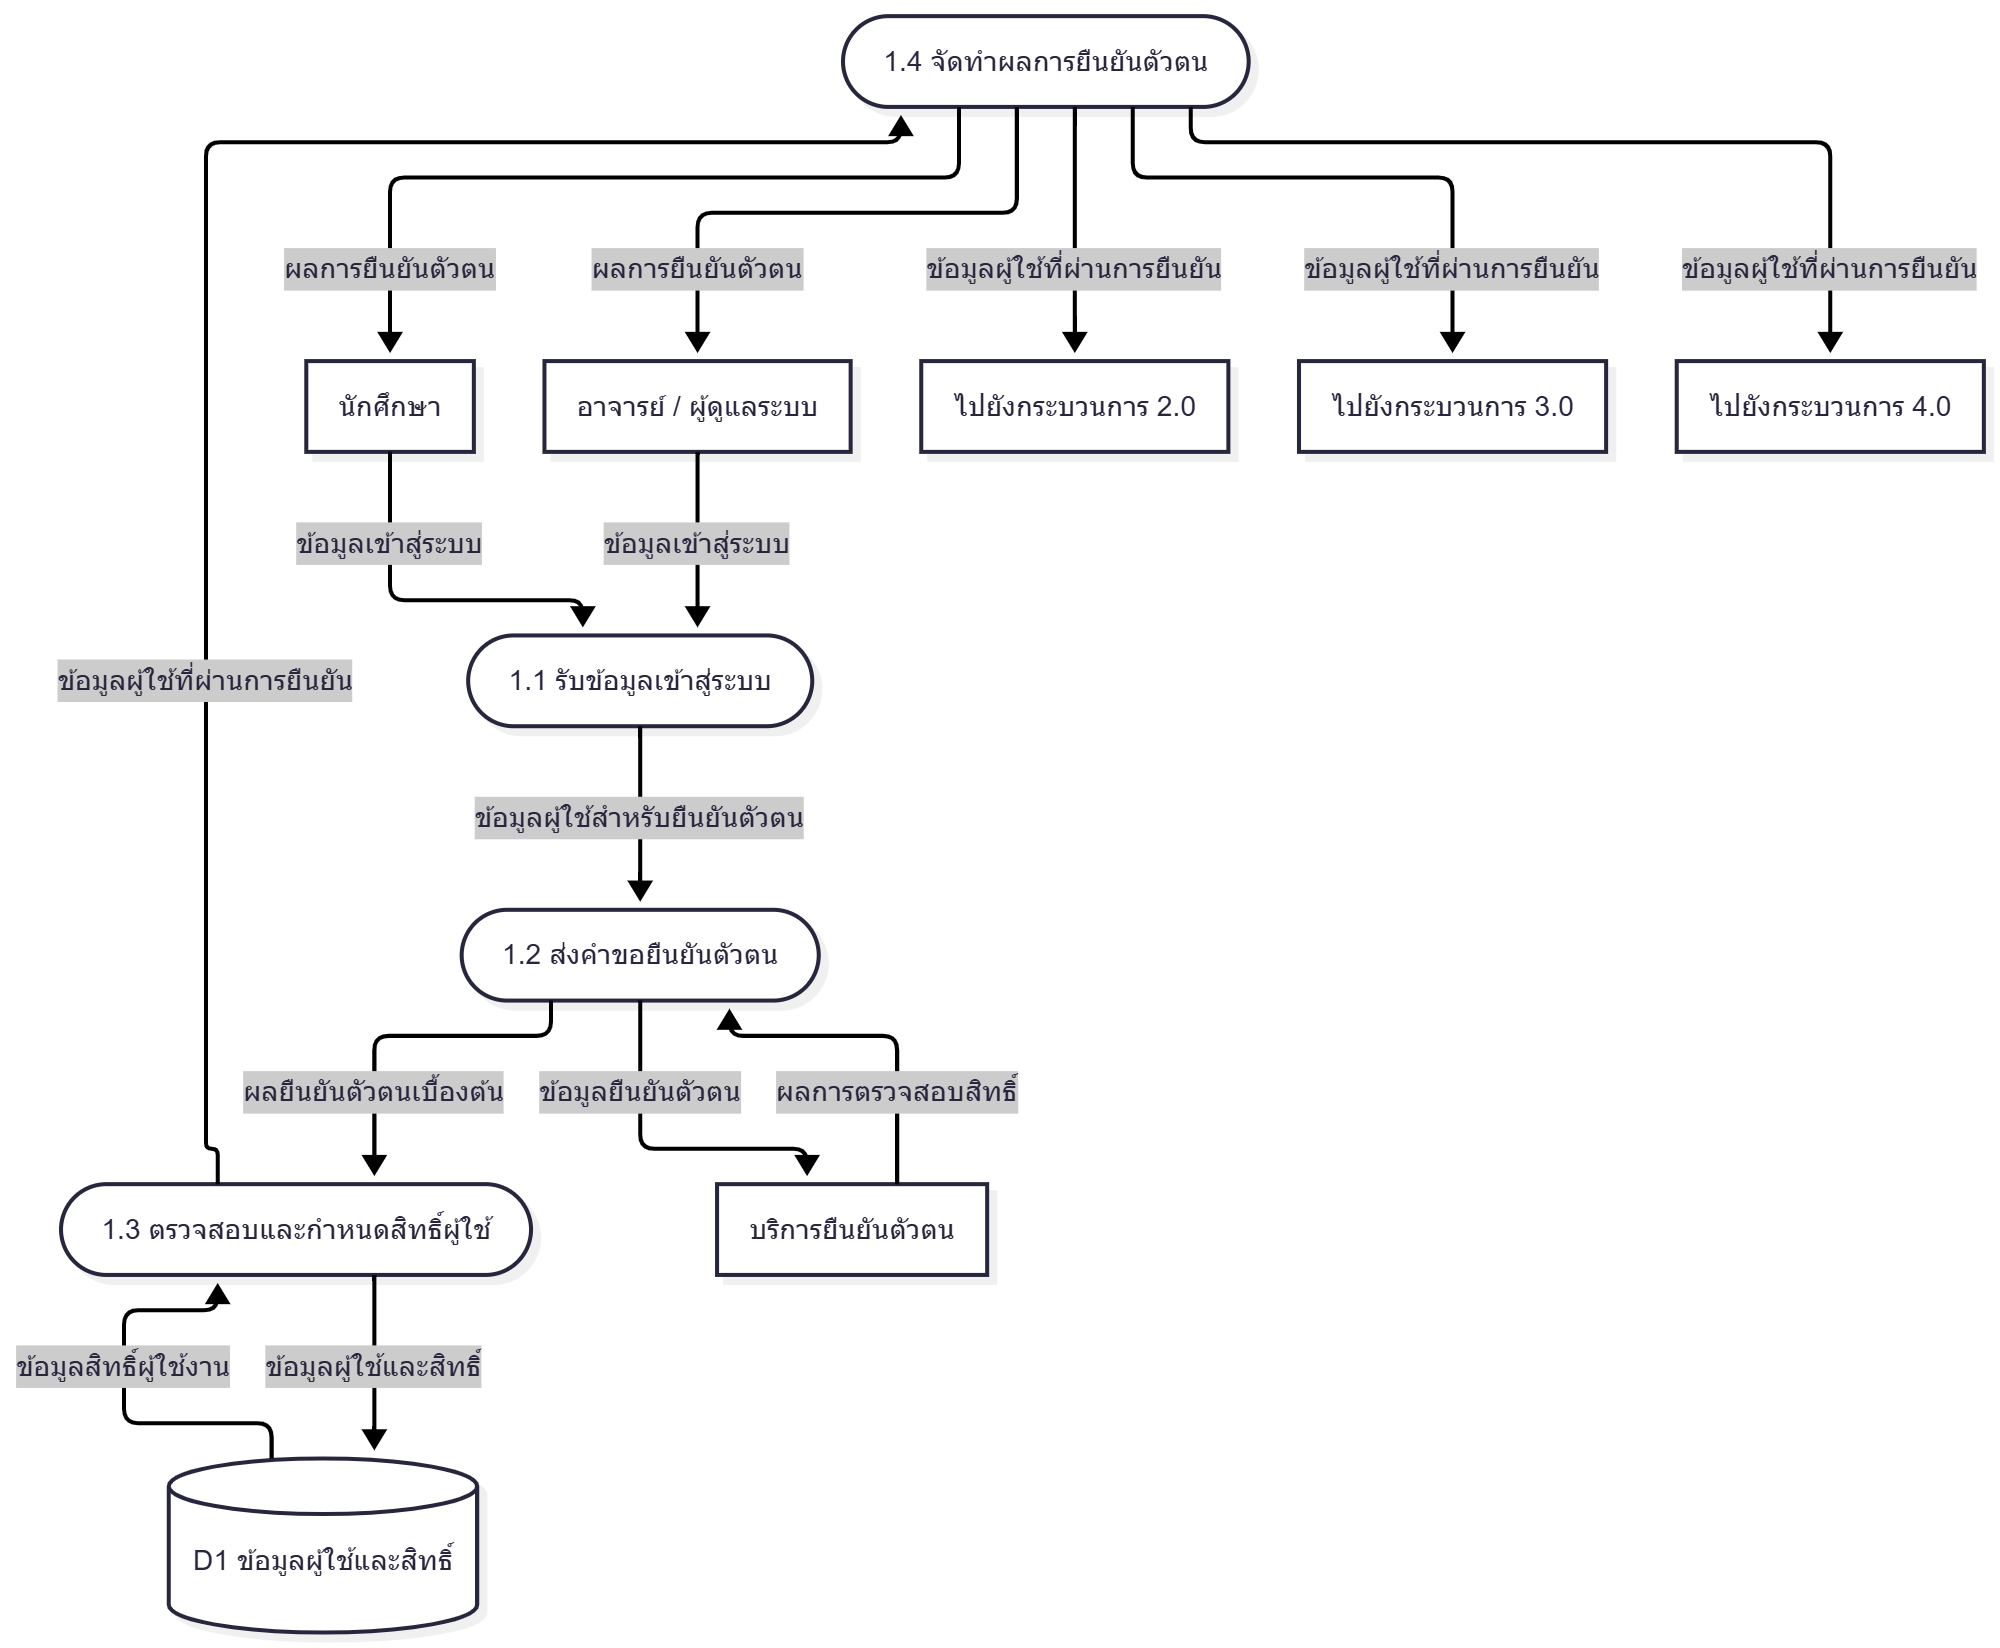
\includegraphics[width=1.0\textwidth]{Image/diagram/chapter3-dataflow-level1-process1.png}
    \caption{\fontSixTeen{แผนภาพการไหลของข้อมูลระดับที่ 1 ของกระบวนการ 1.0 การยืนยันตัวตนและกำหนดสิทธิ์ผู้ใช้}}
    \label{fig3:data_flow_level_1_auth}
\end{figure}

\hspace*{1.3em} %ย่อหน้า
\textbf{กระบวนการ 1.0 การยืนยันตัวตนและกำหนดสิทธิ์ผู้ใช้} (ภาพที่ \ref{fig3:data_flow_level_1_auth}) ทำหน้าที่เป็น \textit{gatekeeper} ของ API ทั้งระบบ โดยรับข้อมูลยืนยันตัวตนจากผู้ใช้ผ่าน Midori จากนั้นสร้าง/ตรวจสอบ Session และผูกกับข้อมูลผู้ใช้ในฐานข้อมูลเพื่อกำหนดบทบาท (ADMIN/INSTRUCTOR/STUDENT) เส้นทางนี้ให้บริการผ่านโมดูล better-auth ภายใน Momoi และใช้ฐานข้อมูลพร้อมกติกา RBAC ชุดเดียวกับบริการ API อื่น ๆ ผลลัพธ์คือ token/session ที่ใช้ซ้ำได้ในการเรียก API อื่น ๆ และข้อมูลสิทธิ์ที่ใช้ประกอบการอนุมัติการเข้าถึงทรัพยากร

\begin{figure}[H]
    \centering
    % แผนภาพนี้ควรรีเจนจากไฟล์ Mermaid: docs/diagram/chapter3-dataflow-level1-process2.mmd
    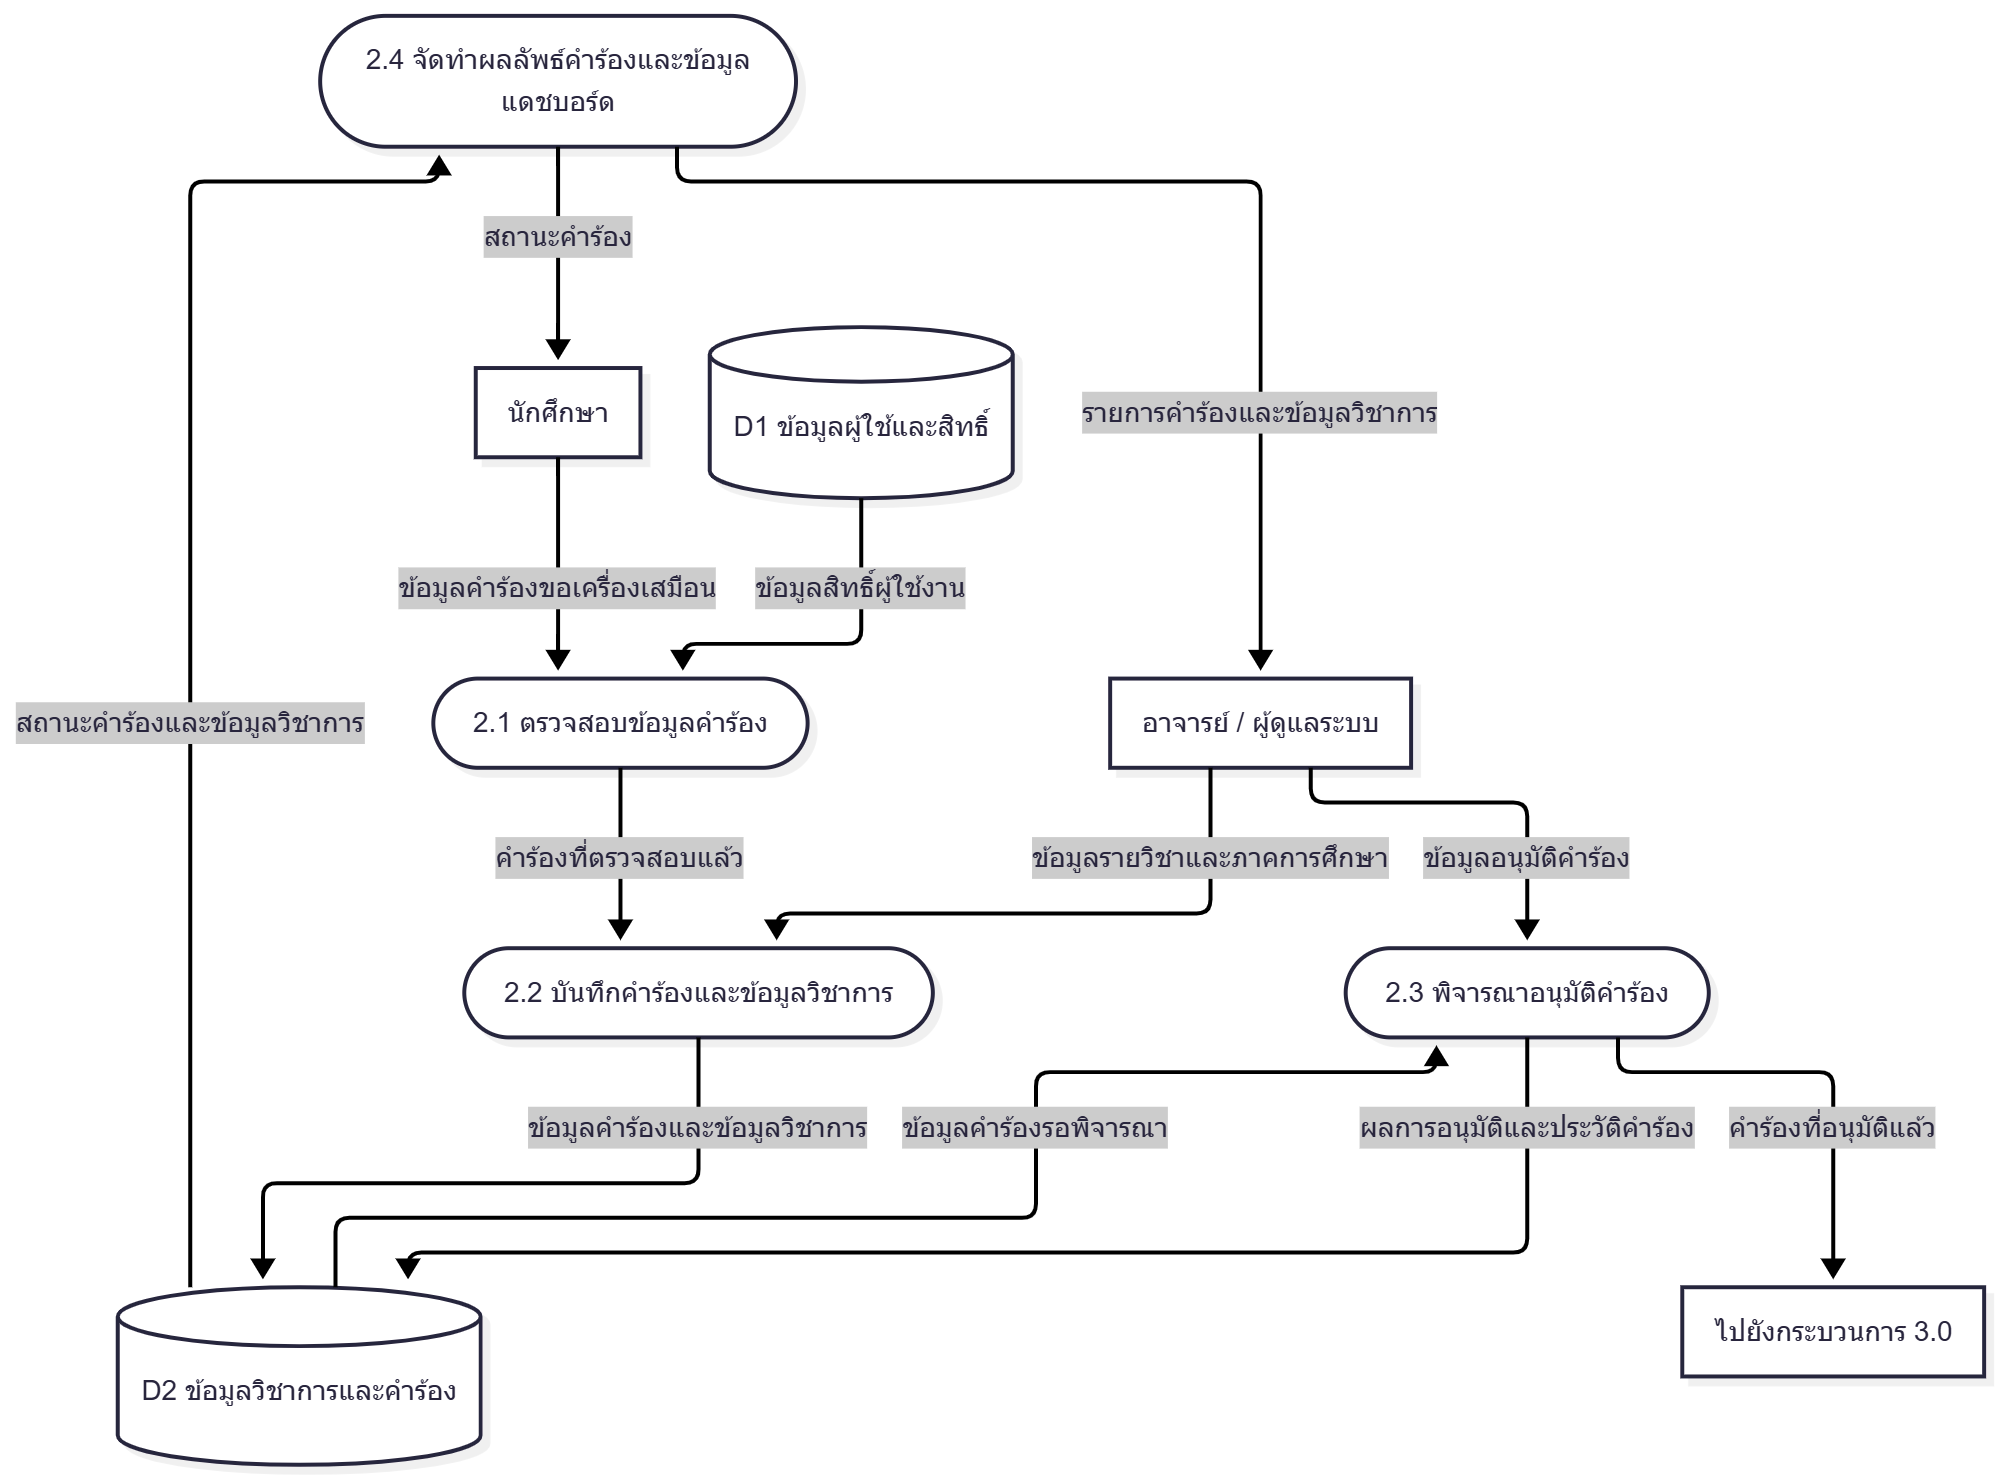
\includegraphics[width=1.0\textwidth]{Image/diagram/chapter3-dataflow-level1-process2.png}
    \caption{\fontSixTeen{แผนภาพการไหลของข้อมูลระดับที่ 1 ของกระบวนการ 2.0 การจัดการคำร้องและข้อมูลวิชาการ}}
    \label{fig3:data_flow_level_1_frontend}
\end{figure}

\hspace*{1.3em} %ย่อหน้า
\textbf{กระบวนการ 2.0 การจัดการคำร้องและข้อมูลวิชาการ} (ภาพที่ \ref{fig3:data_flow_level_1_frontend}) เน้นการจัดการข้อมูลเชิงโดเมนที่เกี่ยวข้องกับผู้ใช้และการเรียนการสอน เช่น รายวิชา/ภาคการศึกษา/ผู้สอน รวมถึงวงจรคำร้องขอเครื่องเสมือนและการตรวจสอบสิทธิ์ของผู้ยื่นคำร้อง จุดสำคัญคือข้อมูลคำร้องและประวัติการอนุมัติจะถูกจัดเก็บแบบเป็นโครงสร้างเพื่อให้สามารถตรวจสอบย้อนหลังได้ และสถานะคำร้องถูกส่งกลับไปยัง UI เพื่อสื่อสารความคืบหน้าให้ผู้ใช้

\begin{figure}[H]
    \centering
    % แผนภาพนี้ควรรีเจนจากไฟล์ Mermaid: docs/diagram/chapter3-dataflow-level1-process3.mmd
    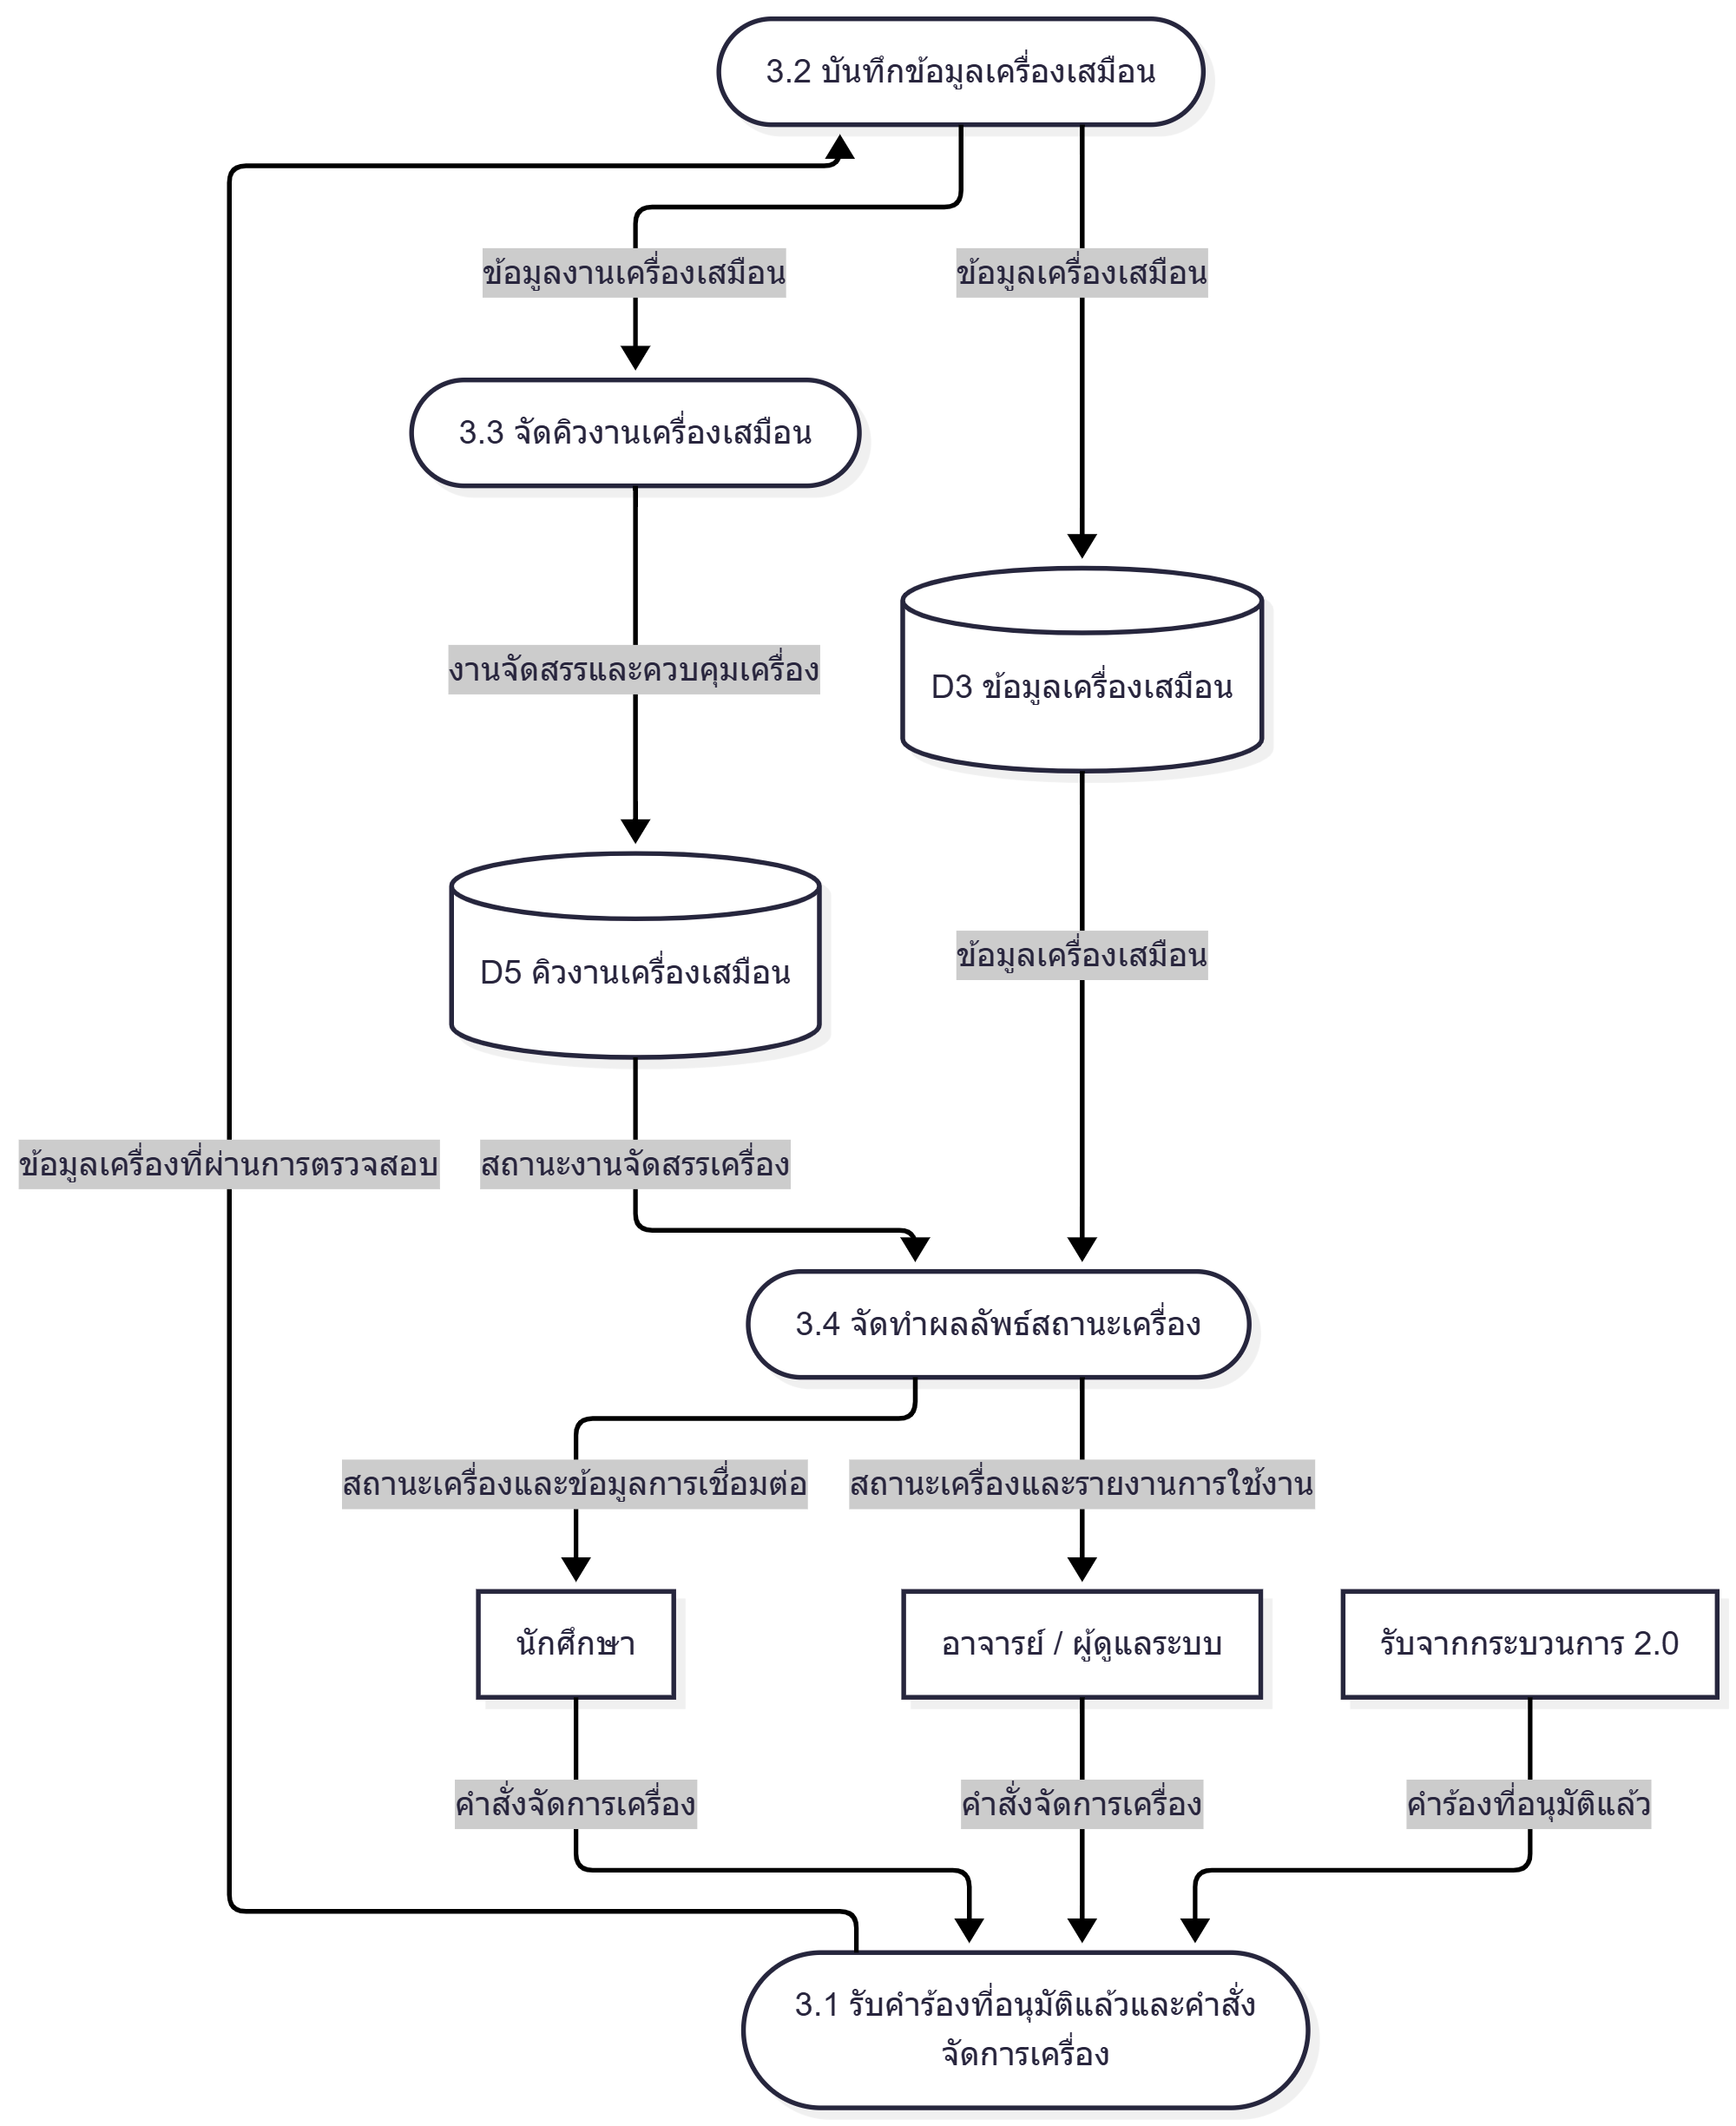
\includegraphics[width=0.95\textwidth]{Image/diagram/chapter3-dataflow-level1-process3.png}
    \caption{\fontSixTeen{แผนภาพการไหลของข้อมูลระดับที่ 1 ของกระบวนการ 3.0 การจัดการข้อมูลเครื่องเสมือน}}
    \label{fig3:data_flow_level_1_backend}
\end{figure}

\hspace*{1.3em} %ย่อหน้า
\textbf{กระบวนการ 3.0 การจัดการข้อมูลเครื่องเสมือน} (ภาพที่ \ref{fig3:data_flow_level_1_backend}) เป็นส่วนกลางของการจัดการ VM ในเชิงธุรกรรม โดยอ่าน/เขียนข้อมูล Instance และความสัมพันธ์กับทรัพยากร Proxmox VE ในฐานข้อมูล รวมถึงการตัดสินใจว่างานใดควรประมวลผลแบบทันที (เช่นการอ่านสถานะจากฐานข้อมูล) และงานใดควรส่งไปประมวลผลแบบอะซิงโครนัสผ่านคิว (เช่นการสร้าง/ลบ/สั่งเริ่ม-หยุด VM) เพื่อให้ API ตอบสนองรวดเร็วและรองรับการ retry ได้อย่างปลอดภัย

\begin{figure}[H]
    \centering
    % แผนภาพนี้ควรรีเจนจากไฟล์ Mermaid: docs/diagram/chapter3-dataflow-level1-process4.mmd
    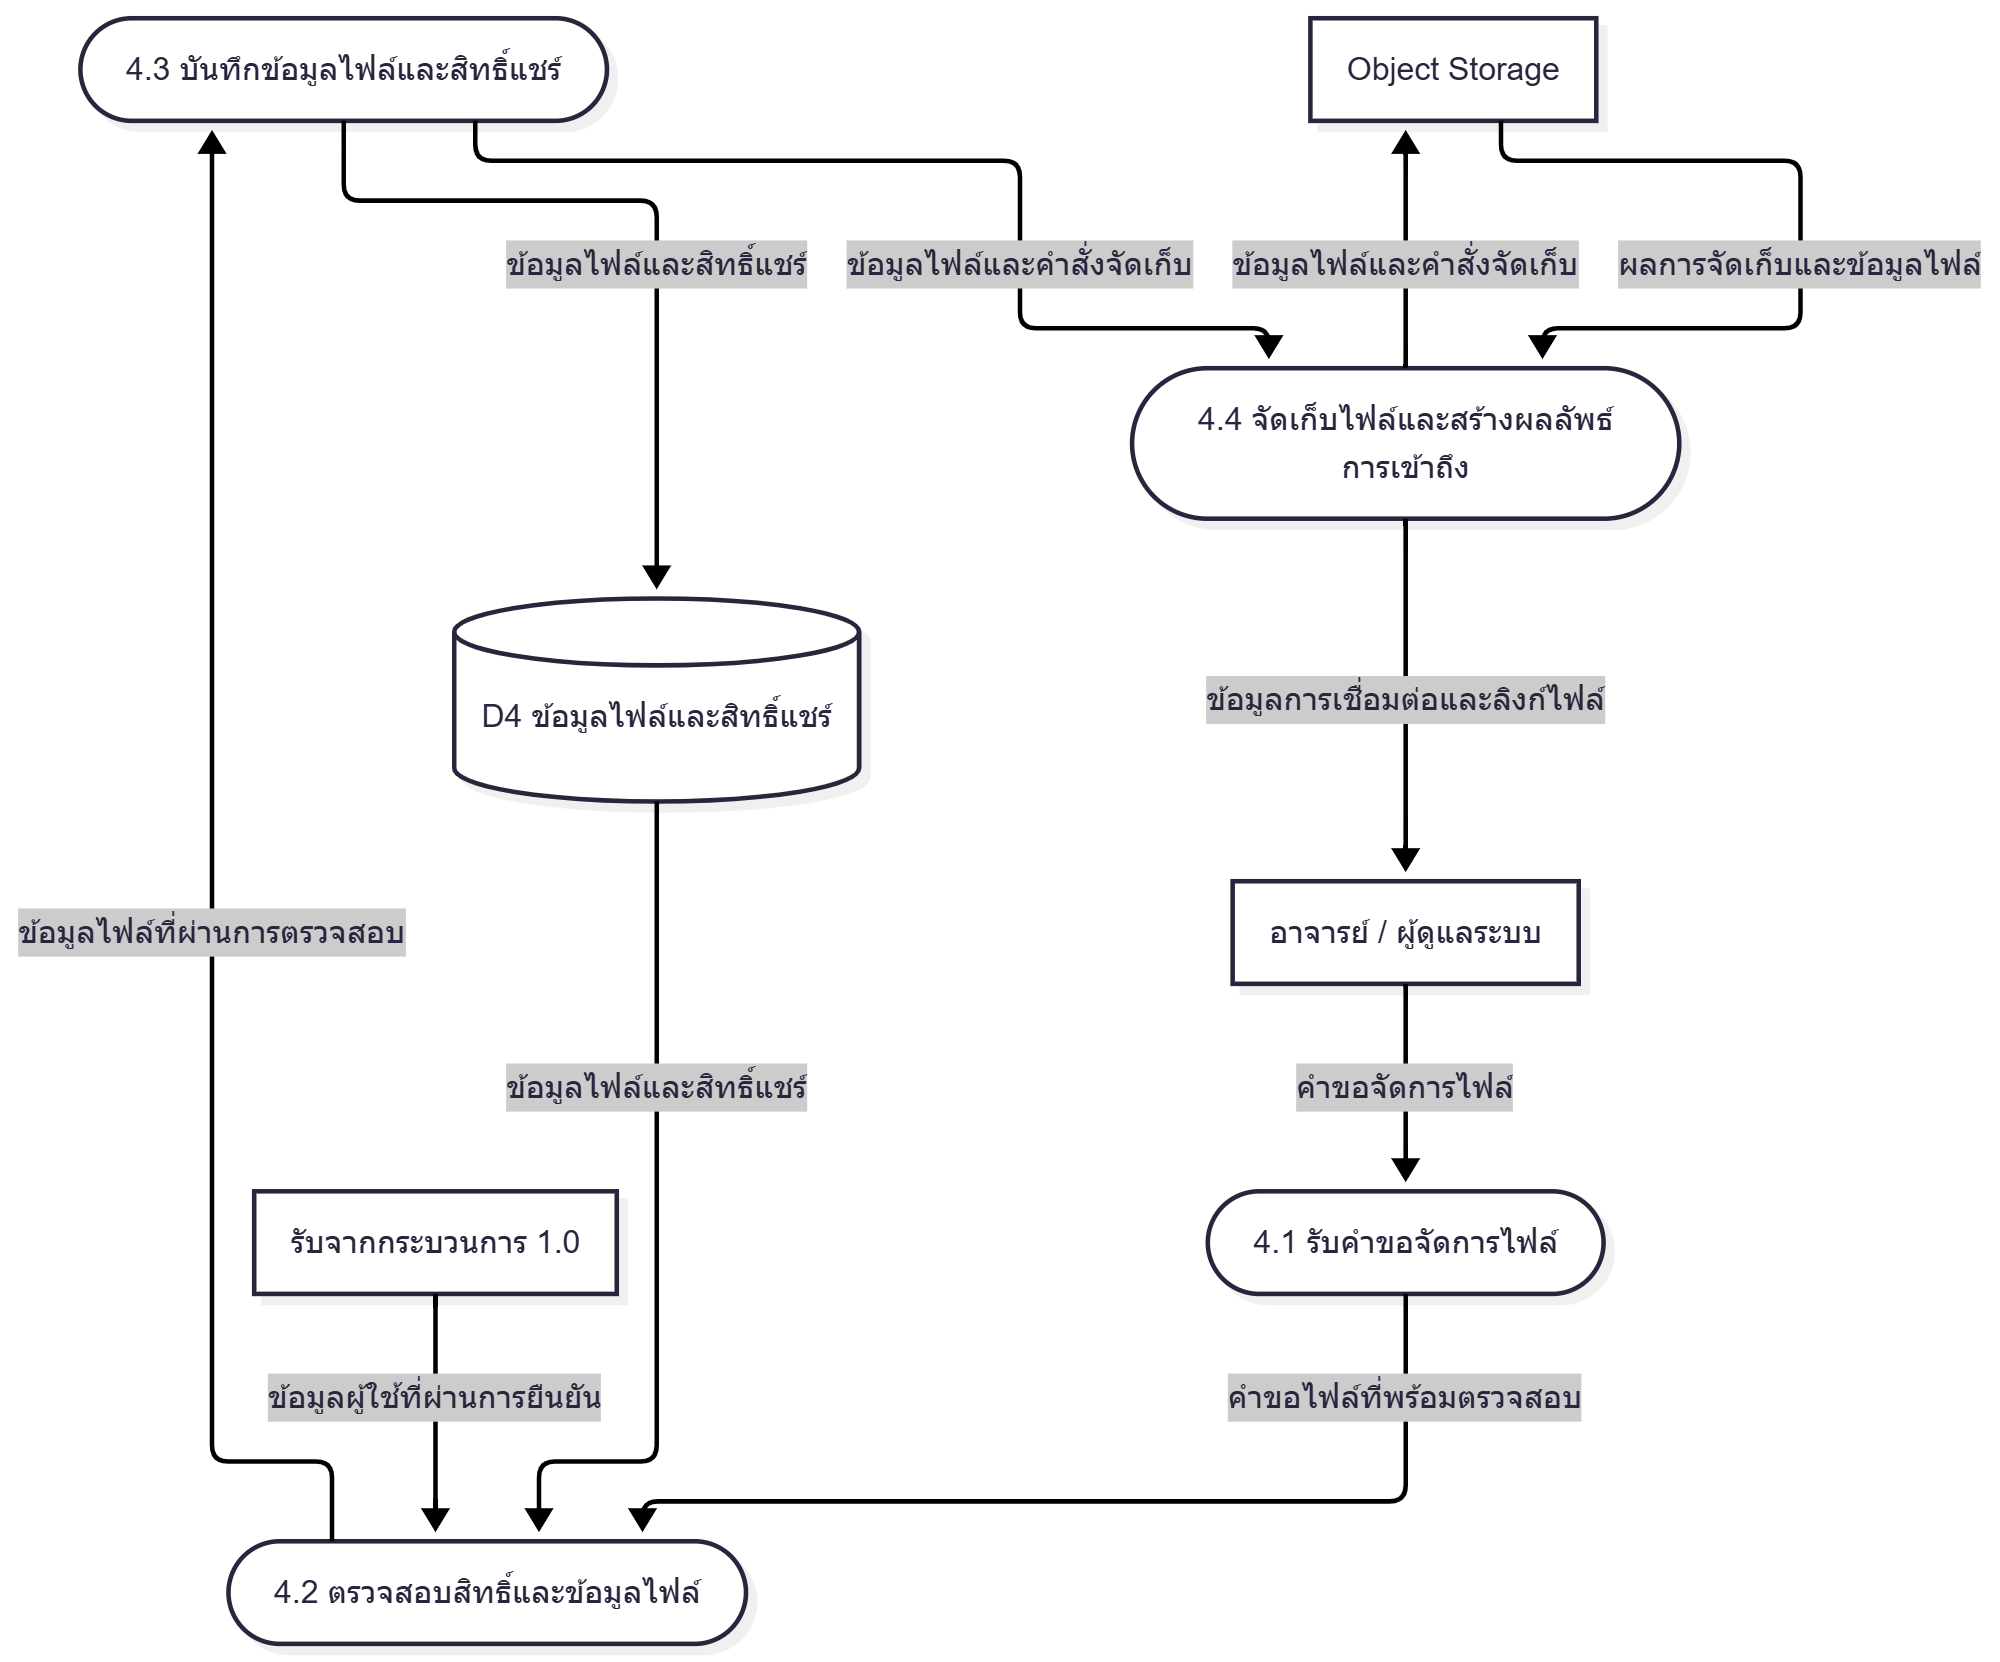
\includegraphics[width=1.0\textwidth]{Image/diagram/chapter3-dataflow-level1-process4.png}
    \caption{\fontSixTeen{แผนภาพการไหลของข้อมูลระดับที่ 1 ของกระบวนการ 4.0 การจัดการไฟล์และสิทธิ์การเข้าถึง}}
    \label{fig3:data_flow_level_1_storage}
\end{figure}

\hspace*{1.3em} %ย่อหน้า
\textbf{กระบวนการ 4.0 การจัดการไฟล์และสิทธิ์การเข้าถึง} (ภาพที่ \ref{fig3:data_flow_level_1_storage}) แยกการจัดการ \textit{เมทาดาทา} (เช่นชื่อไฟล์, owner, permission, เวลาอัปโหลด) ออกจาก \textit{ข้อมูลไฟล์จริง} ที่อยู่ใน Object Storage โดยกระบวนการนี้จึงต้องจัดการทั้งสิทธิ์เข้าถึงและการออกลิงก์/โทเคนการเข้าถึงตามนโยบายของระบบ เพื่อให้การควบคุมสิทธิ์สอดคล้องกับบทบาทผู้ใช้และบริบทของรายวิชา/คำร้อง

\begin{figure}[H]
    \centering
    % แผนภาพนี้ควรรีเจนจากไฟล์ Mermaid: docs/diagram/chapter3-dataflow-level1-process5.mmd
    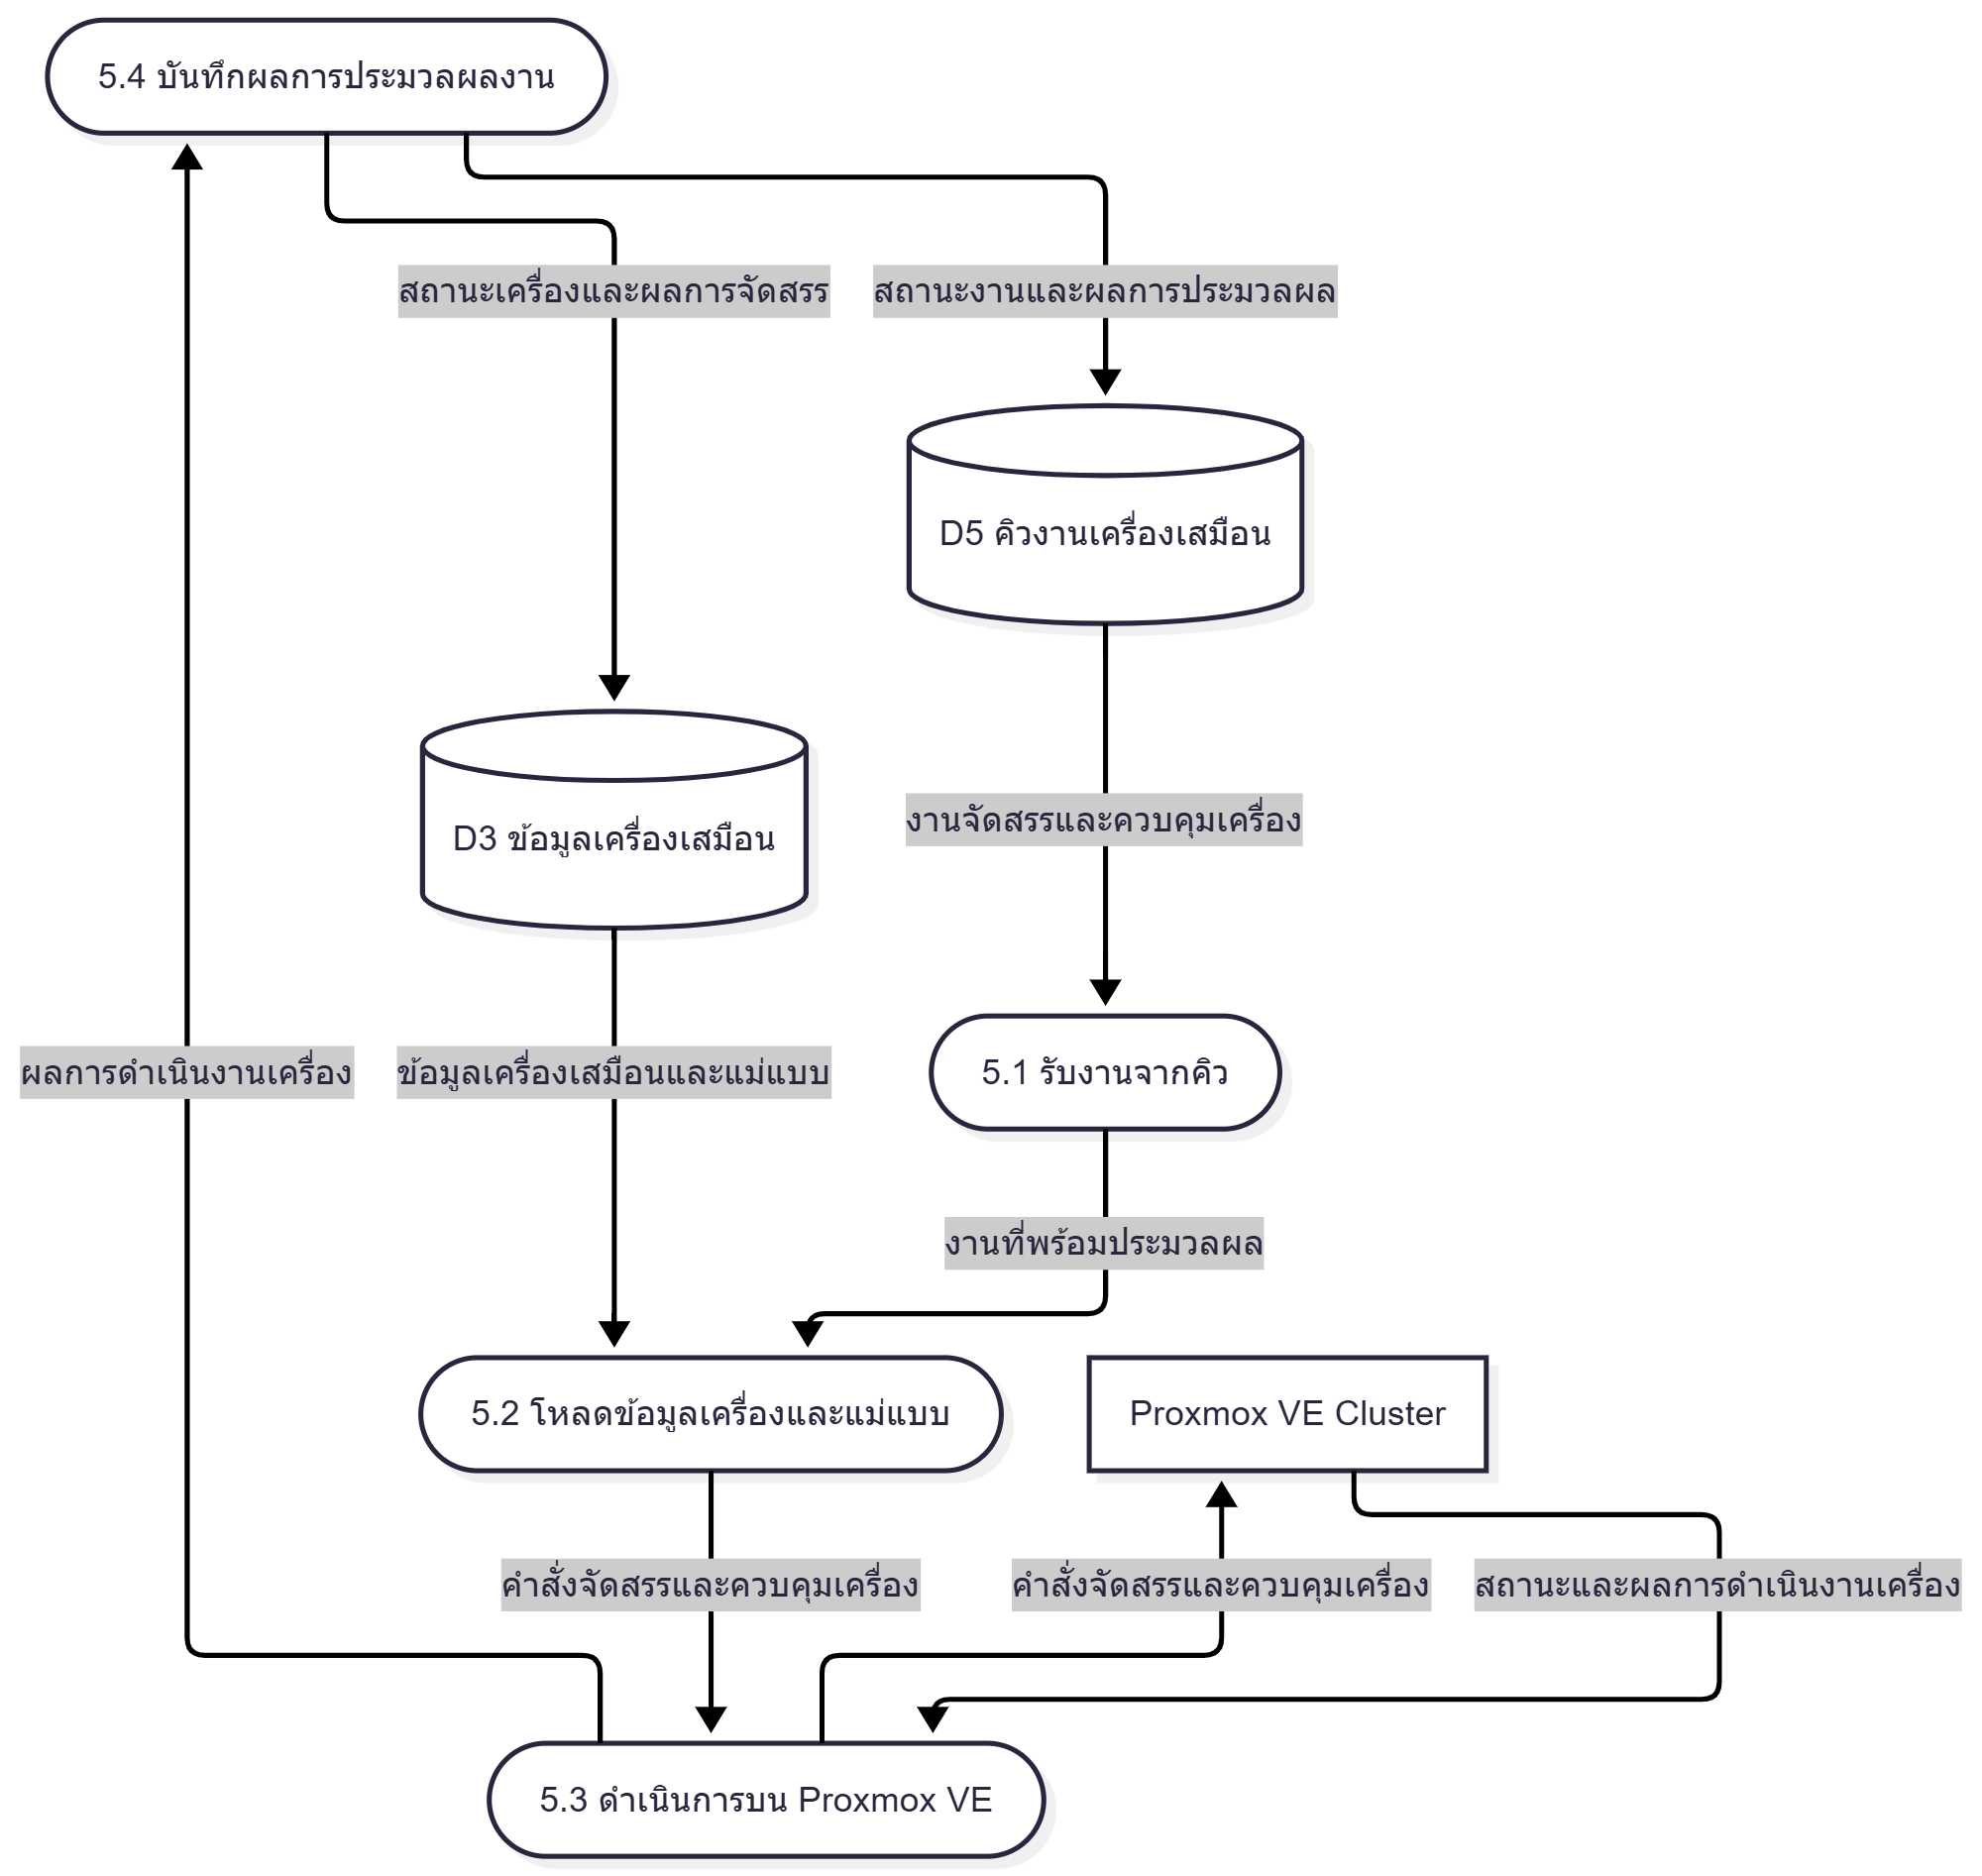
\includegraphics[width=1.0\textwidth]{Image/diagram/chapter3-dataflow-level1-process5.png}
    \caption{\fontSixTeen{แผนภาพการไหลของข้อมูลระดับที่ 1 ของกระบวนการ 5.0 การประมวลผลงานจัดสรรเครื่องเสมือน}}
    \label{fig3:data_flow_level_1_vm}
\end{figure}

\hspace*{1.3em} %ย่อหน้า
\textbf{กระบวนการ 5.0 การประมวลผลงานจัดสรรเครื่องเสมือน} (ภาพที่ \ref{fig3:data_flow_level_1_vm}) แสดงบทบาทของ worker (Yuzu) ในการรับงานจากคิวและเรียก Proxmox VE จริง โดยผลลัพธ์ที่ได้จาก Proxmox VE (สำเร็จ/ล้มเหลว/สถานะระหว่างทาง) จะถูกนำกลับมาอัปเดตฐานข้อมูล เพื่อให้ Midori และ Momoi แสดงสถานะล่าสุดแก่ผู้ใช้ได้จากแหล่งข้อมูลเดียวกัน (single source of truth)

\hspace*{1.3em} %ย่อหน้า
สำหรับการวิเคราะห์เชิงลึกเพิ่มเติม ได้จัดทำแผนภาพการไหลของข้อมูลระดับที่ 2 เพื่อขยายกระบวนการย่อยที่มีความซับซ้อน ได้แก่ การพิจารณาอนุมัติคำร้องในกระบวนการ 2.3 การรับคำร้องที่อนุมัติแล้วและจัดเตรียมงานในกระบวนการ 3.1 การส่งงานเข้าคิวในกระบวนการ 3.3 และการดำเนินการบน Proxmox VE ในกระบวนการ 5.3 ทั้งนี้การกำหนดชื่อกระแสข้อมูลในแต่ละระดับถูกจัดให้สอดคล้องกันตามหลัก Balancing ของ DFD ดังแสดงในภาพที่ \ref{fig3:data_flow_level_2_approval} – \ref{fig3:data_flow_level_2_pve}

\hspace*{1.3em} %ย่อหน้า
ในระดับ DFD Level 2 การขยายรายละเอียดมีเป้าหมายเพื่อทำให้เห็น \textbf{จุดตัดสินใจ (decision points)} และ \textbf{จุดที่ต้องรักษาความถูกต้องของข้อมูล (consistency points)} ของระบบอย่างชัดเจน โดยเฉพาะกระบวนการที่เกี่ยวข้องกับการอนุมัติ (ต้องตรวจสอบสิทธิ์และบันทึกประวัติ) และกระบวนการที่เกี่ยวข้องกับงานระยะยาว (ต้องส่งเข้าคิวและรองรับการ retry) ซึ่งสามารถอธิบายกลไกสำคัญได้ดังนี้

\begin{figure}[H]
    \centering
    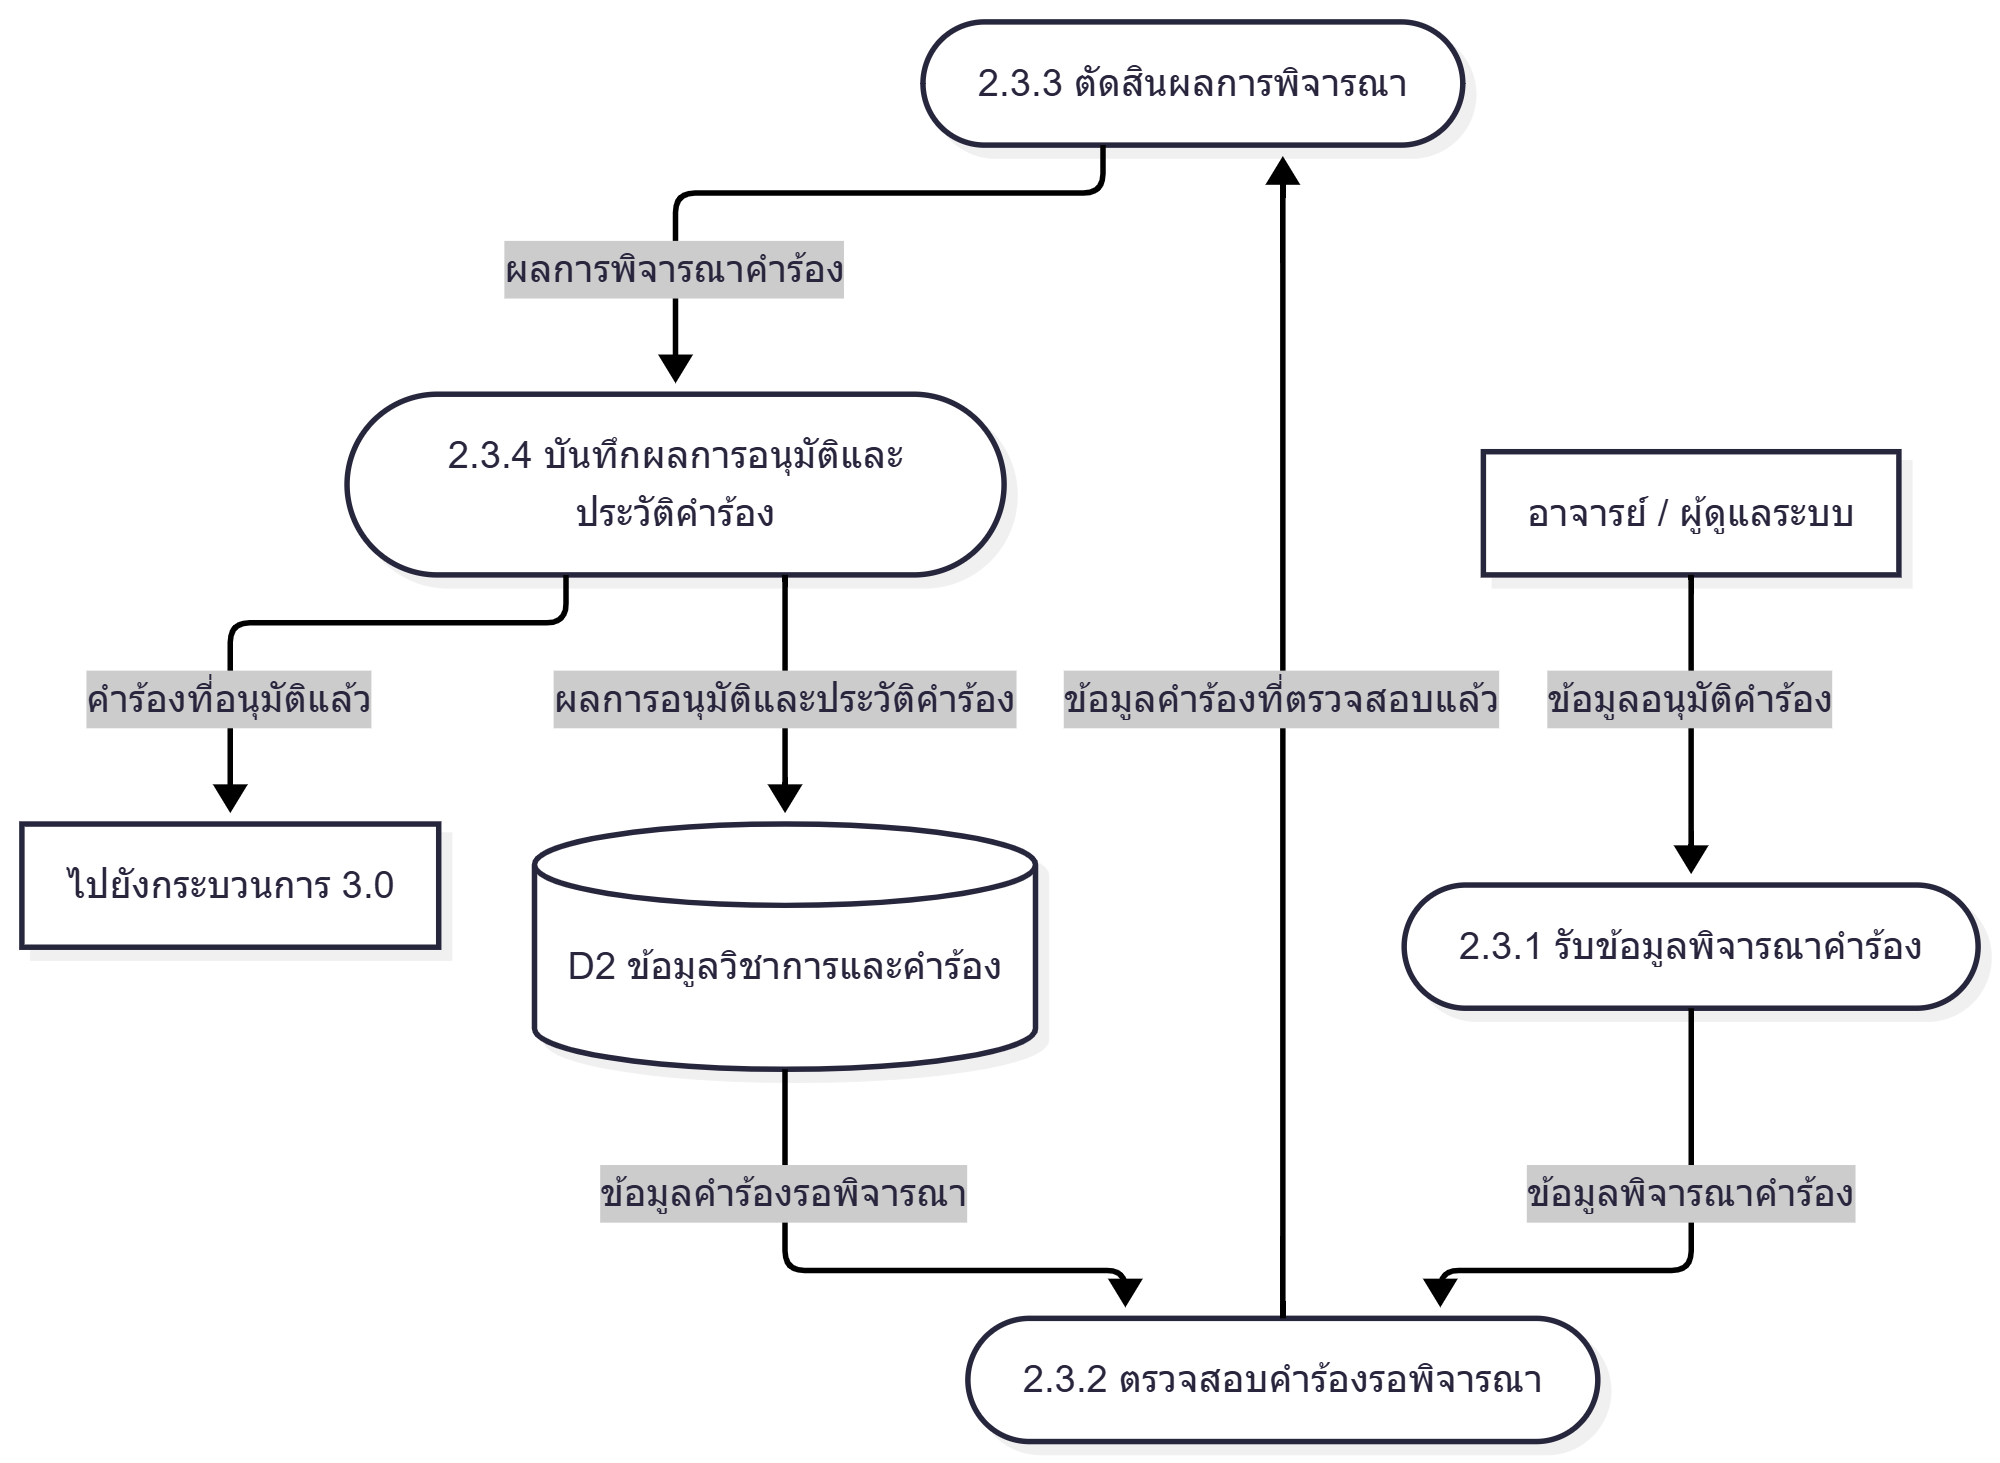
\includegraphics[width=1.0\textwidth]{Image/diagram/chapter3-dataflow-level2-process2-3.png}
    \caption{\fontSixTeen{แผนภาพการไหลของข้อมูลระดับที่ 2 ของกระบวนการ 2.3 การพิจารณาอนุมัติคำร้อง}}
    \label{fig3:data_flow_level_2_approval}
\end{figure}

\hspace*{1.3em} %ย่อหน้า
\textbf{กระบวนการ 2.3 การพิจารณาอนุมัติคำร้อง} (ภาพที่ \ref{fig3:data_flow_level_2_approval}) เริ่มจากผู้ดูแลระบบ/อาจารย์ส่งคำสั่งอนุมัติหรือปฏิเสธคำร้อง ระบบจะตรวจสอบสิทธิ์ของผู้ดำเนินการและสถานะคำร้องปัจจุบันก่อน (เพื่อป้องกันการอนุมัติซ้ำหรืออนุมัติคำร้องที่ถูกยกเลิกแล้ว) จากนั้นจึงอัปเดตสถานะคำร้องในฐานข้อมูล พร้อมบันทึกประวัติการตัดสินใจลงในตาราง audit log เพื่อใช้ตรวจสอบย้อนหลัง และส่งผลลัพธ์/สถานะใหม่กลับไปยัง UI

\begin{figure}[H]
    \centering
    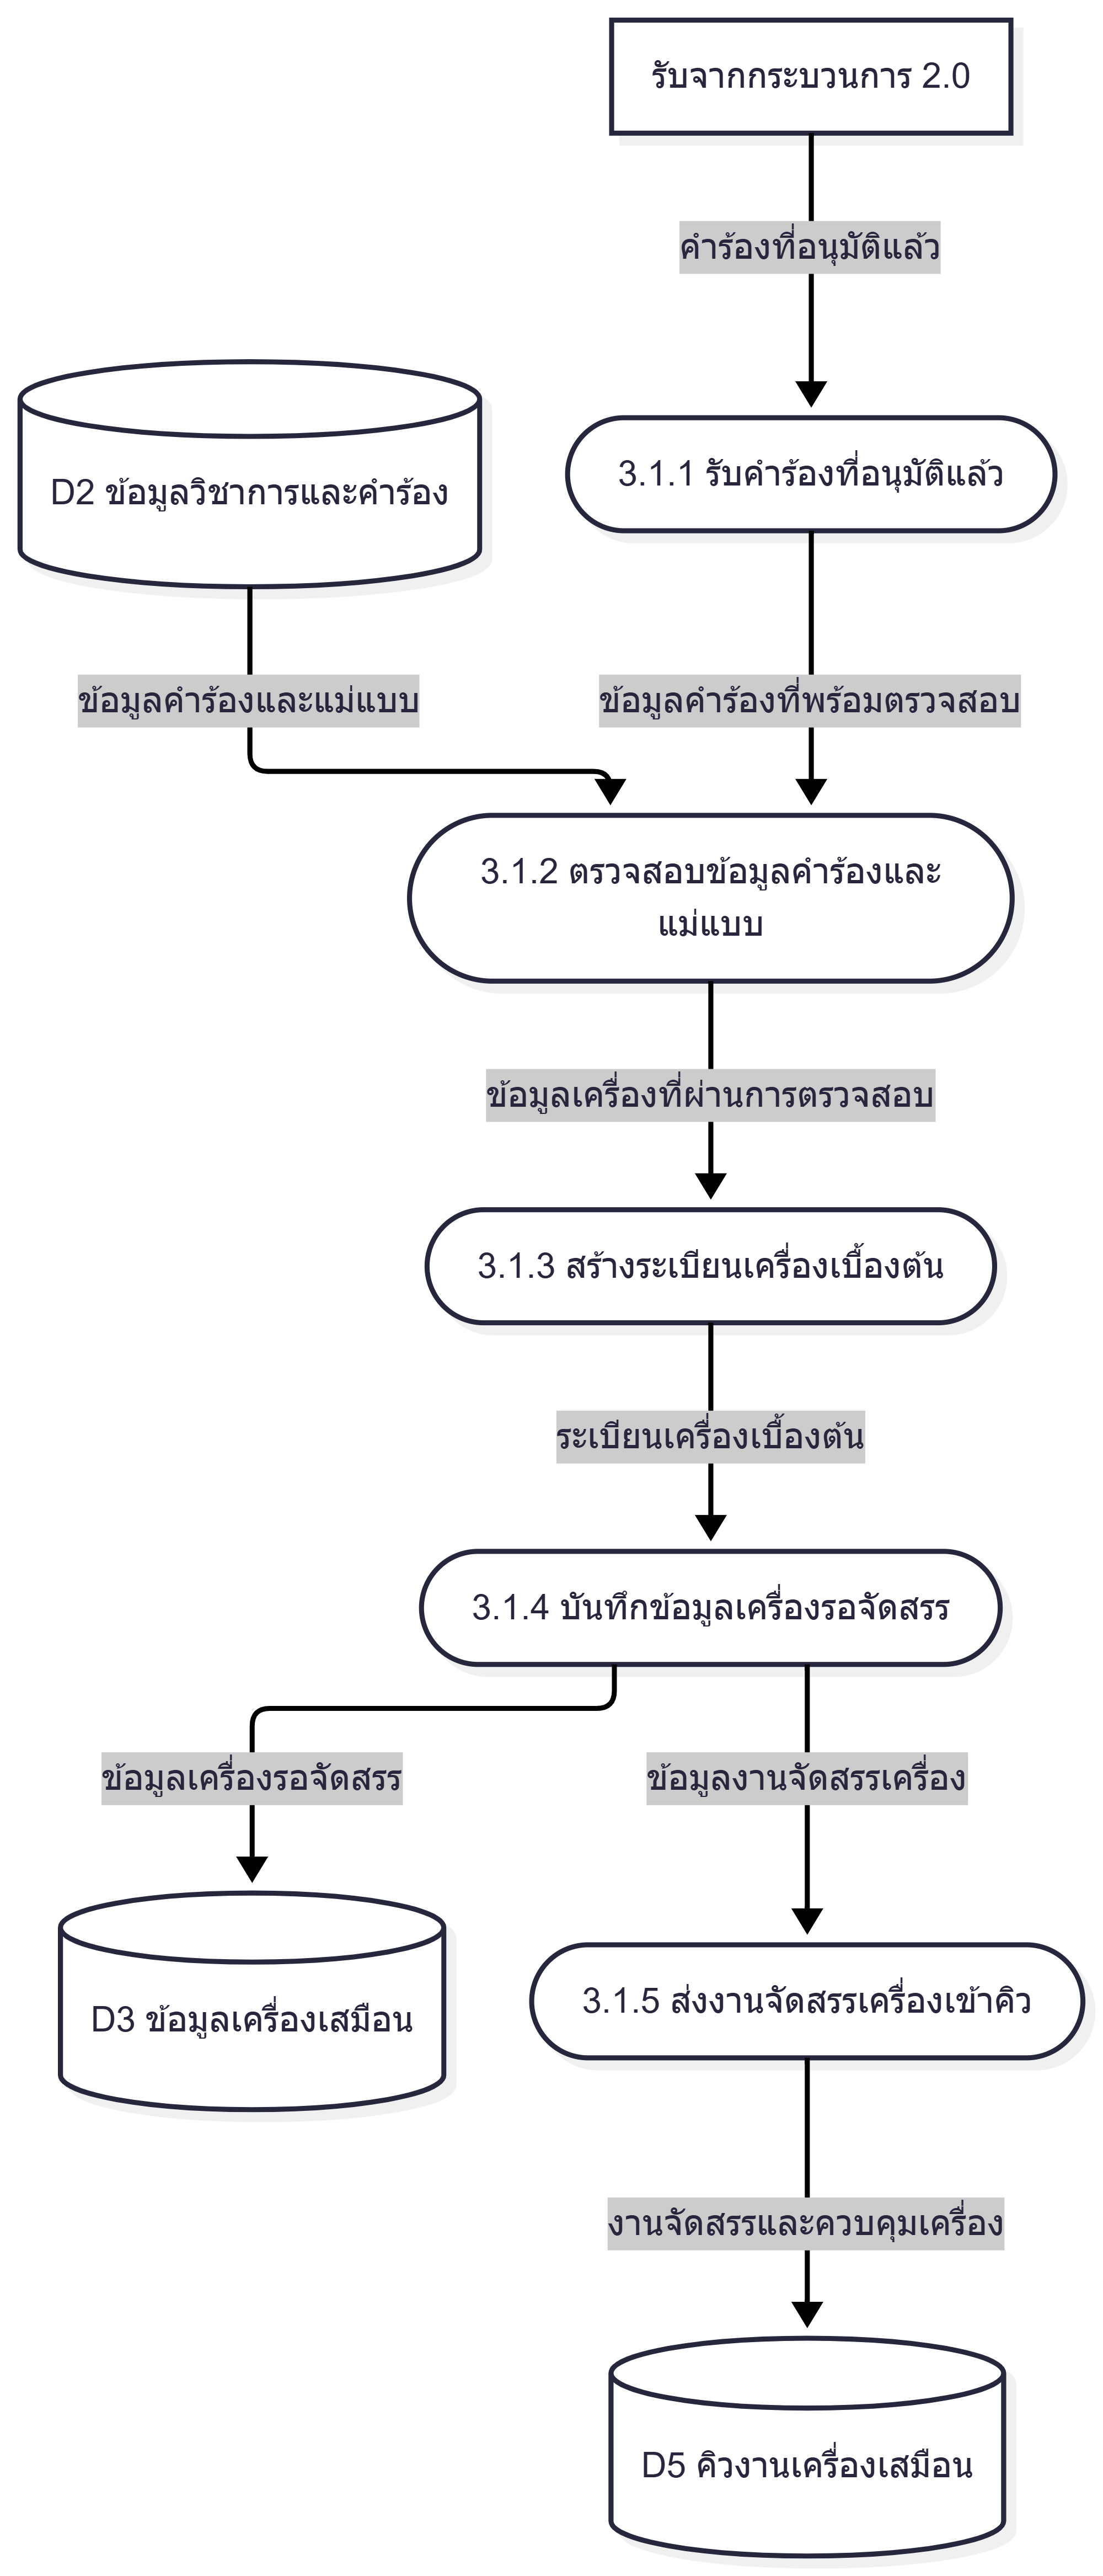
\includegraphics[width=0.50\textwidth]{Image/diagram/chapter3-dataflow-level2-process3-1.png}
    \caption{\fontSixTeen{แผนภาพการไหลของข้อมูลระดับที่ 2 ของกระบวนการ 3.1 การรับคำร้องที่อนุมัติแล้วและจัดเตรียมงาน}}
    \label{fig3:data_flow_level_2_provision}
\end{figure}

\hspace*{1.3em} %ย่อหน้า
\textbf{กระบวนการ 3.1 การรับคำร้องที่อนุมัติแล้วและจัดเตรียมงาน} (ภาพที่ \ref{fig3:data_flow_level_2_provision}) เมื่อคำร้องถูกอนุมัติ ระบบจะดึงข้อมูลที่จำเป็นจากฐานข้อมูล (เช่น รายละเอียดผู้ใช้ รายวิชา เทมเพลต VM โหนด/เครือข่ายที่เกี่ยวข้อง) เพื่อจัดเตรียม \textit{แผนการดำเนินงาน} (provision plan) และสร้างระเบียน Instance/งานที่เกี่ยวข้องในสถานะเริ่มต้น จุดนี้มักเน้นความสอดคล้องของข้อมูล เช่น ต้องผูกคำร้องกับ instanceId ที่ชัดเจน และกำหนดสถานะเพื่อรองรับการติดตามความคืบหน้าในขั้นถัดไป

\begin{figure}[H]
    \centering
    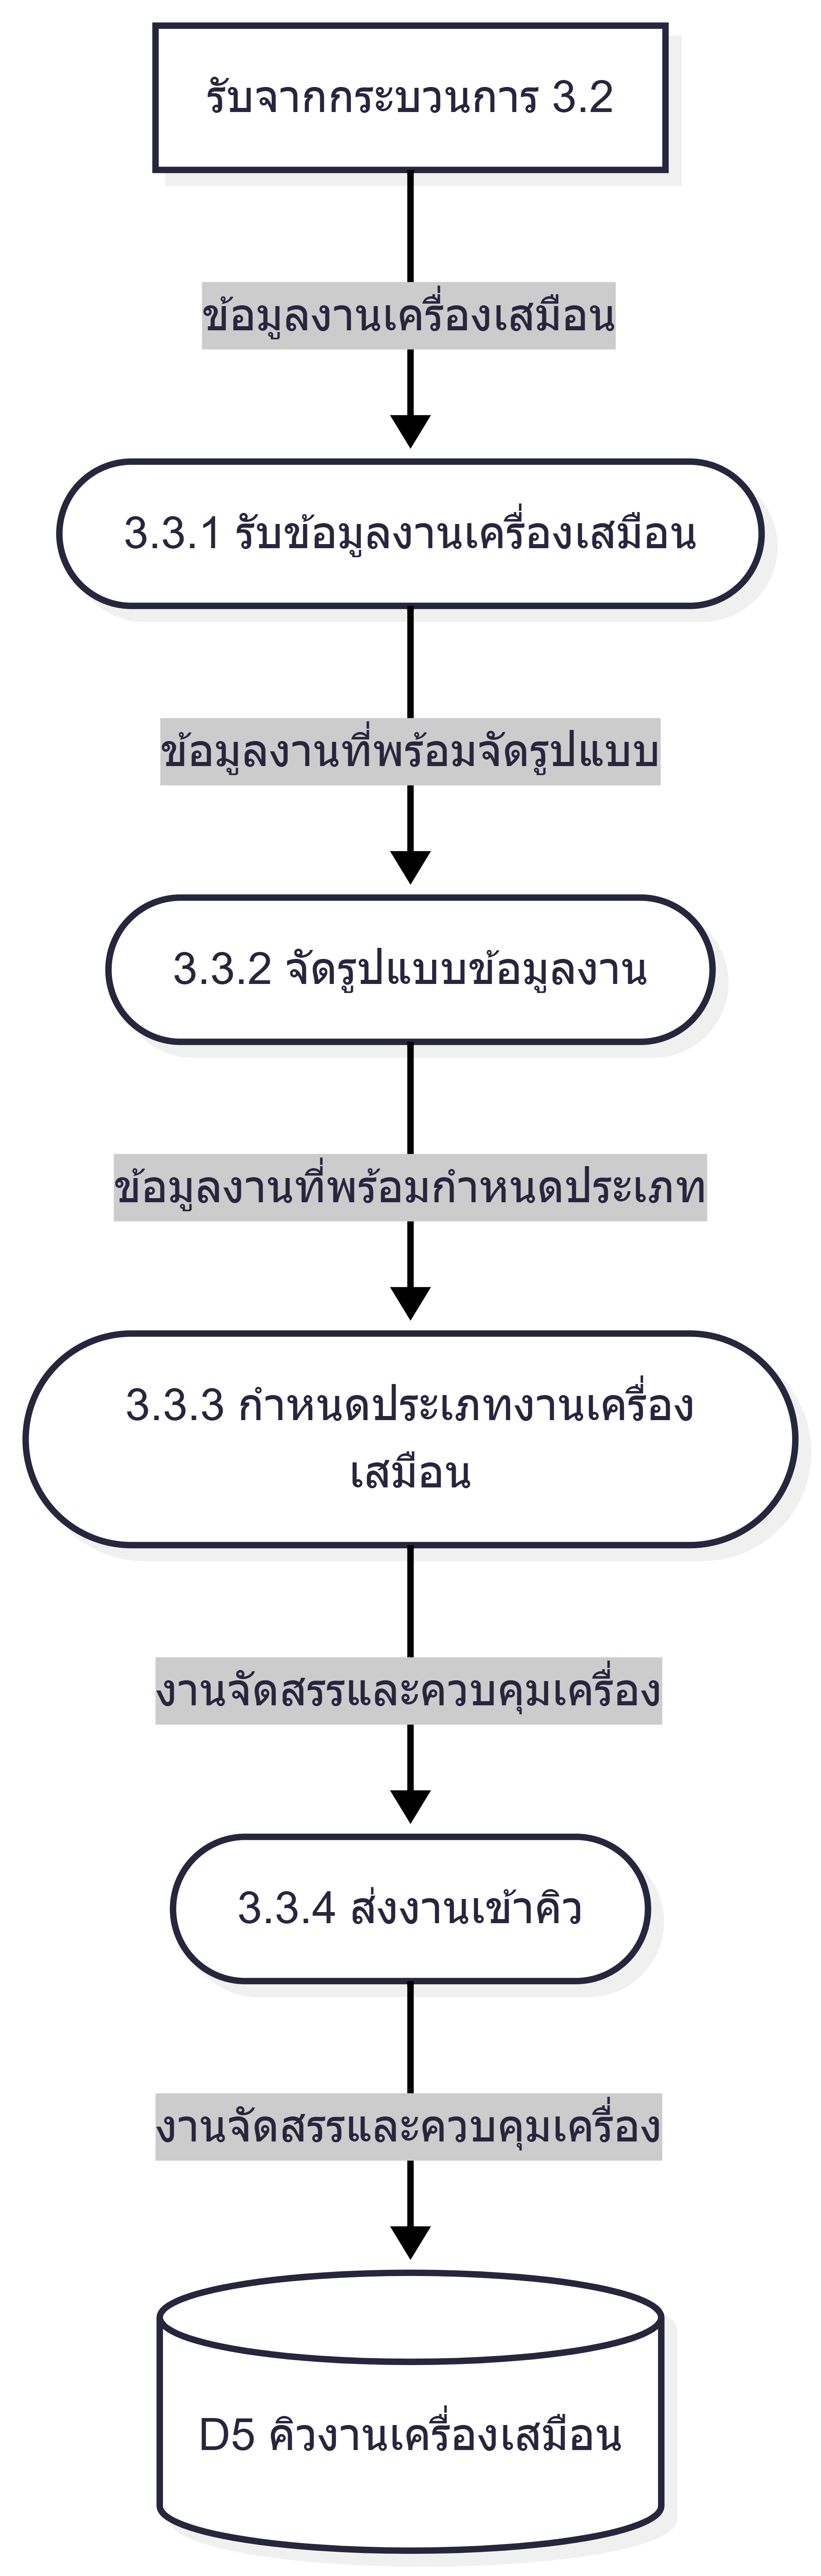
\includegraphics[width=0.35\textwidth]{Image/diagram/chapter3-dataflow-level2-process3-3.png}
    \caption{\fontSixTeen{แผนภาพการไหลของข้อมูลระดับที่ 2 ของกระบวนการ 3.3 การส่งงานเข้าคิว}}
    \label{fig3:data_flow_level_2_queue}
\end{figure}

\hspace*{1.3em} %ย่อหน้า
\textbf{กระบวนการ 3.3 การส่งงานเข้าคิว} (ภาพที่ \ref{fig3:data_flow_level_2_queue}) ระบบจะสร้าง payload ของงานโดยเก็บเฉพาะตัวระบุ (เช่น instanceId, userId, action) และข้อมูลที่จำเป็นขั้นต่ำ เพื่อหลีกเลี่ยงข้อมูลซ้ำซ้อนหรือข้อมูลล้าสมัยในคิว จากนั้นจึงส่งงานเข้าสู่ Redis-backed BullMQ พร้อมกำหนดชนิดงาน (เช่น provision/deprovision/toggle status) และอัปเดตสถานะงานในฐานข้อมูลเพื่อสะท้อนว่าอยู่ระหว่างรอประมวลผล วิธีนี้ช่วยให้การ retry มีความปลอดภัย เพราะ worker สามารถอ่านข้อมูลฉบับล่าสุดจากฐานข้อมูลก่อนลงมือปฏิบัติจริง

\begin{figure}[H]
    \centering
    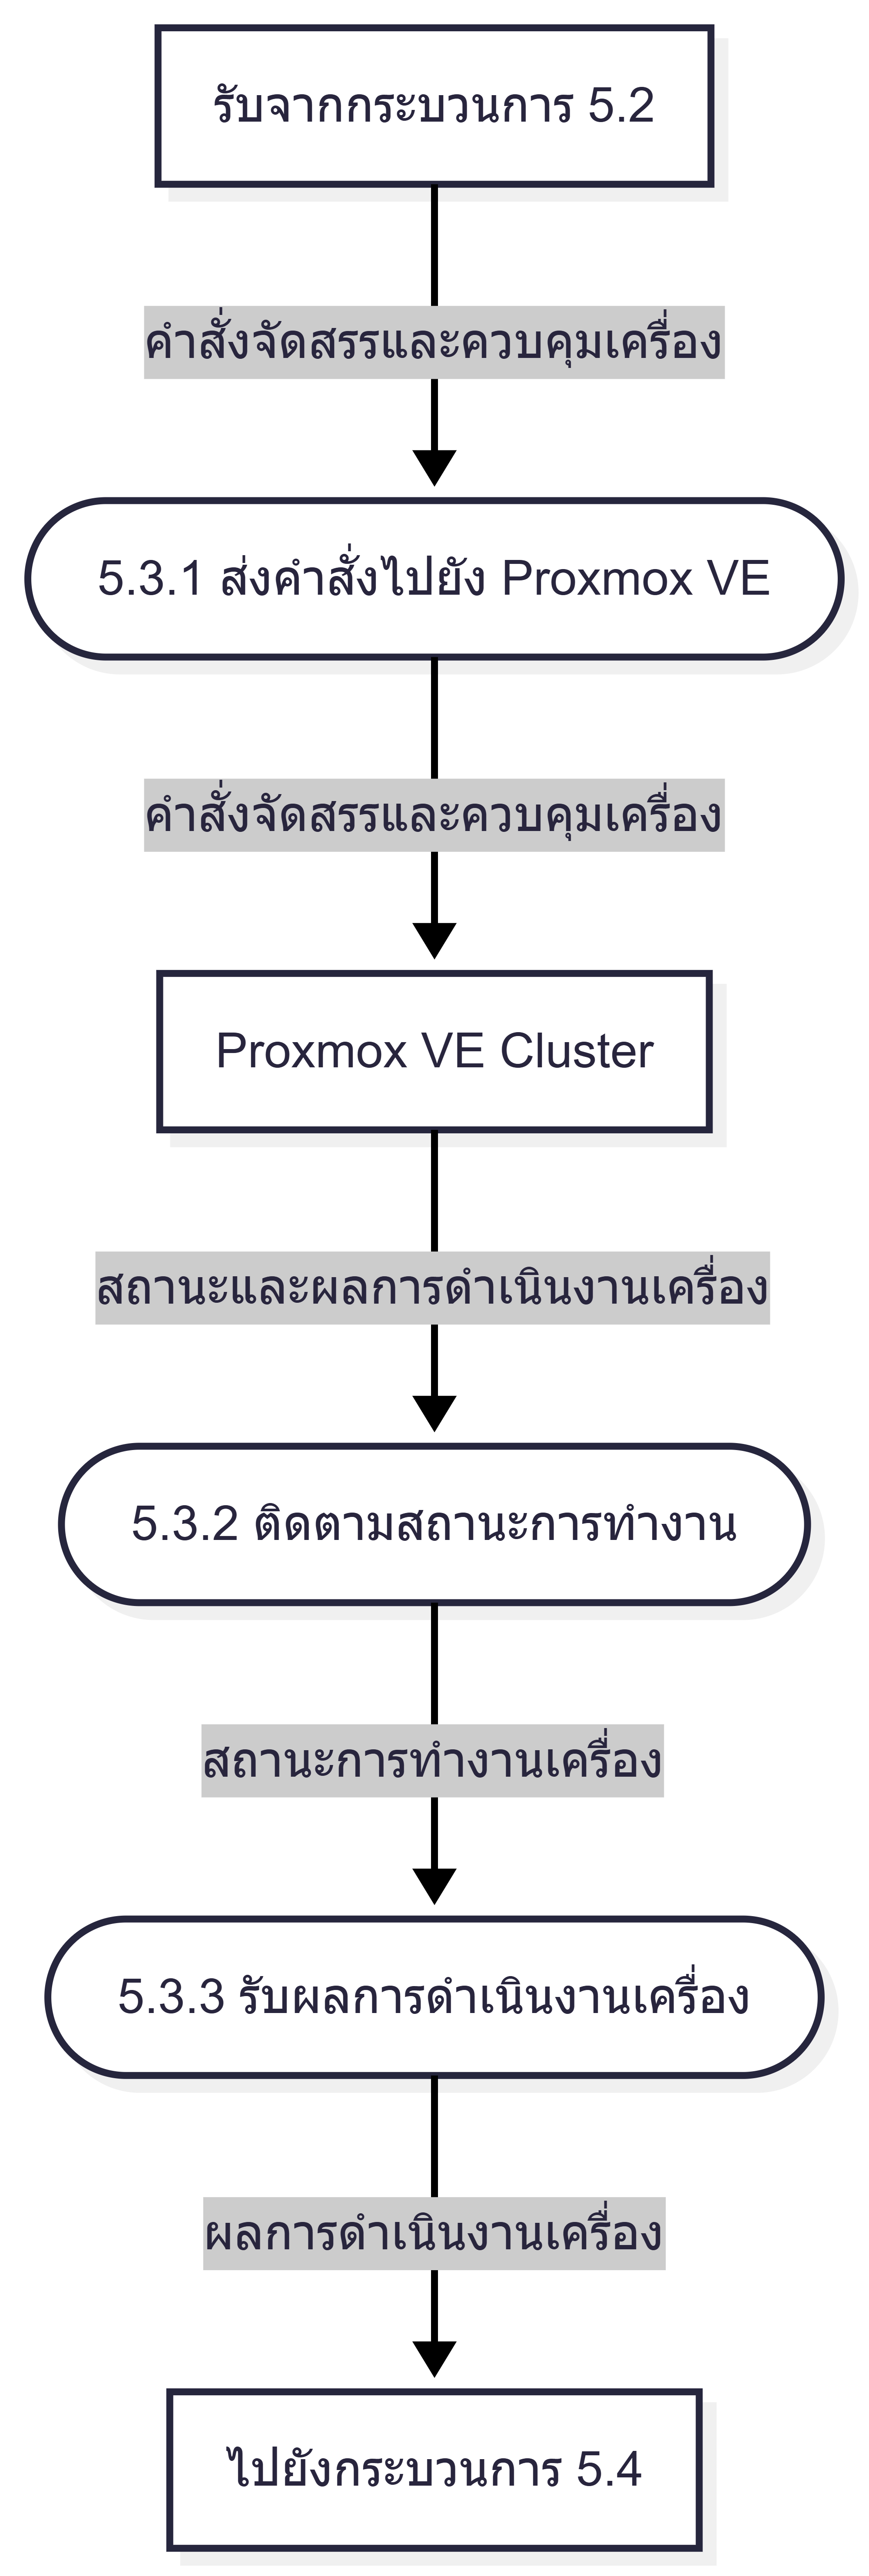
\includegraphics[width=0.35\textwidth]{Image/diagram/chapter3-dataflow-level2-process5-3.png}
    \caption{\fontSixTeen{แผนภาพการไหลของข้อมูลระดับที่ 2 ของกระบวนการ 5.3 การดำเนินการบน Proxmox VE}}
    \label{fig3:data_flow_level_2_pve}
\end{figure}

\hspace*{1.3em} %ย่อหน้า
\textbf{กระบวนการ 5.3 การดำเนินการบน Proxmox VE} (ภาพที่ \ref{fig3:data_flow_level_2_pve}) เริ่มจาก worker (Yuzu) รับงานจากคิวและโหลดรายละเอียด instance จากฐานข้อมูลเพื่อประกอบคำสั่ง จากนั้นเรียก Proxmox VE API เพื่อดำเนินการตามชนิดงาน (สร้าง/ลบ/เริ่ม/หยุด/รีสตาร์ท) พร้อมตรวจสอบผลลัพธ์และบันทึกสถานะงานเป็นช่วง ๆ หากเกิดข้อผิดพลาด worker จะบันทึกเหตุการณ์และสถานะล้มเหลวเพื่อให้ระบบแจ้งกลับผู้ใช้ได้อย่างถูกต้อง และหากเป็นกรณีที่รองรับการ retry จะสามารถหยิบงานขึ้นมาทำซ้ำได้โดยอ้างอิงสถานะล่าสุดในฐานข้อมูลเพื่อหลีกเลี่ยงการสร้าง VM ซ้ำหรือเปลี่ยนสถานะผิดพลาด

\newpage
\subsection{การออกแบบหน้าจอการทำงาน}
\hspace*{1.3em} %ย่อหน้า
การออกแบบหน้าจอการทำงานของระบบแพลตฟอร์มคลัสเตอร์เสมือนได้รับการออกแบบให้มีความสะดวกในการใช้งานและการเข้าถึงข้อมูลที่จำเป็น โดยแบ่งออกเป็นหน้าจอหลัก ๆ ดังนี้
\begin{mycustomitem}
    \item \textbf{หน้าจอเข้าสู่ระบบ (Login Page)} หน้าจอสำหรับผู้ใช้ในการเข้าสู่ระบบผ่านการยืนยันตัวตน
    \item \textbf{หน้าจอแดชบอร์ด (Dashboard)} แสดงภาพรวมสถานะเครื่องเสมือน รายการคำร้องขอ และข้อมูลผู้ใช้
    \item \textbf{หน้าจอจัดการเครื่องเสมือน (Instance Management)} สำหรับผู้ใช้ในการดูรายละเอียดเครื่องเสมือน เช่น สถานะ การเชื่อมต่อ และการจัดการเครื่อง
    \item \textbf{หน้าจอคำร้องขอเครื่องเสมือน (Instance Request)} สำหรับผู้ใช้ในการส่งคำร้องขอการใช้งานเครื่องเสมือน
    \item \textbf{หน้าจอจัดการคำร้องขอ (Request Management)} สำหรับเจ้าหน้าที่ในการตรวจสอบและอนุมัติคำร้องขอเครื่องเสมือน
\end{mycustomitem}
โดยมีการออกแบบหน้าจอหลัก ๆ ดังแสดงในภาพที่ \ref{fig3:login_page} – \ref{fig3:request_management}

\begin{figure}[H]
    \centering
    \fbox{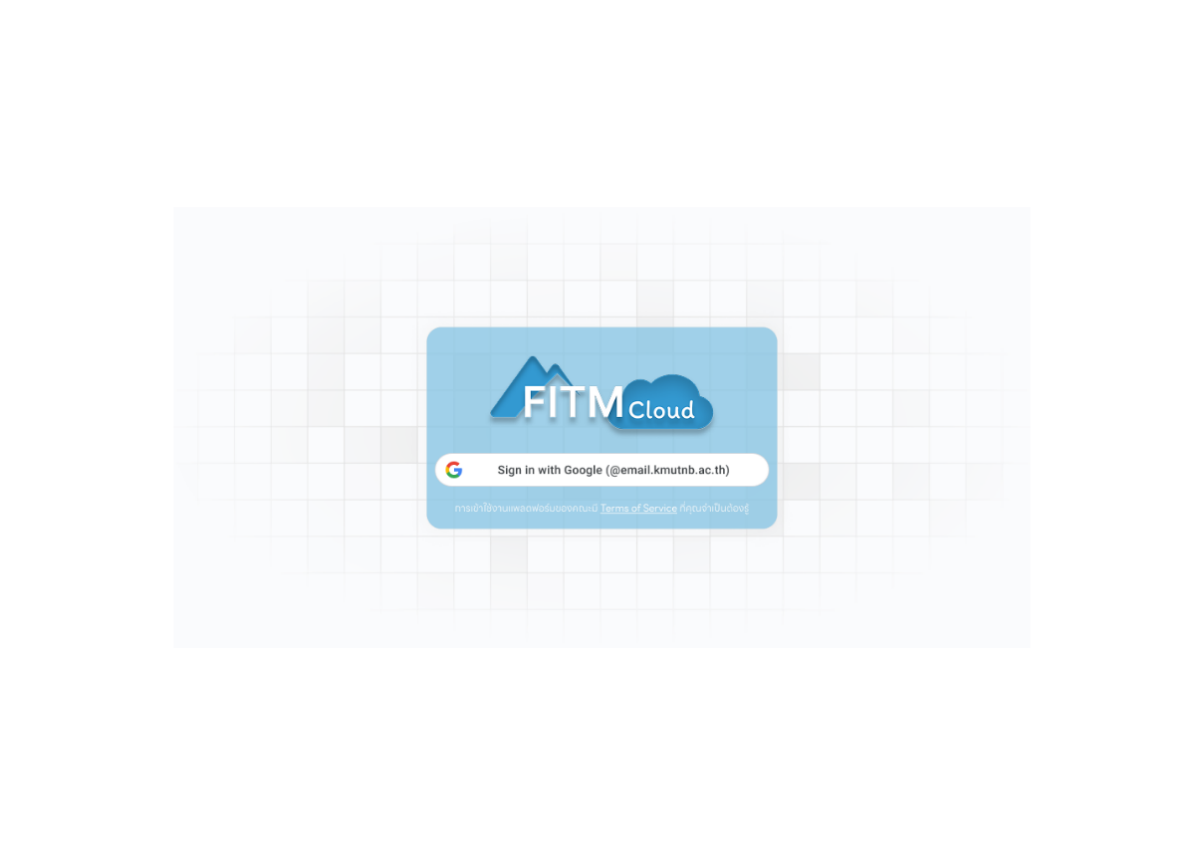
\includegraphics[width=0.9\textwidth]{Image/design/image2.png}}
    \caption{\fontSixTeen{หน้าจอเข้าสู่ระบบ (Login Page)}}
    \label{fig3:login_page}
\end{figure}

\begin{figure}[H]
    \centering
    \fbox{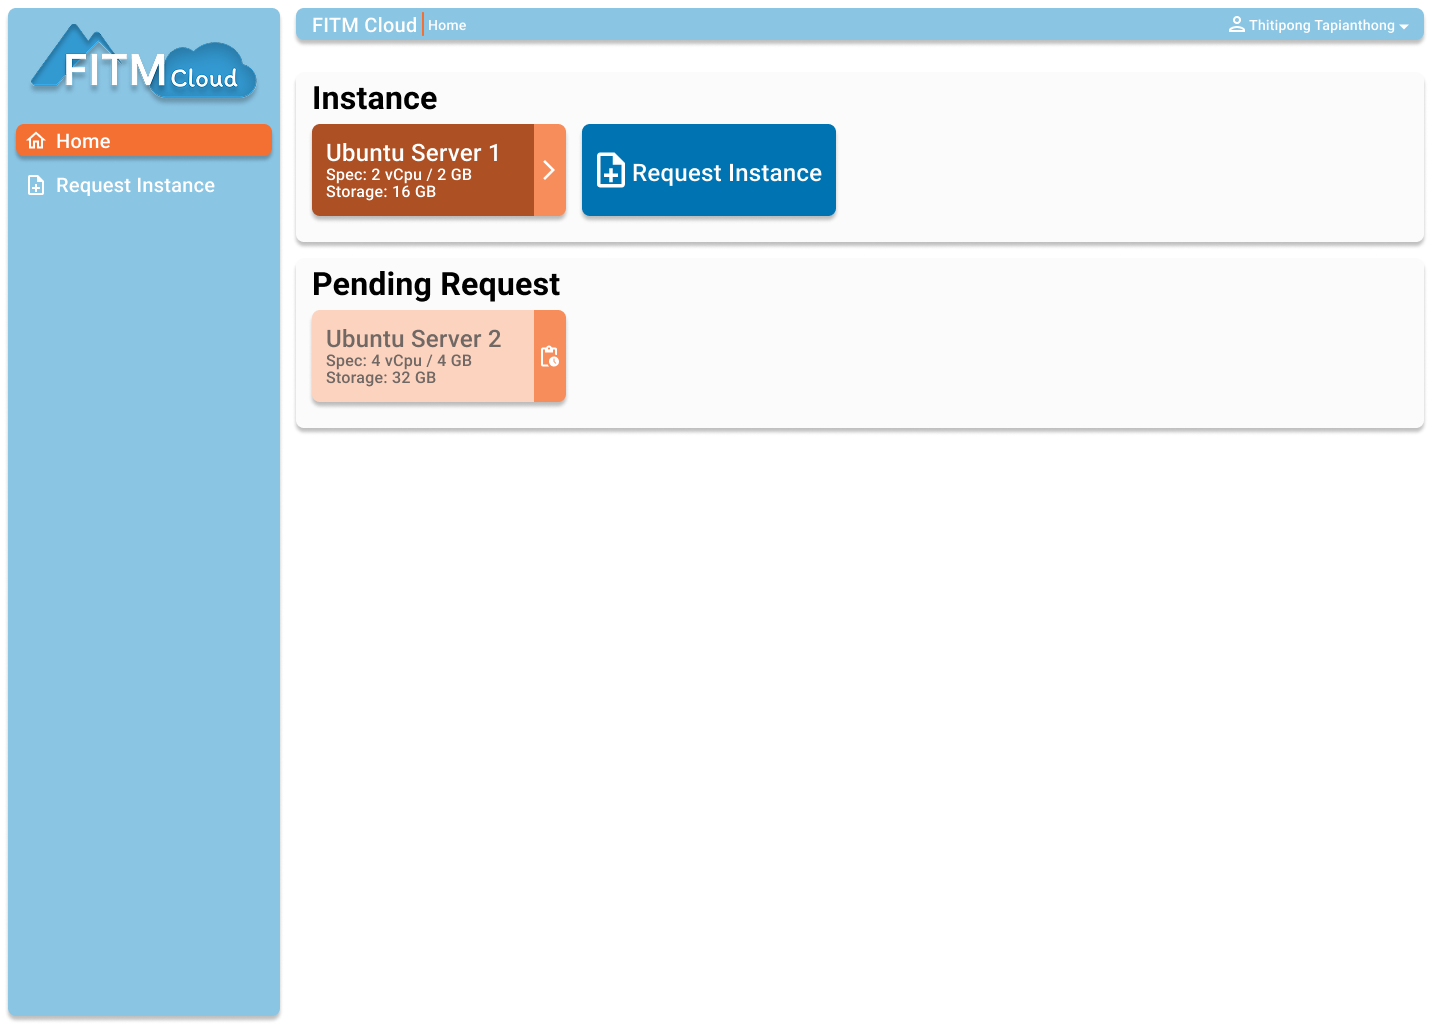
\includegraphics[width=0.9\textwidth]{Image/design/image3.png}}
    \caption{\fontSixTeen{หน้าจอแดชบอร์ด (Dashboard)}}
    \label{fig3:dashboard}
\end{figure}

\begin{figure}[H]
    \centering
    \fbox{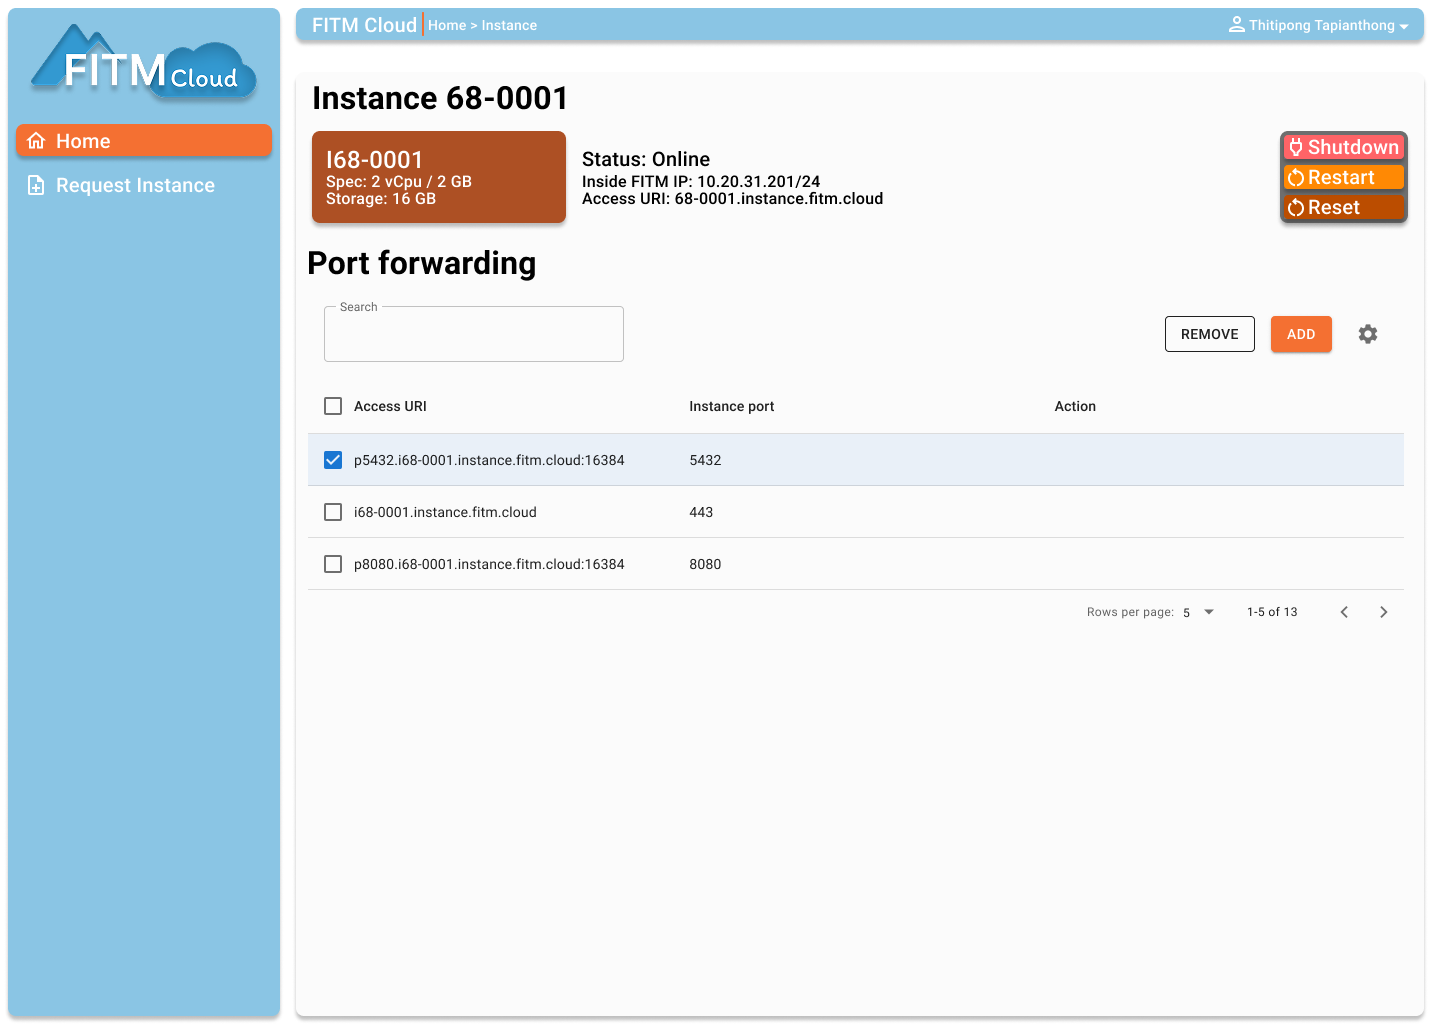
\includegraphics[width=0.9\textwidth]{Image/design/image5.png}}
    \caption{\fontSixTeen{หน้าจอจัดการเครื่องเสมือน (Instance Management)}}
    \label{fig3:instance_management}
\end{figure}

\begin{figure}[H]
    \centering
    \fbox{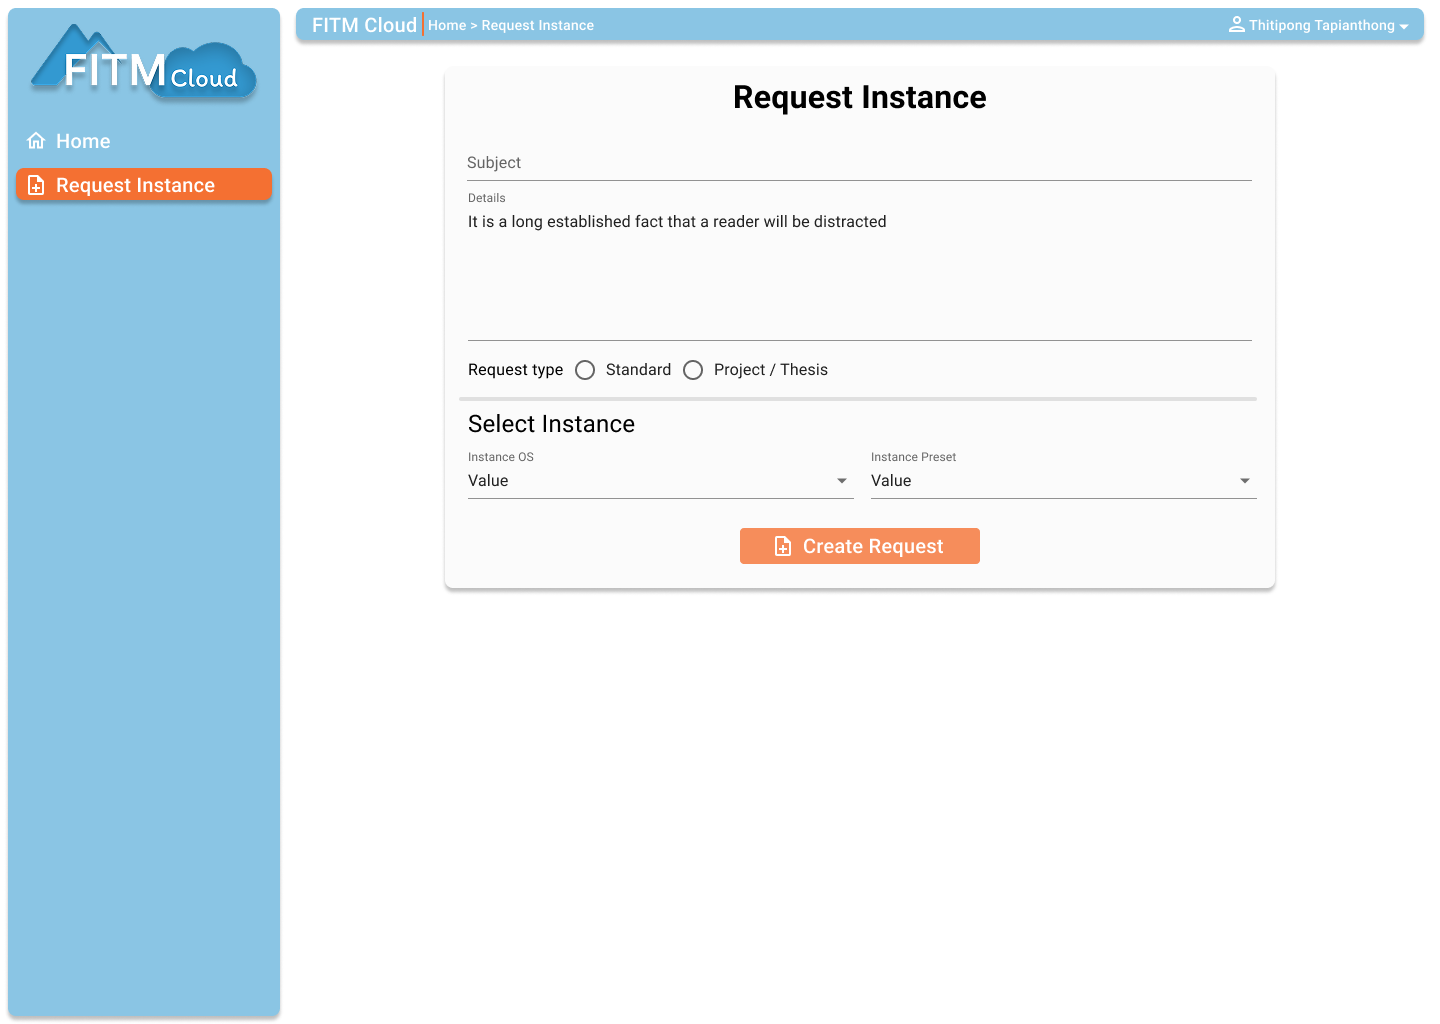
\includegraphics[width=0.9\textwidth]{Image/design/image4.png}}
    \caption{\fontSixTeen{หน้าจอคำร้องขอเครื่องเสมือน (Instance Request)}}
    \label{fig3:instance_request}
\end{figure}

\begin{figure}[H]
    \centering
    \fbox{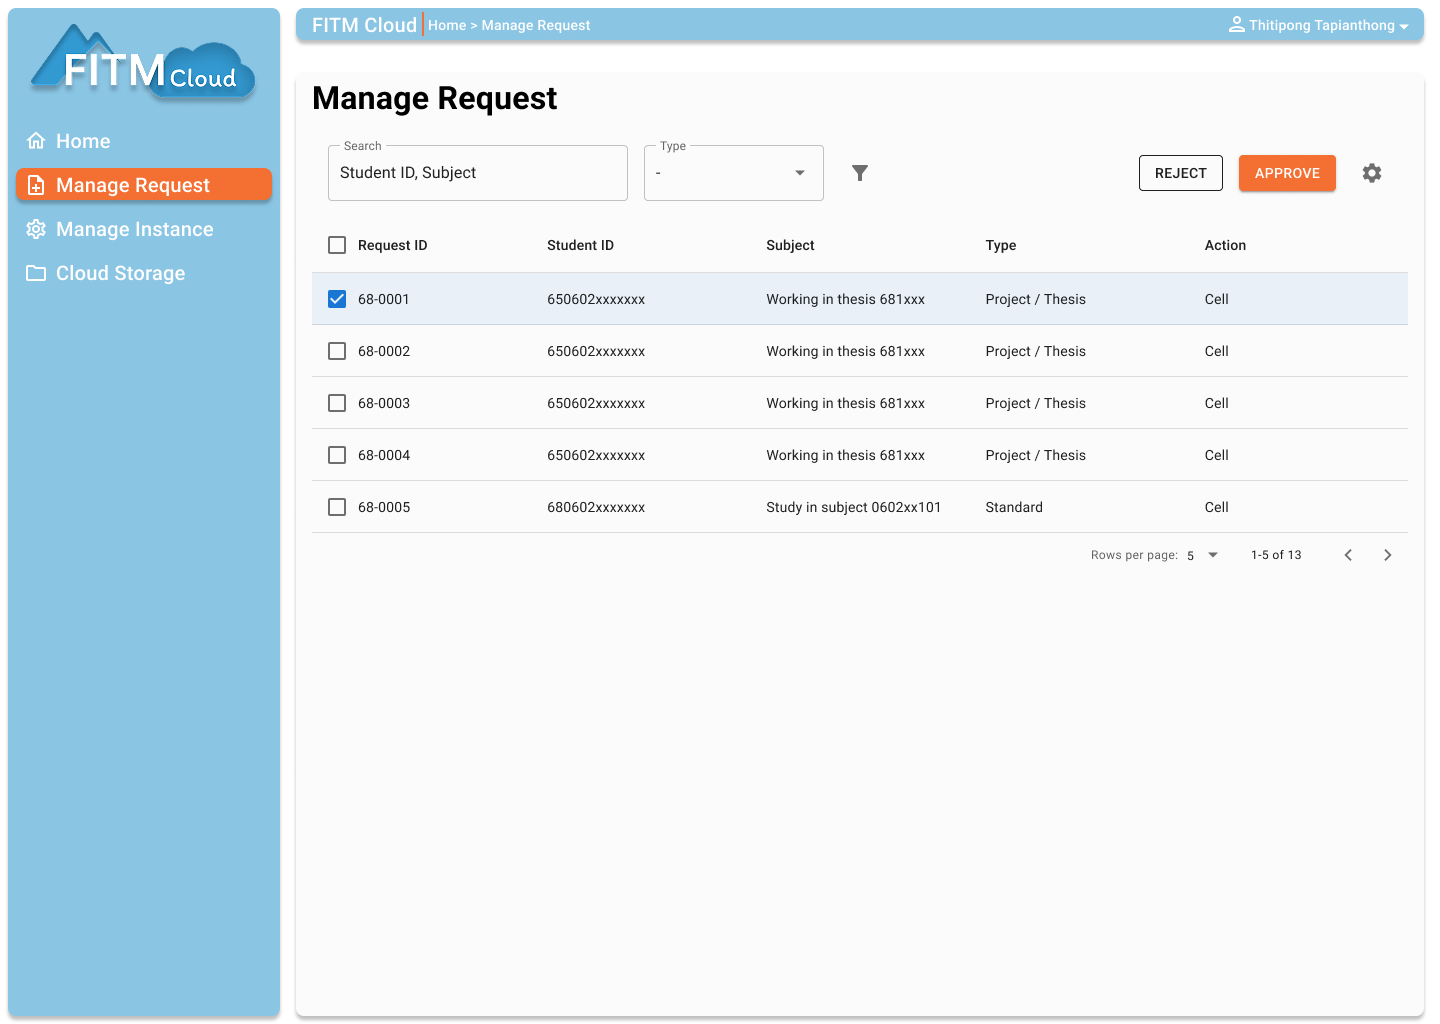
\includegraphics[width=0.9\textwidth]{Image/design/image7.png}}
    \caption{\fontSixTeen{หน้าจอจัดการคำร้องขอ (Request Management)}}
    \label{fig3:request_management}
\end{figure}

\newpage
% 3.3.2
\subsection{การออกแบบฐานข้อมูล}

\hspace*{1.3em} %ย่อหน้า
ระบบใช้ PostgreSQL เป็นฐานข้อมูลหลัก และใช้ Prisma ORM ในการกำหนดสคีมาและสร้างชั้นเข้าถึงข้อมูล โดยในฉบับพัฒนาปัจจุบันโครงสร้างฐานข้อมูลสามารถสรุปเป็นกลุ่มข้อมูลหลักดังนี้
\begin{mycustomitem}
    \item \textbf{Authentication and Role Management} เช่น User, Session, Account, Verification และ PlatformUser สำหรับจัดการตัวตนผู้ใช้งาน เซสชัน และบทบาท ADMIN, INSTRUCTOR, STUDENT
    \item \textbf{Academic Structure} เช่น Course, Semester, CourseOffering และ InstructorSearch สำหรับเชื่อมโยงรายวิชา ภาคการศึกษา และผู้สอน
    \item \textbf{Virtualization Resources} เช่น PVENode, PVENetwork, PVENetworkIP, PVETemplate และ PVEVM สำหรับสะท้อนทรัพยากรที่เกี่ยวข้องกับ Proxmox VE
    \item \textbf{Request Workflow} เช่น Request, ExtendedRequest, RequestAuditLog และ ExtendedRequestAuditLog สำหรับคำร้องขอเครื่องเสมือน การขยายสิทธิ์การใช้งาน และประวัติการอนุมัติ
    \item \textbf{Instance Management} เช่น Instance, InstanceReverseProxy, InstanceAuditLog และ PlatformSSHKey สำหรับข้อมูลเครื่องเสมือน ช่องทางการเชื่อมต่อ และบันทึกการเปลี่ยนแปลง
    \item \textbf{Platform Storage} เช่น PlatformFile สำหรับการจัดเก็บไฟล์
\end{mycustomitem}

% แผนภาพนี้ถูกสร้างจากไฟล์ Mermaid: docs/database/db-overview.mmd
\begin{figure}[H]
    \centering
    
\includegraphics[width=1.0\textwidth]{Image/diagram/database/db-overview.png}
    \caption{\fontSixTeen{แผนภาพโครงสร้างฐานข้อมูลของระบบภาพรวม (ER Diagram Overview)}}
    \label{fig3:database_schema}
\end{figure}

% แผนภาพนี้ถูกสร้างจากไฟล์ Mermaid: docs/database/db-auth.mmd
\begin{figure}[H]
    \centering
    
\includegraphics[width=1.0\textwidth]{Image/diagram/database/db-auth.png}
    \caption{\fontSixTeen{แผนภาพ ER กลุ่มข้อมูลการยืนยันตัวตนและผู้ใช้งาน}}
    \label{fig3:database_schema-1}
\end{figure}

% แผนภาพนี้ถูกสร้างจากไฟล์ Mermaid: docs/database/db-academic.mmd
\begin{figure}[H]
    \centering
    
\includegraphics[width=1.0\textwidth]{Image/diagram/database/db-academic.png}
    \caption{\fontSixTeen{แผนภาพ ER กลุ่มข้อมูลโครงสร้างวิชาการ}}
    \label{fig3:database_schema-2}
\end{figure}

% แผนภาพนี้ถูกสร้างจากไฟล์ Mermaid: docs/database/db-pve.mmd
\begin{figure}[H]
    \centering
    
\includegraphics[width=1.0\textwidth]{Image/diagram/database/db-pve.png}
    \caption{\fontSixTeen{แผนภาพ ER กลุ่มข้อมูลโครงสร้างพื้นฐาน Proxmox VE}}
    \label{fig3:database_schema-3}
\end{figure}

% แผนภาพนี้ถูกสร้างจากไฟล์ Mermaid: docs/database/db-instance.mmd
\begin{figure}[H]
    \centering
    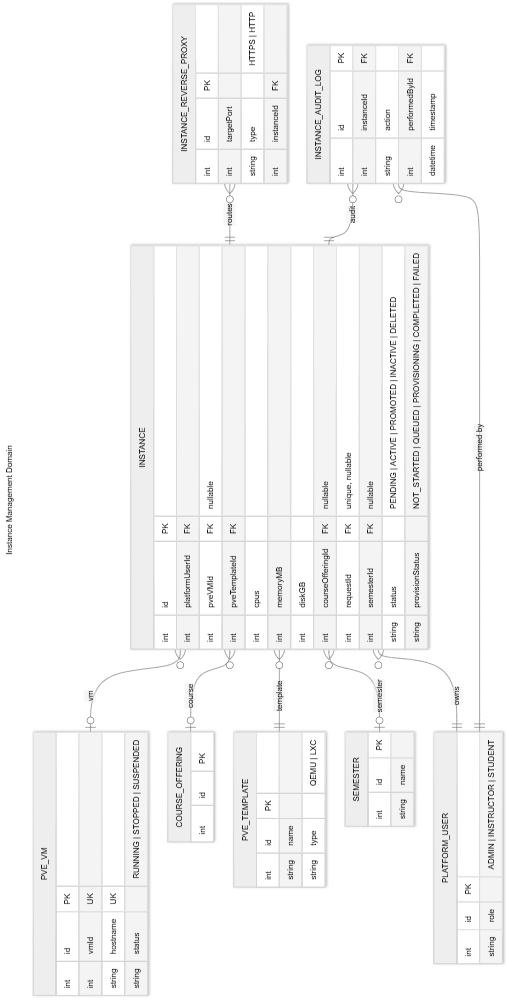
\includegraphics[width=0.75\textwidth]{Image/diagram/database/db-instance_90.png}
    \caption{\fontSixTeen{แผนภาพ ER กลุ่มข้อมูลการจัดการเครื่องเสมือน}}
    \label{fig3:database_schema-4}
\end{figure}

% แผนภาพนี้ถูกสร้างจากไฟล์ Mermaid: docs/database/db-request.mmd
\begin{figure}[H]
    \centering
    
\includegraphics[width=0.9\textwidth]{Image/diagram/database/db-request.png}
    \caption{\fontSixTeen{แผนภาพ ER กลุ่มข้อมูลคำร้องขอและกระบวนการอนุมัติ}}
    \label{fig3:database_schema-5}
\end{figure}

% แผนภาพนี้ถูกสร้างจากไฟล์ Mermaid: docs/database/db-storage.mmd
\begin{figure}[H]
    \centering
    
\includegraphics[width=0.75\textwidth]{Image/diagram/database/db-storage.png}
    \caption{\fontSixTeen{แผนภาพ ER กลุ่มข้อมูลพื้นที่จัดเก็บไฟล์}}
    \label{fig3:database_schema-6}
\end{figure}

\hspace*{1.3em} %ย่อหน้า
จากภาพที่ \ref{fig3:database_schema} – \ref{fig3:database_schema-6} จะเห็นได้ว่าการออกแบบฐานข้อมูลไม่ได้ครอบคลุมเฉพาะข้อมูลผู้ใช้และเครื่องเสมือนเท่านั้น แต่ยังรวมถึงโครงสร้างทางวิชาการ ประวัติการอนุมัติ การจัดการ reverse proxy และระบบจัดเก็บไฟล์ภายในแพลตฟอร์มด้วย ทั้งนี้ได้แบ่งแผนภาพเป็น 6 กลุ่มตามโดเมนข้อมูล ได้แก่ การยืนยันตัวตน โครงสร้างวิชาการ โครงสร้างพื้นฐาน Proxmox VE การจัดการเครื่องเสมือน กระบวนการคำร้องขอ และพื้นที่จัดเก็บไฟล์ การออกแบบในลักษณะนี้ทำให้ Momoi สามารถทำหน้าที่เป็นศูนย์กลางของข้อมูลธุรกรรม ขณะที่ Yuzu ใช้ข้อมูลเดียวกันในการอ้างอิงระหว่างการประมวลผลคำสั่งบน Proxmox VE

\begin{table}[H]
    \caption{\fontSixTeen{สรุปกลุ่มข้อมูลหลักจาก Prisma Schema ฉบับปัจจุบัน}}\label{tab3:db_domain_overview}
    \fontSixTeen
    \renewcommand{\arraystretch}{1.2}
    \begin{tabularx}{\textwidth}{|L|X|}
        \hline
	        \textbf{กลุ่มข้อมูล} & \multicolumn{1}{|>{\centering\arraybackslash}X|}{\textbf{เอนทิตีหลัก}} \\
        \hline
        Authentication และ RBAC & User, Session, Account, Verification, PlatformUser \\
        โครงสร้างวิชาการ & Course, Semester, CourseOffering, InstructorSearch \\
        ทรัพยากร Proxmox VE & PVENode, PVENetwork, PVENetworkIP, PVETemplate, PVEVM \\
        กระบวนการคำร้องขอ & Request, ExtendedRequest, RequestAuditLog, ExtendedRequestAuditLog \\
        การจัดการเครื่องเสมือน & Instance, InstanceReverseProxy, InstanceAuditLog, PlatformSSHKey \\
        พื้นที่จัดเก็บไฟล์ & PlatformFile \\
        \hline
    \end{tabularx}
\end{table}

\begin{table}[H]
    \caption{\fontSixTeen{รายการ Enum สำคัญในสคีมาฐานข้อมูลฉบับปัจจุบัน}}\label{tab3:db_enums_current}
    \fontSixTeen
    \renewcommand{\arraystretch}{1.2}
    \begin{tabularx}{\textwidth}{|l|L|}
        \hline
	        \textbf{ชื่อ Enum} & \multicolumn{1}{|>{\centering\arraybackslash}X|}{\textbf{ค่า}} \\
        \hline
        PlatformRole & ADMIN, INSTRUCTOR, STUDENT \\
        PVEVMStatus & RUNNING, STOPPED, SUSPENDED \\
        PVEVMType & QEMU, LXC \\
        InstanceStatus & PENDING, ACTIVE, PROMOTED, INACTIVE, DELETED \\
        InstanceProvisionStatus & NOT\_STARTED, QUEUED, PROVISIONING, COMPLETED, FAILED \\
        ReverseProxyType & HTTPS, HTTP \\
        ApprovalStatus & PENDING, APPROVED, REJECTED, CANCELLED \\
        \hline
    \end{tabularx}
\end{table}

% 3.3.3
\subsection{การออกแบบ API และการสื่อสาร}

\hspace*{1.3em} %ย่อหน้า
ระบบใช้ RESTful API เป็นหลักในการสื่อสารระหว่างส่วนประกอบ โดยมีการออกแบบดังนี้
\begin{mycustomitem}
    \item \textbf{Authentication Endpoints} ให้บริการผ่านเส้นทาง `/api/auth` โดย Momoi เป็นผู้ดูแลการยืนยันตัวตน Session และ OAuth callback ขณะที่ Midori จะใช้งานเส้นทางดังกล่าวผ่าน better-auth client
    \item \textbf{Platform API Endpoints} ให้บริการโดย Momoi ครอบคลุมโดเมนหลัก เช่น Academic Management, Request Workflow, Instance Management, Reverse Proxy Management และ Storage Management
    \item \textbf{Documentation and Telemetry Endpoints} ใช้สำหรับสร้าง OpenAPI Documentation, Metrics และ Traces เพื่อสนับสนุนการทดสอบและการติดตามสถานะของระบบ โดยกระจายอยู่ตามบทบาทของแต่ละบริการ
\end{mycustomitem}

\hspace*{1.3em} %ย่อหน้า
ตารางที่ \ref{tab3:api_groups} สรุปกลุ่ม API หลักของ Momoi พร้อมระดับการยืนยันตัวตนที่ต้องการ โดย Momoi เปิดเผย API ด้านแพลตฟอร์มเหล่านี้ผ่าน Elysia.js ซึ่งสร้าง OpenAPI Specification โดยอัตโนมัติ ทำให้ Midori สามารถนำข้อมูล Schema ไปสร้างชนิดข้อมูลฝั่ง Client ได้โดยตรงโดยไม่ต้องเขียนซ้ำ

\begin{table}[H]
    \caption{\fontSixTeen{สรุปกลุ่ม API หลักของบริการ Momoi}}\label{tab3:api_groups}
    \fontSixTeen
    \renewcommand{\arraystretch}{1.2}
    \begin{tabularx}{\textwidth}{|l|X|}
        \hline
        \textbf{กลุ่ม API} & \multicolumn{1}{|>{\centering\arraybackslash}X|}{\textbf{คำอธิบาย}} \\
        \hline
        Public & ข้อมูลสาธารณะ เช่น ภาคการศึกษาปัจจุบันและที่กำลังจะมาถึง \\
        Auth & Login, Logout, Session, OAuth callback \\
        Academic & รายวิชา ภาคการศึกษา ผู้สอน และการเปิดสอน \\
        Request & สร้างและจัดการคำร้องขอเครื่องเสมือน ทั้ง Request และ ExtendedRequest \\
        Instance & เครื่องเสมือน Reverse Proxy Audit Log และ SSH Key \\
        Storage & ไฟล์ โฟลเดอร์ การแบ่งปัน และสิทธิ์การเข้าถึง \\
        Admin & จัดการ PVE Node PVE Template PVE Network และ Platform User \\
        \hline
    \end{tabularx}
\end{table}

\hspace*{1.3em} %ย่อหน้า
การยืนยันตัวตนของระบบออกแบบให้ใช้ Session ผ่านชุด endpoint `/api/auth` ซึ่งใช้ `better-auth` และข้อมูลผู้ใช้ในฐานข้อมูลร่วมกัน จากนั้นเมื่อ Midori เรียก API ของ Momoi ต่อไป Momoi จะตรวจสอบ session และดึงข้อมูล PlatformUser จากฐานข้อมูลเพื่อกำหนดบทบาท (ADMIN, INSTRUCTOR, STUDENT) ก่อนอนุมัติคำขอ แนวทางนี้ทำให้การยืนยันตัวตนและการกำหนดสิทธิ์เชื่อมต่อกับ business logic ของแพลตฟอร์มได้โดยตรง และลดความซับซ้อนของ topology ที่ต้องติดตามในเอกสารและการติดตั้งใช้งาน

% 3.3.4
\subsection{การออกแบบระบบ Message Queue}

\hspace*{1.3em} %ย่อหน้า
ระบบรองรับการประมวลผลแบบ Asynchronous โดยใช้ Redis ร่วมกับ BullMQ เป็นกลไก Message Queue ระหว่าง Momoi และ Yuzu คิวหลักในฉบับพัฒนาปัจจุบันประกอบด้วย
\begin{mycustomitem}
    \item \textbf{Provision Queue} สำหรับงานสร้างและจัดสรรเครื่องเสมือนใหม่
    \item \textbf{Deprovision Queue} สำหรับงานลบหรือคืนทรัพยากรของเครื่องเสมือน
    \item \textbf{Toggle Status Queue} สำหรับงานเปลี่ยนสถานะของเครื่อง เช่น Start, Stop และ Restart
\end{mycustomitem}

\hspace*{1.3em} %ย่อหน้า
ในระดับการติดตั้งใช้งานจริง คิวเหล่านี้จะถูกตั้งชื่อแบบผูกกับ environment นำหน้าชื่อคิวเพื่อแยกงานของแต่ละสภาพแวดล้อมออกจากกันอย่างชัดเจน

\hspace*{1.3em} %ย่อหน้า
ข้อมูลที่ถูกส่งเข้าแต่ละงานจะเก็บเฉพาะตัวระบุที่จำเป็น เช่น `instanceId`, `userId` และ action ที่ต้องการเปลี่ยนแปลง จากนั้น Yuzu จะอ่านข้อมูลฉบับเต็มจากฐานข้อมูลก่อนดำเนินการบน Proxmox VE วิธีการนี้ช่วยลดความซ้ำซ้อนของข้อมูลในคิว ลดโอกาสใช้ข้อมูลที่ล้าสมัย และทำให้การ retry งานมีความปลอดภัยมากขึ้น

\hspace*{1.3em} %ย่อหน้า
ระบบกำหนดนโยบายการทำซ้ำงาน (retry policy) เพื่อรองรับความล้มเหลวชั่วคราว เช่น การเชื่อมต่อ Proxmox VE ขัดข้อง หรือ VM อยู่ระหว่างเปลี่ยนสถานะ โดยงานที่ล้มเหลวจะถูก retry ตามจำนวนครั้งที่กำหนด พร้อมการหน่วงเวลาแบบ exponential backoff ระหว่างครั้ง หากยังล้มเหลวเกินจำนวนที่กำหนดจะถูกย้ายเข้า failed job queue เพื่อให้ผู้ดูแลระบบตรวจสอบในภายหลัง ตารางที่ \ref{tab3:queue_jobs} สรุปคิวงานหลักพร้อมข้อมูลที่ส่งพร้อมแต่ละงานและผลลัพธ์ที่คาดหวัง

\begin{table}[H]
    \caption{\fontSixTeen{สรุปคิวงานหลักและโครงสร้างข้อมูลงาน}}\label{tab3:queue_jobs}
    \fontSixTeen
    \renewcommand{\arraystretch}{1.2}
    \begin{tabularx}{\textwidth}{|l|X|X|}
        \hline
        \textbf{ชื่อคิว} & \multicolumn{1}{|>{\centering\arraybackslash}X|}{\textbf{ข้อมูลหลักในงาน}} & \multicolumn{1}{|>{\centering\arraybackslash}X|}{\textbf{ผลลัพธ์ที่คาดหวัง}} \\
        \hline
        Provision & instanceId, userId & VM ถูกสร้างและพร้อมใช้งาน สถานะ Instance อัปเดตเป็น ACTIVE \\
        Deprovision & instanceId, userId & VM ถูกลบออกจากระบบ สถานะ Instance อัปเดตเป็น DELETED \\
        Toggle Status & instanceId, userId, action (START STOP RESTART) & สถานะ VM และ Instance ถูกอัปเดตให้สอดคล้องกับการสั่ง Start Stop หรือ Restart \\
        \hline
    \end{tabularx}
\end{table}

% Tools and Technologies Used
\section{เครื่องมือและเทคโนโลยีที่ใช้ในการพัฒนา}

% 3.4.1
\subsection{เทคโนโลยี Frontend}

\hspace*{1.3em} %ย่อหน้า
\textbf{Next.js 16 และ React 19} เป็นเทคโนโลยีหลักของส่วน Frontend เนื่องจากมีคุณสมบัติที่เหมาะสมกับการพัฒนาเว็บแอปพลิเคชันเชิงระบบดังนี้
\begin{mycustomitem}
    \item \textbf{App Router} สำหรับการจัดการ Routing แบบใหม่
    \item \textbf{Built-in TypeScript Support} รองรับ Type Safety
    \item \textbf{Integration with API Proxy and OpenAPI Types} ช่วยให้ส่วน Frontend สามารถเชื่อมต่อกับ Momoi ได้อย่างมีชนิดข้อมูลที่ชัดเจนและลดความซ้ำซ้อนของ schema ระหว่าง frontend กับ backend
\end{mycustomitem}

\hspace*{1.3em} %ย่อหน้า
\textbf{Tailwind CSS และชุดคอมโพเนนต์บน Radix UI} ใช้สำหรับการจัดการส่วนติดต่อผู้ใช้ เนื่องจาก
\begin{mycustomitem}
    \item \textbf{Utility-first} เขียน CSS ได้เร็วและมีประสิทธิภาพ
    \item \textbf{Responsive Design} รองรับการแสดงผลบนอุปกรณ์ต่าง ๆ
    \item \textbf{Composable UI Primitives} ช่วยให้สร้างฟอร์ม แดชบอร์ด และกล่องโต้ตอบที่ปรับใช้ซ้ำได้ง่าย
\end{mycustomitem}

% 3.4.2
\subsection{เทคโนโลยี Backend}

\hspace*{1.3em} %ย่อหน้า
\textbf{Elysia.js} เป็น Web Framework ที่ใช้กับ Bun Runtime โดยมีเหตุผลในการเลือกใช้ดังนี้
\begin{mycustomitem}
    \item \textbf{High Performance} มีประสิทธิภาพสูงกว่า Node.js Framework ทั่วไป
    \item \textbf{Type Safety} รองรับ TypeScript แบบเต็มรูปแบบ
    \item \textbf{OpenAPI Integration} สร้าง API Documentation อัตโนมัติ
    \item \textbf{Observability Integration} รองรับการเชื่อมต่อกับ OpenTelemetry และการเก็บข้อมูลด้านประสิทธิภาพของบริการ
\end{mycustomitem}

\hspace*{1.3em} %ย่อหน้า
\textbf{Prisma ORM} ใช้สำหรับการจัดการฐานข้อมูล เนื่องจาก
\begin{mycustomitem}
    \item \textbf{Type-safe Database Client} ป้องกันข้อผิดพลาดในการเขียน Query
    \item \textbf{Database Migrations} จัดการการเปลี่ยนแปลง Schema อย่างเป็นระบบ
    \item \textbf{Centralized Domain Model} ช่วยให้สคีมาของข้อมูลด้านผู้ใช้ คำร้อง เครื่องเสมือน และพื้นที่จัดเก็บอยู่ในรูปแบบเดียวกัน
\end{mycustomitem}

% 3.4.3
\subsection{Infrastructure และ DevOps}

\hspace*{1.3em} %ย่อหน้า
\textbf{Docker} ใช้สำหรับการ Containerization ของแอปพลิเคชันและบริการสนับสนุน เพื่อ
\begin{mycustomitem}
    \item \textbf{Environment Consistency} สภาพแวดล้อมการพัฒนาและ Production เหมือนกัน
    \item \textbf{Easy Deployment} ง่ายต่อการ Deploy และ Scale
    \item \textbf{Resource Isolation} แยกทรัพยากรระหว่างแอปพลิเคชัน
\end{mycustomitem}

\hspace*{1.3em} %ย่อหน้า
\textbf{Docker Compose และ Kubernetes Manifests} ใช้สำหรับการจัดการ Multi-container Application และสภาพแวดล้อมการติดตั้งจริง
\begin{mycustomitem}
    \item \textbf{Service Orchestration} จัดการการเริ่มต้นและหยุดทำงานของ Service
    \item \textbf{Network Management} จัดการเครือข่ายระหว่าง Container
    \item \textbf{Volume Management} จัดการการแชร์ข้อมูลระหว่าง Container
    \item \textbf{Platform Deployment} กำหนดการติดตั้งบริการหลัก เช่น PostgreSQL, Redis, RustFS และชุดระบบสังเกตการณ์การทำงาน
\end{mycustomitem}

\hspace*{1.3em} %ย่อหน้า
\textbf{Observability Stack} ถูกนำมาใช้เพื่อวัดผลและติดตามสภาวะของระบบอย่างต่อเนื่อง
\begin{mycustomitem}
    \item \textbf{Prometheus} สำหรับเก็บ Metrics จากแต่ละบริการ
    \item \textbf{Grafana} สำหรับแสดง Dashboard และภาพรวมของระบบ
    \item \textbf{Loki และ Jaeger} สำหรับเก็บ Logs และ Traces
    \item \textbf{InfluxDB และ Exporters} สำหรับรองรับข้อมูลเชิงสังเกตการณ์เพิ่มเติมในระดับโครงสร้างพื้นฐาน
\end{mycustomitem}

% 3.4.4
\subsection{เครื่องมือการพัฒนา}

\hspace*{1.3em} %ย่อหน้า
\textbf{Version Control และ Collaboration}
\begin{mycustomitem}
    \item \textbf{Git} สำหรับการควบคุมเวอร์ชันของโค้ด
    \item \textbf{GitHub} สำหรับการเก็บโค้ดและการทำงานร่วมกัน
    \item \textbf{GitHub Actions} สำหรับ CI/CD Pipeline
\end{mycustomitem}

\hspace*{1.3em} %ย่อหน้า
\textbf{Code Quality และ Testing}
\begin{mycustomitem}
    \item \textbf{TypeScript-first Development} สำหรับ Static Type Checking ตลอดทุกบริการ
    \item \textbf{OpenAPI Code Generation} สำหรับสร้างชนิดข้อมูลและลดความคลาดเคลื่อนระหว่าง Frontend กับ Backend
    \item \textbf{Repository-specific Linting and Formatting} ใช้เครื่องมือที่เหมาะสมกับแต่ละบริการเพื่อควบคุมคุณภาพของโค้ดก่อนนำขึ้นใช้งาน
\end{mycustomitem}

    %*************************************
% บทที่ 4
%*************************************
\chapterTitle{4}{ผลการดำเนินงาน}

\hspace*{1.3em}
ในการพัฒนาระบบแพลตฟอร์มคลาวด์เพื่อสนับสนุนกิจกรรมการเรียนการสอนและงานวิชาการ ได้ดำเนินการออกแบบและพัฒนาระบบที่ประกอบด้วย 3 บริการซอฟต์แวร์หลัก คือ ส่วนติดต่อผู้ใช้ (Frontend) ส่วนบริการ API (API Service) และส่วนประมวลผลงานจัดการเครื่องเสมือน (VM Operations Service) ร่วมกับบริการสนับสนุนสำหรับการยืนยันตัวตน ฐานข้อมูล ระบบคิวงาน พื้นที่จัดเก็บไฟล์ และระบบติดตามการทำงาน
ในบทนี้จึงนำเสนอผลการดำเนินงานในมุมของโครงสร้างรีโพซิทอรี องค์ประกอบของแต่ละบริการ เทคโนโลยีที่ใช้ เอกสารประกอบการใช้งาน และตัวอย่างหน้าจอของระบบที่พัฒนาขึ้นจริง โดยยึดตามสภาพแวดล้อมของโค้ดปัจจุบันซึ่งแยกเป็นหลายรีโพซิทอรีและติดตั้งใช้งานร่วมกันในลักษณะ Microservices Architecture
\section{โครงสร้างโครงงานหลัก}
\hspace*{1.3em}
จากการออกแบบและพัฒนาระบบแพลตฟอร์มคลาวด์เพื่อสนับสนุนกิจกรรมการเรียนการสอนและงานวิชาการ โครงงานฉบับปัจจุบันไม่ได้จัดเก็บแบบ Monorepo แต่แบ่งออกเป็น 4 รีโพซิทอรีหลักที่ทำงานร่วมกัน ได้แก่ \textbf{Midori}, \textbf{Momoi}, \textbf{Yuzu} และ \textbf{Yuuka} เพื่อให้สามารถพัฒนา ทดสอบ และติดตั้งใช้งานแต่ละส่วนได้อย่างเป็นอิสระ

\subsection{รีโพซิทอรี Midori}
\hspace*{1.3em}
รีโพซิทอรี \textbf{Midori} เป็นส่วนติดต่อผู้ใช้ของระบบ พัฒนาด้วย Next.js และ React ทำหน้าที่นำเสนอหน้าเว็บสำหรับนักศึกษา อาจารย์ และผู้ดูแลระบบ ภายในรีโพซิทอรีนี้มีโครงสร้างสำคัญ เช่นโฟลเดอร์ src/app สำหรับหน้าและ route หลักของระบบ, src/components สำหรับองค์ประกอบส่วนติดต่อผู้ใช้, src/hooks และ src/lib สำหรับตรรกะร่วม, รวมถึงไฟล์กำหนดค่าอย่าง package.json, next.config.ts และ components.json
\begin{mycustomenum2}
    \item \textbf{Landing Page และ Login Flow} สำหรับการเข้าถึงระบบและเข้าสู่กระบวนการยืนยันตัวตน
    \item \textbf{Dashboard ตามบทบาทผู้ใช้} สำหรับนักศึกษา อาจารย์ และผู้ดูแลระบบ
    \item \textbf{Client สำหรับเรียก API} ที่เชื่อมต่อกับ Momoi และบริการยืนยันตัวตนผ่าน OpenAPI
\end{mycustomenum2}
\hspace*{1.3em}
การแยกส่วนติดต่อผู้ใช้ออกมาเป็นรีโพซิทอรีเฉพาะช่วยให้สามารถพัฒนา UI, จัดการ state และทดสอบประสบการณ์ผู้ใช้ได้โดยไม่กระทบกับตรรกะของบริการฝั่ง backend

\subsection{รีโพซิทอรี Momoi}
\hspace*{1.3em}
รีโพซิทอรี \textbf{Momoi} เป็นบริการ API หลักของแพลตฟอร์ม พัฒนาด้วย Bun, Elysia.js และ Prisma ทำหน้าที่เป็นศูนย์กลางของข้อมูลธุรกรรมและตรรกะทางธุรกิจ ภายในประกอบด้วยโฟลเดอร์สำคัญ เช่น src/routes สำหรับกำหนด API, src/service สำหรับ business logic, src/database/prisma สำหรับ schema ของฐานข้อมูล, src/queue สำหรับตัวส่งงานเข้าคิว และ test สำหรับชุดทดสอบ
\begin{mycustomenum2}
    \item \textbf{Academic Management API} สำหรับข้อมูลรายวิชา ภาคการศึกษา ผู้สอน และโครงสร้างที่เกี่ยวข้อง
    \item \textbf{Request และ Instance API} สำหรับจัดการคำร้อง เครื่องเสมือน reverse proxy และประวัติการใช้งาน
    \item \textbf{Storage และ Observability} สำหรับจัดการไฟล์ การเชื่อมต่อ S3-compatible storage และการเปิดเผย OpenAPI, metrics, tracing
\end{mycustomenum2}
\hspace*{1.3em}
รีโพซิทอรีนี้ยังเป็นจุดเชื่อมต่อกับ PostgreSQL, Redis และบริการจัดเก็บไฟล์ ทำให้ Momoi ทำหน้าที่เป็นแกนกลางของแพลตฟอร์มในเชิงข้อมูลและการประสานงานระหว่างบริการ

\subsection{รีโพซิทอรี Yuzu}
\hspace*{1.3em}
รีโพซิทอรี \textbf{Yuzu} เป็นบริการประมวลผลงานเบื้องหลังสำหรับการจัดสรร ลบ และเปลี่ยนสถานะเครื่องเสมือน โดยรับงานจากคิวและเชื่อมต่อกับ Proxmox VE แบบ asynchronous ภายในมีโฟลเดอร์ src/queue สำหรับ worker แต่ละประเภท, src/pve สำหรับ client และชนิดข้อมูลของ Proxmox API, และ src/database สำหรับการอ่านข้อมูลร่วมจาก PostgreSQL

\begin{mycustomenum2}
    \item \textbf{Provision Worker} สำหรับสร้างและเตรียมเครื่องเสมือนใหม่
    \item \textbf{Deprovision Worker} สำหรับคืนทรัพยากรและลบเครื่องที่ไม่ใช้งานแล้ว
    \item \textbf{Toggle Status Worker} สำหรับสั่งเริ่ม หยุด หรือรีสตาร์ตเครื่องเสมือน
\end{mycustomenum2}

\hspace*{1.3em}
การแยก Yuzu ออกมาเป็น worker service ช่วยให้สามารถจัดการงานที่ใช้เวลานานและงานที่ต้อง retry ได้อย่างเหมาะสม โดยไม่ทำให้ API หลักต้องรอผลการทำงานจาก Proxmox VE โดยตรง

\subsection{รีโพซิทอรี Yuuka}
\hspace*{1.3em}
รีโพซิทอรี \textbf{Yuuka} ใช้สำหรับเก็บไฟล์กำหนดค่าการติดตั้งระบบและบริการสนับสนุน เช่น manifest สำหรับ Kubernetes, ตัวอย่าง environment file, เอกสาร observability และไฟล์ docker-compose.yaml สำหรับสภาพแวดล้อมพัฒนา ภายในรีโพซิทอรีนี้มีบริการสำคัญ เช่น PostgreSQL, Redis, RustFS, Prometheus, Grafana, Loki, Jaeger, InfluxDB รวมถึงไฟล์ deployment ของ midori, momoi และ yuzu

\hspace*{1.3em}
โครงสร้างลักษณะนี้ช่วยให้การจัดการโครงสร้างพื้นฐานแยกออกจากโค้ดแอปพลิเคชันอย่างชัดเจน และทำให้สามารถปรับใช้ระบบได้ทั้งในระดับ local development และ cluster environment โดยในภาพรวม Yuuka เป็นจุดที่กำหนด ingress routing และการเชื่อมต่อระหว่างบริการ เช่น การนำคำขอจากผู้ใช้ไปยัง Midori และ Momoi รวมถึงการผูกบริการสนับสนุนเข้ากับระบบหลักอย่างเป็นระบบ

\section{โครงสร้างแอปพลิเคชันและบริการ}
\subsection{ส่วนประกอบหลักของระบบ}
\hspace*{1.3em}
นอกจากการแยกรีโพซิทอรีตามหน้าที่แล้ว แต่ละบริการยังมีไฟล์กำหนดค่าหลักของตนเองเพื่อควบคุมการพัฒนาและการติดตั้งใช้งาน เช่น package.json สำหรับจัดการ dependency และ script, tsconfig.json สำหรับกำหนดค่า TypeScript, Dockerfile สำหรับการสร้าง container image และ README.md สำหรับอธิบายวิธีใช้งานและขั้นตอนการติดตั้ง

\hspace*{1.3em}
ในส่วนของ Momoi และ Yuzu ยังมีไฟล์ prisma.config.ts สำหรับกำหนดค่า Prisma และการเชื่อมต่อฐานข้อมูล ขณะที่ Midori มีไฟล์ next.config.ts, components.json และ postcss.config.mjs เพื่อควบคุมการทำงานของเฟรมเวิร์กและระบบออกแบบส่วนติดต่อผู้ใช้ ส่วน Yuuka ใช้ไฟล์ .yaml จำนวนมากเพื่ออธิบาย topology ของบริการที่ติดตั้งจริง

\subsection{โครงสร้างระบบทั้งหมด}
\hspace*{1.3em}
โดยในสภาพแวดล้อมจริงของการพัฒนาปัจจุบัน โครงสร้างถูกแยกเป็นหลายรีโพซิทอรีตามความรับผิดชอบของบริการ และแต่ละรีโพซิทอรีมีเอกสาร ไฟล์กำหนดค่า และ source code ของตนเองอย่างชัดเจน

\hspace*{1.3em}
นอกจากนี้ยังประกอบด้วยไฟล์สำคัญอีกหลายไฟล์ ได้แก่
\begin{mycustomitem}
    \item Dockerfile ของแต่ละบริการ สำหรับสร้าง container image แยกตามหน้าที่
    \item package.json และ bun.lock หรือไฟล์ lock ที่ใช้ควบคุม dependency
    \item tsconfig.json, prisma.config.ts และไฟล์กำหนดค่าเฉพาะเฟรมเวิร์ก เช่น next.config.ts
    \item ไฟล์ตัวอย่างสภาพแวดล้อม เช่น .env.example และไฟล์ในโฟลเดอร์ yuuka/docs/env
    \item ไฟล์ deployment และ observability
    \item ไฟล์เอกสาร เช่น README.md, docs/API.md, docs/QUEUE.md และเอกสารประกอบในรีโพซิทอรีต่าง ๆ
\end{mycustomitem}
\hspace*{1.3em}
การแบ่งโครงสร้างเป็นหลายรีโพซิทอรีช่วยลด coupling ระหว่างบริการ ทำให้สามารถวางวงจรการพัฒนา ทดสอบ และติดตั้งใช้งานของแต่ละส่วนได้อย่างยืดหยุ่น เมื่อต้องการปรับปรุง frontend, API, worker หรือ infrastructure ก็สามารถทำได้เฉพาะส่วนโดยไม่ต้องแบกรับความซับซ้อนของโครงสร้างแบบรวมศูนย์ขนาดใหญ่

% \begin{figure}[htbp]
% \centering
% \adjustbox{frame, width=0.8\textwidth}{
%     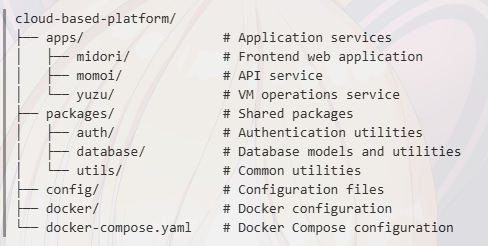
\includegraphics[width=0.8\textwidth]{Image/web/project_structure.png}
% }
% \caption{\fontSixTeen{โครงสร้างโครงงานทั้งหมด}}
% \label{fig4:ProjectStructure}
% \end{figure}

\hspace*{1.3em}
การจัดโครงสร้างโครงงานในลักษณะหลายรีโพซิทอรีนี้ช่วยให้สามารถกำหนดขอบเขตของบริการได้ชัดเจน ลดผลกระทบข้ามระบบเมื่อต้องแก้ไขโค้ด และเหมาะสมกับการดูแลระบบที่มีทั้ง application service และ deployment manifest อยู่ร่วมกันในแพลตฟอร์มเดียว

\section{สถาปัตยกรรมระบบและเทคโนโลยี}
\subsection{การออกแบบสถาปัตยกรรมแบบ Microservices}
\hspace*{1.3em}
ระบบแพลตฟอร์มคลาวด์ที่พัฒนาขึ้นใช้สถาปัตยกรรมแบบ Microservices ซึ่งประกอบด้วยบริการหลัก 3 ตัว คือ Midori, Momoi และ Yuzu โดยมีบริการสนับสนุนเพิ่มเติม เช่น PostgreSQL สำหรับข้อมูลธุรกรรม Redis สำหรับ cache และคิวงาน RustFS สำหรับพื้นที่จัดเก็บไฟล์ และชุด observability สำหรับติดตามสถานะของระบบ แต่ละบริการทำงานอิสระและสื่อสารกันผ่าน HTTP API และระบบคิวงานแบบ asynchronous เพื่อให้ระบบมีความยืดหยุ่นและรองรับการขยายตัวได้ง่าย

\hspace*{1.3em}
เมื่อพิจารณาการทำงานจริงของระบบในคลัสเตอร์ ผู้ใช้จะเริ่มจาก Browser ไปยัง Midori จากนั้น Midori จะเรียก Momoi สำหรับทั้ง API ด้านข้อมูล ตรรกะทางธุรกิจ และการยืนยันตัวตนผ่านเส้นทาง `/api/auth` ขณะที่ Momoi จะทำหน้าที่บันทึกข้อมูลธุรกรรมและส่งงานระยะยาวเข้าสู่ BullMQ บน Redis แล้วให้ Yuzu รับงานไปดำเนินการต่อกับ Proxmox VE รูปแบบนี้ทำให้ API หลักตอบสนองต่อผู้ใช้ได้รวดเร็ว แม้งานโครงสร้างพื้นฐานจะใช้เวลานานและต้อง retry หลายครั้ง

\hspace*{1.3em}
ภาพที่ \ref{fig4:SystemArchitecture} แสดงสถาปัตยกรรมระบบโดยรวม โดยมี \textbf{Midori} เป็นส่วนติดต่อผู้ใช้ที่พัฒนาด้วย Next.js และ React \textbf{Momoi} เป็นบริการ API หลักที่รับผิดชอบตรรกะทางธุรกิจ การเชื่อมต่อฐานข้อมูล และการส่งงานเข้าคิว \textbf{Yuzu} เป็นบริการประมวลผลงานจัดการเครื่องเสมือนที่เชื่อมต่อกับ Proxmox VE และ \textbf{Yuuka} เป็นแหล่งเก็บไฟล์กำหนดค่าการติดตั้งบริการประกอบทั้งหมดของแพลตฟอร์ม

\begin{figure}[H]
\centering
\adjustbox{frame, width=0.75\textwidth}{
    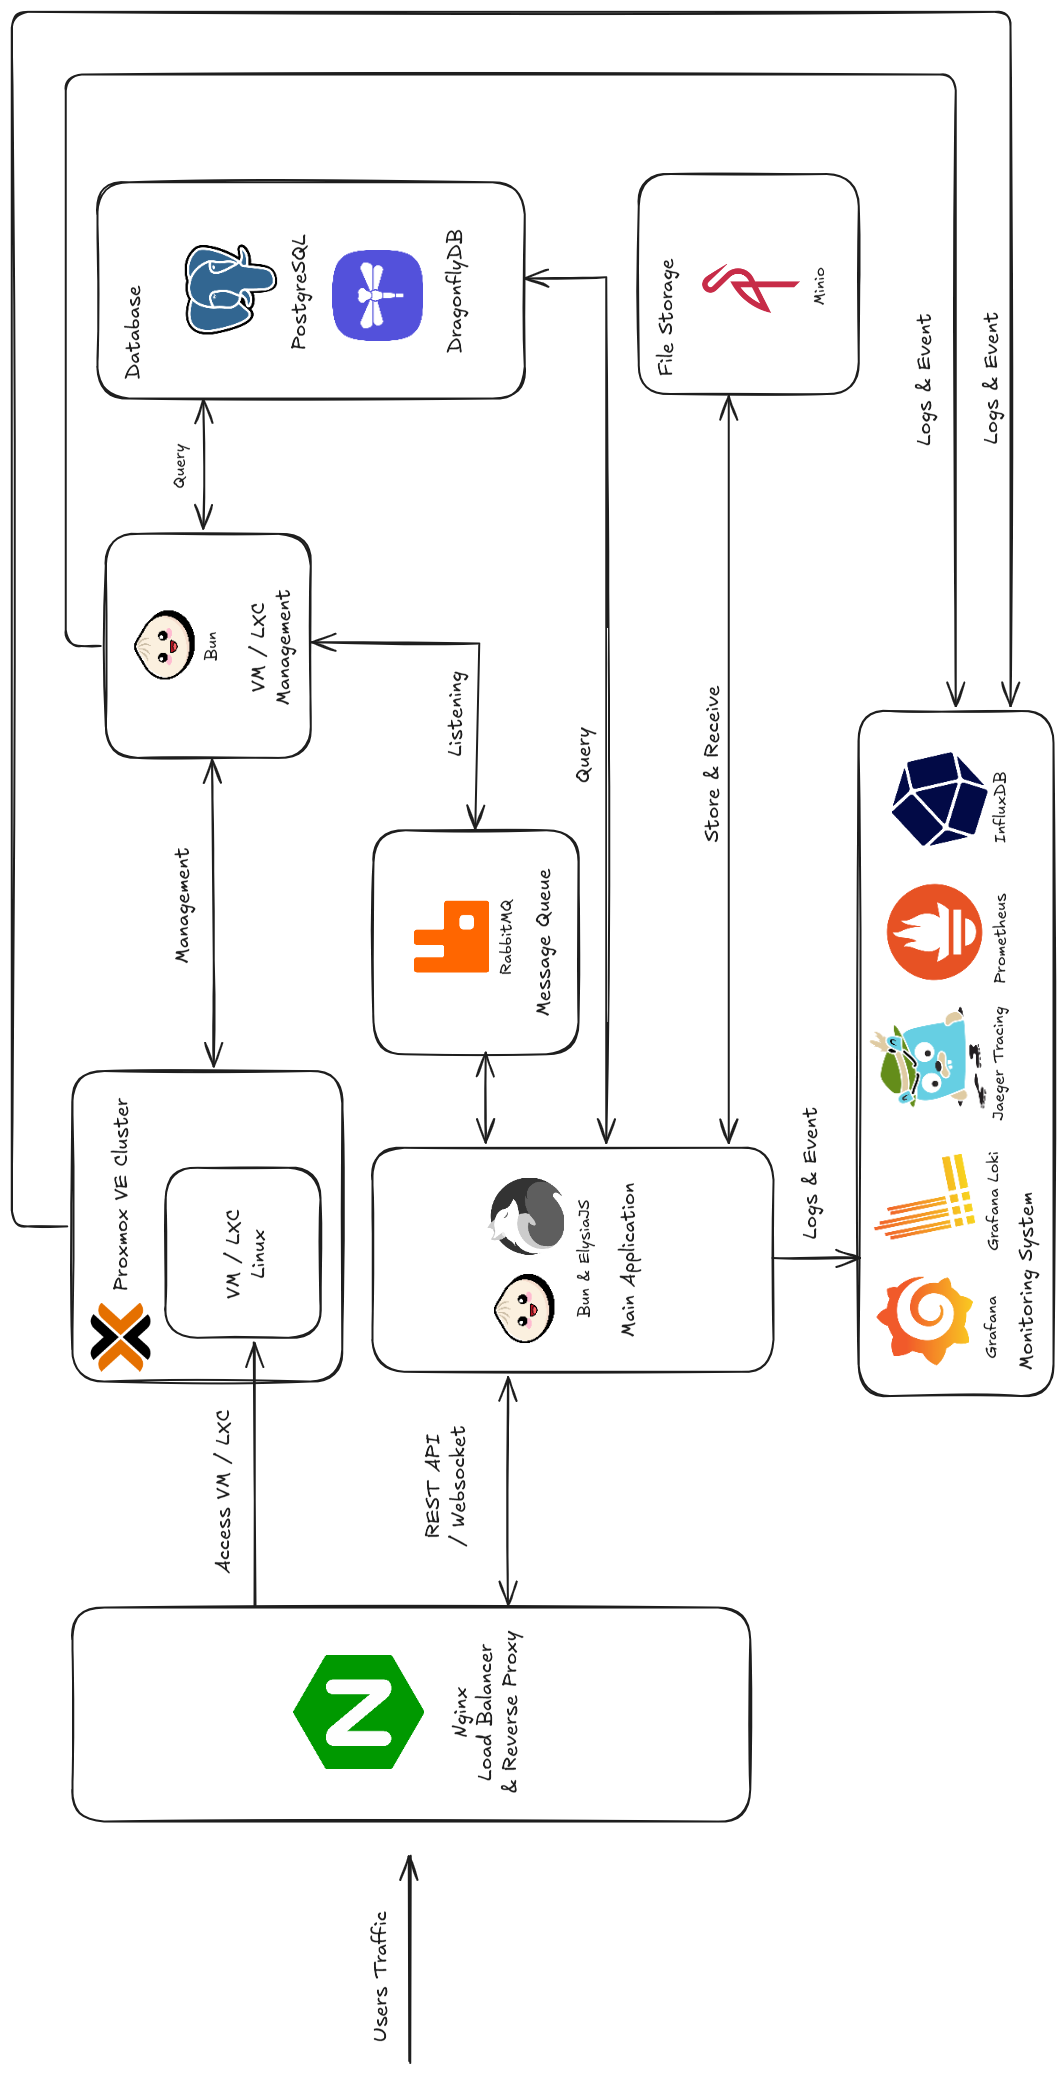
\includegraphics[width=0.75\textwidth]{Image/diagram/system_architecture_90.png}
}
\caption{\fontSixTeen{สถาปัตยกรรมระบบโดยรวม}}
\label{fig4:SystemArchitecture}
\end{figure}

\subsection{เทคโนโลยีที่ใช้ในการพัฒนา}
\hspace*{1.3em}
ในการพัฒนาระบบแพลตฟอร์มคลาวด์นี้ ได้เลือกใช้เทคโนโลยีที่ทันสมัยและเหมาะสมกับการใช้งานในสภาพแวดล้อมการศึกษา โดยเทคโนโลยีหลักที่ใช้ประกอบด้วย
\begin{mycustomitem}
    \item \textbf{Bun Runtime} - JavaScript/TypeScript Runtime ที่มีประสิทธิภาพสูง
    \item \textbf{Next.js 16 และ React 19} - Framework และ Library สำหรับการพัฒนา Frontend
    \item \textbf{Tailwind CSS และ Radix UI} - เครื่องมือสำหรับออกแบบส่วนติดต่อผู้ใช้
    \item \textbf{Elysia.js} - Web Framework สำหรับการพัฒนา API ของ Momoi
    \item \textbf{PostgreSQL} - ระบบจัดการฐานข้อมูลเชิงสัมพันธ์
    \item \textbf{Prisma ORM} - Object-Relational Mapping สำหรับการจัดการฐานข้อมูล
    \item \textbf{Redis และ BullMQ} - ระบบ cache และคิวงาน
    \item \textbf{Docker และ Kubernetes Manifests} - สำหรับการ deploy
    \item \textbf{Prometheus, Grafana, Loki และ Jaeger} - สำหรับการเก็บ metrics, logs และ traces
\end{mycustomitem}

\hspace*{1.3em}
การเลือกใช้เทคโนโลยีเหล่านี้มีเหตุผลสำคัญ คือ ความเสถียร ประสิทธิภาพ และการรองรับการขยายระบบในอนาคต รวมถึงการมี Community ที่ใหญ่และเอกสารประกอบที่ครบถ้วน ทำให้การพัฒนาและบำรุงรักษาระบบเป็นไปอย่างราบรื่น

\section{เอกสารประกอบการใช้งาน API และส่วนติดต่อผู้ใช้}
\subsection{เอกสาร API Documentation}
\hspace*{1.3em}
ระบบแพลตฟอร์มคลาวด์ได้จัดทำเอกสาร API Documentation อย่างครบถ้วนโดยใช้ OpenAPI Specification (Swagger) เพื่อให้ผู้พัฒนาและผู้ใช้งานสามารถเข้าใจและใช้งาน API ได้อย่างง่ายดาย เอกสารนี้ประกอบด้วยรายละเอียดของ Endpoints ต่าง ๆ พารามิเตอร์ที่ต้องการ รูปแบบข้อมูลที่ส่งและรับ รวมทั้งตัวอย่างการใช้งานที่ชัดเจน

\hspace*{1.3em}
ภาพที่ \ref{fig4:APIDocumentation} แสดงหน้าเอกสาร API Documentation ที่สร้างขึ้นโดยอัตโนมัติจากโค้ด TypeScript ผ่าน Elysia.js และ OpenAPI Plugin ซึ่งช่วยให้เห็นโครงสร้างของบริการ Momoi ตามโดเมนงานหลักของระบบ โดยสามารถจัดกลุ่มการใช้งานได้ดังนี้

\begin{mycustomitem}
    \item \textbf{Public API} - สำหรับการใช้งานทั่วไปที่ไม่ต้องมีการยืนยันตัวตน
    \item \textbf{Academic Management API} - สำหรับจัดการรายวิชา ภาคการศึกษา และข้อมูลผู้สอน
    \item \textbf{Request Workflow API} - สำหรับสร้าง ตรวจสอบ และอนุมัติคำร้องขอเครื่องเสมือน
    \item \textbf{Instance API} - สำหรับจัดการเครื่องเสมือนและช่องทางเข้าถึงบริการ
    \item \textbf{Storage API} - สำหรับจัดการไฟล์
\end{mycustomitem}

\begin{figure}[htbp]
\centering
\adjustbox{frame, width=1.0\textwidth}{
    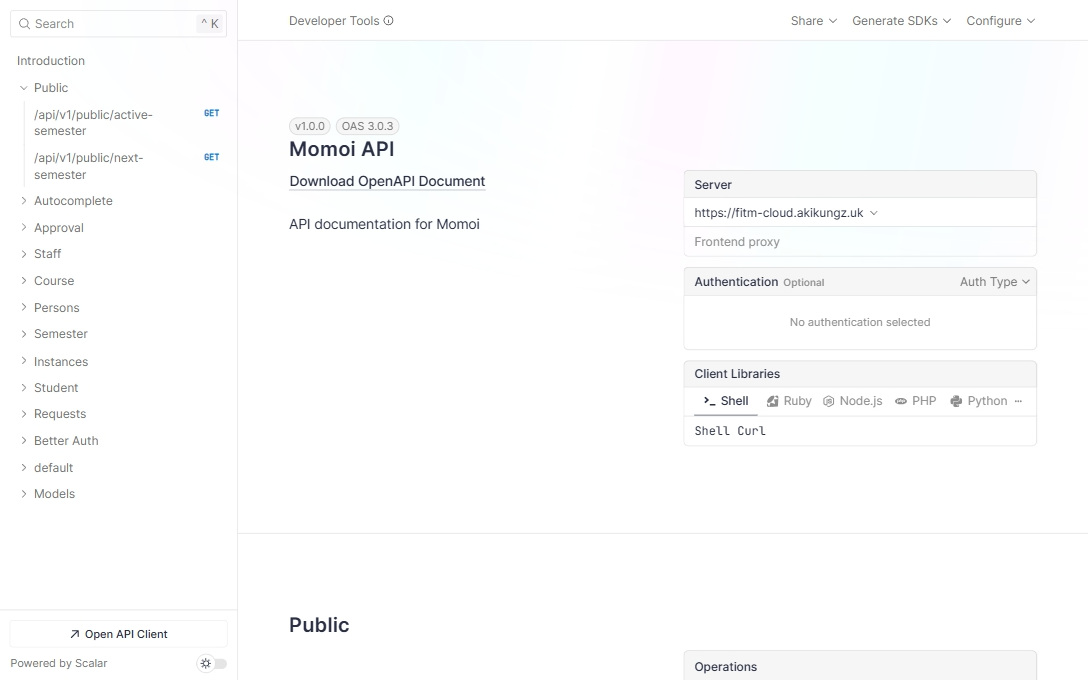
\includegraphics[width=1.0\textwidth]{Image/web/api_documentation.png}
}
\caption{\fontSixTeen{หน้าเอกสาร API Documentation}}
\label{fig4:APIDocumentation}
\end{figure}

\newpage
\hspace*{1.3em}
เอกสาร API นี้มีการอัปเดตอัตโนมัติเมื่อมีการเปลี่ยนแปลงโค้ด และสามารถทดสอบ API ได้โดยตรงผ่านหน้าเว็บ ทำให้ผู้พัฒนาสามารถทำความเข้าใจและใช้งาน API ได้อย่างรวดเร็วและถูกต้อง

\subsection{ส่วนติดต่อผู้ใช้ (User Interface)}
\hspace*{1.3em}
ส่วนติดต่อผู้ใช้ของระบบได้รับการออกแบบให้ใช้งานง่าย สวยงาม และตอบสนองได้ดีบนอุปกรณ์ต่าง ๆ โดยพัฒนาด้วย Next.js, React, Tailwind CSS และชุดองค์ประกอบ UI ที่อิงกับ Radix UI ระบบประกอบด้วยหน้าหลักต่าง ๆ ที่มีการจัดระเบียบข้อมูลและฟังก์ชันการทำงานอย่างชัดเจน ทั้งในส่วนของ dashboard, request workflow, instance management และ storage interface

\hspace*{1.3em}
ภาพที่ \ref{fig4:LandingPage} แสดงหน้าแรกของระบบ (Landing Page) ที่ออกแบบให้ดึงดูดความสนใจและสื่อสารจุดประสงค์ของระบบได้ชัดเจน โดยมีการนำเสนอฟีเจอร์หลักของระบบ ข้อมูลการติดต่อ และลิงก์สำหรับการล็อกอินเข้าสู่ระบบ

\begin{figure}[H]
\centering
\adjustbox{frame, width=0.8\textwidth}{
    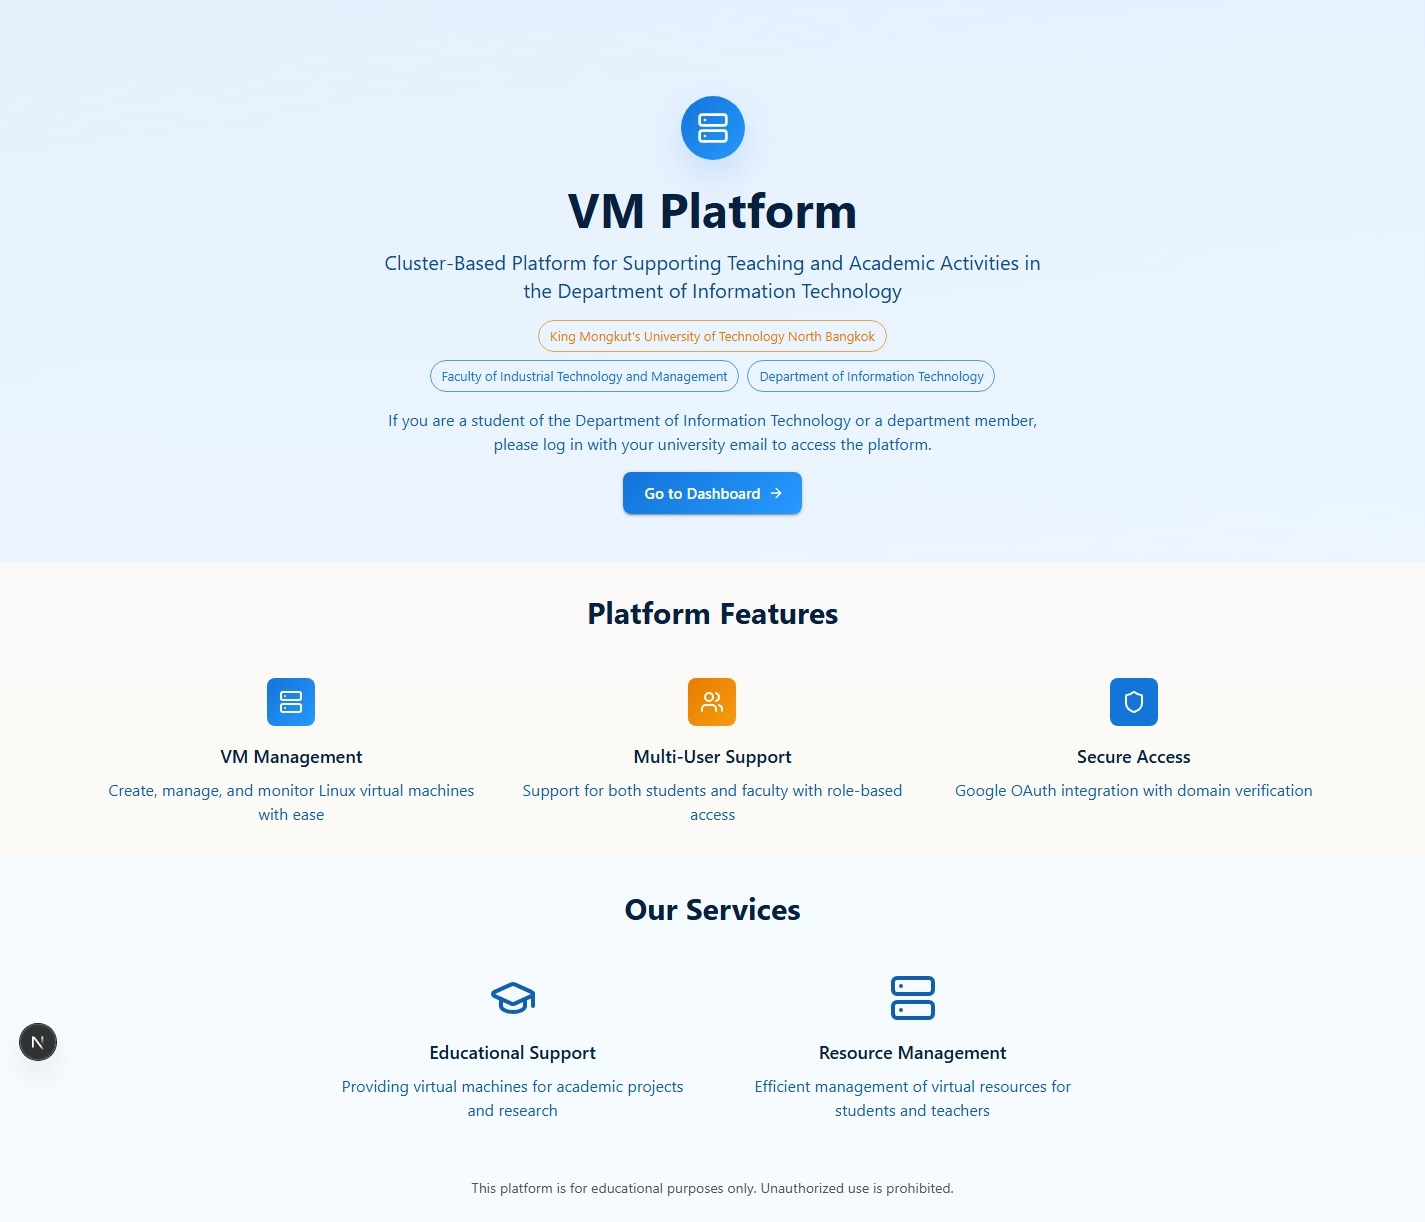
\includegraphics[width=1.0\textwidth]{Image/web/landing_page.jpeg}
}
\caption{\fontSixTeen{หน้าแรกของระบบ (Landing Page)}}
\label{fig4:LandingPage}
\end{figure}

% \newpage
\subsection{Dashboard และระบบจัดการ}
\hspace*{1.3em}
หลังจากที่ผู้ใช้ล็อกอินเข้าสู่ระบบแล้ว ผู้ใช้จะเข้าสู่หน้า Dashboard ที่แสดงข้อมูลสำคัญและฟังก์ชันการทำงานต่าง ๆ ตามบทบาทของผู้ใช้ โดย Dashboard ได้รับการออกแบบให้แสดงข้อมูลอย่างเป็นระบบและเข้าใจง่าย พร้อมทั้งมีการใช้งานที่สะดวกและรวดเร็ว

\hspace*{1.3em}
ส่วนติดต่อผู้ใช้ที่พัฒนาขึ้นมีลักษณะสำคัญดังนี้
\begin{mycustomitem}
    \item \textbf{Responsive Design} - รองรับการแสดงผลบนหน้าจอขนาดต่าง ๆ
    \item \textbf{Intuitive Navigation} - การนำทางที่เข้าใจง่ายและสอดคล้องกับมาตรฐาน UX
    \item \textbf{Role-based UI Visibility} - เมนูและตัวเลือกปรับแสดงผลโดยอัตโนมัติตามบทบาทของผู้ใช้ STUDENT INSTRUCTOR หรือ ADMIN โดยไม่ต้องกำหนดเพิ่มเติม
    \item \textbf{Request Lifecycle Tracking} - แสดงสถานะคำร้องขอตั้งแต่การยื่น การรอพิจารณา จนถึงการอนุมัติหรือปฏิเสธ พร้อม Audit Log ในแต่ละขั้นตอน
    \item \textbf{Instance Control Panel} - แผงควบคุมสถานะเครื่องเสมือน รองรับการสั่ง Start Stop Restart และดูข้อมูล IP และ Reverse Proxy ได้จากหน้าเดียวกัน
    \item \textbf{File Management Interface} - อินเทอร์เฟซสำหรับอัปโหลด จัดโฟลเดอร์ และกำหนดสิทธิ์การแบ่งปันไฟล์ภายในแพลตฟอร์ม
\end{mycustomitem}

\hspace*{1.3em}
การออกแบบส่วนติดต่อผู้ใช้ได้คำนึงถึงประสบการณ์ผู้ใช้ (User Experience) เป็นหลัก โดยมุ่งเน้นให้ผู้ใช้สามารถทำงานได้อย่างมีประสิทธิภาพและลดข้อผิดพลาดในการใช้งาน ทั้งนี้ระบบยังมีการจัดการข้อผิดพลาดและการแจ้งเตือนที่ชัดเจน เพื่อให้ผู้ใช้สามารถแก้ไขปัญหาได้อย่างรวดเร็ว

\section{ตัวอย่างการใช้งานระบบตามบทบาทผู้ใช้}
\subsection{Dashboard สำหรับนักศึกษา}
\hspace*{1.3em}
ระบบได้จัดทำ Dashboard เฉพาะสำหรับนักศึกษา เพื่อให้สามารถจัดการเครื่องเสมือนส่วนตัวและติดตามการใช้งานทรัพยากรได้อย่างง่ายดาย ภาพที่ \ref{fig4:StudentDashboard} แสดง Dashboard หลักของนักศึกษาที่ประกอบด้วยข้อมูลสรุปการใช้งาน สถานะเครื่องเสมือน และฟังก์ชันการจัดการที่สำคัญ

\begin{figure}[H]
\centering
\adjustbox{frame, width=0.8\textwidth}{
    
\includegraphics[width=1.0\textwidth]{Image/web/dashboard/student/dashboard.jpeg}
}
\caption{\fontSixTeen{Dashboard หลักสำหรับนักศึกษา}}
\label{fig4:StudentDashboard}
\end{figure}

\hspace*{1.3em}
นักศึกษาสามารถดูรายการเครื่องเสมือนทั้งหมดที่ตนเองมีสิทธิ์เข้าถึง พร้อมทั้งสถานะการทำงาน การใช้ทรัพยากร และการจัดการพื้นฐาน ดังแสดงในภาพที่ \ref{fig4:StudentInstances} ซึ่งนำเสนอรายละเอียดของแต่ละ Instance อย่างชัดเจน

\begin{figure}[H]
\centering
\adjustbox{frame, width=0.8\textwidth}{
    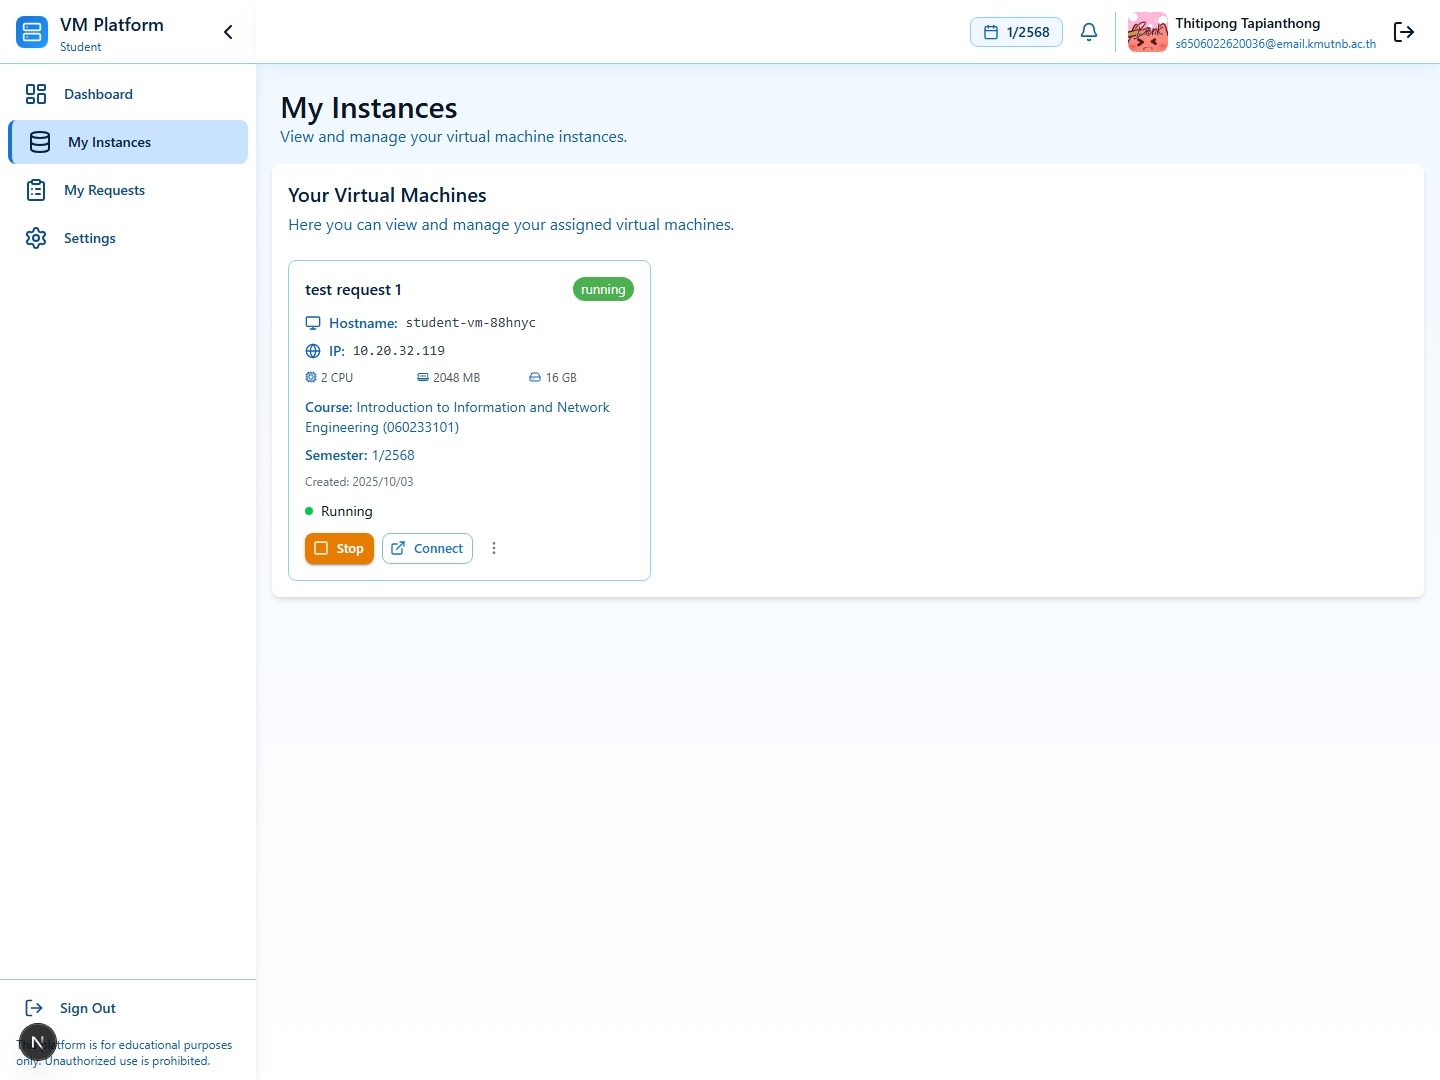
\includegraphics[width=1.0\textwidth]{Image/web/dashboard/student/instances.jpeg}
}
\caption{\fontSixTeen{หน้าจัดการ VM Instances สำหรับนักศึกษา}}
\label{fig4:StudentInstances}
\end{figure}

\hspace*{1.3em}
นอกจากนี้ นักศึกษายังสามารถขอสร้างเครื่องเสมือนใหม่ผ่านฟอร์มที่ออกแบบมาอย่างเรียบง่าย ดังแสดงในภาพที่ \ref{fig4:StudentCreateInstance} ซึ่งช่วยให้การขอใช้ทรัพยากรเป็นไปอย่างรวดเร็วและมีประสิทธิภาพ

\begin{figure}[H]
\centering
\adjustbox{frame, width=0.8\textwidth}{
    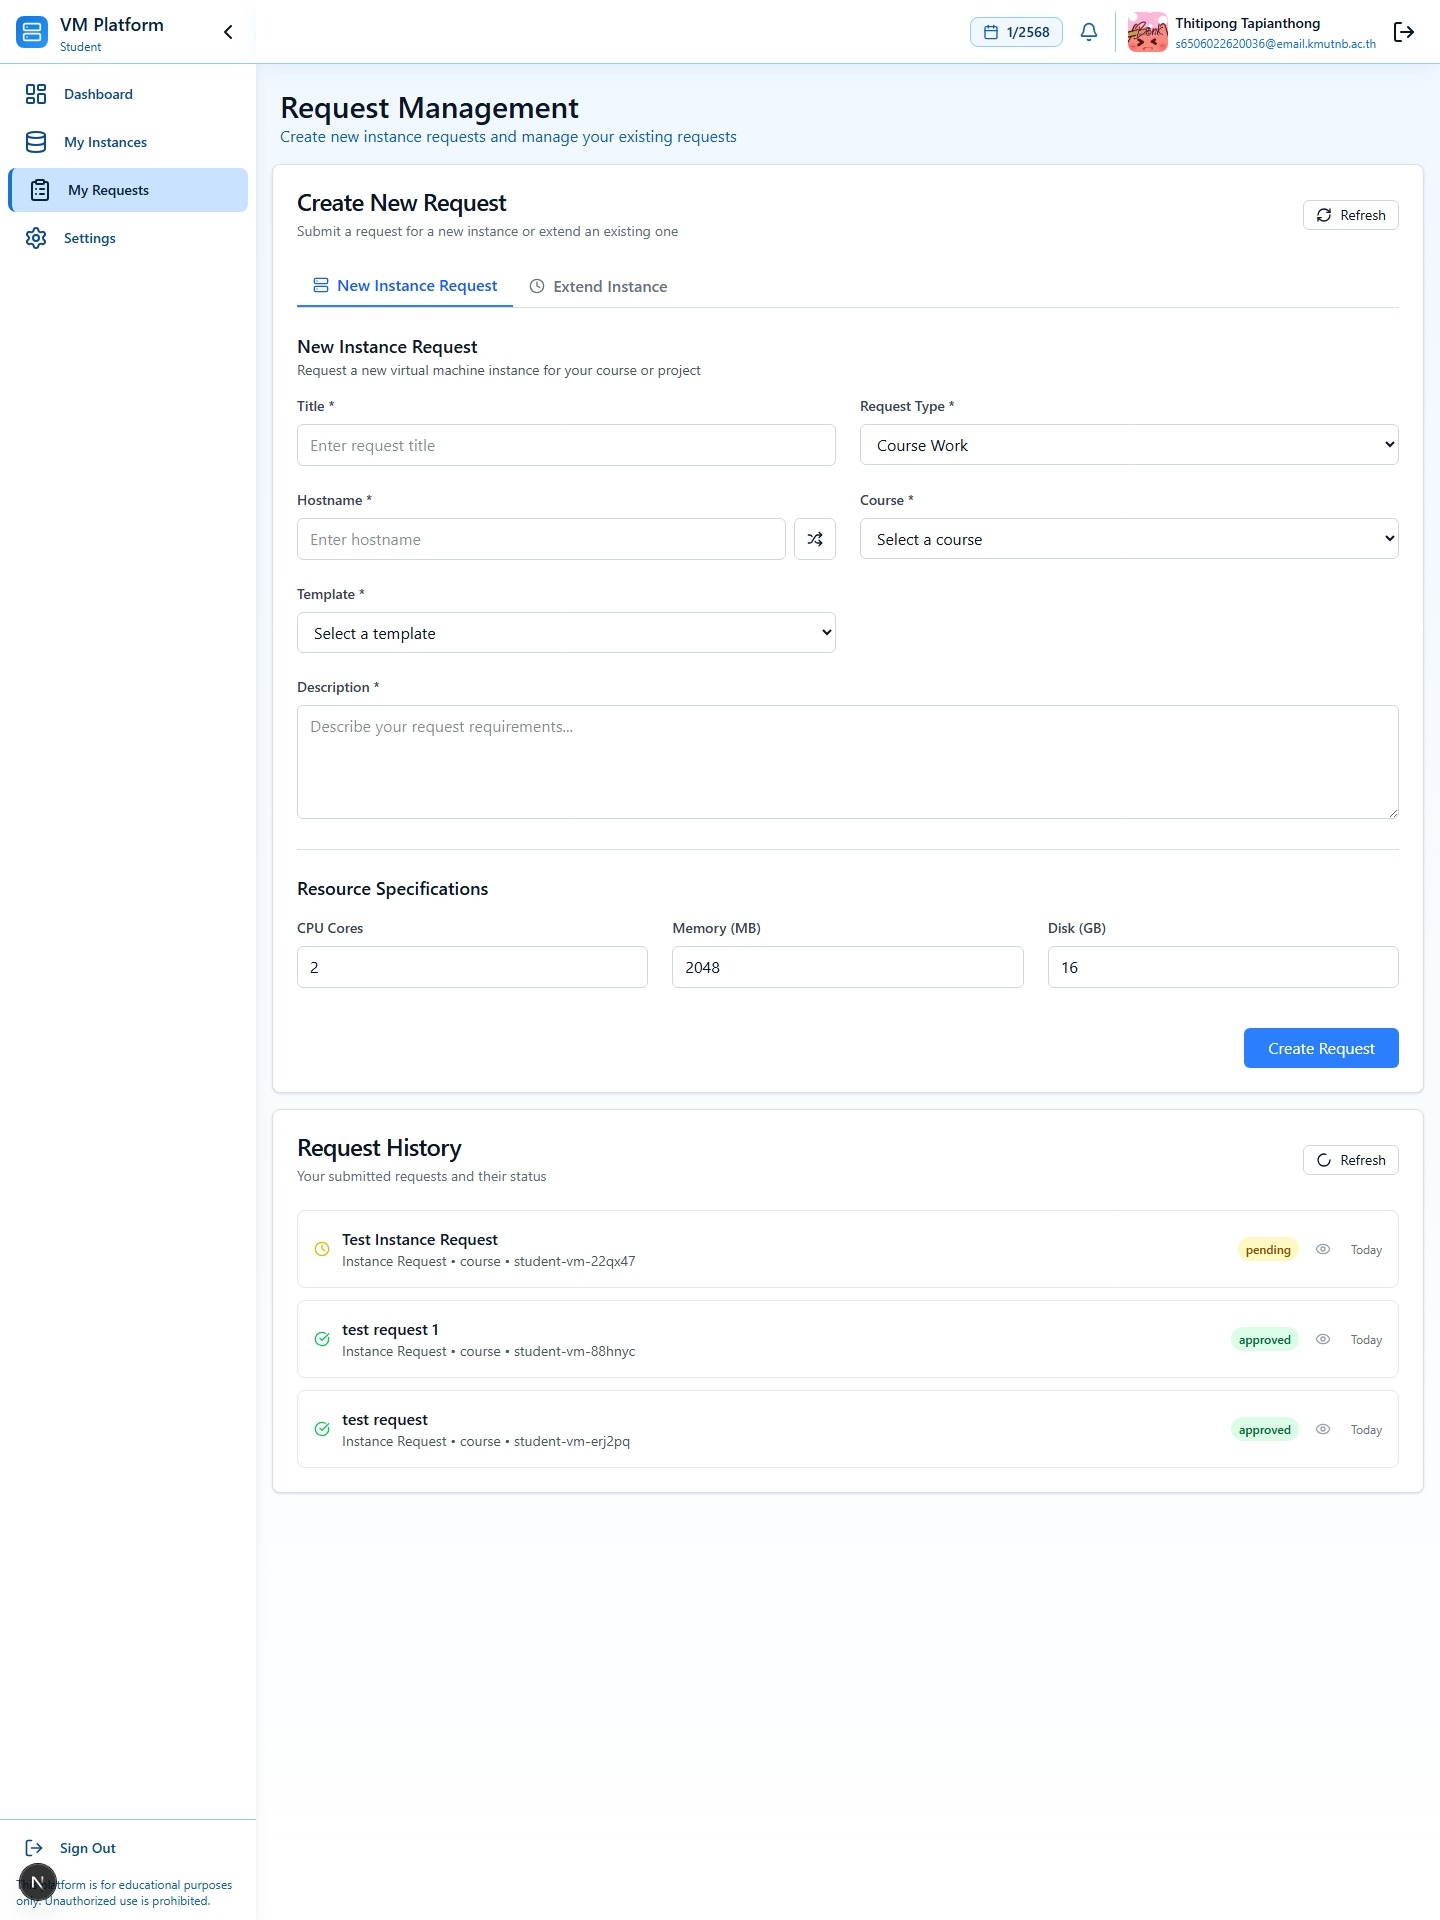
\includegraphics[width=1.0\textwidth]{Image/web/dashboard/student/requests.jpeg}
}
\caption{\fontSixTeen{หน้าจอขอสร้าง VM Instance ใหม่สำหรับนักศึกษา}}
\label{fig4:StudentCreateInstance}
\end{figure}

\newpage
\subsection{Dashboard สำหรับอาจารย์และเจ้าหน้าที่}
\hspace*{1.3em}
สำหรับอาจารย์และเจ้าหน้าที่ ระบบได้จัดเตรียม Dashboard ที่มีฟังก์ชันการจัดการขั้นสูงมากขึ้น รวมถึงการอนุมัติคำขอ การจัดการหลักสูตร และการตรวจสอบการใช้งานของนักศึกษา ภาพที่ \ref{fig4:StaffDashboard} แสดง Dashboard หลักสำหรับเจ้าหน้าที่ที่มีข้อมูลสถิติและการควบคุมระบบ

\begin{figure}[H]
\centering
\adjustbox{frame, width=0.8\textwidth}{
    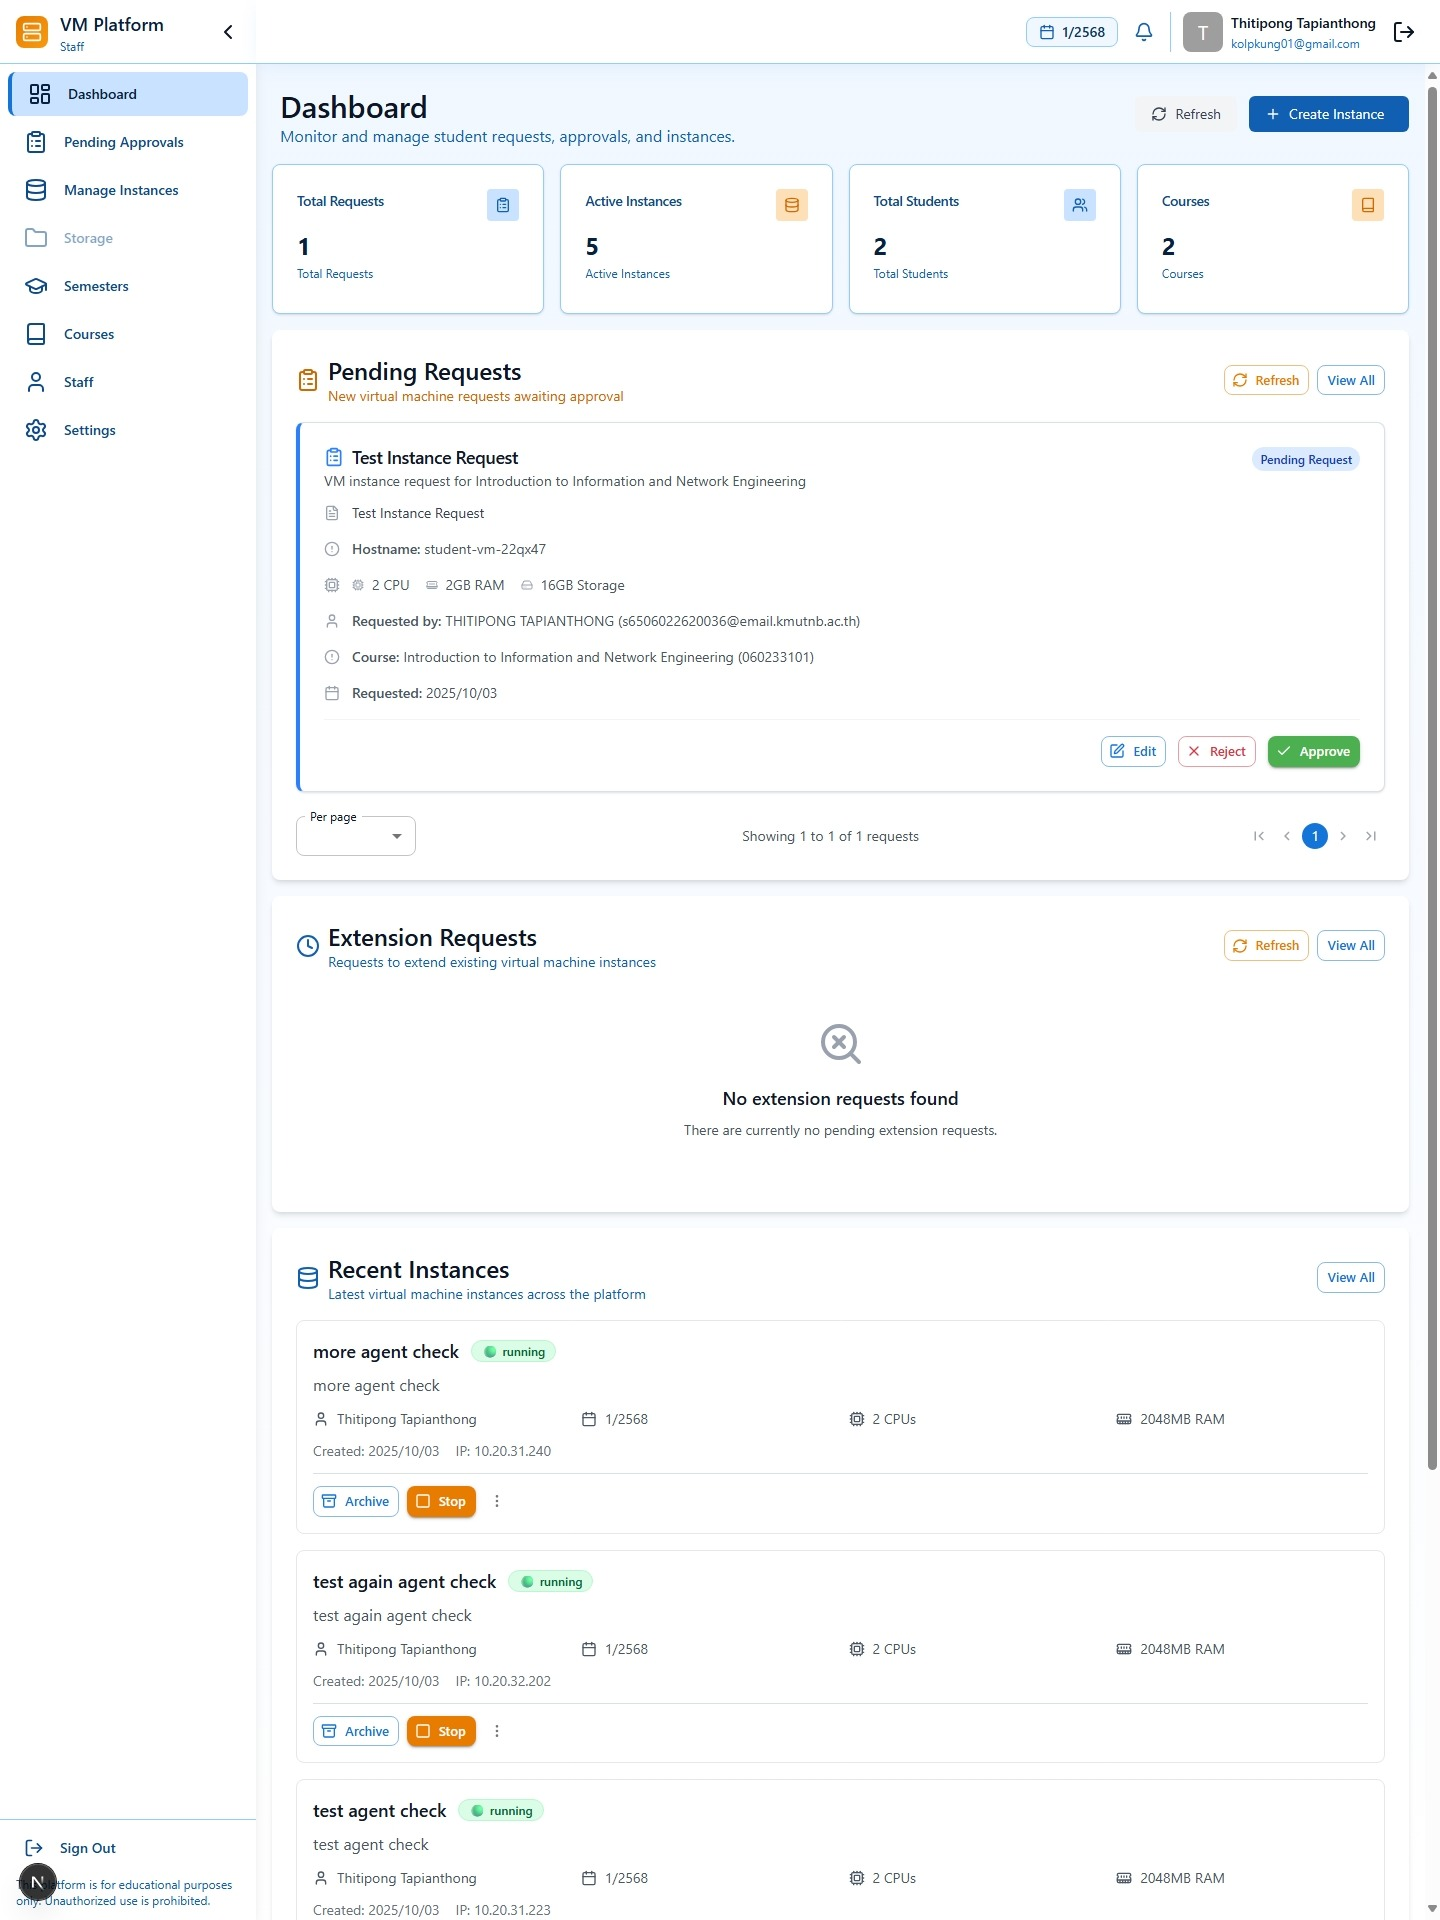
\includegraphics[width=1.0\textwidth]{Image/web/dashboard/staff/dashboard.jpeg}
}
\caption{\fontSixTeen{Dashboard หลักสำหรับอาจารย์และเจ้าหน้าที่}}
\label{fig4:StaffDashboard}
\end{figure}

\hspace*{1.3em}
อาจารย์และเจ้าหน้าที่สามารถจัดการหลักสูตร เทอมการศึกษา รวมถึงการจัดการรายชื่อของอาจารย์และเจ้าหน้าที่ ดังแสดงในภาพที่ \ref{fig4:CourseManagement} - \ref{fig4:StaffManagement} ซึ่งช่วยให้สามารถกำหนดทรัพยากรและสิทธิ์การเข้าถึงสำหรับแต่ละวิชาได้อย่างเหมาะสม

\begin{figure}[H]
\centering
\adjustbox{frame, width=0.8\textwidth}{
    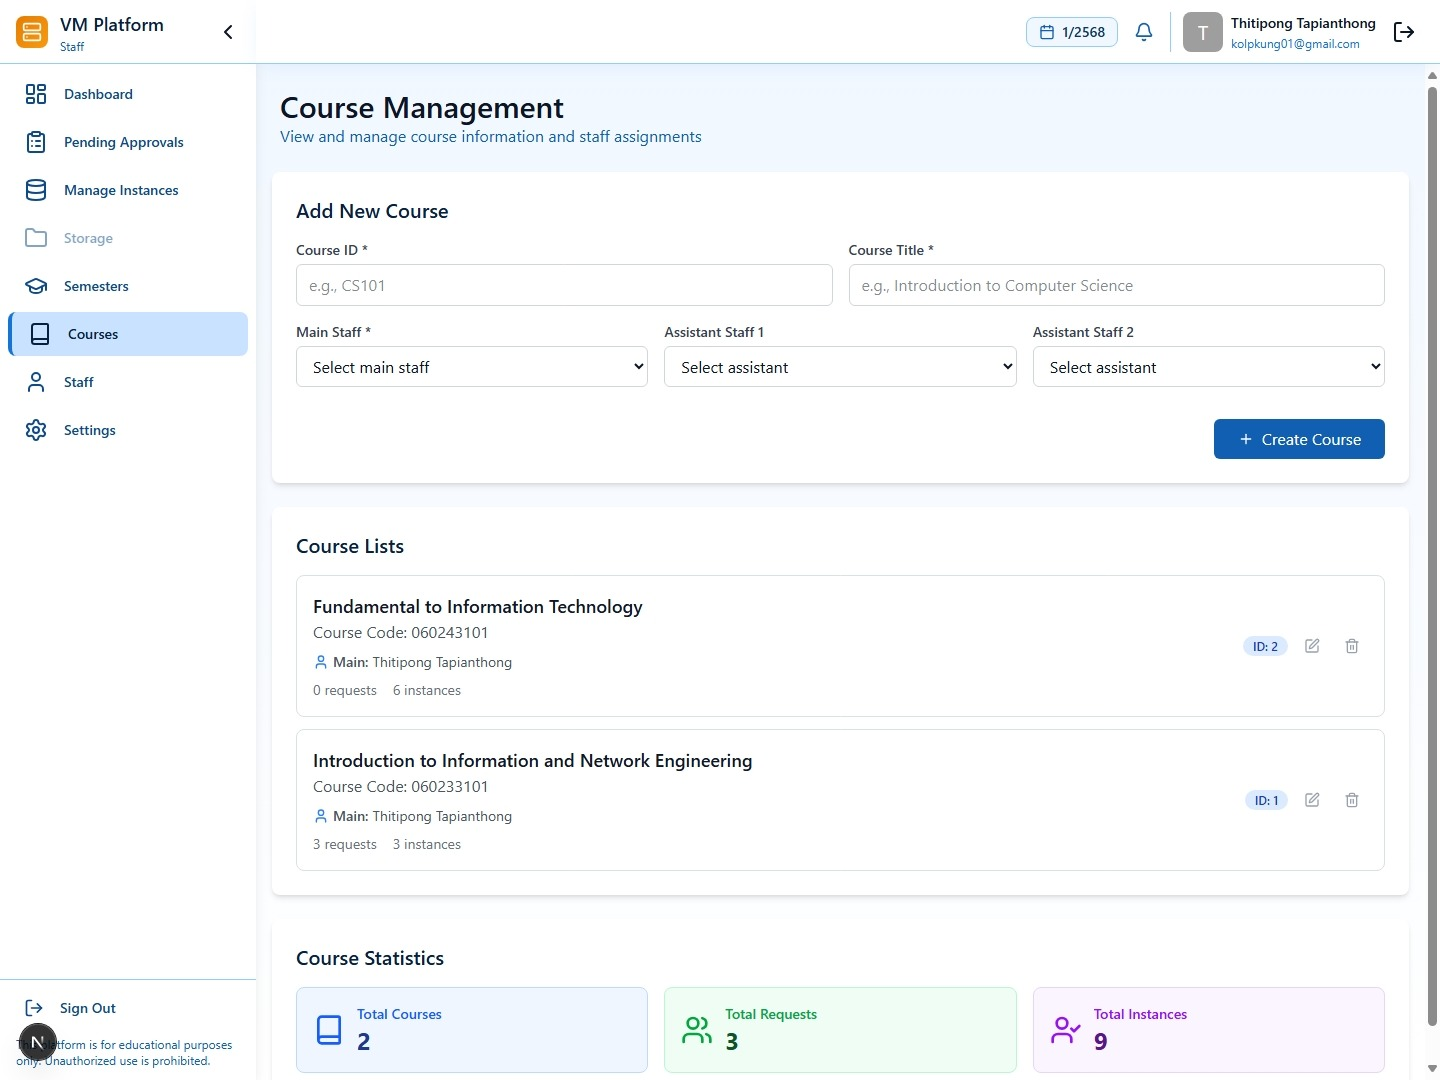
\includegraphics[width=0.8\textwidth]{Image/web/dashboard/staff/courses.jpeg}
}
\caption{\fontSixTeen{หน้าจัดการหลักสูตรและรายวิชา}}
\label{fig4:CourseManagement}
\end{figure}

\begin{figure}[H]
\centering
\adjustbox{frame, width=0.8\textwidth}{
    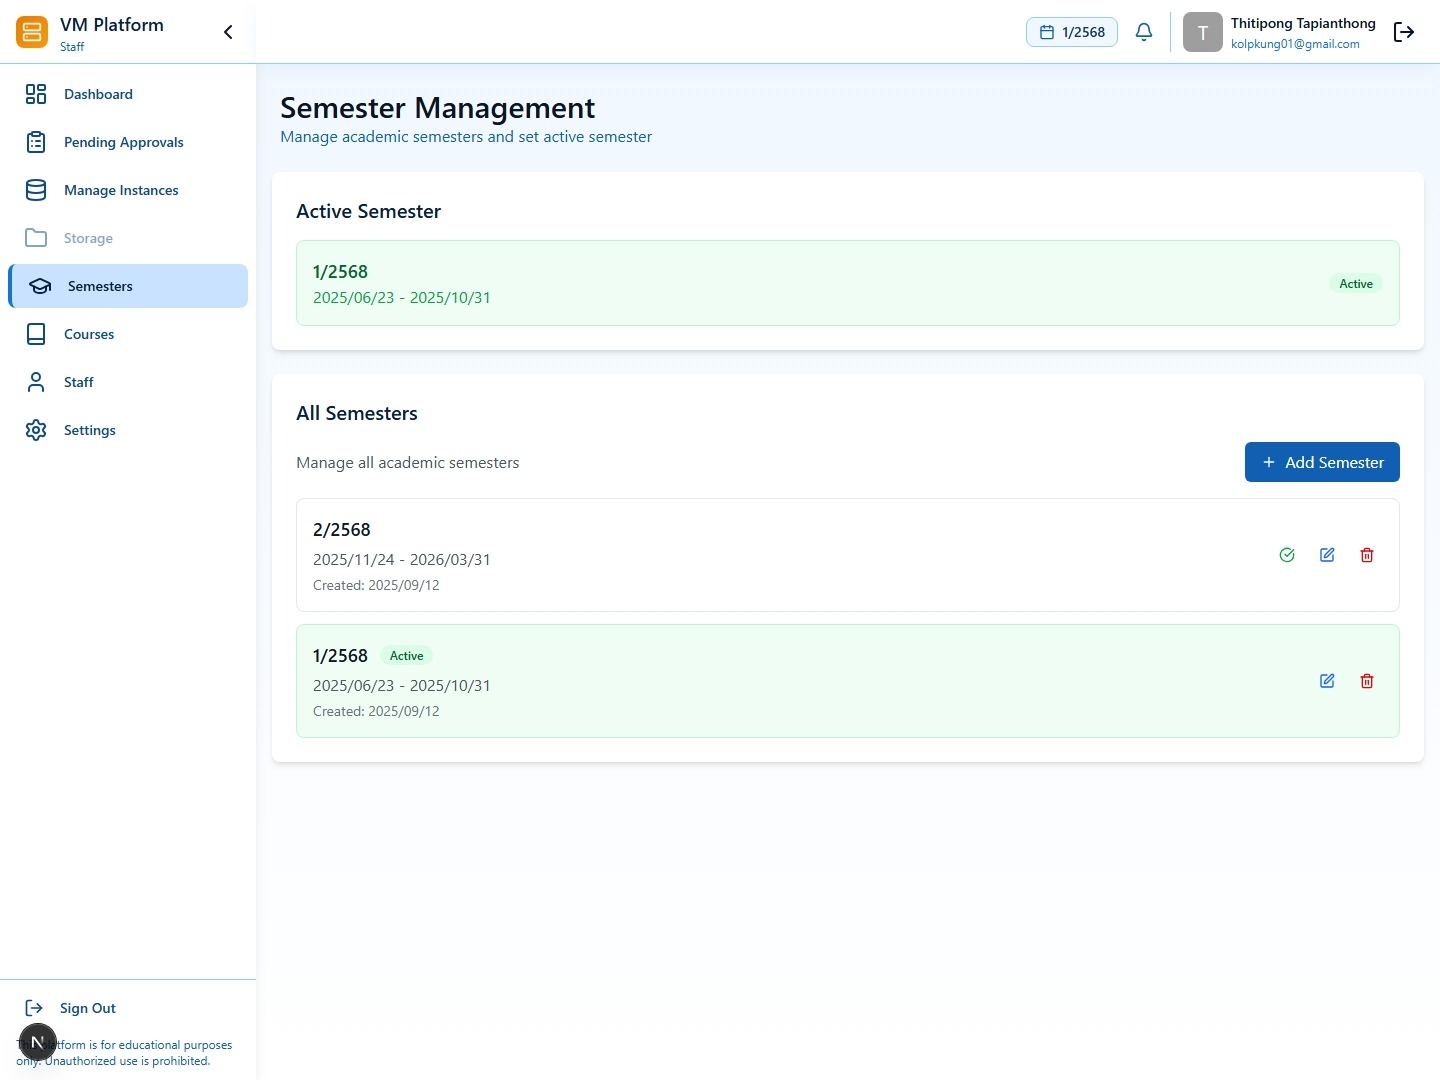
\includegraphics[width=0.8\textwidth]{Image/web/dashboard/staff/semesters.jpeg}
}
\caption{\fontSixTeen{หน้าจัดการเทอมการศึกษา}}
\label{fig4:SemesterManagement}
\end{figure}

\begin{figure}[H]
\centering
\adjustbox{frame, width=0.8\textwidth}{
    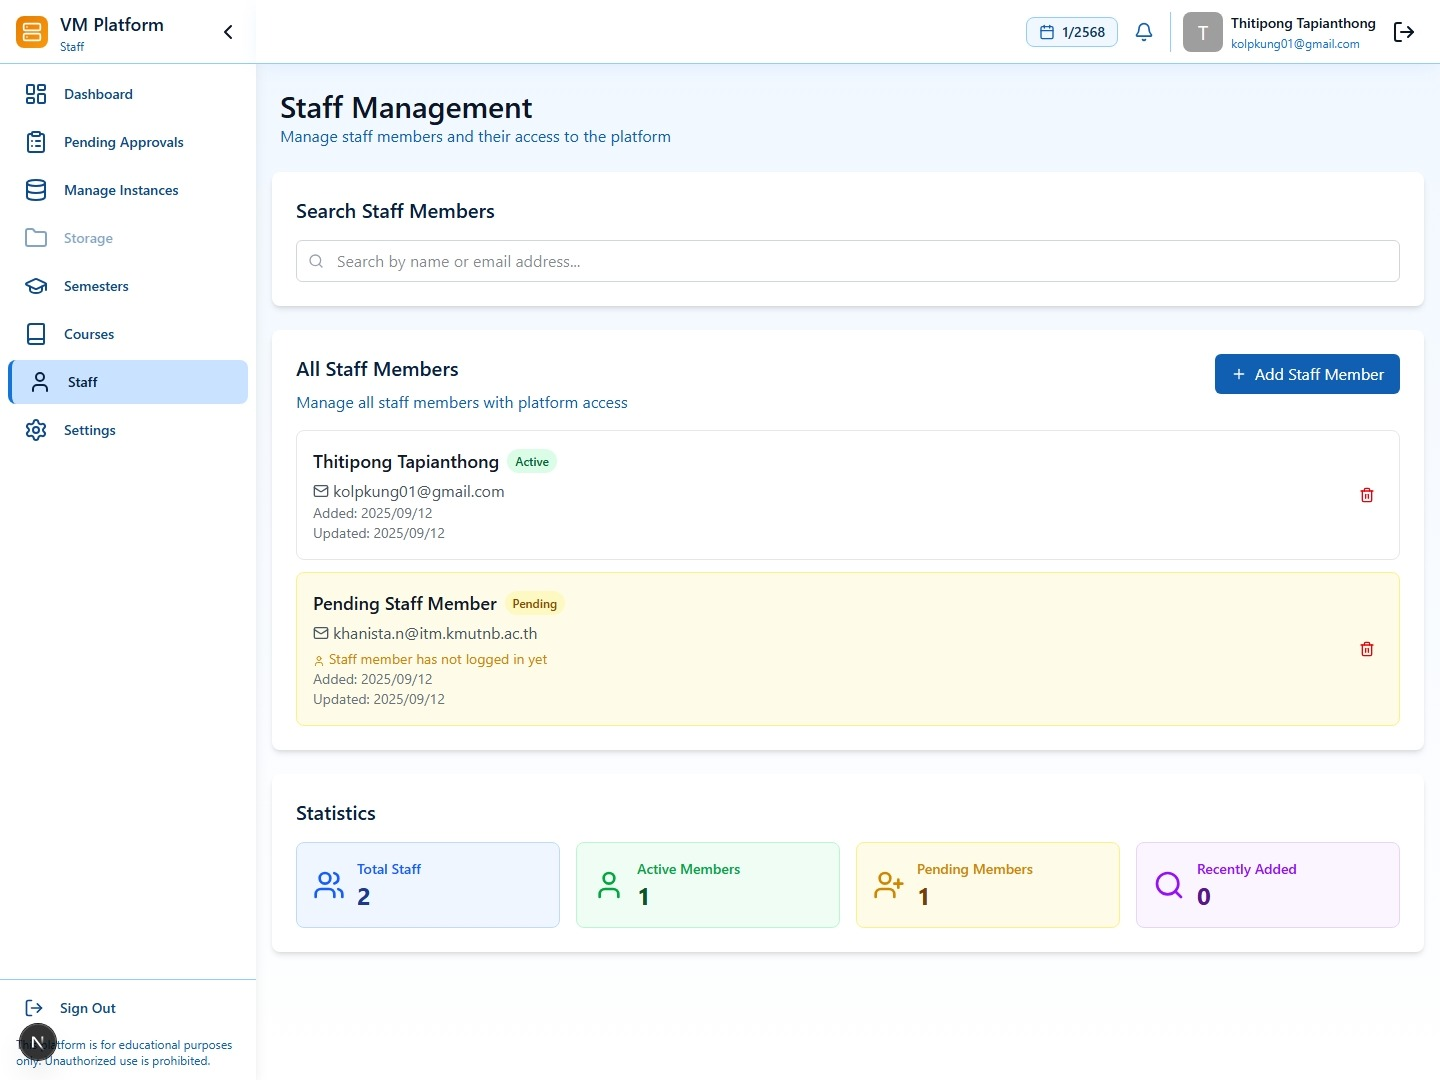
\includegraphics[width=0.8\textwidth]{Image/web/dashboard/staff/staff_management.jpeg}
}
\caption{\fontSixTeen{หน้าจัดการรายชื่ออาจารย์}}
\label{fig4:StaffManagement}
\end{figure}

\hspace*{1.3em}
นอกจากนี้ ระบบยังมีหน้าสำหรับการอนุมัติคำขอต่าง ๆ จากนักศึกษา ดังแสดงในภาพที่ \ref{fig4:PendingApproval} ซึ่งช่วยให้อาจารย์สามารถตรวจสอบและอนุมัติคำขอได้อย่างมีประสิทธิภาพ

\begin{figure}[H]
\centering
\adjustbox{frame, width=0.8\textwidth}{
    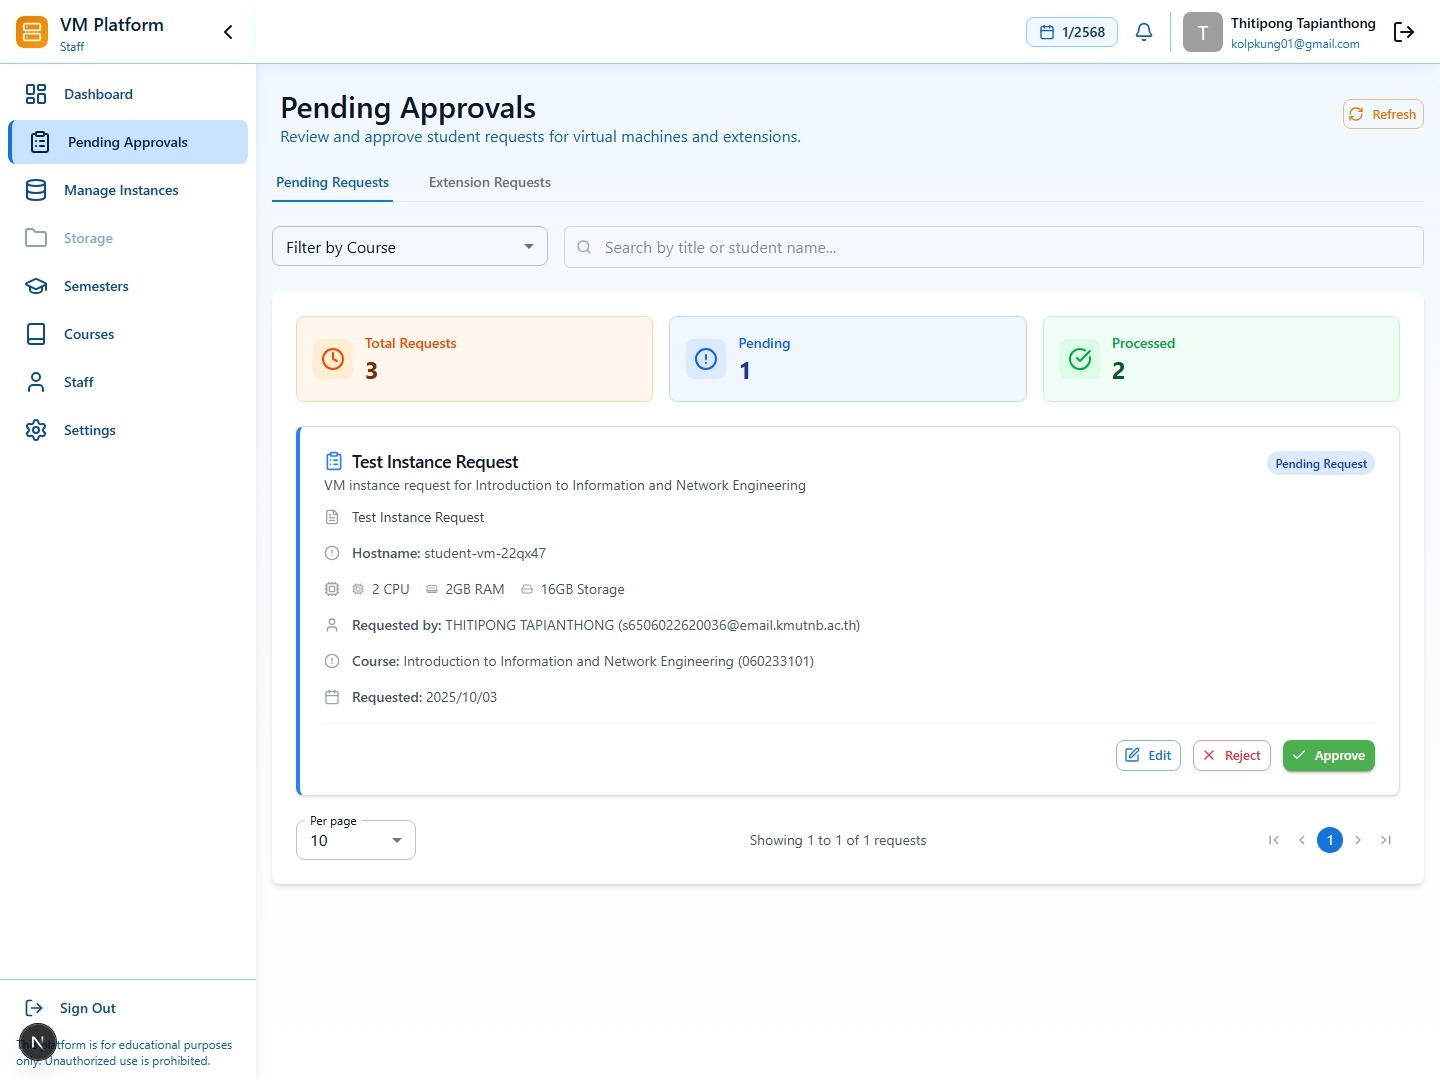
\includegraphics[width=0.8\textwidth]{Image/web/dashboard/staff/pending_approval.jpeg}
}
\caption{\fontSixTeen{หน้าอนุมัติคำขอที่รอดำเนินการ}}
\label{fig4:PendingApproval}
\end{figure}

% \newpage
\subsection{ระบบจัดการแบบ Role-Based Access Control}
\hspace*{1.3em}
ระบบได้นำเอา Role-Based Access Control (RBAC) มาใช้ในการจัดการสิทธิ์การเข้าถึงข้อมูลและฟังก์ชันต่าง ๆ โดยแบ่งผู้ใช้เป็น 3 กลุ่มหลัก คือ นักศึกษา อาจารย์ และผู้ดูแลระบบ ซึ่งแต่ละกลุ่มจะมีสิทธิ์และหน้าที่ที่แตกต่างกันตามความเหมาะสม

\hspace*{1.3em}
การออกแบบระบบในลักษณะนี้ช่วยให้การจัดการความปลอดภัยของข้อมูลเป็นไปอย่างมีประสิทธิภาพ และผู้ใช้แต่ละกลุ่มจะเห็นเฉพาะข้อมูลและฟังก์ชันที่เกี่ยวข้องกับหน้าที่ของตนเอง ทำให้การใช้งานง่ายขึ้นและลดความเสี่ยงในการเข้าถึงข้อมูลที่ไม่เหมาะสม

\section{ระบบติดตามและสังเกตการณ์การทำงาน (Observability)}
\hspace*{1.3em}
ระบบได้ติดตั้งชุดเครื่องมือสำหรับสังเกตการณ์การทำงาน (Observability Stack) โดยใช้ \textbf{Prometheus} สำหรับเก็บ metrics จากบริการหลัก \textbf{Grafana} สำหรับแสดงผลบนหน้า dashboard \textbf{Loki} สำหรับรวบรวมและค้นหา application log และ \textbf{Jaeger} สำหรับ distributed tracing ข้ามบริการ ทำให้ผู้ดูแลระบบสามารถติดตามสถานะและวิเคราะห์ปัญหาได้แบบ real-time

\subsection{ผลการติดตามบน Grafana Dashboard}
\hspace*{1.3em}
แต่ละบริการหลักมีรูปแบบการสังเกตการณ์ที่แตกต่างกันตามบทบาทของตนเอง โดย Midori และ Momoi มีการส่ง traces ไปยัง Jaeger ผ่าน OpenTelemetry และมี metrics endpoint สำหรับ Prometheus ส่วน Yuzu เน้นการเปิดเผย metrics และ structured logs ของ queue worker และการเรียกใช้งาน Proxmox VE ผ่าน Prometheus-compatible endpoint ของตนเอง ตัวชี้วัดหลักที่ติดตาม ได้แก่ อัตราคำขอต่อวินาที latency percentile (p50, p95, p99) สถานะของ queue worker จำนวนงานในคิว เวลาในการทำ provision และอัตราความสำเร็จของการจัดสรรเครื่องเสมือน ข้อมูลเหล่านี้จะถูกนำเสนอใน Grafana dashboard ที่ออกแบบแยกตามบริการ และรวมไว้ในหน้าภาพรวมของระบบทั้งหมด

\hspace*{1.3em}
ภาพที่ \ref{fig4:MonitoringDashboard} แสดงตัวอย่างผลการติดตามบน Grafana ซึ่งช่วยให้ผู้ดูแลระบบเห็นภาพรวมของสถานะบริการและแนวโน้มของตัวชี้วัดสำคัญได้ในหน้าเดียว

\begin{figure}[H]
\centering
\adjustbox{frame, width=0.5\textwidth}{
    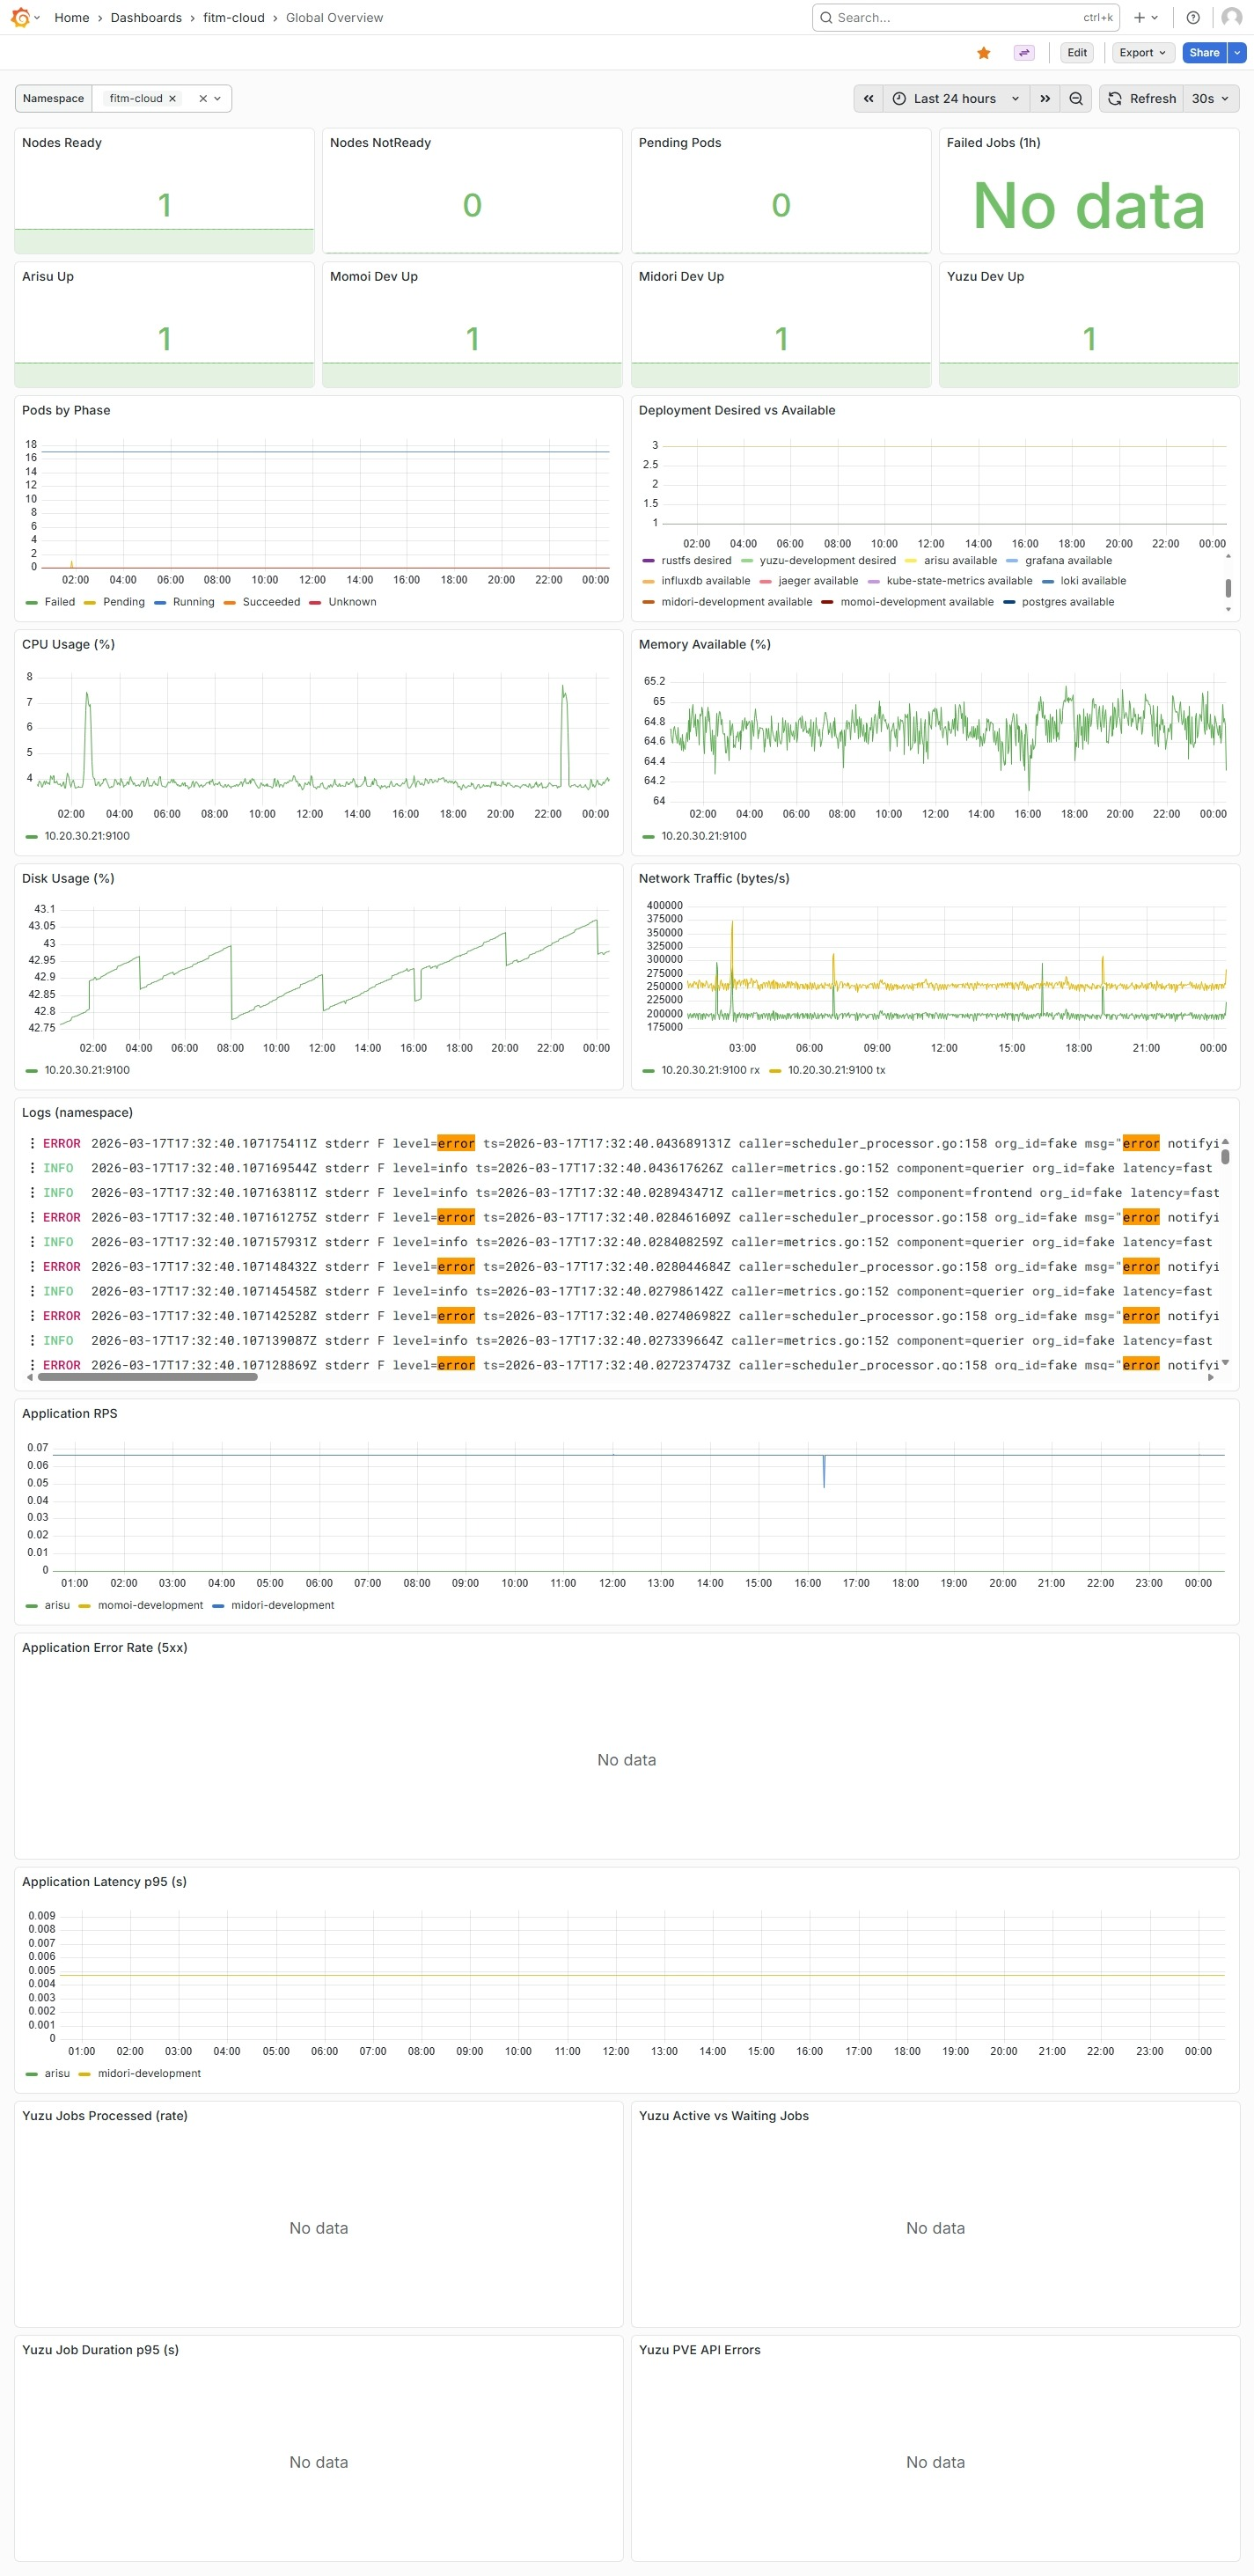
\includegraphics[width=1.0\textwidth]{Image/monitoring_dashboard.jpeg}
}
\caption{\fontSixTeen{ตัวอย่างผลการติดตามสถานะระบบบน Grafana Dashboard}}
\label{fig4:MonitoringDashboard}
\end{figure}

\subsection{ผลการติดตามแบบ Distributed Tracing ด้วย Jaeger}
\hspace*{1.3em}
Jaeger ถูกนำมาใช้เพื่อ trace การประมวลผลคำขอในเส้นทางที่เกี่ยวข้องกับ Midori และ Momoi ซึ่งช่วยในการระบุคอขวดและวิเคราะห์ latency ระหว่าง frontend และ API ได้อย่างมีประสิทธิภาพ สำหรับกระบวนการสร้างเครื่องเสมือนที่ต่อเนื่องไปยัง Redis Queue และ Yuzu นั้น ปัจจุบันการติดตามฝั่ง worker ยังพึ่งพา metrics และ logs มากกว่าการ trace แบบ end-to-end เต็มรูปแบบ ดังนั้นการวิเคราะห์ความล่าช้าในช่วงปฏิบัติการบน Proxmox VE จะอาศัยข้อมูลจาก queue metrics, worker logs และสถานะงานร่วมกัน

\hspace*{1.3em}
ภาพที่ \ref{fig4:MonitoringTrace} แสดงตัวอย่าง trace ที่รวบรวม span ของการประมวลผลคำขอในแต่ละชั้นบริการ ทำให้สามารถตรวจสอบขั้นตอนที่ใช้เวลามากผิดปกติและช่วยวิเคราะห์สาเหตุของความล่าช้าได้อย่างเป็นระบบ

\begin{figure}[H]
\centering
\adjustbox{frame, width=1.0\textwidth}{
    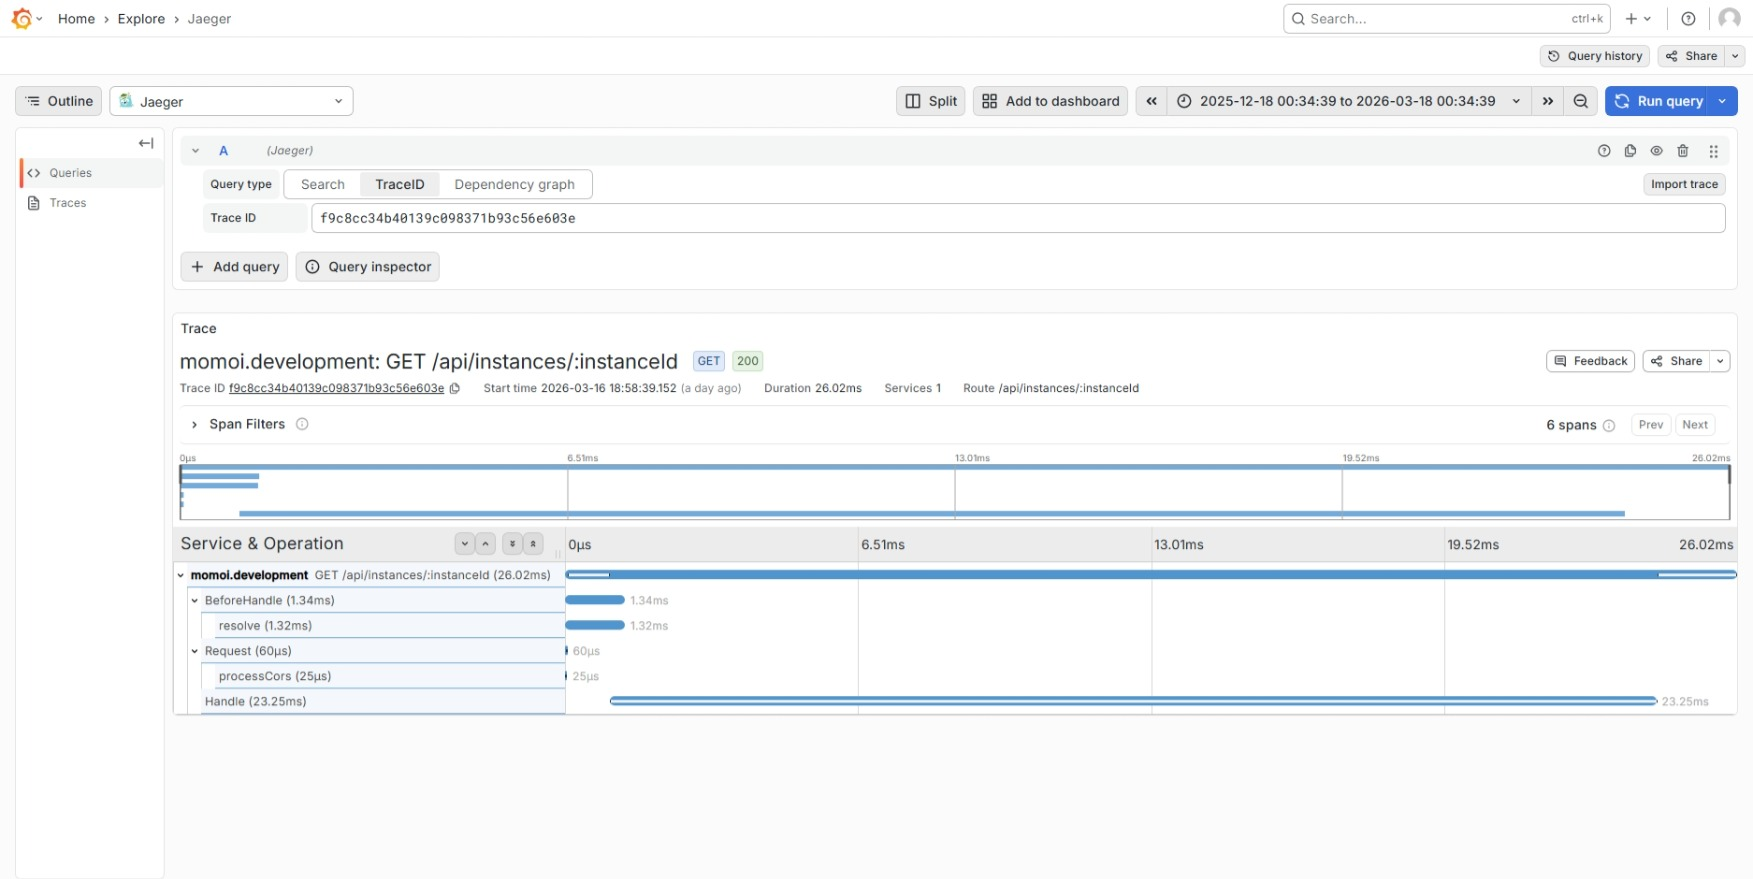
\includegraphics[width=1.0\textwidth]{Image/monitoring_dashboard_trace.jpeg}
}
\caption{\fontSixTeen{ตัวอย่างผลการติดตามเส้นทางคำขอ (Trace) บน Jaeger}}
\label{fig4:MonitoringTrace}
\end{figure}

\section{ผลการทดสอบประสิทธิภาพระบบ}
\label{sec:system-perf}
\hspace*{1.3em}
ส่วนนี้สรุปผลการทดสอบประสิทธิภาพของบริการหลักในระบบ โดยแบ่งตามบริการย่อย เพื่อให้เห็นภาพรวมและเปรียบเทียบสมรรถนะของแต่ละบริการได้อย่างชัดเจน

\subsection{ผลการทดสอบประสิทธิภาพส่วนติดต่อผู้ใช้ (Midori)}
\label{sec:midori-perf}
\hspace*{1.3em}
ทำการทดสอบสมรรถนะของ \textbf{Midori} (Frontend/Next.js) โดยมีเป้าหมายการทดสอบคือ \url{https://dev.fitm.cloud} ระยะเวลารวม 30 วินาที และระดับความขนานต่อเส้นทาง (Path-Level Parallelism) 100 พร้อมทั้งบันทึกรายละเอียดคำขอรายครั้งลงในไฟล์ log เพื่อใช้วิเคราะห์ความสม่ำเสมอของเวลาตอบสนองและพฤติกรรมในช่วง tail latency

\hspace*{1.3em}
ภาพรวมของการทดสอบสะท้อนปริมาณคำขอรวม 3{,}506 คำขอ อัตราความสำเร็จ 96.55\% และอัตราการส่งผ่านโดยเฉลี่ย 109.67 RPS ดังตารางที่ \ref{tab:midori-summary}

\begin{table}[htbp]
    \centering
    \caption{\fontSixTeen{สรุปผลภาพรวมการทดสอบ Midori}}
    \fontSixTeen
    \label{tab:midori-summary}
    \adjustbox{max width=\textwidth}{
        \begin{tabular}{@{}lrrrrr@{}}
            \hline
            เวลาเริ่ม & ระยะเวลา (s) & Requests & สำเร็จ & ล้มเหลว & Throughput (RPS) \\
            \hline
            2026-03-12 02:08:19Z & 30 & 3{,}506 & 3{,}385 & 121 & 109.67 \\
            \hline
        \end{tabular}
    }
\end{table}

\hspace*{1.3em}
การทดสอบครอบคลุมเส้นทางหลัก ได้แก่ หน้าแรกและหน้าลงชื่อเข้าใช้ ซึ่งเป็นเส้นทางสำคัญของส่วนติดต่อผู้ใช้ สถิติหลักสรุปในตารางที่ \ref{tab:midori-paths}

\begin{table}[htbp]
    \centering
    \caption{\fontSixTeen{ผลการทดสอบรายเส้นทาง (Midori)}}
    \label{tab:midori-paths}
    \fontSixTeen
    \adjustbox{max width=\textwidth}{
        \begin{tabular}{@{}lrrrrrrrr@{}}
            \hline
            เส้นทาง & Requests & สำเร็จ & ล้มเหลว & RPS & p50 (ms) & p95 (ms) & p99 (ms) & max (ms) \\
            \hline
            / & 1{,}730 & 1{,}670 & 60 & 54.12 & 699.18 & 12{,}858.73 & 15{,}008.66 & 15{,}015.25 \\
            /login & 1{,}776 & 1{,}715 & 61 & 55.81 & 705.81 & 11{,}971.10 & 15{,}006.54 & 15{,}016.48 \\
            \hline
        \end{tabular}
    }
\end{table}

% \newpage
\hspace*{1.3em}
\textbf{ข้อสังเกตและข้อเสนอแนะเบื้องต้น}
\begin{mycustomitem}
    \item ผลการทดสอบแสดงให้เห็นว่า Midori ยังให้บริการได้ต่อเนื่องภายใต้โหลด 100 concurrent users ต่อเส้นทาง แต่มี tail latency สูงมาก โดยค่า p95 และ p99 ของทั้งสองหน้าแตะระดับ 11.9--15.0 วินาที และมีคำขอล้มเหลวรวม 121 ครั้ง
    \item จากไฟล์บันทึกรายคำขอ พบว่าคำขอส่วนหนึ่งในช่วงต้นและช่วงกลางของการทดสอบตอบกลับได้ในช่วงประมาณ 80--900 ms แต่มีอีกกลุ่มหนึ่งชนเพดาน timeout ของสคริปต์ที่ประมาณ 15 วินาที สอดคล้องกับค่า max latency ที่สูงมากในผลสรุป
    \item หน้าแรกและหน้าลงชื่อเข้าใช้มีสมรรถนะใกล้เคียงกัน โดย p50 อยู่ราว 700 ms แสดงว่าคอขวดน่าจะอยู่ที่ชั้นการ render หรือการเรียกทรัพยากรร่วมมากกว่าจะเป็นเพียงหน้าใดหน้าหนึ่งโดยเฉพาะ
    \item หากต้องการปรับปรุงผลลัพธ์ ควรตรวจสอบการทำ caching ของ Next.js, การโหลด asset และ data fetching ที่เกิดในฝั่ง server, รวมถึงการตั้งค่า reverse proxy และ connection reuse ระหว่าง Midori กับบริการปลายทาง เพื่อกด tail latency และลดจำนวนคำขอที่ timeout
\end{mycustomitem}

\subsection{ผลการทดสอบประสิทธิภาพบริการ API (Momoi)}
\label{sec:momoi-perf}
\hspace*{1.3em}
เพื่อประเมินสมรรถนะของบริการ \textbf{Momoi} (API Service) ได้ดำเนินการทดสอบภาระงานด้วยการยิงคำขอพร้อมกันต่อเส้นทาง (per-path concurrency) โดยมีเป้าหมายการทดสอบคือ \url{https://dev.fitm.cloud} ที่ระยะเวลารวม 30 วินาที และระดับความขนานต่อเส้นทาง 100 พร้อมบันทึกผลรายคำขอทุกครั้งลงไฟล์ log เพื่อใช้วิเคราะห์เสถียรภาพของ API ภายใต้โหลดจริง

\hspace*{1.3em}
ภาพรวมของการทดสอบสะท้อนปริมาณคำขอรวม 7{,}216 คำขอ อัตราความสำเร็จ 100\% และอัตราการส่งผ่านโดยเฉลี่ย 234.87 RPS ดังตารางที่ \ref{tab:momoi-summary}

\begin{table}[htbp]
    \centering
    \caption{\fontSixTeen{สรุปผลภาพรวมการทดสอบ Momoi API}}
    \fontSixTeen
    \label{tab:momoi-summary}
    \begin{tabular}{lrrrrr}
        \hline
    เวลาเริ่ม & ระยะเวลา (s) & Requests & สำเร็จ & ล้มเหลว & Throughput (RPS) \\
        \hline
    2026-03-12 02:12:46Z & 30 & 7{,}216 & 7{,}216 & 0 & 234.87 \\
        \hline
    \end{tabular}
\end{table}

\hspace*{1.3em}
จากข้อมูลสรุป ครั้งนี้คำขอทั้งหมดสำเร็จ (ค่า ok=\,7{,}216) สะท้อนว่าเส้นทาง API ที่เลือกทดสอบยังคงทำงานได้ถูกต้องภายใต้เงื่อนไขการทดสอบดังกล่าวตามข้อมูลในตารางที่ \ref{tab:momoi-paths}

\begin{table}[htbp]
    \centering
    \caption{\fontSixTeen{ผลการทดสอบรายเส้นทาง (Momoi API)}}
    \fontSixTeen
    \label{tab:momoi-paths}
    \adjustbox{max width=\textwidth}{
        \begin{tabular}{@{}lrrrrrrrr@{}}
            \hline
            เส้นทาง & Requests & สำเร็จ & ล้มเหลว & RPS & p50 (ms) & p95 (ms) & p99 (ms) & max (ms) \\
            \hline
            /api/openapi/json & 4{,}228 & 4{,}228 & 0 & 137.73 & 566.46 & 987.09 & 1{,}479.75 & 1{,}688.93 \\
            /api/academic/semesters/current & 2{,}988 & 2{,}988 & 0 & 97.25 & 987.90 & 1{,}308.27 & 1{,}740.05 & 2{,}736.64 \\
            \hline
        \end{tabular}
    }
\end{table}

\hspace*{1.3em}
\textbf{ข้อสังเกตและข้อเสนอแนะเบื้องต้น}
\begin{mycustomitem}
    \item Momoi มีเสถียรภาพสูงภายใต้โหลด 100 concurrent users ต่อเส้นทาง โดยไม่มีคำขอล้มเหลวเลย และยังคงรักษา throughput รวมได้ประมาณ 234.87 RPS บนโดเมนพัฒนา
    \item เส้นทาง \textit{/api/openapi/json} มี throughput สูงกว่าเส้นทาง \textit{/api/academic/semesters/current} แม้ว่าจะมีขนาดข้อมูลตอบกลับสูงมาก โดยจาก log รายคำขอพบว่าขนาดตอบกลับของ OpenAPI อยู่ที่ประมาณ 218{,}193 ไบต์ต่อคำขอ และสร้างปริมาณข้อมูลรวมมากกว่า 880 MB ตลอดการทดสอบ
    \item เส้นทาง \textit{/api/academic/semesters/current} มี payload ขนาดเล็กมากประมาณ 195 ไบต์ต่อคำขอ แต่กลับมี p50 สูงกว่าเส้นทาง OpenAPI อย่างชัดเจน สะท้อนว่าคอขวดหลักน่าจะเกิดจากการประมวลผลใน handler หรือการเข้าถึงข้อมูล backend มากกว่าขนาด response เพียงอย่างเดียว
    \item จาก log รายคำขอในช่วงต้นของการทดสอบพบว่าค่า latency ของ \textit{/api/openapi/json} ส่วนใหญ่อยู่ประมาณ 680--1{,}160 ms ขณะที่ \textit{/api/academic/semesters/current} กระจุกอยู่ราว 1{,}224--1{,}740 ms ซึ่งสอดคล้องกับค่า percentile ในผลสรุป และบ่งชี้ว่าระบบมีความสม่ำเสมอแม้อยู่ภายใต้โหลดต่อเนื่อง
    \item หากต้องการลด latency ของเส้นทางเชิงธุรกิจ ควรตรวจสอบ query path ของ endpoint ภาคการศึกษาปัจจุบัน การใช้ cache สำหรับข้อมูลที่เปลี่ยนไม่บ่อย และการแยกเส้นทางเอกสาร OpenAPI ออกจาก traffic ใช้งานจริงเมื่อทำการทดสอบเชิงเปรียบเทียบในอนาคต
\end{mycustomitem}

\subsection{ผลการทดสอบประสิทธิภาพบริการจัดการเครื่องเสมือน (Yuzu)}
\label{sec:yuzu-perf}
\hspace*{1.3em}
เพื่อประเมินสมรรถนะของบริการ \textbf{Yuzu} ได้ทำการทดสอบการโคลนเครื่องเสมือน (VM Clone) เปรียบเทียบระหว่างวิธี \textit{Linked Clone} และ \textit{Full Clone} โดยใช้แม่แบบ VM เดียวกันและกระจายงานไปยังโหนดปลายทางหลายเครื่อง

\hspace*{1.3em}
ในการตีความผลการทดสอบส่วนนี้ ควรระบุขอบเขตของการวัดเวลาให้ชัดเจนว่าเวลาที่รายงานครอบคลุมเฉพาะช่วงการสร้างหรือโคลนเครื่องเสมือนจนกระทั่งงานฝั่งโครงสร้างพื้นฐานเสร็จสิ้นในระดับที่ระบบสามารถส่งต่อไปยังขั้นตอนถัดไปได้เท่านั้น แต่ยัง \textbf{ไม่ได้รวม} เวลาของกระบวนการ \textit{cloud-init} หลังบูตเครื่อง เช่น การตั้งค่าเริ่มต้น การอัปเดตแพ็กเกจ และการอัปเกรดแพ็กเกจภายใน guest OS ซึ่งจากการสังเกตการใช้งานจริงอาจใช้เวลาเพิ่มได้อีกราว 3 นาที ก่อนที่เครื่องจะอยู่ในสภาพพร้อมใช้งานเต็มรูปแบบ

\hspace*{1.3em}
ภาพรวมการทดสอบประกอบด้วยทั้งหมด 20 เคส โดยเป็น Linked Clone 10 เคส และ Full Clone 10 เคส สถานะสำเร็จ/ล้มเหลวและเวลาที่ใช้สรุปได้ดังตารางที่ \ref{tab:yuzu-clone-summary} และข้อสังเกตที่ตามมา

\begin{table}[htbp]
    \centering
    \caption{\fontSixTeen{สรุปผลการทดสอบการโคลน VM: Linked vs Full}}
    \fontSixTeen
    \label{tab:yuzu-clone-summary}
    \begin{tabular}{lrrrrr}
        \hline
        วิธีโคลน & จำนวนนับ & สำเร็จ & ล้มเหลว & เวลาเฉลี่ย (ms) & ช่วงเวลา (min/max ms) \\
        \hline
        Linked & 10 & 10 & 0 & 5{,}931.49 & 1{,}492.12 / 10{,}423.62 \\
        Full & 10 & 3 & 7 & 172{,}493.80\,\footnotemark & 167{,}395.68 / 175{,}525.81 \\
        \hline
    \end{tabular}
\end{table}
\footnotetext{เวลาเฉลี่ยของ Full Clone คำนวณจากเคสที่สำเร็จ (3 เคส) ตามข้อมูลในไฟล์ผลการทดสอบ}

\hspace*{1.3em}
เมื่อเปรียบเทียบเวลาเฉลี่ย วิธี \textbf{Linked Clone} เร็วกว่าวิธี \textbf{Full Clone} โดยเฉลี่ยประมาณ 166{,}562.31 ms หรือคิดเป็นร้อยละ 96.56 ของเวลาที่ลดลง ซึ่งสอดคล้องกับสถาปัตยกรรมการใช้งาน \textit{copy-on-write} ของ Linked Clone ที่ไม่คัดลอกดิสก์เต็มทั้งลูกในขั้นตอนเริ่มต้น

\hspace*{1.3em}
อย่างไรก็ตาม หากพิจารณาในมุมของ \textit{time-to-usable-instance} หรือเวลาตั้งแต่เริ่ม provision จนผู้ใช้สามารถเข้าใช้งานเครื่องได้จริง ระยะเวลาที่รับรู้ได้จริงจะยาวกว่าค่าที่แสดงในตาราง เนื่องจากยังต้องรวมช่วง boot และขั้นตอน cloud-init ภายในเครื่อง โดยเฉพาะงาน \textit{packages update/upgrade} ที่อาจเพิ่มเวลาได้อีกราว 180 วินาที ทำให้แม้ Linked Clone จะเสร็จในระดับโครงสร้างพื้นฐานภายในไม่กี่วินาที แต่เวลาพร้อมใช้งานจริงของเครื่องอาจอยู่ในระดับประมาณ 3--4 นาที ขณะที่ Full Clone อาจสูงกว่านั้นอย่างมีนัยสำคัญ

\hspace*{1.3em}
\textbf{ข้อสังเกตและการวิเคราะห์}
\begin{mycustomitem}
    \item อัตราความสำเร็จ: Linked Clone สําเร็จ 100\% (10/10) ในขณะที่ Full Clone สําเร็จ 30\% (3/10)
    \item สาเหตุความล้มเหลวของ Full Clone: พบข้อความผิดพลาด เช่น "cfs-lock 'storage-rbd' error: got lock request timeout" และ "failed with exit status: WARNINGS: 1" ซึ่งบ่งชี้ถึงปัญหาการล็อกทรัพยากรของระบบจัดเก็บข้อมูลแบบ RBD/คลัสเตอร์ หรือข้อจํากัดด้านโควตา/นโยบายของสตอเรจ
    \item ความแปรปรวนของเวลา: เคส Linked Clone มีช่วงเวลาตั้งแต่ ~1.49 วินาที ถึง ~10.42 วินาที ขึ้นอยู่กับโหนดปลายทางและภาระงาน ณ ขณะนั้น ขณะที่ Full Clone ที่สําเร็จใช้เวลาประมาณ 167 – 175 วินาที (2.8 – 2.9 นาที) ต่อเคส
    \item ขอบเขตของเวลาในผลทดสอบ: ตัวเลขในตารางยังไม่รวมระยะเวลา cloud-init หลังบูตเครื่อง ดังนั้นเวลาพร้อมใช้งานจริงของเครื่องเสมือนจะสูงกว่าค่าที่รายงาน โดยเฉพาะกรณีที่ guest OS มีการสั่ง \textit{update} และ \textit{upgrade} แพ็กเกจระหว่างเริ่มต้นระบบ
    \item ผลกระทบต่อการออกแบบระบบ: สำหรับงานสอนที่ต้องสร้าง VM จำนวนนักศึกษามากในเวลาจำกัด Linked Clone ให้เวลาโปรวิชันรวดเร็วอย่างมีนัยสําคัญ และลดความเสี่ยงจากคอขวดด้าน IO ของสตอเรจส่วนกลาง
\end{mycustomitem}

% \newpage
\hspace*{1.3em}
\textbf{ข้อเสนอแนะเชิงปฏิบัติ}
\begin{mycustomitem}
    \item ใช้ Linked Clone เป็นค่าเริ่มต้นในการโปรวิชัน VM จํานวนมาก โดยเฉพาะกรณีแล็บการสอนหรือกิจกรรมที่เน้นความรวดเร็วในการเริ่มใช้งาน
    \item หากต้องการวัดประสบการณ์ใช้งานจริงของผู้ใช้ ควรเพิ่มตัวชี้วัดจาก \textit{clone completed} ไปเป็น \textit{instance ready after cloud-init} เช่น รอจน cloud-init เสร็จและบริการพื้นฐานตอบสนองได้ เพื่อสะท้อนเวลาพร้อมใช้งานจริงของเครื่อง
    \item สําหรับ Full Clone ให้พิจารณาโหมดคิวงาน/การจัดคิวแบบจํากัดพร้อมกัน (throttling) และปรับ \textit{timeout} ของการล็อกสตอเรจ เพื่อหลีกเลี่ยง \textit{cfs-lock} timeout
    \item ตรวจสอบคอนฟิกสตอเรจ RBD/คลัสเตอร์ (เช่น พารามิเตอร์ Ceph/RBD, คิวงานบน Proxmox VE, และเครือข่ายสตอเรจ) เพื่อบรรเทาข้อความผิดพลาดประเภท WARNINGS และเพิ่มอัตราสำเร็จของ Full Clone
    \item พิจารณาปรับภาพแม่แบบให้ลดงานที่ต้องทำในช่วง cloud-init เช่น เตรียมแพ็กเกจพื้นฐานไว้ล่วงหน้า หรือแยกงาน \textit{update/upgrade} ที่ใช้เวลานานออกจากเส้นทาง provision หลัก เพื่อลดเวลารอจริงของผู้ใช้
    \item เฝ้าติดตามตัวชี้วัด IO/ล็อกของสตอเรจระหว่างช่วงพีก และทดสอบซ้ำหลังปรับแต่ง เพื่อยืนยันการปรับปรุง
\end{mycustomitem}

    %*************************************
% บทที่ 5
%*************************************
\chapterTitle{5}{สรุปผลการดำเนินงาน}

\section{สรุปผลการดำเนินงาน}
\hspace*{1.3em}
โครงการ "Cloud-Based Platform for Supporting Teaching and Academic Activities" ได้พัฒนาแพลตฟอร์มคลาวด์สำหรับสนับสนุนการเรียนการสอนและกิจกรรมทางวิชาการในภาควิชาเทคโนโลยีสารสนเทศให้สามารถใช้งานได้จริงในลักษณะ Microservices Architecture โดยมีบริการหลัก 3 ส่วน ได้แก่ Midori สำหรับส่วนติดต่อผู้ใช้ Momoi สำหรับ API และตรรกะทางธุรกิจ และ Yuzu สำหรับการประมวลผลงานจัดการเครื่องเสมือน ร่วมกับบริการสนับสนุนด้านการยืนยันตัวตน ฐานข้อมูล ระบบคิวงาน พื้นที่จัดเก็บไฟล์ และระบบติดตามการทำงาน

\hspace*{1.3em}
ผลลัพธ์สำคัญของโครงการคือการสร้างแพลตฟอร์มที่รองรับวงจรการใช้งานเครื่องเสมือนตั้งแต่การยื่นคำร้อง การอนุมัติ การจัดสรรทรัพยากร การเปิดใช้งาน การควบคุมสถานะ ไปจนถึงการลบคืนทรัพยากร โดยเชื่อมโยงกระบวนการดังกล่าวเข้ากับข้อมูลทางวิชาการ เช่น รายวิชา ภาคการศึกษา และผู้สอน ทำให้การให้บริการเครื่องเสมือนสอดคล้องกับบริบทการเรียนการสอนจริงของภาควิชา

\hspace*{1.3em}
นอกจากนี้ ระบบยังรองรับการควบคุมสิทธิ์แบบ Role-Based Access Control (RBAC) สำหรับผู้ใช้กลุ่ม STUDENT, INSTRUCTOR และ ADMIN มีเอกสาร API แบบ OpenAPI สำหรับการพัฒนาและทดสอบ มีส่วนจัดการไฟล์บน S3-compatible storage และมีชุด observability สำหรับติดตาม metrics, logs และ traces ของบริการหลัก ผลการดำเนินงานโดยรวมจึงสะท้อนว่าระบบสามารถเป็นพื้นฐานของแพลตฟอร์มดิจิทัลสำหรับสนับสนุนการเรียนการสอนและกิจกรรมทางวิชาการได้อย่างเป็นรูปธรรม

\hspace*{1.3em}
ในด้านสมรรถนะ ผลการทดสอบประสิทธิภาพบริการหลักพบว่า Midori รองรับคำขอได้ประมาณ 720 คำขอต่อวินาที (RPS) ด้วยอัตราความสำเร็จ 100\% และ latency median ราว 54–56 ms สำหรับหน้าหลัก ขณะที่ Momoi รองรับได้ประมาณ 2{,}255 RPS ด้วย latency median ราว 16 ms สำหรับ API สาธารณะ ส่วนการทดสอบ Yuzu พบว่า Linked Clone มีอัตราความสำเร็จ 100\% และเร็วกว่า Full Clone โดยเฉลี่ยกว่า 96\% ผลการทดสอบดังกล่าวบ่งชี้ว่าระบบมีประสิทธิภาพเพียงพอสำหรับการใช้งานจริงในบริบทการเรียนการสอนของภาควิชา

\section{ปัญหาและอุปสรรค}
\begin{mycustomenum}[label=5.2.\arabic*] 
    \item ความซับซ้อนของการประสานงานระหว่างบริการหลายส่วน เนื่องจากระบบประกอบด้วย frontend, API, worker และบริการสนับสนุนจำนวนมากที่ต้องทำงานร่วมกันผ่าน HTTP API, Redis และฐานข้อมูล ทำให้การดีบักและติดตามปัญหาต้องอาศัยความเข้าใจภาพรวมของระบบ
    \item การจัดการเครื่องเสมือนผ่าน Proxmox VE API มีรายละเอียดเชิงเทคนิคสูง ทั้งด้านสถานะของ VM, การเลือกโหนด, การจัดสรรเครือข่าย และการจัดคิวงานที่ใช้เวลานาน โดยเฉพาะงานประเภท clone หรือ reprovision ที่มีผลต่อทรัพยากรของระบบโดยตรง
    \item การออกแบบโมเดลข้อมูลให้รองรับทั้งบริบททางวิชาการและการควบคุมสิทธิ์ของผู้ใช้เป็นโจทย์สำคัญ เนื่องจากระบบไม่ได้จัดการเพียงบัญชีผู้ใช้ แต่ยังต้องเชื่อมโยงข้อมูลรายวิชา ภาคการศึกษา ผู้สอน คำร้อง และเครื่องเสมือนเข้าด้วยกันอย่างถูกต้อง
    \item การใช้เทคโนโลยีใหม่ในหลายชั้นของระบบ เช่น Bun Runtime, Elysia.js, BullMQ, Prisma และแนวทางการสร้าง type-safe client จาก OpenAPI ต้องใช้เวลาในการศึกษา ทดลอง และกำหนดแนวทางที่เหมาะสมกับโครงงาน
    \item การติดตามประสิทธิภาพและความผิดปกติของระบบในสภาพแวดล้อมที่มีหลายบริการยังเป็นความท้าทาย โดยเฉพาะเมื่อต้องวิเคราะห์ความล่าช้าจากหลายจุด เช่น frontend proxy, API handler, queue worker และการเรียกใช้งาน Proxmox VE
\end{mycustomenum}

\section{การแก้ปัญหา}
\begin{mycustomenum}[label=5.3.\arabic*] 
    \item แยกความรับผิดชอบของระบบออกเป็นรีโพซิทอรีและบริการที่ชัดเจน ได้แก่ Midori, Momoi, Yuzu และ Yuuka พร้อมใช้ Dockerfile และไฟล์ deployment เพื่อให้สามารถพัฒนา ทดสอบ และติดตั้งใช้งานแต่ละส่วนได้อย่างเป็นอิสระ
    \item ใช้ OpenAPI เป็นมาตรฐานสำหรับการอธิบาย API ของ Momoi และนำข้อมูลดังกล่าวไปใช้สร้างชนิดข้อมูลฝั่ง client ช่วยลดความคลาดเคลื่อนระหว่าง frontend และ backend รวมถึงช่วยให้เอกสารประกอบการพัฒนามีความชัดเจนมากขึ้น
    \item พัฒนา Yuzu ให้ทำงานเป็น background worker ที่รับงานจาก Redis-backed BullMQ แทนการประมวลผลแบบ synchronous ภายใน API โดย Momoi จะส่งเพียงข้อมูลอ้างอิงที่จำเป็นเข้าสู่คิว จากนั้น Yuzu จึงอ่านข้อมูลเพิ่มเติมจากฐานข้อมูลก่อนดำเนินการกับ Proxmox VE ทำให้การ retry และการจัดการงานระยะยาวทำได้เหมาะสมขึ้น
    \item ออกแบบฐานข้อมูลด้วย Prisma ORM ให้รองรับทั้งข้อมูลผู้ใช้ โครงสร้างวิชาการ คำร้องขอ เครื่องเสมือน reverse proxy และพื้นที่จัดเก็บไฟล์ พร้อมกำหนดบทบาทของผู้ใช้อย่างชัดเจน และเชื่อมโยงการยืนยันตัวตนกับบริการ auth ที่ใช้งานร่วมกับแพลตฟอร์ม
    \item ใช้ OpenTelemetry และติดตั้งชุด observability เช่น Prometheus, Grafana, Loki และ Jaeger เพื่อเก็บ metrics, logs และ traces ของแต่ละบริการ ช่วยให้สามารถวิเคราะห์ปัญหาเชิงระบบและติดตามประสิทธิภาพได้มีประสิทธิภาพมากขึ้น
\end{mycustomenum}

\section{ข้อเสนอแนะ}
\begin{mycustomenum}[label=5.4.\arabic*] 
    \item พัฒนาระบบ auto-scaling, load balancing และการแยกทรัพยากรตามลักษณะงาน เพื่อรองรับจำนวนผู้ใช้งานที่เพิ่มขึ้น โดยเฉพาะในช่วงที่มีการสร้างเครื่องเสมือนพร้อมกันจำนวนมากจากกิจกรรมการเรียนการสอน
    \item เพิ่มความสามารถด้าน VM template lifecycle เช่น การจัดการ template ตามรายวิชา การทำ snapshot, backup และการกู้คืนสถานะ เพื่อให้รองรับการใช้งานจริงในรายวิชาที่มีความต้องการแตกต่างกันมากขึ้น
    \item ปรับปรุงกระบวนการ queue worker และการจัดการงานบนสตอเรจหรือคลัสเตอร์ให้รองรับการทำงานพร้อมกันได้ดีขึ้น โดยเฉพาะกรณี full clone หรือการดำเนินงานที่ใช้ทรัพยากรสูง ซึ่งจากผลการทดสอบพบว่ายังมีข้อจำกัดด้านเวลาและอัตราความสำเร็จเมื่อเทียบกับ linked clone
    \item เพิ่มระบบ CI/CD และขยายชุดการทดสอบอัตโนมัติให้ครอบคลุมมากขึ้น ทั้ง unit test, integration test, end-to-end test และ performance regression test เพื่อให้การพัฒนาและปรับปรุงระบบในอนาคตมีความมั่นคงมากขึ้น
    \item ต่อยอดการติดตั้งใช้งานบนแพลตฟอร์ม orchestration ระดับ production เช่น Kubernetes อย่างเต็มรูปแบบ พร้อมกำหนดนโยบายด้านความปลอดภัย การจัดการ secret การสำรองข้อมูล และ disaster recovery เพื่อเพิ่มความพร้อมสำหรับการใช้งานในระดับองค์กร
\end{mycustomenum}

    \newgeometry{a4paper,top=1.05in,bottom=1in,left=1.5in,right=1in,includehead}
    \setTHSarabunFont
    \fontsize{16}{16}\selectfont
    \arabicPageTopRight
    \printbibliography[heading=mybibheading]
    \clearpage % ขึ้นหน้าใหม่หลังจากหน้าที่มีการปรับ margin
    \restoregeometry % คืนค่า geometry กลับเป็นค่าเริ่มต้น
    \fancyhf{} % ล้างการตั้งค่า fancyhdr ของหน้าที่ปรับ
    \setlength{\headsep}{0in}
    
    \appendixTitlePage
    % %*************************************
% ภาคผนวก ก.
%*************************************
\vspace{-0.5in}
\appendixChapterTitle{ก}{การนำ Template มาใช้งาน}
\section{การนำ Template มาใช้งาน}
\hspace*{1.3em}
ในการนำ Template มาใช้งาน วิธีการหนึ่งที่สามารถทำได้ง่าย คือใช้งานผ่านเว็บไซต์ Overleaf โดยเริ่มต้นตั้งแต่การสมัครสมาชิก Overleaf และวิธีการอัปโหลด Template เข้าสู่ระบบ พร้อมอธิบายส่วนประกอบต่าง ๆ ของหน้าจอการใช้งาน เพื่อให้ผู้ใช้สามารถแก้ไขและปรับแต่งเนื้อหาในรูปเล่มปริญญานิพนธ์ได้ทันที รายละเอียดการนำ Template มาใช้งานด้วยเว็บไซด์ Overleaf มีดังนี้ 

\vspace{0.5em}
\textbf{การสมัครสมาชิก Overleaf}
\vspace{0.5em}

\begin{mycustomenum2}
    \item ไปที่เว็บไซต์ Overleaf (\href{http://www.overleaf.com}{www.overleaf.com}) ตัวอย่างหน้าเว็บไซต์ Overleaf แสดงได้ดังภาพที่ \ref{figA:WebSiteOverleaf1}

\begin{figure}[htbp]
\centering
\adjustbox{frame, width=0.8\textwidth}{
    
\includegraphics[width=0.8\textwidth]{Image/Overfeaf-1.png}
}
\caption{\fontSixTeen{หน้าแรกของเว็บไซต์ Overleaf}}
\label{figA:WebSiteOverleaf1}
\end{figure}

    \item ที่หน้าแรกดังภาพที่ \ref{figA:WebSiteOverleaf1} ในกรณีที่ยังไม่ได้เป็นสมาชิกให้คลิกที่ \enquote{Sign up} ก็จะพบกับหน้าจอดังภาพที่ \ref{figA:WebSiteOverleaf2}

\begin{figure}[htbp]
\centering
\adjustbox{frame, width=0.8\textwidth}{
    
\includegraphics[width=0.8\textwidth]{Image/Overfeaf-2.png}
}
\caption{\fontSixTeen{หน้า Sign up ของเว็บไซต์ Overleaf}}
\label{figA:WebSiteOverleaf2}
\end{figure}

    \item ผู้ใช้งานสามารถเลือกสมัครสมาชิกได้หลายวิธี เช่น
    \begin{mycustomenum2}
        \item สมัครด้วยอีเมล โดยกรอกชื่อ อีเมล และรหัสผ่านที่ต้องการ
        \item สมัครด้วย Google mail ซึ่งเป็นวิธีที่ง่ายและรวดเร็ว 
        \begin{mycustomenum2}
            \item หลังจากคลิกที่ \enquote{Continue with Google} แสดงได้ดังภาพที่ \ref{figA:WebSiteOverleaf3}

\begin{figure}[htbp]
\centering
\adjustbox{frame, width=0.8\textwidth}{
    
\includegraphics[width=0.8\textwidth]{Image/Overfeaf-3.png}
}
\caption{\fontSixTeen{หน้าเลือกบัญชี Google สำหรับสมัครสมาชิก}}
\label{figA:WebSiteOverleaf3}
\end{figure}

            \item คลิกเลือกบัญชีที่ต้องการเชื่อมต่อ แสดงดังภาพที่ \ref{figA:WebSiteOverleaf4}

\begin{figure}[htbp]
\centering
\adjustbox{frame, width=0.8\textwidth}{
    
\includegraphics[width=0.8\textwidth]{Image/Overfeaf-4.png}
}
\caption{\fontSixTeen{หน้ายืนยันให้ Overleaf เข้าถึงข้อมูล}}
\label{figA:WebSiteOverleaf4}
\end{figure}

            \item คลิกที่ \enquote{ดำเนินการต่อ} แสดงดังภาพที่ \ref{figA:WebSiteOverleaf5} และให้คลิกที่ คำว่า \enquote{skip}

\begin{figure}[htbp]
\centering
\adjustbox{frame, width=0.8\textwidth}{
    
\includegraphics[width=0.8\textwidth]{Image/Overfeaf-5.png}
}
\caption{\fontSixTeen{หน้าเว็บไซต์ Overleaf หลังลงทะเบียน}}
\label{figA:WebSiteOverleaf5}
\end{figure}

            \item ตรวจสอบชื่อและนามสกุลว่าถูกต้องไหม ถ้าชื่อกับนามสกุลถูกต้อง ให้คลิกที่ \enquote{Continue} แสดงดังภาพที่ \ref{figA:WebSiteOverleaf6} \vspace{0.5em}

\begin{figure}[htbp]
\centering
\adjustbox{frame, width=0.8\textwidth}{
    
\includegraphics[width=0.8\textwidth]{Image/Overfeaf-6.png}
}
\caption{\fontSixTeen{หน้าตรวจสอบข้อมูลส่วนตัว}}
\label{figA:WebSiteOverleaf6}
\end{figure}

            \item จากนั้นก็ตอบคำถามทั่วไป แล้วคลิกที่ \enquote{Continue} และในหน้าสุดท้ายคลิกที่ \enquote{Go to Overleaf} ก็เป็นอันเสร็จสิ้น แสดงได้ดังภาพที่ \ref{figA:WebSiteOverleaf7} 

\begin{figure}[htbp]
\centering
\adjustbox{frame, width=0.8\textwidth}{
    
\includegraphics[width=0.8\textwidth]{Image/Overfeaf-7.png}
}
\caption{\fontSixTeen{หน้าแรกหลังจากลงทะเบียนเว็บไซต์ Overleaf สำเร็จแล้ว}}
\label{figA:WebSiteOverleaf7}
\end{figure}
                
        \end{mycustomenum2}   
    \end{mycustomenum2}   
    \item ที่หน้าแรกดังภาพที่ \ref{figA:WebSiteOverleaf1} ในกรณีที่เป็นสมาชิกให้คลิกที่ \enquote{Log in} และเลือก \enquote{Log in with Google} ก็จะพบกับหน้าจอดังภาพที่ \ref{figA:WebSiteOverleaf7}
    
    \item จากภาพที่ \ref{figA:WebSiteOverleaf7} ให้คลิกที่ \enquote{Create a new project} และเลือก \enquote{Upload project} แสดงได้ดังภาพที่ \ref{figA:WebSiteOverleaf8}

\begin{figure}[htbp]
\centering
\adjustbox{frame, width=0.8\textwidth}{
    
\includegraphics[width=0.8\textwidth]{Image/Overfeaf-8.png}
}
\caption{\fontSixTeen{หน้า Upload a .zip file}}
\label{figA:WebSiteOverleaf8}
\end{figure}

    \item เมื่อคลิกที่ \enquote{Upload a .zip file} และเลือกไฟล์ .zip ที่ upload ได้แล้ว ก็จะแสดงได้ดังภาพที่ \ref{figA:WebSiteOverleaf9}

\begin{figure}[htbp]
\centering
\adjustbox{frame, width=0.8\textwidth}{
    
\includegraphics[width=0.8\textwidth]{Image/Overfeaf-9.png}
}
\caption{\fontSixTeen{หน้าสำหรับการแก้ไขเนื้อหาใน Overleaf}}
\label{figA:WebSiteOverleaf9}
\end{figure}

    \item จากภาพที่ \ref{figA:WebSiteOverleaf9} ให้คลิกที่ \enquote{Menu} ที่อยู่มุมซ้ายบน และที่ Compiler ให้เปลี่ยนเป็น \enquote{XeLaTex} และ Spell check ให้เป็น \enquote{Thai} ดังภาพที่ \ref{figA:WebSiteOverleaf10} 

\begin{figure}[htbp]
\centering
\adjustbox{frame, width=0.8\textwidth}{
    
\includegraphics[width=0.8\textwidth]{Image/Overfeaf-10.png}
}
\caption{\fontSixTeen{หน้าสำหรับเปลี่ยน Compiler และ Spell check}}
\label{figA:WebSiteOverleaf10}
\end{figure}

    \item เมื่อคลิกที่ \enquote{Recompile} Error ก็จะหายไป แสดงได้ดังภาพที่  \ref{figA:WebSiteOverleaf11}

\begin{figure}[htbp]
\centering
\adjustbox{frame, width=0.8\textwidth}{
    
\includegraphics[width=0.8\textwidth]{Image/Overfeaf-11.png}
}
\caption{\fontSixTeen{หน้าหลังจากที่เปลี่ยน Compile เป็น "XeLaTex"}}
\label{figA:WebSiteOverleaf11}
\end{figure}

    \item เมื่อต้องการกลับหน้ารวม Project ให้คลิกที่ icon \enquote{รูปบ้าน} ที่มุมบนซ้าย ก็จะไปยังหน้า Home ที่รวมโปรเจ็คทั้งหมด แสดงได้ดังภาพที่ \ref{figA:WebSiteOverleaf12}

\begin{figure}[htbp]
\centering
\adjustbox{frame, width=0.8\textwidth}{
    
\includegraphics[width=0.8\textwidth]{Image/Overfeaf-12.png}
}
\caption{\fontSixTeen{หน้าสำหรับเปลี่ยน Compiler}}
\label{figA:WebSiteOverleaf12}
\end{figure}

\end{mycustomenum2}

    % %*************************************
% ภาคผนวก ข.
%*************************************
\appendixChapterTitle{ข}{การเพิ่มไฟล์ภาคผนวก}
\section{การเพิ่มไฟล์ภาคผนวก}
\hspace*{1.3em}
ตัวอย่างการเพิ่มไฟล์ภาคผนวก เมื่อต้องการเพิ่มภาคผนวก ค. มีรายละเอียดดังนี้
\vspace{0.5em}

\begin{mycustomenum2}
    \item คลิกที่ icon \enquote{New file} ที่มุมบนซ้าย จากนั้นให้ตั้งชื่อไฟล์ ดังภาพที่  \ref{figB:CreateFile1}

\begin{figure}[htbp]
\centering
\adjustbox{frame, width=0.8\textwidth}{
    
\includegraphics[width=0.8\textwidth]{Image/CreateFile-1.png}
}
\caption{\fontSixTeen{ตั้งชื่อไฟล์ .tex}}
\label{figB:CreateFile1}
\end{figure}

    \item เมื่อคลิกที่ \enquote{Create} ก็สามารถเพิ่มเนื้อหาของภาคผนวก ค. ลงไปได้เลย ดังภาพที่ \ref{figB:CreateFile2}

\begin{figure}[htbp]
\centering
\adjustbox{frame, width=0.8\textwidth}{
    
\includegraphics[width=0.8\textwidth]{Image/CreateFile-2.png}
}
\caption{\fontSixTeen{เพิ่มเนื้อหาลงไปในไฟล์ .tex}}
\label{figB:CreateFile2}
\end{figure}

    \item จากนั้นให้ไปเพิ่มโค้ดการเรียกไฟล์ใหม่ที่สร้างขึ้น ที่ไฟล์ Main.tex ดังภาพที่ \ref{figB:CreateFile3}

\begin{figure}[htbp]
\centering
\adjustbox{frame, width=0.8\textwidth}{
    
\includegraphics[width=0.8\textwidth]{Image/CreateFile-3.png}
}
\caption{\fontSixTeen{เพิ่มโค้ดสำหรับเรียกไฟล์ .tex ที่สร้างใหม่}}
\label{figB:CreateFile3}
\end{figure}

    \item จากนั้นคลิกที่ Recompile ภาคผนวก ค. ก็จะสามารถใช้งานได้ ดังภาพที่ \ref{figB:CreateFile4}

\begin{figure}[htbp]
\centering
\adjustbox{frame, width=0.8\textwidth}{
    
\includegraphics[width=0.8\textwidth]{Image/CreateFile-4.png}
}
\caption{\fontSixTeen{ภาคผนวก ค. แสดงหลังจาก Recompile}}
\label{figB:CreateFile4}
\end{figure}

    \item ในกรณีที่ไม่ต้องการให้เนื้อหาของไฟล์ใดปรากฏ ก็สามารถ Comment ที่โค้ดบรรทัดของการเรียกไฟล์ได้ที่ไฟล์ Main.tex ตัวอย่างการ Comment แสดงได้ดังภาพที่ \ref{figB:CreateFile5} 

\begin{figure}[htbp]
\centering
\adjustbox{frame, width=0.8\textwidth}{
    
\includegraphics[width=0.8\textwidth]{Image/CreateFile-5.png}
}
\caption{\fontSixTeen{ตัวอย่างการ Comment ไฟล์ .tex ที่ไม่ต้องการแสดง}}
\label{figB:CreateFile5}
\end{figure}

\end{mycustomenum2}
    %*************************************
% ภาคผนวก ค.
%*************************************
\vspace{-0.5in}
% \vspace*{-0.5in}

\appendixChapterTitle{ก}{การติดตั้งและใช้งาน Cloud-Based Platform}
\section{การติดตั้งและใช้งาน Cloud-Based Platform}
\hspace*{1.3em}
ในการติดตั้งและใช้งาน Cloud-Based Platform สำหรับการสนับสนุนกิจกรรมการเรียนการสอนและกิจกรรมทางวิชาการ ผู้ใช้งานจำเป็นต้องเตรียมความพร้อมของระบบและทำการติดตั้งตามขั้นตอนดังนี้

\vspace{0.5em}
\textbf{ข้อกำหนดของระบบ (System Requirements)}
\vspace{0.5em}

\begin{mycustomenum2}
    \item \textbf{ซอฟต์แวร์ที่จำเป็น:}
    \begin{mycustomenum2}
        \item Bun 1.2.0 หรือสูงกว่า (\href{https://bun.sh/}{https://bun.sh/})
        \item Docker และ Docker Compose (\href{https://www.docker.com/}{https://www.docker.com/})
        \item PostgreSQL 15 หรือสูงกว่า
        \item RabbitMQ 3.12 หรือสูงกว่า
        \item Proxmox VE (สำหรับการใช้งานจริง)
    \end{mycustomenum2}

    \item \textbf{ข้อกำหนดของฮาร์ดแวร์:}
    \begin{mycustomenum2}
        \item RAM: อย่างน้อย 8 GB (แนะนำ 16 GB หรือมากกว่า)
        \item CPU: อย่างน้อย 4 cores
        \item พื้นที่เก็บข้อมูล: อย่างน้อย 50 GB
        \item เชื่อมต่ออินเทอร์เน็ตเสถียร
    \end{mycustomenum2}
\end{mycustomenum2}

\vspace{0.5em}
\textbf{การดาวน์โหลดและติดตั้งโปรเจ็กต์}
\vspace{0.5em}

\begin{mycustomenum2}
    \item เปิด Terminal หรือ Command Prompt และทำการโคลนโปรเจ็กต์จาก GitHub Repository โดยใช้คำสั่งดังภาพที่ \ref{figC:GitClone}

\begin{figure}[htbp]
\centering
\adjustbox{frame, width=0.9\textwidth}{
    \begin{minipage}{0.85\textwidth}
        \texttt{\footnotesize
        git clone https://github.com/akikungz/cloud-based-platform.git\\
        cd cloud-based-platform
        }
    \end{minipage}
}
\caption{\fontSixTeen{คำสั่งสำหรับโคลนโปรเจ็กต์}}
\label{figC:GitClone}
\end{figure}

    \item ติดตั้ง Dependencies ของโปรเจ็กต์ โดยใช้คำสั่งดังภาพที่ \ref{figC:BunInstall}

\begin{figure}[htbp]
\centering
\adjustbox{frame, width=0.9\textwidth}{
    \begin{minipage}{0.85\textwidth}
        \texttt{\footnotesize
        bun install
        }
    \end{minipage}
}
\caption{\fontSixTeen{คำสั่งสำหรับติดตั้ง Dependencies}}
\label{figC:BunInstall}
\end{figure}

    \item ตั้งค่า Environment Variables โดยคัดลอกไฟล์ตัวอย่าง โดยใช้คำสั่งดังภาพที่ \ref{figC:EnvSetup}

\begin{figure}[htbp]
\centering
\adjustbox{frame, width=0.9\textwidth}{
    \begin{minipage}{0.85\textwidth}
        \texttt{\footnotesize
        cp .env.example .env
        }
    \end{minipage}
}
\caption{\fontSixTeen{การตั้งค่า Environment Variables}}
\label{figC:EnvSetup}
\end{figure}
\end{mycustomenum2}

\section{การเริ่มต้นใช้งานระบบ}
\hspace*{1.3em}
หลังจากติดตั้งโปรเจ็กต์เรียบร้อยแล้ว สามารถเริ่มต้นใช้งานระบบได้ดังนี้

\vspace{0.5em}
\textbf{การรันระบบในโหมด Development}
\vspace{0.5em}

\begin{mycustomenum2}
    \item เริ่มต้น Infrastructure Services ด้วย Docker Compose โดยใช้คำสั่งดังภาพที่ \ref{figC:DockerUp}

\begin{figure}[htbp]
\centering
\adjustbox{frame, width=0.9\textwidth}{
    \begin{minipage}{0.85\textwidth}
        \texttt{\footnotesize
        docker-compose up -d
        }
    \end{minipage}
}
\caption{\fontSixTeen{การเริ่มต้น Infrastructure Services}}
\label{figC:DockerUp}
\end{figure}

    \item เริ่มต้น Midori (Frontend Application) โดยใช้คำสั่งดังภาพที่ \ref{figC:MidoriDev}

\begin{figure}[htbp]
\centering
\adjustbox{frame, width=0.9\textwidth}{
    \begin{minipage}{0.85\textwidth}
        \texttt{\footnotesize
        cd apps/midori\\
        bun dev
        }
    \end{minipage}
}
\caption{\fontSixTeen{การเริ่มต้น Midori Frontend}}
\label{figC:MidoriDev}
\end{figure}

    \item เริ่มต้น Momoi (API Service) ใน Terminal ใหม่ โดยใช้คำสั่งดังภาพที่ \ref{figC:MomoiDev}

\begin{figure}[htbp]
\centering
\adjustbox{frame, width=0.9\textwidth}{
    \begin{minipage}{0.85\textwidth}
        \texttt{\footnotesize
        cd apps/momoi\\
        bun dev
        }
    \end{minipage}
}
\caption{\fontSixTeen{การเริ่มต้น Momoi API Service}}
\label{figC:MomoiDev}
\end{figure}

    \item เริ่มต้น Yuzu (VM Operations Service) ใน Terminal ใหม่ โดยใช้คำสั่งดังภาพที่ \ref{figC:YuzuDev}

\begin{figure}[htbp]
\centering
\adjustbox{frame, width=0.9\textwidth}{
    \begin{minipage}{0.85\textwidth}
        \texttt{\footnotesize
        cd apps/yuzu\\
        bun dev
        }
    \end{minipage}
}
\caption{\fontSixTeen{การเริ่มต้น Yuzu VM Operations Service}}
\label{figC:YuzuDev}
\end{figure}

    \item เข้าใช้งานระบบผ่าน Web Browser ที่ \url{http://localhost:3000}
\end{mycustomenum2}

\section{การใช้งานส่วนประกอบต่าง ๆ ของระบบ}
\hspace*{1.3em}
ระบบ Cloud-Based Platform ประกอบด้วยส่วนประกอบหลัก 3 ส่วน ดังนี้

\vspace{0.5em}
\textbf{Midori - Frontend Application}
\vspace{0.5em}

\begin{mycustomenum2}
    \item เป็น Web Application ที่พัฒนาด้วย Next.js 15.5
    \item ใช้ Material UI 7.3 และ Tailwind CSS 4 สำหรับส่วน User Interface
    \item รองรับการใช้งานบนอุปกรณ์ Desktop และ Mobile
    \item มีฟีเจอร์หลัก ดังนี้:
    \begin{mycustomenum2}
        \item การจัดการ Virtual Machines (สร้าง, ติดตาม, จัดการ)
        \item Dashboard สำหรับดูการใช้งานทรัพยากร
        \item ระบบ Authentication และการจัดการบัญชีผู้ใช้
        \item รองรับการใช้งานแบบ Responsive Design
    \end{mycustomenum2}
    \item URL สำหรับการเข้าใช้งาน: \url{http://localhost:3000}
\end{mycustomenum2}

\vspace{0.5em}
\textbf{Momoi - API Service}
\vspace{0.5em}

\begin{mycustomenum2}
    \item เป็น Core API Service ที่พัฒนาด้วย Elysia.js
    \item ทำหน้าที่เป็นตัวกลางระหว่าง Frontend และ VM Operations Service
    \item มีฟีเจอร์หลัก ดังนี้:
    \begin{mycustomenum2}
        \item RESTful API สำหรับการทำงานของแพลตฟอร์ม
        \item OpenAPI Documentation แบบอัตโนมัติ
        \item การติดตาม Telemetry ด้วย Jaeger และ Prometheus
        \item การเชื่อมต่อกับ RabbitMQ สำหรับการประมวลผลแบบ Asynchronous
    \end{mycustomenum2}
    \item URL สำหรับ API: \url{http://localhost:3001}
\end{mycustomenum2}

\vspace{0.5em}
\textbf{Yuzu - VM Operations Service}
\vspace{0.5em}

\begin{mycustomenum2}
    \item เป็น Service สำหรับจัดการ Virtual Machines ใน Proxmox VE
    \item ประมวลผลคำขอผ่าน RabbitMQ Message Queue
    \item มีฟีเจอร์หลัก ดังนี้:
    \begin{mycustomenum2}
        \item จัดการ VM Lifecycle (สร้าง, เริ่ม, หยุด, ลบ VMs)
        \item การ Provisioning แบบ Template-based
        \item การจัดการ IP Address แบบอัตโนมัติ
        \item ระบบ Logging ที่ครอบคลุมด้วย Pino
    \end{mycustomenum2}
\end{mycustomenum2}

\section{การตรวจสอบและติดตามระบบ}
\hspace*{1.3em}
ระบบมี Services สำหรับการตรวจสอบและติดตามการทำงานดังนี้

\vspace{0.5em}
\textbf{Monitoring Services}
\vspace{0.5em}

\begin{mycustomenum2}
    \item \textbf{Prometheus} - การเก็บข้อมูล Metrics
    \begin{mycustomenum2}
        \item URL: \url{http://localhost:9090}
        \item ใช้สำหรับติดตามประสิทธิภาพของระบบ
    \end{mycustomenum2}

    \item \textbf{Jaeger} - การติดตาม Distributed Tracing
    \begin{mycustomenum2}
        \item URL: \url{http://localhost:16686}
        \item ใช้สำหรับติดตามการทำงานของ API calls
    \end{mycustomenum2}

    \item \textbf{Grafana} - Dashboard สำหรับการแสดงผล
    \begin{mycustomenum2}
        \item URL: \url{http://localhost:3002}
        \item Username/Password: admin/admin (ค่าเริ่มต้น)
        \item ใช้สำหรับแสดงข้อมูลสถิติและ Metrics
    \end{mycustomenum2}

    \item \textbf{RabbitMQ Management} - การจัดการ Message Queue
    \begin{mycustomenum2}
        \item URL: \url{http://localhost:15672}
        \item Username/Password: user/password (ค่าเริ่มต้น)
        \item ใช้สำหรับตรวจสอบ Message Queue
    \end{mycustomenum2}
\end{mycustomenum2}

\section{การแก้ไขปัญหาเบื้องต้น}
\hspace*{1.3em}
หากพบปัญหาในการใช้งาน สามารถแก้ไขได้ดังนี้

\vspace{0.5em}
\textbf{ปัญหาที่พบบ่อยและวิธีแก้ไข}
\vspace{0.5em}

\begin{mycustomenum2}
    \item \textbf{Port ถูกใช้งานแล้ว}
    \begin{mycustomenum2}
        \item ตรวจสอบ Port ที่ใช้งานด้วยคำสั่ง: lsof -i :3000 (สำหรับ macOS/Linux)
        \item หยุดกระบวนการที่ใช้ Port หรือเปลี่ยน Port ในไฟล์ .env
    \end{mycustomenum2}

    \item \textbf{Docker Services ไม่สามารถเริ่มได้}
    \begin{mycustomenum2}
        \item ตรวจสอบสถานะด้วยคำสั่ง: docker-compose ps
        \item ดู Log ด้วยคำสั่ง: docker-compose logs [service\_name]
        \item รีสตาร์ท Services ด้วยคำสั่ง: docker-compose restart
    \end{mycustomenum2}

    \item \textbf{Database Connection Error}
    \begin{mycustomenum2}
        \item ตรวจสอบว่า PostgreSQL Container ทำงานอยู่
        \item ตรวจสอบการตั้งค่าใน Environment Variables
        \item รันคำสั่ง Database Migration (หากจำเป็น)
    \end{mycustomenum2}

    \item \textbf{Frontend ไม่สามารถเชื่อมต่อ API ได้}
    \begin{mycustomenum2}
        \item ตรวจสอบว่า Momoi API Service ทำงานอยู่ที่ Port 3000
        \item ตรวจสอบการตั้งค่า API URL ในไฟล์ Environment
        \item ตรวจสอบ CORS Settings ใน API Service
    \end{mycustomenum2}
\end{mycustomenum2}

% \newpage
\vspace{0.5em}
\textbf{การเข้าถึงข้อมูลเพิ่มเติม}
\vspace{0.5em}

\begin{mycustomenum2}
    \item อ่าน Documentation เพิ่มเติมใน README.md ของแต่ละ Component
    \item ตรวจสอบ Log Files สำหรับข้อมูลการ Debug
    \item ใช้ Jaeger UI สำหรับติดตามการทำงานของ API
    \item ใช้ Grafana Dashboard สำหรับติดตามประสิทธิภาพระบบ
\end{mycustomenum2}
 %
    % %*************************************
% ภาคผนวก ง.
%*************************************
\appendixChapterTitle{ข}{สถาปัตยกรรมระบบและส่วนประกอบทางเทคนิค}
\section{สถาปัตยกรรมระบบและส่วนประกอบทางเทคนิค}
\hspace*{1.3em}
ระบบ Cloud-Based Platform ในฉบับปัจจุบันได้รับการออกแบบแบบ microservices และ multi-repository เพื่อให้แต่ละบริการสามารถพัฒนา ติดตั้ง และดูแลรักษาได้อย่างเป็นอิสระ ขณะที่ยังคงเชื่อมโยงกันผ่าน HTTP API, PostgreSQL, Redis และโครงสร้างพื้นฐานภายนอก

\vspace{0.5em}
\textbf{ภาพรวมสถาปัตยกรรมระบบ}
\vspace{0.5em}

\begin{figure}[htbp]
\centering
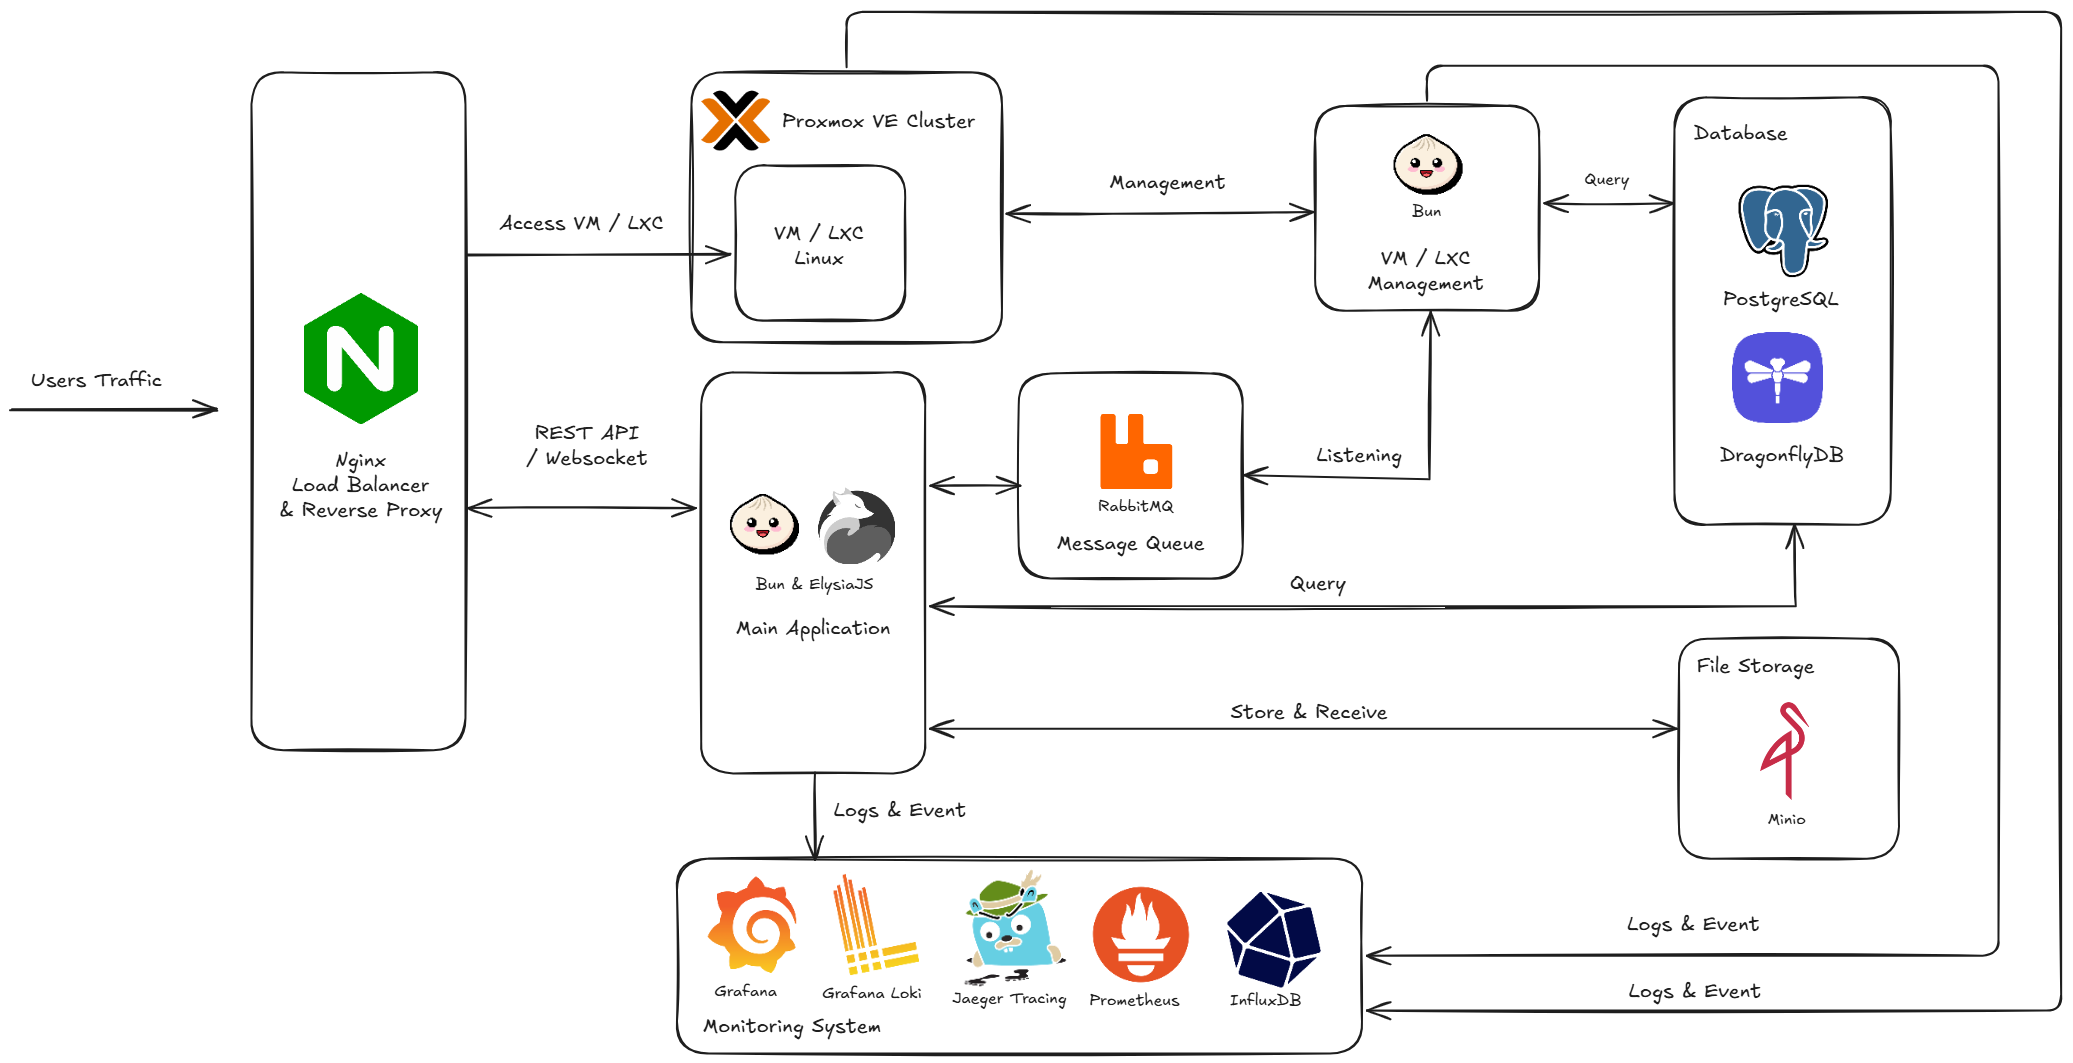
\includegraphics[width=0.9\textwidth]{./Image/web/system_architecture.png}
\caption{\fontSixTeen{สถาปัตยกรรมระบบ Cloud-Based Platform}}
\label{figD:SystemArchitecture}
\end{figure}

\section{บริการหลักและบทบาทในระบบ}
\hspace*{1.3em}
บริการหลักที่ใช้งานอยู่จริงใน code base ปัจจุบันมีดังนี้

\begin{mycustomenum2}
    \item \textbf{Midori} ทำหน้าที่เป็น frontend web application สำหรับนักศึกษา อาจารย์ และผู้ดูแลระบบ
    \item \textbf{Momoi} ทำหน้าที่เป็น API หลักของระบบ รับผิดชอบ business logic, OpenAPI, storage integration และ authentication endpoints
    \item \textbf{Yuzu} ทำหน้าที่เป็น background worker สำหรับจัดการ VM lifecycle บน Proxmox VE ผ่าน BullMQ
    \item \textbf{Satsuki} ทำหน้าที่เป็น automation service บนเครื่อง Nginx ภายนอก สำหรับสร้างไฟล์ reverse proxy configuration และ \textbf{authorized\_keys}
    \item \textbf{Yuuka} ทำหน้าที่เก็บ manifests, Docker Compose, observability configuration และเอกสารที่เกี่ยวข้องกับ deployment
\end{mycustomenum2}

\section{เทคโนโลยีที่ใช้ในการพัฒนา}
\hspace*{1.3em}
เทคโนโลยีที่ใช้งานจริงใน code base ปัจจุบันสามารถสรุปได้ดังนี้

\vspace{0.5em}
\textbf{Frontend Technologies}
\vspace{0.5em}

\begin{mycustomenum2}
    \item \textbf{Next.js 16} สำหรับพัฒนา Web Application แบบ React-based
    \item \textbf{React 19} สำหรับโครงสร้างส่วนติดต่อผู้ใช้
    \item \textbf{Tailwind CSS 4} สำหรับการจัดการรูปแบบหน้าจอ
    \item \textbf{TanStack React Query} สำหรับ data fetching และ state synchronization ฝั่ง client
    \item \textbf{better-auth client} สำหรับการเรียกใช้งาน authentication endpoints จากฝั่ง frontend
\end{mycustomenum2}

\vspace{0.5em}
\textbf{Backend และ Worker Technologies}
\vspace{0.5em}

\begin{mycustomenum2}
    \item \textbf{Bun} เป็น runtime หลักของ Momoi และ Yuzu
    \item \textbf{Elysia.js} เป็น web framework ของ Momoi
    \item \textbf{Prisma ORM} ใช้เข้าถึง PostgreSQL แบบ type-safe
    \item \textbf{PostgreSQL} เป็นฐานข้อมูลเชิงธุรกรรมหลักของระบบ
    \item \textbf{Redis} เป็น cache และ queue broker
    \item \textbf{BullMQ} เป็นระบบคิวงานระหว่าง Momoi และ Yuzu
    \item \textbf{better-auth} ใช้สำหรับ session และ OAuth flow ของระบบ
    \item \textbf{Zod} ใช้สำหรับ validation ของ environment variables และข้อมูลบางส่วนในระบบ
\end{mycustomenum2}

\vspace{0.5em}
\textbf{Virtualization และ Infrastructure}
\vspace{0.5em}

\begin{mycustomenum2}
    \item \textbf{Proxmox VE} เป็นแพลตฟอร์มหลักสำหรับจัดการ VM cluster
    \item \textbf{Kubernetes manifests} ในรีโพซิทอรี Yuuka ใช้สำหรับการติดตั้งบริการหลักในบางสภาพแวดล้อม
    \item \textbf{Docker Compose} ใช้สำหรับการเริ่มบริการประกอบในสภาพแวดล้อมพัฒนา
    \item \textbf{RustFS} ใช้เป็น S3-compatible object storage
    \item \textbf{Nginx} ทำหน้าที่เป็น reverse proxy หน้าด่านบนเครื่องภายนอก และรับการอัปเดต configuration จาก Satsuki
\end{mycustomenum2}

\section{ระบบคิวงานและการประมวลผลแบบ Asynchronous}
\hspace*{1.3em}
งานที่ใช้เวลานาน เช่น การสร้าง ลบ หรือเปลี่ยนสถานะ VM จะไม่ถูกประมวลผลภายใน request-response cycle ของ Momoi โดยตรง แต่จะถูกส่งเข้า Redis-backed BullMQ ก่อน จากนั้น Yuzu จะดึงงานไปประมวลผลแบบ asynchronous

\begin{mycustomenum2}
    \item \textbf{Provision Queue} สำหรับงานสร้าง VM ใหม่
    \item \textbf{Deprovision Queue} สำหรับงานลบหรือคืนทรัพยากรของ VM
    \item \textbf{Toggle Status Queue} สำหรับงาน Start, Stop และ Restart
\end{mycustomenum2}

\hspace*{1.3em}
ใน implementation ปัจจุบัน Yuzu รองรับการตั้งค่า concurrency แยกตามแต่ละคิวผ่าน environment variables และใช้ Redis-based distributed locks เพื่อกันงานที่ชน \textbf{instanceId} หรือ \textbf{VMID} เดียวกันไม่ให้ทำงานพร้อมกันโดยไม่จำเป็น

\section{Monitoring และ Observability}
\hspace*{1.3em}
ระบบมีการติดตามและตรวจสอบการทำงานอย่างครอบคลุมผ่านชุดเครื่องมือดังนี้

\begin{mycustomenum2}
    \item \textbf{Prometheus} สำหรับเก็บ metrics
    \item \textbf{Grafana} สำหรับสร้าง dashboards
    \item \textbf{Loki} สำหรับรวบรวม logs
    \item \textbf{Jaeger} สำหรับ distributed tracing
    \item \textbf{OpenTelemetry} เป็นมาตรฐานกลางสำหรับ telemetry data ของหลายบริการ
\end{mycustomenum2}

\section{ข้อดีของสถาปัตยกรรมที่เลือกใช้}
\hspace*{1.3em}
แนวทางสถาปัตยกรรมและเทคโนโลยีดังกล่าวมีข้อดีสำคัญดังนี้

\begin{mycustomenum2}
    \item แต่ละบริการสามารถพัฒนาและ deploy แยกกันได้ตามขอบเขตงาน
    \item Redis และ BullMQ ช่วยให้ระบบจัดการงานระยะยาวแบบ asynchronous ได้เหมาะสม
    \item การแยก Yuzu ออกจาก Momoi ช่วยลดภาระของ API หลักและเพิ่มความยืดหยุ่นในการ scaling
    \item Satsuki ช่วยทำให้ reverse proxy และ SSH access automation เชื่อมต่อกับข้อมูลในฐานข้อมูลได้โดยตรง
    \item OpenTelemetry, Prometheus และ Grafana ช่วยให้ติดตามปัญหาและวิเคราะห์ประสิทธิภาพของระบบได้ดีขึ้น
\end{mycustomenum2}

    % %*************************************
% ภาคผนวก จ.
%*************************************
\appendixChapterTitle{ค}{การ Deploy และการตั้งค่าสำหรับ Production}
\section{การ Deploy และการตั้งค่าสำหรับ Production}
\hspace*{1.3em}
การนำระบบ Cloud-Based Platform ไปใช้งานจริง (Production) ต้องมีการตั้งค่าและการเตรียมการที่แตกต่างจากการใช้งานในโหมด Development โดยมีรายละเอียดดังนี้

\vspace{0.5em}
\textbf{การเตรียมสภาพแวดล้อม Production}
\vspace{0.5em}

\begin{mycustomenum2}
    \item \textbf{ข้อกำหนดของ Server:}
    \begin{mycustomenum2}
        \item CPU: อย่างน้อย 8 cores (แนะนำ 16 cores หรือมากกว่า)
        \item RAM: อย่างน้อย 32 GB (แนะนำ 64 GB หรือมากกว่า)
        \item Storage: SSD อย่างน้อย 500 GB สำหรับ OS และ Applications
        \item Storage: HDD/SSD เพิ่มเติมสำหรับ VM Storage
        \item Network: การเชื่อมต่อเครือข่ายความเร็วสูงและเสถียร
    \end{mycustomenum2}

    \item \textbf{การติดตั้ง Proxmox VE:}
    \begin{mycustomenum2}
        \item ดาวน์โหลด Proxmox VE ISO จาก \url{https://www.proxmox.com/}
        \item ติดตั้งบน Server Hardware หรือ Virtual Machine
        \item ตั้งค่า Network และ Storage Pool
        \item สร้าง VM Templates สำหรับการใช้งาน
    \end{mycustomenum2}

    \item \textbf{การติดตั้งซอฟต์แวร์พื้นฐาน:}

\begin{figure}[htbp]
\centering
\adjustbox{frame, width=0.9\textwidth}{
    \begin{minipage}{0.85\textwidth}
        \texttt{\footnotesize
        \# Update system\\
        sudo apt update \&\& sudo apt upgrade -y\\
        \\
        \# Install Docker\\
        curl -fsSL https://get.docker.com -o get-docker.sh\\
        sudo sh get-docker.sh\\
        \\
        \# Install Docker Compose\\
        sudo apt install docker-compose-plugin\\
        \\
        \# Install Bun\\
        curl -fsSL https://bun.sh/install | bash
        }
    \end{minipage}
}
\caption{\fontSixTeen{การติดตั้งซอฟต์แวร์พื้นฐานสำหรับ Production}}
\label{figE:SoftwareInstall}
\end{figure}
\end{mycustomenum2}

\section{การตั้งค่า Environment Variables สำหรับ Production}
\hspace*{1.3em}
การตั้งค่า Environment Variables ที่เหมาะสมสำหรับการใช้งานจริง

\vspace{0.5em}
\textbf{ไฟล์ .env สำหรับ Production}
\vspace{0.5em}

\begin{figure}[htbp]
\centering
\adjustbox{frame, width=0.9\textwidth}{
    \begin{minipage}{0.85\textwidth}
        \texttt{\scriptsize
        \# Database Configuration\\
        DB\_HOST=localhost\\
        DB\_PORT=5432\\
        DB\_USER=cloudplatform\\
        DB\_PASSWORD=\{strong\_password\_here\}\\
        DB\_NAME=cloudplatform\_prod\\
        \\
        \# RabbitMQ Configuration\\
        RABBITMQ\_HOST=localhost\\
        RABBITMQ\_PORT=5672\\
        RABBITMQ\_USER=cloudplatform\\
        RABBITMQ\_PASSWORD=\{strong\_password\_here\}\\
        \\
        \# Proxmox Configuration\\
        PROXMOX\_HOST=\{proxmox\_server\_ip\}\\
        PROXMOX\_USERNAME=\{api\_username\}\\
        PROXMOX\_PASSWORD=\{api\_password\}\\
        PROXMOX\_NODE=\{proxmox\_node\_name\}\\
        \\
        \# Application Ports\\
        MIDORI\_PORT=3000\\
        MOMOI\_PORT=3001\\
        \\
        \# Security\\
        JWT\_SECRET=\{very\_strong\_jwt\_secret\}\\
        ENCRYPTION\_KEY=\{32\_char\_encryption\_key\}\\
        \\
        \# Monitoring\\
        JAEGER\_ENDPOINT=http://localhost:14268/api/traces\\
        PROMETHEUS\_PORT=9090\\
        LOKI\_ENDPOINT=http://localhost:3100
        }
    \end{minipage}
}
\caption{\fontSixTeen{ตัวอย่างการตั้งค่า Environment Variables สำหรับ Production}}
\label{figE:EnvProduction}
\end{figure}

\section{การ Deploy ด้วย Docker Compose}
\hspace*{1.3em}
การใช้ Docker Compose สำหรับการ Deploy ระบบแบบ Production

\vspace{0.5em}
\textbf{การสร้าง Production Docker Compose}
\vspace{0.5em}

\begin{mycustomenum2}
    \item สร้างไฟล์ \texttt{docker-compose.prod.yml}

\begin{figure}[htbp]
\centering
\adjustbox{frame, width=0.9\textwidth}{
    \begin{minipage}{0.85\textwidth}
        \texttt{\scriptsize
        version: '3.8'\\
        \\
        services:\\
        \hspace*{1em}midori:\\
        \hspace*{2em}build:\\
        \hspace*{3em}context: .\\
        \hspace*{3em}dockerfile: docker/midori.dockerfile\\
        \hspace*{2em}ports:\\
        \hspace*{3em}- "\$\{MIDORI\_PORT:-3000\}:3000"\\
        \hspace*{2em}environment:\\
        \hspace*{3em}- NODE\_ENV=production\\
        \hspace*{3em}- MOMOI\_API\_URL=http://momoi:3001\\
        \hspace*{2em}depends\_on:\\
        \hspace*{3em}- momoi\\
        \hspace*{2em}restart: unless-stopped\\
        \\
        \hspace*{1em}momoi:\\
        \hspace*{2em}build:\\
        \hspace*{3em}context: .\\
        \hspace*{3em}dockerfile: docker/momoi.dockerfile\\
        \hspace*{2em}ports:\\
        \hspace*{3em}- "\$\{MOMOI\_PORT:-3001\}:3001"\\
        \hspace*{2em}environment:\\
        \hspace*{3em}- NODE\_ENV=production\\
        \hspace*{2em}depends\_on:\\
        \hspace*{3em}- db\\
        \hspace*{3em}- queue\\
        \hspace*{2em}restart: unless-stopped
        }
    \end{minipage}
}
\caption{\fontSixTeen{ตัวอย่าง Docker Compose สำหรับ Production}}
\label{figE:DockerComposeProduction}
\end{figure}

    \item รันคำสั่งสำหรับ Deploy

\begin{figure}[htbp]
\centering
\adjustbox{frame, width=0.9\textwidth}{
    \begin{minipage}{0.85\textwidth}
        \texttt{\footnotesize
        \# Build และ Start Services\\
        docker-compose -f docker-compose.prod.yml up -d --build\\
        \\
        \# ตรวจสอบสถานะ Services\\
        docker-compose -f docker-compose.prod.yml ps\\
        \\
        \# ดู Logs\\
        docker-compose -f docker-compose.prod.yml logs -f
        }
    \end{minipage}
}
\caption{\fontSixTeen{คำสั่งสำหรับ Deploy ด้วย Docker Compose}}
\label{figE:DockerDeployCommands}
\end{figure}
\end{mycustomenum2}

\section{การตั้งค่า Reverse Proxy และ SSL}
\hspace*{1.3em}
การตั้งค่า Nginx เป็น Reverse Proxy และการติดตั้ง SSL Certificate

\vspace{0.5em}
\textbf{การติดตั้งและตั้งค่า Nginx}
\vspace{0.5em}

\begin{mycustomenum2}
    \item ติดตั้ง Nginx

\begin{figure}[htbp]
\centering
\adjustbox{frame, width=0.9\textwidth}{
    \begin{minipage}{0.85\textwidth}
        \texttt{\footnotesize
        sudo apt install nginx\\
        sudo systemctl enable nginx\\
        sudo systemctl start nginx
        }
    \end{minipage}
}
\caption{\fontSixTeen{การติดตั้ง Nginx}}
\label{figE:NginxInstall}
\end{figure}

    \item สร้างไฟล์ Configuration สำหรับ Site

\begin{figure}[htbp]
\centering
\adjustbox{frame, width=0.9\textwidth}{
    \begin{minipage}{0.85\textwidth}
        \texttt{\scriptsize
        server \{\\
        \hspace*{1em}listen 80;\\
        \hspace*{1em}server\_name your-domain.com;\\
        \\
        \hspace*{1em}location / \{\\
        \hspace*{2em}proxy\_pass http://localhost:3000;\\
        \hspace*{2em}proxy\_http\_version 1.1;\\
        \hspace*{2em}proxy\_set\_header Upgrade \$http\_upgrade;\\
        \hspace*{2em}proxy\_set\_header Connection 'upgrade';\\
        \hspace*{2em}proxy\_set\_header Host \$host;\\
        \hspace*{2em}proxy\_set\_header X-Real-IP \$remote\_addr;\\
        \hspace*{2em}proxy\_set\_header X-Forwarded-For \$proxy\_add\_x\_forwarded\_for;\\
        \hspace*{2em}proxy\_set\_header X-Forwarded-Proto \$scheme;\\
        \hspace*{2em}proxy\_cache\_bypass \$http\_upgrade;\\
        \hspace*{1em}\}\\
        \\
        \hspace*{1em}location /api \{\\
        \hspace*{2em}proxy\_pass http://localhost:3001;\\
        \hspace*{2em}proxy\_set\_header Host \$host;\\
        \hspace*{2em}proxy\_set\_header X-Real-IP \$remote\_addr;\\
        \hspace*{2em}proxy\_set\_header X-Forwarded-For \$proxy\_add\_x\_forwarded\_for;\\
        \hspace*{2em}proxy\_set\_header X-Forwarded-Proto \$scheme;\\
        \hspace*{1em}\}\\
        \}
        }
    \end{minipage}
}
\caption{\fontSixTeen{การตั้งค่า Nginx Reverse Proxy}}
\label{figE:NginxConfig}
\end{figure}

    \item ติดตั้ง SSL Certificate ด้วย Let's Encrypt

\begin{figure}[htbp]
\centering
\adjustbox{frame, width=0.9\textwidth}{
    \begin{minipage}{0.85\textwidth}
        \texttt{\footnotesize
        \# ติดตั้ง Certbot\\
        sudo apt install certbot python3-certbot-nginx\\
        \\
        \# ขอ SSL Certificate\\
        sudo certbot --nginx -d your-domain.com\\
        \\
        \# ตั้งค่า Auto-renewal\\
        sudo crontab -e\\
        \# เพิ่มบรรทัด: 0 12 * * * /usr/bin/certbot renew --quiet
        }
    \end{minipage}
}
\caption{\fontSixTeen{การติดตั้ง SSL Certificate}}
\label{figE:SSLInstall}
\end{figure}
\end{mycustomenum2}

\section{การตั้งค่า Database สำหรับ Production}
\hspace*{1.3em}
การเตรียม PostgreSQL Database สำหรับการใช้งานจริง

\vspace{0.5em}
\textbf{การตั้งค่า PostgreSQL}
\vspace{0.5em}

\begin{mycustomenum2}
    \item การตั้งค่า Database User และ Permissions

\begin{figure}[htbp]
\centering
\adjustbox{frame, width=0.9\textwidth}{
    \begin{minipage}{0.85\textwidth}
        \texttt{\footnotesize
        \# เข้าสู่ PostgreSQL\\
        sudo -u postgres psql\\
        \\
        \# สร้าง Database และ User\\
        CREATE DATABASE cloudplatform\_prod;\\
        CREATE USER cloudplatform WITH ENCRYPTED PASSWORD 'strong\_password';\\
        GRANT ALL PRIVILEGES ON DATABASE cloudplatform\_prod TO cloudplatform;\\
        \\
        \# ออกจาก PostgreSQL\\
        \\q
        }
    \end{minipage}
}
\caption{\fontSixTeen{การตั้งค่า PostgreSQL Database}}
\label{figE:PostgreSQLSetup}
\end{figure}

    \item การรัน Database Migration

\begin{figure}[htbp]
\centering
\adjustbox{frame, width=0.9\textwidth}{
    \begin{minipage}{0.85\textwidth}
        \texttt{\footnotesize
        \# เข้าไปใน Momoi directory\\
        cd apps/momoi\\
        \\
        \# รัน Prisma Migration\\
        bunx prisma migrate deploy\\
        \\
        \# Generate Prisma Client\\
        bunx prisma generate
        }
    \end{minipage}
}
\caption{\fontSixTeen{การรัน Database Migration}}
\label{figE:DatabaseMigration}
\end{figure}

    \item การตั้งค่า Database Backup

\begin{figure}[htbp]
\centering
\adjustbox{frame, width=0.9\textwidth}{
    \begin{minipage}{0.85\textwidth}
        \texttt{\footnotesize
        \#!/bin/bash\\
        \# สร้างไฟล์ backup-db.sh\\
        \\
        DB\_NAME="cloudplatform\_prod"\\
        DB\_USER="cloudplatform"\\
        BACKUP\_DIR="/backups/postgresql"\\
        DATE=\$(date +\%Y\%m\%d\_\%H\%M\%S)\\
        \\
        \# สร้าง directory หากไม่มี\\
        mkdir -p \$BACKUP\_DIR\\
        \\
        \# สำรอง Database\\
        pg\_dump -h localhost -U \$DB\_USER -d \$DB\_NAME > \\
        \hspace*{1em}\$BACKUP\_DIR/backup\_\$DATE.sql\\
        \\
        \# ลบไฟล์ backup เก่าที่เก็บเกิน 7 วัน\\
        find \$BACKUP\_DIR -name "backup\_*.sql" -mtime +7 -delete
        }
    \end{minipage}
}
\caption{\fontSixTeen{สคริปต์สำหรับ Database Backup}}
\label{figE:DatabaseBackup}
\end{figure}
\end{mycustomenum2}

\section{การตรวจสอบและบำรุงรักษาระบบ}
\hspace*{1.3em}
การตรวจสอบและบำรุงรักษาระบบเพื่อให้ทำงานได้อย่างเสถียร

\vspace{0.5em}
\textbf{การตรวจสอบสถานะระบบ}
\vspace{0.5em}

\begin{mycustomenum2}
    \item สร้างสคริปต์ตรวจสอบสถานะ Services

\begin{figure}[htbp]
\centering
\adjustbox{frame, width=0.9\textwidth}{
    \begin{minipage}{0.85\textwidth}
        \texttt{\footnotesize
        \#!/bin/bash\\
        \# สร้างไฟล์ health-check.sh\\
        \\
        echo "=== System Health Check ==="\\
        \\
        \# ตรวจสอบ Docker Services\\
        echo "Docker Services Status:"\\
        docker-compose -f docker-compose.prod.yml ps\\
        \\
        \# ตรวจสอบ Nginx\\
        echo "Nginx Status:"\\
        systemctl status nginx --no-pager\\
        \\
        \# ตรวจสอบ Disk Space\\
        echo "Disk Usage:"\\
        df -h\\
        \\
        \# ตรวจสอบ Memory\\
        echo "Memory Usage:"\\
        free -h\\
        \\
        \# ตรวจสอบการเชื่อมต่อ Database\\
        echo "Database Connection:"\\
        pg\_isready -h localhost -p 5432
        }
    \end{minipage}
}
\caption{\fontSixTeen{สคริปต์ตรวจสอบสถานะระบบ}}
\label{figE:HealthCheck}
\end{figure}

    \item ตั้งค่า Cron Job สำหรับการตรวจสอบอัตโนมัติ

\begin{figure}[htbp]
\centering
\adjustbox{frame, width=0.9\textwidth}{
    \begin{minipage}{0.85\textwidth}
        \texttt{\footnotesize
        \# แก้ไข Crontab\\
        crontab -e\\
        \\
        \# เพิ่มงานตรวจสอบทุก 5 นาที\\
        */5 * * * * /path/to/health-check.sh >> /var/log/health-check.log\\
        \\
        \# สำรอง Database ทุกวันเวลา 2:00 น.\\
        0 2 * * * /path/to/backup-db.sh\\
        \\
        \# ทำความสะอาด Docker images เก่าทุกอาทิตย์\\
        0 3 * * 0 docker system prune -f
        }
    \end{minipage}
}
\caption{\fontSixTeen{การตั้งค่า Cron Jobs}}
\label{figE:CronJobs}
\end{figure}
\end{mycustomenum2}

\vspace{0.5em}
\textbf{การอัปเดตระบบ}
\vspace{0.5em}

\begin{mycustomenum2}
    \item การอัปเดตแอปพลิเคชัน

\begin{figure}[htbp]
\centering
\adjustbox{frame, width=0.9\textwidth}{
    \begin{minipage}{0.85\textwidth}
        \texttt{\footnotesize
        \#!/bin/bash\\
        \# สร้างไฟล์ update-app.sh\\
        \\
        echo "Starting application update..."\\
        \\
        \# Pull latest code\\
        git pull origin main\\
        \\
        \# Install dependencies\\
        bun install\\
        \\
        \# Build และ restart services\\
        docker-compose -f docker-compose.prod.yml down\\
        docker-compose -f docker-compose.prod.yml up -d --build\\
        \\
        \# ตรวจสอบสถานะหลัง update\\
        sleep 30\\
        docker-compose -f docker-compose.prod.yml ps\\
        \\
        echo "Update completed!"
        }
    \end{minipage}
}
\caption{\fontSixTeen{สคริปต์สำหรับอัปเดตแอปพลิเคชัน}}
\label{figE:UpdateApp}
\end{figure}
\end{mycustomenum2}

\section{การแก้ไขปัญหาใน Production}
\hspace*{1.3em}
วิธีการแก้ไขปัญหาที่อาจเกิดขึ้นในการใช้งานจริง

\vspace{0.5em}
\textbf{ปัญหาที่พบบ่อยและวิธีแก้ไข}
\vspace{0.5em}

\begin{mycustomenum2}
    \item \textbf{Service ไม่ตอบสนอง}
    \begin{mycustomenum2}
        \item ตรวจสอบ Logs: \texttt{docker-compose logs [service\_name]}
        \item รีสตาร์ท Service: \texttt{docker-compose restart [service\_name]}
        \item ตรวจสอบ Resource Usage: \texttt{docker stats}
    \end{mycustomenum2}

    \item \textbf{Database Connection Error}
    \begin{mycustomenum2}
        \item ตรวจสอบ PostgreSQL Service: \texttt{systemctl status postgresql}
        \item ตรวจสอบ Connection Pool: ดู Logs ของ Momoi Service
        \item รีสตาร์ท Database: \texttt{sudo systemctl restart postgresql}
    \end{mycustomenum2}

    \item \textbf{Out of Disk Space}
    \begin{mycustomenum2}
        \item ทำความสะอาด Docker: \texttt{docker system prune -a}
        \item ลบ Log files เก่า: \texttt{find /var/log -name "*.log" -mtime +30 -delete}
        \item ตรวจสอบ VM Storage ใน Proxmox
    \end{mycustomenum2}

    \item \textbf{SSL Certificate หมดอายุ}
    \begin{mycustomenum2}
        \item ต่ออายุ Certificate: \texttt{sudo certbot renew}
        \item รีโหลด Nginx: \texttt{sudo nginx -s reload}
        \item ตรวจสอบวันหมดอายุ: \texttt{sudo certbot certificates}
    \end{mycustomenum2}
\end{mycustomenum2}

\end{document}
